%%%%%%%%%%%%%%%%%%%%%%%%%%%%%%%%%%%%%%%%%%%%%%%%%%%%%%%%%%%%%%%%%%%%%%
% Template-TA-Fisika-ITS.v.1.0 2022.01
%%%%%%%%%%%%%%%%%%%%%%%%%%%%%%%%%%%%%%%%%%%%%%%%%%%%%%%%%%%%%%%%%%%%%%
% oleh: 1. Sasfan Arman Wella, BRIN (sasfan.a.wella@gmail.com)
%       2. Nadya Amalia, BRIN (amalianadd@gmail.com)
%       3. Fitrotul Millah, ITS (fitrotulmillah2000@gmail.com)
%       4. Nathasya Veronica, ITS (nathasyaveronica363@gmail.com) 
%
%  NB: Template ini bukanlah template resmi dari ITS, namun disusun
%      berdasarkan pedoman penulisan laporan TA Fisika ITS
%
% [ Bila ada fitur yang ditambahkan dalam template ini, silahkan
%   tambahkan nama Anda setelah nama pembuat template sebelumnya ]
%
%  Penjelasan singkat dari template ini 
%  dapat dilihat pada file README
% 
%%%%%%%%%%%%%%%%%%%%%%%%%%%%%%%%%%%%%%%%%%%%%%%%%%%%%%%%%%%%%%%%%%%%%%

%=====================================================================
% FORMAT DAN PENGATURAN UMUM:
%=====================================================================
\documentclass[a4paper, 12pt, final, openright, oneside]{report}
%%%%%%%%%%%%%%%%%%%%%%%%%%%%%%%%%%%%%%%%%%%%%%%%%%%%%%%%%%%%%%%%%%%%%%
% FORMAT DAN PENGATURAN UMUM:
%=====================================================================
\usepackage{multirow}
\usepackage[table]{xcolor}
\usepackage{tabularx,tikz}
\usepackage{caption}
\usepackage{float}
\usepackage{listings}
\usepackage{subcaption}
\usepackage{graphicx}
\usepackage{enumitem}
\usepackage{amsmath,amssymb,amsfonts,charter,color}\usepackage[hidelinks]{hyperref}
\usepackage[utf8]{inputenc}
\usepackage{lipsum} % hanya untuk membuat teks dummy
\usepackage{wrapfig}
\usepackage{emptypage}
\usepackage{setspace}
\usepackage{rotating}
\usepackage{colortbl}       % Tambahan untuk mendukung \rowcolor dan \cellcolor
\usepackage{pgfgantt} 
\usepackage[bahasa]{babel}
\usepackage{fontenc}
\usepackage{graphicx}
\usepackage{geometry}
\usepackage{setspace}
\onehalfspacing
\usepackage{times}
\usepackage{caption}
\captionsetup{justification=centering, singlelinecheck=false, labelfont=bf, labelsep=period}
\usepackage{booktabs} % For better table rules
\usepackage{longtable} % For tables that might span pages
\usepackage{array} % For table column formatting

%======================================================================
%   Mengatur margin 
%======================================================================
\usepackage[top=3cm,left=3cm,right=2cm,bottom=2.5cm]{geometry}
    \linespread{1.3} % Gunakan 1.3 untuk spasi satu setengah, 
                     % Gunakan 1.6 untukspasi dua
    
%======================================================================
%   Mengatur bahasa yang digunakan
%======================================================================

\usepackage[bahasa]{babel}
    \selectlanguage{bahasa}

%======================================================================
%   Mengatur format BAB, SUBBAB, Floating Gambar dan Tabel
%======================================================================

\usepackage[explicit]{titlesec}
    \titleformat{\chapter}[display]
        {\normalfont\bfseries\centering}
        {\large\MakeUppercase{\chaptername}~\thechapter}
        {0.5em}{\large \MakeUppercase{#1}}
    \titleformat{\section}
        {\normalfont\normalsize\bfseries}{\thesection}
        {0.5em}{#1}
    \titleformat{\subsection}
        {\normalfont\normalsize\bfseries}{\thesubsection}
        {0.5em}{#1}
    
\usepackage{tocloft,etoolbox}
\apptocmd{\appendix}
    {\addtocontents{toc}{  
    \protect\addtolength\protect\cftchapnumwidth{-\mylength}
    \protect\renewcommand{\protect\cftchappresnum}{LAMPIRAN~}
    \protect\settowidth\mylength{
    \bfseries\protect\cftchappresnum\protect\cftchapaftersnum}
    \protect\addtolength\protect\cftchapnumwidth{\mylength}}}{}{}
\newlength\mylength

\renewcommand\cftchappresnum{BAB~}
\settowidth\mylength{\bfseries\cftchappresnum\cftchapaftersnum}
\addtolength\cftchapnumwidth{\mylength}
\renewcommand{\cftdotsep}{1}
\renewcommand{\cftchapleader}{\cftdotfill{\cftsecdotsep}}

\renewcommand\cftfigpresnum{Gambar~}
\settowidth\mylength{\cftfigpresnum\cftfigaftersnum}
\addtolength\cftfignumwidth{\mylength}

\renewcommand\cfttabpresnum{Tabel~}
\settowidth\mylength{\cfttabpresnum\cfttabaftersnum}
\addtolength\cfttabnumwidth{\mylength}

%======================================================================
%   Mengatur background pada cover
%======================================================================
\usepackage[pages=some]{background}
\backgroundsetup{
    scale=1,
    color=black,
    opacity=1.0,
    angle=0,
    contents={%
    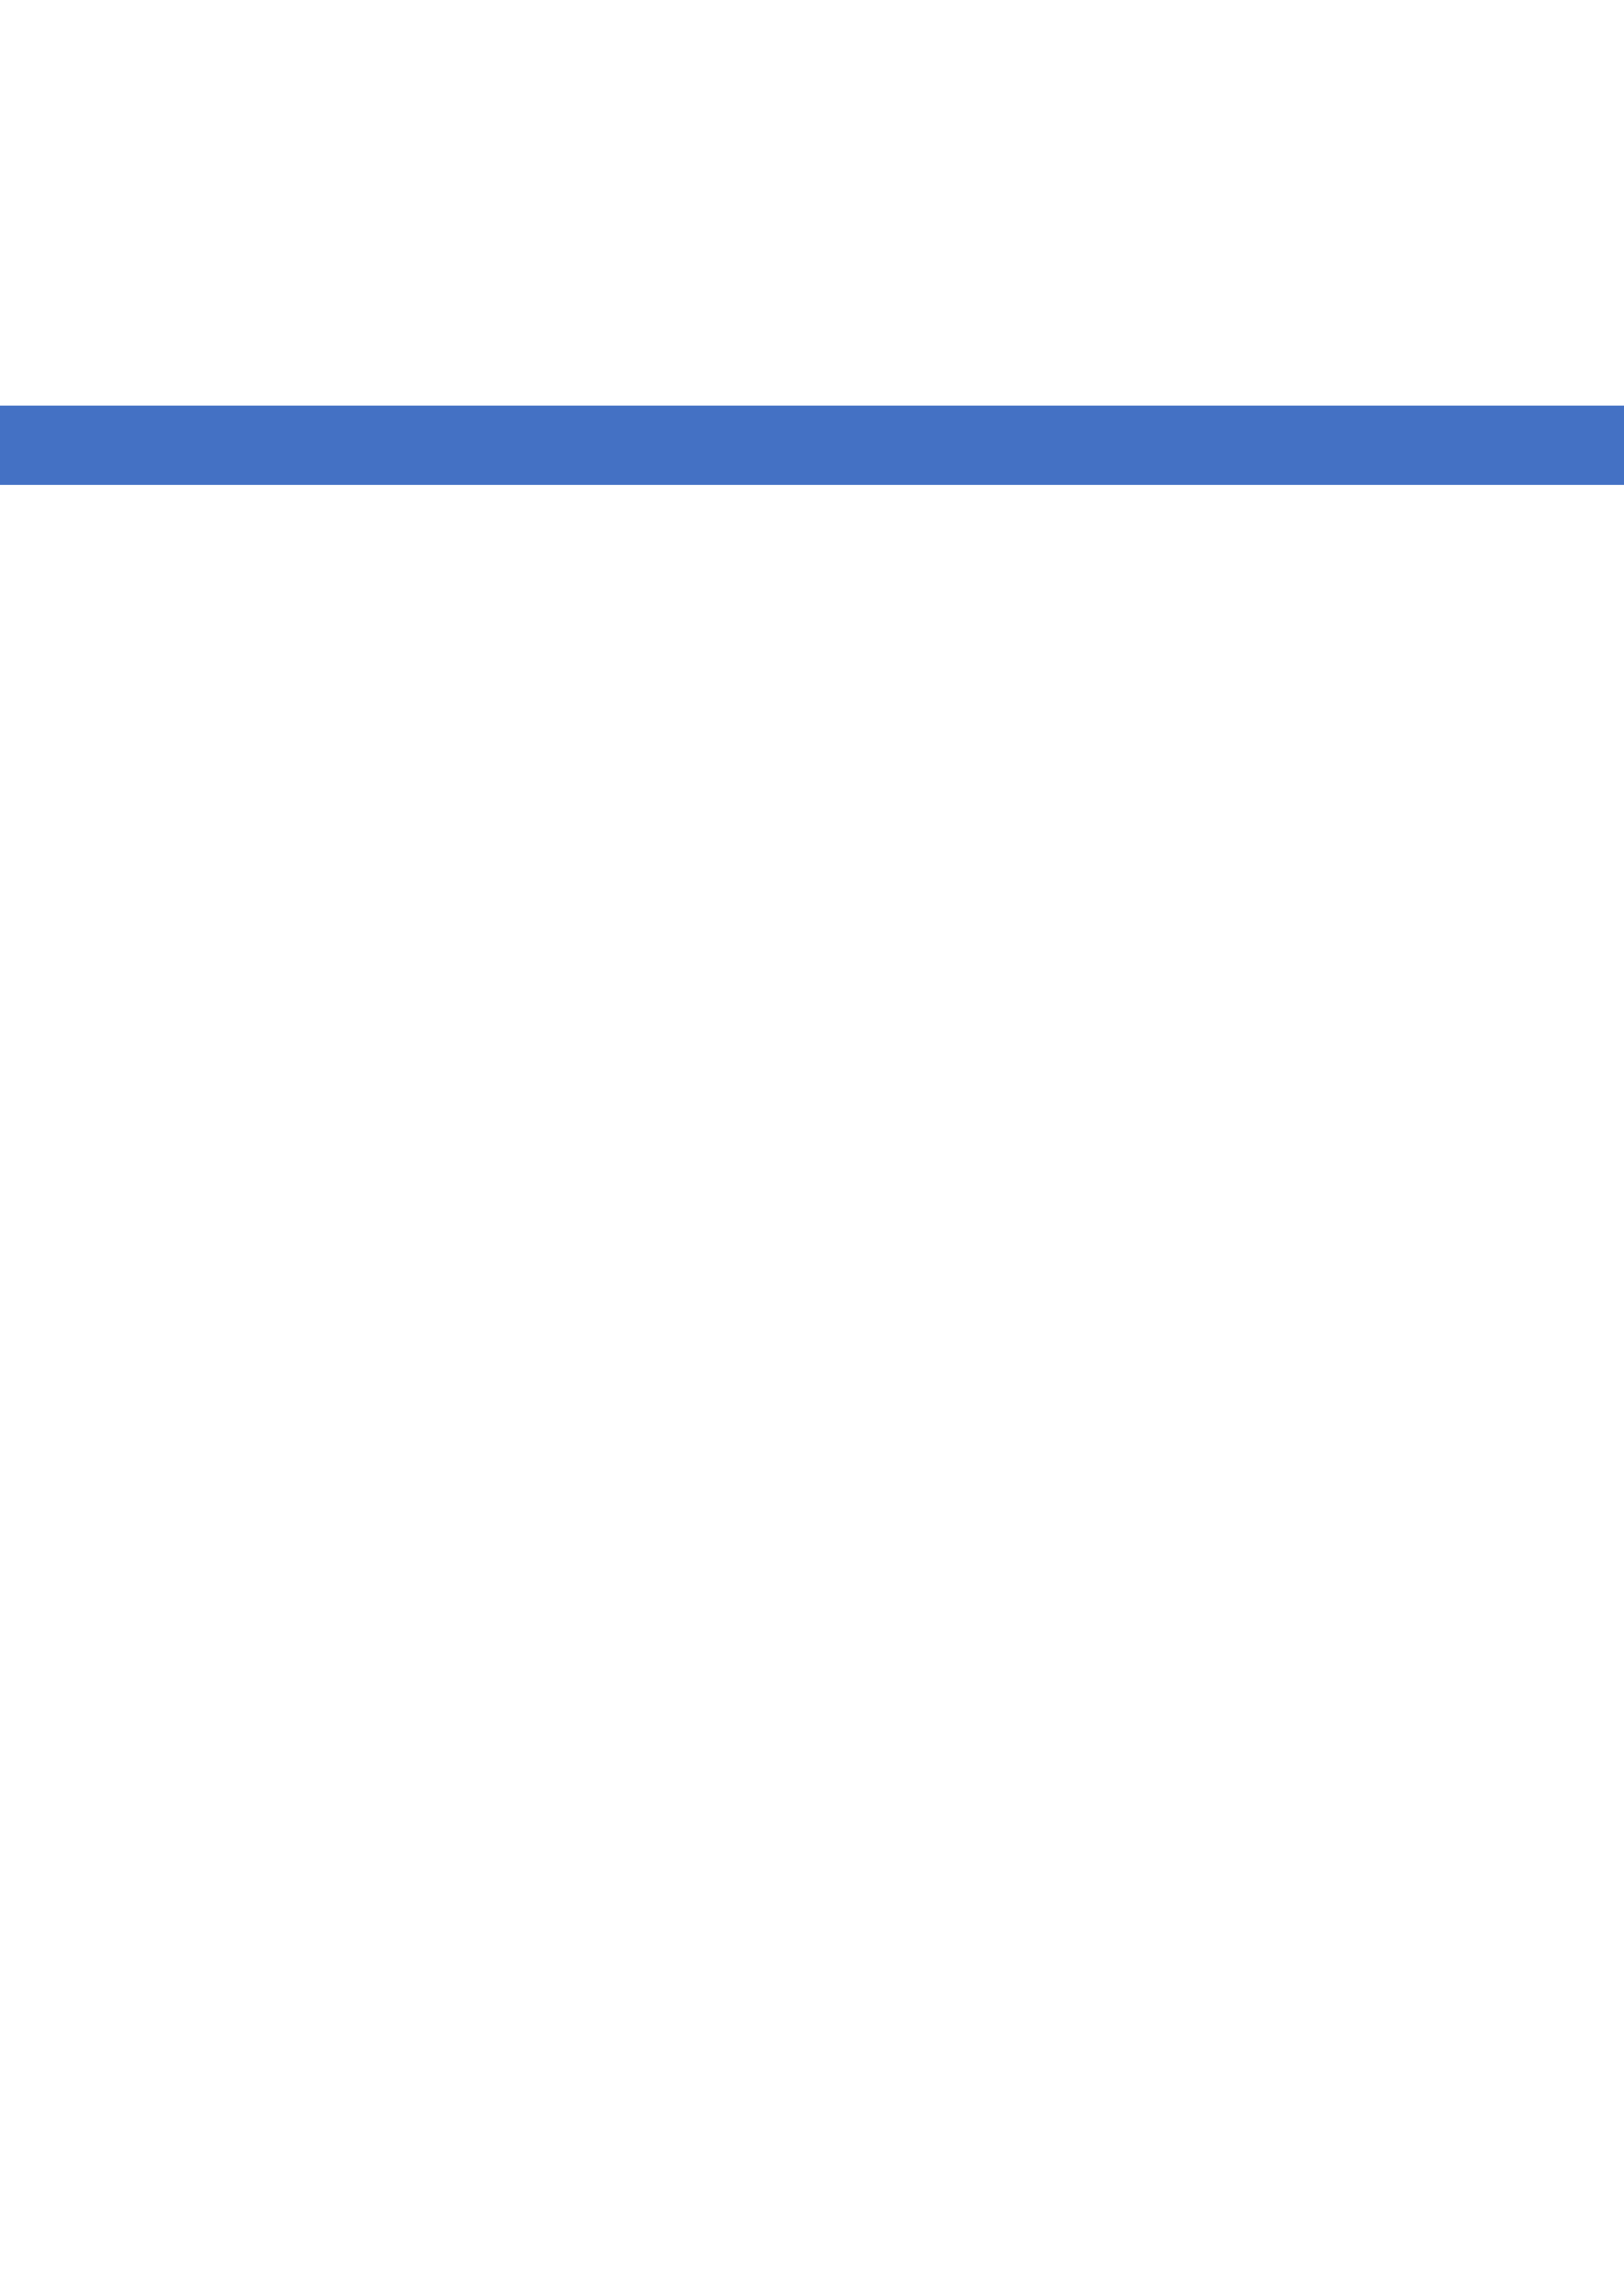
\includegraphics[width=\paperwidth,height=\paperheight]
    {./gambar/cover_prop_d-1.png}
    }%
}

%======================================================================
%   Mengatur jenis font yang digunakan
%======================================================================
\usepackage{fontspec}
\setmainfont{Times New Roman} 
\setsansfont{Trebuchet MS} 
\setmonofont{Inconsolata}

%======================================================================
%   Untuk mendefinisikan halaman kosong
%======================================================================
\newcommand\halamanKosong{
    \newpage
    \vspace*{\fill}
    \begin{center}
        \textit{Halaman ini sengaja dikosongkan}
    \end{center}
    \vspace{\fill}
    \clearpage
}

%======================================================================
%   Mengatur agar paragraf pertama mempunyai indentasi
%======================================================================
\usepackage{indentfirst}
\setlength{\parindent}{2em} 

%======================================================================
%   Mengatur tentang jarak antara judul section dan paragraf
%======================================================================
\usepackage{titlesec}

\titlespacing\section{0pt}{12pt plus 4pt minus 2pt}{0pt plus 2pt minus 2pt}
\titlespacing\subsection{0pt}{12pt plus 4pt minus 2pt}{0pt plus 2pt minus 2pt}
\titlespacing\subsubsection{0pt}{12pt plus 4pt minus 2pt}{0pt plus 2pt minus 2pt}

%======================================================================
%   Mengatur header dan footer
%======================================================================
\usepackage{fancyhdr}
    \fancyhead{}
    \fancyfoot{}
    \setlength{\headheight}{15pt}
    \setlength{\headsep}{12pt}
    \setlength{\footskip}{30pt}
    \renewcommand{\headrulewidth}{0pt}
    \renewcommand{\footrulewidth}{0pt}
    
    \fancypagestyle{romawi}{%
    \setlength{\headheight}{15pt}
    \setlength{\headsep}{12pt}
    \setlength{\footskip}{30pt}
    \fancyfoot[CE,CO]{\thepage}
    \renewcommand{\headrulewidth}{0pt}
    \renewcommand{\footrulewidth}{0pt}
    }
    
    \fancypagestyle{konten}{%
    \setlength{\headheight}{15pt}
    \setlength{\headsep}{12pt}
    \setlength{\footskip}{30pt}
    \fancyhead[LE,RO]{\thepage}
    \fancyfoot[CE,CO]{}
    \renewcommand{\headrulewidth}{0pt}
    \renewcommand{\footrulewidth}{0pt}
    }
    
%======================================================================
%   Mengatur tentang format referensi
%======================================================================

\usepackage[square]{natbib}

%======================================================================
%   Mengatur template untuk menulis code
%======================================================================

\usepackage{listings}
\usepackage[framemethod=default]{mdframed}

\newmdenv[innerlinewidth=0.5pt, 
roundcorner=4pt,
linecolor=red,
innerleftmargin=6pt,
innerrightmargin=6pt,
innertopmargin=6pt,
innerbottommargin=6pt,
backgroundcolor=red,
]{mybox}
\newcommand{\unitcell}{\textit{unit cell }}
\newcommand{\exchange}{\textit{exchange }}
\newcommand{\corr}{\textit{correlation }}
\newcommand{\eh}[1]{{\color{red} EH:{#1}}}
\newcommand{\schro}{Schr{\"o}dinger }
\newcommand{\be}{\begin{equation}}
\newcommand{\ee}{\end{equation}}
\newcommand{\bea}{\begin{eqnarray}}
\newcommand{\eea}{\end{eqnarray}}
\newcommand{\HH}{{\cal H}}
\newcommand{\RR}{{\cal R}}
\newcommand{\p}{\partial}
\newcommand{\s}{\sigma}
\newcommand{\la}{\langle}
\newcommand{\ra}{\rangle}
\newcommand{\lla}{\left\langle}
\newcommand{\rra}{\right\rangle}
\newcommand{\lb}{\left[}
\newcommand{\rb}{\right]}
\newcommand{\lp}{\left(}
\newcommand{\rp}{\right)}
\newcommand{\Tr}{{\rm \, Tr\,}}
\newcommand{\bra}[1]{\la #1|}
\newcommand{\ket}[1]{| #1\ra}
\newcommand{\sgn}{{\rm sgn}\,}
\renewcommand{\Im}{{\rm Im}\,}
\renewcommand{\Re}{{\rm Re}\,}
\renewcommand{\vec}[1]{{\bf #1}}
\newcommand{\eps}{\varepsilon}
\renewcommand{\tilde}{\widetilde}
\def\nn{\nonumber\\}

\definecolor{codegreen}{rgb}{0,0.6,0}
\definecolor{codegray}{rgb}{0.5,0.5,0.5}
\definecolor{codepurple}{rgb}{0.58,0,0.82}
\definecolor{backcolour}{rgb}{0.95,0.95,0.92}

\lstdefinestyle{mystyle}{
    backgroundcolor=\color{backcolour},   
    commentstyle=\color{codegreen},
    keywordstyle=\color{magenta},
    numberstyle=\tiny\color{codegray},
    stringstyle=\color{codepurple},
    basicstyle=\ttfamily\small,
    breakatwhitespace=false,         
    breaklines=true,                 
    captionpos=b,                    
    keepspaces=true,                 
    numbers=left,                    
    numbersep=5pt,                  
    showspaces=false,                
    showstringspaces=false,
    showtabs=false,                  
    tabsize=2 
}

\lstset{style=mystyle}

%======================================================================
%   Agar sisi bagian kanan menjadi lebih rapih
%======================================================================
\emergencystretch=\maxdimen
\hyphenpenalty=10000
\hbadness=10000

%======================================================================
%   Mengatur jenis font untuk equations
%======================================================================
\usepackage{newtxmath}

%======================================================================
%   Mengatur format daftar isi, gambar, dan tabel
%======================================================================

\renewcommand{\cfttoctitlefont}{\hfil\large\bfseries\MakeUppercase}
\renewcommand{\cftloftitlefont}{\hfil\large\bfseries\MakeUppercase}
\renewcommand{\cftlottitlefont}{\hfil\large\bfseries\MakeUppercase}
\renewcommand{\cftsecleader}{\cftdotfill{\cftdotsep}}
\setlength\cftparskip{-2pt}
\setlength\cftbeforesecskip{2pt}
\setlength\cftbeforechapskip{2pt}
\setlength\extrarowheight{5pt}

%======================================================================
%   Mengatur Diagram Alir
%======================================================================
\usepackage{tikz}
\usetikzlibrary{shapes.geometric, arrows}

\definecolor{adaee4ed-88c8-5b21-a9e7-31316ebef86f}{RGB}{255, 179, 178}
\definecolor{f3551e38-74df-57e2-b793-83d7fe876c85}{RGB}{0, 0, 0}
\definecolor{0b71a967-1f15-55a5-9bb9-70efa7b4fc58}{RGB}{51, 51, 51}
\definecolor{747aec21-333b-59ee-84e3-ddff893e5ccd}{RGB}{255, 216, 176}
\definecolor{5856d031-3da1-575c-834e-c77e9e438c62}{RGB}{162, 177, 195}

\tikzstyle{512bdd77-c3aa-5669-a956-85f7a90c6fb4} = [rectangle, rounded corners, minimum width=3cm, minimum height=1cm, text centered, font=\normalsize, color=0b71a967-1f15-55a5-9bb9-70efa7b4fc58, draw=f3551e38-74df-57e2-b793-83d7fe876c85, line width=1, fill=adaee4ed-88c8-5b21-a9e7-31316ebef86f]
\tikzstyle{69bbb168-da59-5865-902f-94e77902bf95} = [rectangle, minimum width=3cm, minimum height=1cm, text centered, font=\normalsize, color=0b71a967-1f15-55a5-9bb9-70efa7b4fc58, draw=f3551e38-74df-57e2-b793-83d7fe876c85, line width=1, fill=747aec21-333b-59ee-84e3-ddff893e5ccd]
\tikzstyle{40b3368b-3948-5ae0-af87-93343251acd0} = [rectangle, minimum width=4cm, minimum height=1cm, text centered, font=\normalsize, color=0b71a967-1f15-55a5-9bb9-70efa7b4fc58, draw=f3551e38-74df-57e2-b793-83d7fe876c85, line width=1, fill=747aec21-333b-59ee-84e3-ddff893e5ccd]
\tikzstyle{7be24b85-97d0-5b76-ba9e-d94005dca8f2} = [thick, draw=5856d031-3da1-575c-834e-c77e9e438c62, line width=2, ->, >=stealth]


\tikzstyle{startstop} = [ellipse, minimum width=3cm, minimum height=1cm, text centered, draw=black]
\tikzstyle{process} = [rectangle, minimum width=3cm, minimum height=1cm, text centered, draw=black]
\tikzstyle{arrow} = [thick,->,>=stealth]
%%%%%%%%%%%%%%%%%%%%%%%%%%%%%%%%%%%%%%%%%%%%%%%%%%%%%%%%%%%%%%%%%%%%%%

%%%%%%%%%%%%%%%%%%%%%%%%%%%%%%%%%%%%%%%%%%%%%%%%%%%%%%%%%%%%%%%%%%%%%%
% TULISKAN INFORMASI-INFORMASI YANG DIBUTUHKAN DALAM DOKUMEN TUGAS AKHIR
%=====================================================================
% Judul Tugas Akhir
\newcommand{\kodeTA}{
    TUGAS AKHIR% Tuliskan kode mata kuliah dalam bahasa Indonesia
}
\newcommand{\kodeTAInggris}{
    FINAL REPORT% Tuliskan kode mata kuliah dalam bahasa Inggris
} 
%=====================================================================
% Judul Tugas Akhir
\newcommand{\judulTA}{%
Analisis Sifat Elektronik dan Magnetik dari Struktur Boron Nitride heksagonal Akibat Perlakuan Termal Melalui Studi Teori Densitas Kerapatan dan Dinamika Molekul % Tuliskan judul dalam bahasa Indonesia
}
\newcommand{\judulTAInggris}{
    ANALYSIS OF ELECTRONIC AND MAGNETIC PROPERTIES OF HEXAGONAL BORON NITRIDE STRUCTURE DUE TO THERMAL TREATMENT THROUGH DENSITY FUNCTIONAL THEORY AND MOLECULAR DYNAMICS% Tuliskan judul dalam bahasa Inggris
} 
%=====================================================================
% Nama Mahasiswa
\newcommand{\namaMahasiswa}{%
    Hanandaru Mahaputra Purwanto% Tuliskan nama lengkap mahasiswa/(i)
} 
%=====================================================================
% Nomor Induk Mahasiswa
\newcommand{\noIndukMahasiswa}{
    5001211007% Tuliskan nomor induk mahasiswa/(i)
}
%=====================================================================
% Email Mahasiswa
\newcommand{\emailMahasiswa}{
    handarpurwanto02@gmail.com% Tuliskan alamat email mahasiswa/(i)
}
%=====================================================================
% Informasi Dosen Pembimbing 1
\newcommand{\namaDosenPembimbingSatu}{
    Prof. Dr. Darminto, M.Sc.% Tuliskan nama Pembimbing 1
}
\newcommand{\nipDosenPembimbingSatu}{
   196003031987011002% Tuliskan NIP Pembimbing 1
}
%=====================================================================
% Informasi Dosen Pembimbing 2
\newcommand{\namaDosenPembimbingDua}{
    Retno Asih, M.Si., Ph.D.% Tuliskan nama Pembimbing 2
}
\newcommand{\nipDosenPembimbingDua}{
   199006162024062001% Tuliskan NIP Pembimbing 2
}
%=====================================================================
% Informasi Kepala Departemen
\newcommand{\namaKaDep}{
    Dr. Lila Yuwana, M.Si.% Tuliskan nama Kepala Departemen
}
\newcommand{\nipKaDep}{
    197509082000031001% Tuliskan NIP Kepala Departemen
}
%=====================================================================
% Informasi Kampus
%=====================================================================
\newcommand{\namaDepartemen}{%
Departemen Fisika% Tuliskan nama Departemen dalam bahasa Indonesia
}
\newcommand{\namaDepartemenInggris}{
    Department of Physics% Tuliskan nama Departemen dalam bahasa Inggris
}
\newcommand{\namaFakultas}{
    Fakultas Sains dan Analitika Data% Tuliskan nama Fakultas dalam bahasa Indonesia
}
\newcommand{\namaFakultasInggris}{
    Faculty of Science and Data Analytics% Tuliskan nama Fakultas dalam bahasa Inggris
}
\newcommand{\namaUniversitas}{
    Institut Teknologi Sepuluh Nopember%
}
\newcommand{\namaKota}{
    Surabaya%
}
%=====================================================================
%   Tanggal Pengesahan
%=====================================================================
\newcommand{\tanggalPengesahan}{
     Maret, 2025 % Tuliskan tanggal pengesahan Tugas Akhir
}
%%%%%%%%%%%%%%%%%%%%%%%%%%%%%%%%%%%%%%%%%%%%%%%%%%%%%%%%%%%%%%%%%%%%%%

%=====================================================================

%=====================================================================
% KODE RINGKAS UNTUK SIMBOL DAN SATUAN:
%=====================================================================
%=====================================================================


%=====================================================================
\begin{document}
%=====================================================================
    \pagestyle{romawi}
    \pagenumbering{roman}

    %======================================================================
%   Cover UTAMA
%======================================================================

    \thispagestyle{empty}

\AddToShipoutPictureBG*{
  \AtPageLowerLeft{
    % Ubah nilai berikut jika posisi horizontal background tidak sesuai
    \hspace{-4mm}

    % Ubah nilai berikut jika posisi vertikal background tidak sesuai
    \raisebox{0mm}{
      
\includegraphics[width=\paperwidth,height=\paperheight]{halaman-depan/sampul-luar.png}
    }
  }
}
    
    \vspace*{40mm}
    \noindent {\large\textsf{\color{white}{%
    \textbf{\kodeTA} % Nama dan kode mata kuliah
    }}}
    
    \vspace{4mm}
    
    \begin{flushleft}
        \noindent {\Large\textsf{\color{white}
        {\MakeUppercase{\textbf{\judulTA}}}}}
    \end{flushleft}
    
    \vspace{25mm}
    
    {\noindent\textsf{\color{white}
    {\MakeUppercase{\large\textbf{\namaMahasiswa}\\[0mm]
    {NRP. \noIndukMahasiswa}}}}}
    
    \vspace{7mm}
    
    {\noindent\textsf{\color{white}{%
        \large\textbf{Dosen Pembimbing}\\[3mm]
        \textbf{\namaDosenPembimbingSatu}\\[2mm]
        \large{NIP 196003031987011002}\\[2mm]
        \textbf{\namaDosenPembimbingDua}\\[2mm]
        \large{NIP \nipDosenPembimbingDua}\\[2mm]
    }}}
    
    \vspace{15mm}
    
    {\noindent\large\textsf{\color{white}{%
        \textbf{\namaDepartemen}\\[0mm]
        \textbf{\namaFakultas}\\[0mm]
        \textbf{\namaUniversitas}\\[0mm]
        \textbf{\namaKota}\\[0mm]
        \textbf{\the\year}
    }}}


%======================================================================
%   Menambahkan halaman kosong setelah cover utama
%======================================================================

\cleardoublepage

%======================================================================
%   Halaman judul (Bahasa Indonesia)
%======================================================================
\AddToShipoutPictureBG*{
  \AtPageLowerLeft{
    % Ubah nilai berikut jika posisi horizontal background tidak sesuai
    \hspace{-4mm}

    % Ubah nilai berikut jika posisi vertikal background tidak sesuai
    \raisebox{0mm}{
      
\includegraphics[width=\paperwidth,height=\paperheight]{halaman-depan/sampul-luar-tipis.png}
    }
  }
}

\vspace*{10mm}
{
\setcounter{page}{1}
\addcontentsline{toc}{chapter}{HALAMAN JUDUL}
    
    \vspace{24mm}
    
    \noindent {\large\textsf{\color{black}{%
    \textbf{\kodeTA} % Nama dan kode mata kuliah
    }}}
    
    \vspace{4mm}
    
    \begin{flushleft}
        \noindent {\Large\textsf{\color{black}
        {\MakeUppercase{\judulTA}}}}
    \end{flushleft}
    
    \vspace{25mm}
    
    {\noindent\textsf{\color{black}
    {\MakeUppercase{\large\textbf{\namaMahasiswa}\\[0mm]
    {NRP. \noIndukMahasiswa}}}}}
    
    \vspace{10mm}
    
    {\noindent\textsf{\color{black}{%
        \large\textbf{Dosen Pembimbing}\\[3mm]
        \textbf{\namaDosenPembimbingSatu}\\[2mm]
        \large{\nipDosenPembimbingSatu}\\[2mm]
        \textbf{\namaDosenPembimbingDua}\\[2mm]
        \large{\nipDosenPembimbingDua}\\[2mm]
    }}}
    
    \vspace{7mm}
    
    {\noindent\large\textsf{\color{black}{%
        \textbf{\namaDepartemen}\\[0mm]
        \textbf{\namaFakultas}\\[0mm]
        \textbf{\namaUniversitas}\\[0mm]
        \textbf{\namaKota}\\[0mm]
        \textbf{\the\year}
    }}}
}
%======================================================================
%   Mengambahkan halaman kosong setelah cover utama
%======================================================================

%\halamanKosong

%======================================================================
%   Halaman judul (Bahasa Inggris)
%======================================================================
\pagebreak
\vspace*{10mm}
\AddToShipoutPictureBG*{
  \AtPageLowerLeft{
    % Ubah nilai berikut jika posisi horizontal background tidak sesuai
    \hspace{-4mm}

    % Ubah nilai berikut jika posisi vertikal background tidak sesuai
    \raisebox{0mm}{
      
\includegraphics[width=\paperwidth,height=\paperheight]{halaman-depan/sampul-luar-tipis.png}
    }
  }
}

    
    \vspace{24mm}
    
    \noindent {\large\textsf{\color{black}{%
    \textbf{\kodeTAInggris} % Nama dan kode mata kuliah
    }}}
    
    \vspace{4mm}
    
    \begin{flushleft}
        \noindent {\Large\textsf{\color{black}
        {\MakeUppercase{\textbf{\judulTAInggris}}}}}
    \end{flushleft}
    
    \vspace{25mm}
    
    {\noindent\textsf{\color{black}
    {\MakeUppercase{\large\textbf{\namaMahasiswa}\\[0mm]
    {NRP. \noIndukMahasiswa}}}}}
    
    \vspace{10mm}
    
    {\noindent\textsf{\color{black}{%
        \large\textbf{Supervisior}\\[3mm]
        \textbf{\namaDosenPembimbingSatu}\\[2mm]
        \large{\nipDosenPembimbingSatu}\\[2mm]
        \textbf{\namaDosenPembimbingDua}\\[2mm]
        \large{\nipDosenPembimbingDua}\\[2mm]
    }}}
    
    \vspace{7mm}
    
    {\noindent\large\textsf{\color{black}{%
        \textbf{Department of Physics}\\[0mm]
        \textbf{\namaFakultasInggris}\\[0mm]
        \textbf{\namaUniversitas}\\[0mm]
        \textbf{\namaKota}\\[0mm]
        \textbf{\the\year}
    }}}
    
    %\halamanKosong
    
%---------------------------------------------------------------------
%    HALAMAN DEPAN
%---------------------------------------------------------------------
    
    % LEMBAR PENGESAHAN
    \vspace*{15mm}
\begin{center}
  \large
  \textbf{LEMBAR PENGESAHAN}
\end{center}

% Menyembunyikan nomor halaman
\thispagestyle{empty}

\begin{center}
  \textbf{\kodeTA}
\end{center}

\begingroup
% Pemilihan font ukuran small
\small

\begin{center}
  \textbf{TUGAS AKHIR}
  \\Diajukan untuk memenuhi salah satu syarat \\
  memperoleh gelar Sarjana Teknik pada \\
  Program Studi S-1 Fisika \\
  \namaDepartemen \\
  \namaFakultas \\
  Institut Teknologi Sepuluh Nopember
\end{center}

\begin{center}
  Oleh: \textbf{\namaMahasiswa}
  \\NRP. \noIndukMahasiswa
\end{center}

\begin{center}
  Disetujui oleh Tim Penguji Tugas Akhir:
\end{center}

\begingroup
% Menghilangkan padding
\setlength{\tabcolsep}{0pt}

\noindent
\begin{tabularx}{\textwidth}{X l}
  \namaDosenPembimbingSatu               & (Pembimbing I)                      \\
  NIP: \nipDosenPembimbingSatu       &                                     \\
                           & ................................... \\
  \namaDosenPembimbingDua            & (Pembimbing II)                     \\
  NIP: \nipDosenPembimbingDua     &                                     \\
                           & ................................... \\
  Dr. Faridawati, M.Si.          & (Penguji I)                         \\
  NIP: 1990201812014   &                                     \\
                           & ................................... \\
  Fahmi Astuti, Ph.D.          & (Penguji II)                        \\
  NIP: 198003302012122002   &                                     \\
                           & ................................... \\
\end{tabularx}
\endgroup

\begin{center}
  Mengetahui, \\
  Kepala Departemen \namaDepartemen \namaFakultas - ITS\\

  \vspace{8ex}

  \underline{\namaKaDep.} \\
  NIP. \nipKaDep
\end{center}

\begin{center}
  \textbf{\MakeUppercase{Surabaya, 19 Juni 2025}}
\end{center}
\endgroup

    %\halamanKosong

    % PERNYATAAN ORISINALITAS
    \begin{center}
  \large
  \textbf{PERNYATAAN ORISINALITAS}
\end{center}

% Menyembunyikan nomor halaman
\thispagestyle{empty}

\vspace{2ex}

% Ubah paragraf-paragraf berikut sesuai dengan yang ingin diisi pada pernyataan keaslian

\noindent Yang bertanda tangan dibawah ini:

\noindent\begin{tabularx}{\textwidth}{l l X}
                         &   &                            \\
  Nama Mahasiswa / NRP   & : & \namaMahasiswa / \noIndukMahasiswa           \\
  Departemen             & : & Fisika              \\
  Dosen Pembimbing / NIP & : & \namaDosenPembimbingSatu / \nipDosenPembimbingSatu \\
                         &   &                            \\
\end{tabularx}

Dengan ini menyatakan bahwa Tugas Akhir dengan judul "\judulTA" adalah hasil karya sendiri, berfsifat orisinal, dan ditulis dengan mengikuti kaidah penulisan ilmiah.

Bilamana di kemudian hari ditemukan ketidaksesuaian dengan pernyataan ini, maka saya bersedia menerima sanksi sesuai dengan ketentuan yang berlaku di Institut Teknologi Sepuluh Nopember.

\vspace{8ex}

\noindent\begin{tabularx}{\textwidth}{X l}
                     & Surabaya, Juni 2025 \\
                     &                                   \\
  Mengetahui         &                                   \\
  Dosen Pembimbing   & Mahasiswa                         \\
                     &                                   \\
                     &                                   \\
                     &                                   \\
                     &                                   \\
                     &                                   \\
  \namaDosenPembimbingSatu         &\namaMahasiswa                           \\
  NIP. \nipDosenPembimbingSatu{} & NRP. \noIndukMahasiswa                       \\
\end{tabularx}


    % ABSTRAK
    %%%%%%%%%%%%%%%%%%%%%%%%%%%%%%%%%%%%%%%%%%%%%%%%%%%%%%%%%%%%%%%%%%%%%%
%
%   Abstrak
%
%%%%%%%%%%%%%%%%%%%%%%%%%%%%%%%%%%%%%%%%%%%%%%%%%%%%%%%%%%%%%%%%%%%%%%

\begin{center}
    \addcontentsline{toc}{chapter}{ABSTRAK}
    \pagestyle{fancy}
\end{center}

%---------------------------------------------------------------------

\begin{center}
    {\textbf{\MakeUppercase{\judulTA}}}
\end{center}

\vspace{5mm}

\noindent \begin{tabular}{l c l}
    \textbf{Nama}       & \textbf{:} & \textbf{\namaMahasiswa}  \\[-1mm]
    \textbf{NRP}        & \textbf{:} & \textbf{\noIndukMahasiswa}  \\[-1mm]
    \textbf{Departemen} & \textbf{:} & \textbf{\namaDepartemen}  \\[-1mm]
    \textbf{Pembimbing} & \textbf{:} & \textbf{1. \namaDosenPembimbingSatu}  \\[-1mm]
                        &            & \textbf{2. \namaDosenPembimbingDua}
\end{tabular}

%---------------------------------------------------------------------

\vspace{5mm}

\begin{center}
    \noindent {\textbf{{Abstrak}}}
\end{center}

%---------------------------------------------------------------------

% Catatan: Gunakan \singlespacing di tiap awal paragraf

{\singlespacing\indent%
Boron Nitride Heksagonal (hBN) merupakan material dua dimensi (2D) yang memiliki potensi besar dalam aplikasi elektronik, optoelektronik, dan komposit berkat kestabilan termalnya serta sifat isolator yang unik. Penelitian ini mengkaji sifat elektronik dari model lembaran tunggal hBN 2D berukuran 6$\times$6$\times$1 yang dipanaskan secara termal. Simulasi Dinamika Molekul (MD) dilakukan menggunakan LAMMPS dengan potensial ReaxFF, dengan rentang suhu antara 500 K hingga 4000 K. Evolusi struktur selama proses pemanasan dianalisis melalui Fungsi Distribusi Radial (RDF) dan Perpindahan Kuadrat Rata-Rata (MSD). Struktur akhir hasil pemanasan kemudian dikonversi menggunakan Lingkungan Simulasi Atom (ASE) agar kompatibel dengan perhitungan Teori Fungsional Kerapatan (DFT) yang dilakukan dengan Quantum ESPRESSO (QE). Analisis struktur elektronik material dilakukan melalui perhitungan Medan Konsisten Diri (SCF) dan Medan Tidak Konsisten Diri (NSCF) untuk memperoleh struktur pita, Kerapatan Keadaan (DOS), Kerapatan Keadaan yang Diproyeksikan (PDOS), serta distribusi muatan dengan mempertimbangkan efek polarisasi spin. Hasil simulasi MD menunjukkan bahwa pemanasan termal menghasilkan perubahan signifikan pada susunan atom.
}

%---------------------------------------------------------------------

\vspace{5mm}

\noindent \textbf{Kata kunci: Boron Nitride heksaginal; dinamika molekul; teori fungsional kerapatan; efek termal; sifat elektronik.} \textit{} % Kata kunci dalam bahasa Indonesia

\newpage


%%%%%%%%%%%%%%%%%%%%%%%%%%%%%%%%%%%%%%%%%%%%%%%%%%%%%%%%%%%%%%%%%%%%%%
    %\halamanKosong
    
    %%%%%%%%%%%%%%%%%%%%%%%%%%%%%%%%%%%%%%%%%%%%%%%%%%%%%%%%%%%%%%%%%%%%%%
%
%   Abstract
%
%%%%%%%%%%%%%%%%%%%%%%%%%%%%%%%%%%%%%%%%%%%%%%%%%%%%%%%%%%%%%%%%%%%%%%

\begin{center}
    \addcontentsline{toc}{chapter}{\textit{ABSTRACT}}
    \pagestyle{fancy}
\end{center}

%---------------------------------------------------------------------

\begin{center}
    {\textbf{\MakeUppercase{\judulTAInggris}}}
\end{center}

\vspace{5mm}

\noindent \begin{tabular}{l c l}
    \textbf{Name}       & \textbf{:} & \textbf{\namaMahasiswa}  \\[-1mm]
    \textbf{NRP}        & \textbf{:} & \textbf{\noIndukMahasiswa}  \\[-1mm]
    \textbf{Department} & \textbf{:} & \textbf{\namaDepartemenInggris}  \\[-1mm]
    \textbf{Supervisors}& \textbf{:} & \textbf{1. \namaDosenPembimbingSatu}  \\[-1mm]
                        &            & \textbf{2. \namaDosenPembimbingDua}
\end{tabular}

%---------------------------------------------------------------------

\vspace{5mm}

\begin{center}
    \noindent {\textbf{{\textit{Abstract}}}}
\end{center}

%---------------------------------------------------------------------

% Catatan: Gunakan \singlespacing di tiap awal paragraf

{\singlespacing\indent% 
\textit{}
Hexagonal boron nitride (hBN) is a 2D material with great potential in electronic, optoelectronic, and composite applications due to its thermal stability and unique insulating properties. This study investigates the electronic properties of a single-layer 2D hBN model with dimensions 6$\times$6$\times$1 that has been thermally heated. Molecular Dynamics (MD) simulations were performed using LAMMPS with the ReaxFF potential over a temperature range from 500 K to 4000 K. The evolution of the structure during the heating process was analyzed using the Radial Distribution Function (RDF) and Mean Squared Displacement (MSD). The final structure after heating was then converted using the Atomic Simulation Environment (ASE) to ensure compatibility with Density Functional Theory (DFT) calculations carried out with Quantum ESPRESSO. The electronic structure of the material was analyzed through Self-Consistent Field (SCF) and Non-Self-Consistent Field (NSCF) calculations to obtain the band structure, Density of States (DOS), Projected Density of States (PDOS), and charge distribution while considering spin-polarization effects. MD simulation results indicate that thermal heating induces significant changes in the atomic arrangement.
}

%---------------------------------------------------------------------

\vspace{5mm}

\noindent \textbf{Keywords: hexagonal boron nitride; molecular dynamics; DFT; thermal effects; electronics properties.} \textit{} % Kata kunci dalam bahasa Inggris

%%%%%%%%%%%%%%%%%%%%%%%%%%%%%%%%%%%%%%%%%%%%%%%%%%%%%%%%%%%%%%%%%%%%%%
    %\halamanKosong
    
    % KATA PENGANTAR 
    %%%%%%%%%%%%%%%%%%%%%%%%%%%%%%%%%%%%%%%%%%%%%%%%%%%%%%%%%%%%%%%%%%%%%%
\pagebreak
\begin{center}
    {\textbf{KATA PENGANTAR}}
    \addcontentsline{toc}{chapter}{KATA PENGANTAR}
    \pagestyle{fancy}
\end{center}

Puji syukur kepada Allah SWT yang telah memberikan rahmat dan hidayah-Nya sehingga laporan Tugas Akhir dapat diselesaikan dengan baik. Laporan kerja praktik yang berjudul “\judulTA” disusun berdasarkan hasil komputasi menggunakan metode DFT dan MD. Dalam menyusun laporan Tugas Akhir ini, terima kasih diucapkan kepada semua pihak yang turut membantu dan membimbing selama kegiatan berlangsung, diantaranya kepada:
\begin{enumerate}
    \item Prof. Dr. Darminto, M.Sc. selaku Dosen Pembimbing Pertama yang telah memberikan dukungan dan bimbingan sehingga penulis dapat menyelesaikan Tugas Akhir dengan baik.
    \item Retno Asih, M.Si., Ph.D. selaku Dosen Pembimbing Pertama yang telah memberikan dukungan dan bimbingan terutama pada teknis komputasi sehingga penulis dapat menyelesaikan Tugas Akhir dengan baik.
    \item Lila Yuwana selaku Kepala Departemen Fisika, Institut Teknologi Sepuluh Nopember yang selalu membantu mahasiswanya dalam urusan akademik maupun non-akademik.
    \item Rekan-rekan tim riset Grafena/hBN, Mas Ari June Tyas Nenohai, Mas Fathan Muyassar Santana yang telah memberikan dukungan dan saling membantu dalam menyiapkan Kerja Praktik ini
    \item Teman-teman angkatan 2021 (Gluon) yang selalu memberi dukungan dalam 
    \item Semua pihak yang tidak dapat penulis sebutkan satu-persatu
    %\item Orang tua dan adik yang senantiasa mendukung dan memberi doa.
\end{enumerate}
Penyusunan laporan ini masih jauh dari kata sempurna, oleh karena itu kritik dan saran yang membangun sangat diharapkan demi kesempurnaan laporan ini. Semoga laporan ini bermanfaat bagi kita semua.
\vspace{6mm}

\begin{flushright}

\namaKota, Juni 2025

\vspace{15mm}

\namaMahasiswa

\end{flushright}

\newpage
    %\halamanKosong 

    % DAFTAR ISI  
        \addcontentsline{toc}{chapter}{DAFTAR ISI}
    \tableofcontents
    \newpage
    %\halamanKosong 
    
    % DAFTAR GAMBAR
        \addcontentsline{toc}{chapter}{DAFTAR GAMBAR}
    \listoffigures
    \newpage
    %\halamanKosong
    
    % DAFTAR TABEL
        \addcontentsline{toc}{chapter}{DAFTAR TABEL}
    \listoftables
    \newpage
    %\halamanKosong
    
%---------------------------------------------------------------------
%   KONTEN
%   Silahkan buat file bab isian di folder "konten"
%---------------------------------------------------------------------

    %%%%%%%%%%%%%%%%%%%%%%%%%%%%%%%%%%%%%%%%%%%%%%%%%%%%%%%%%%%%%%%%%%%%%%
% BAB PENDAHULUAN: (Revisi)
%=====================================================================
\pagenumbering{arabic}
\renewcommand{\thechapter}{\Roman{chapter}}
\addtocontents{toc}{\vskip10pt}
\chapter{PENDAHULUAN}
\renewcommand{\thechapter}{\arabic{chapter}}
\pagestyle{konten}
%---------------------------------------------------------------------

\section{Latar Belakang}
Penemuan grafena (\textit{graphene}) pada tahun 2004 oleh \cite{Novoselov2004} dan \cite{Geim2007} memicu revolusi dalam ilmu material, membuka era eksplorasi intensif terhadap material dua dimensi (2D). Material-material ini, yang memiliki ketebalan hanya satu atau beberapa lapis atom, menunjukkan sifat-sifat fisika yang unik dan seringkali berbeda secara fundamental dari material induknya dalam bentuk tiga dimensi (3D). Di antara berbagai material 2D, boron nitrida heksagonal (hBN) menonjol sebagai analog struktural dari grafena. Keduanya memiliki struktur kisi sarang lebah yang serupa, namun dengan sifat elektronik yang sangat kontras.

Secara intrinsik, hBN adalah sebuah isolator celah pita lebar, dengan celah pita energi eksperimental sekitar 6 eV. Sifat ini menjadikannya kandidat ideal untuk aplikasi sebagai substrat dielektrik ultra-tipis dan lapisan enkapsulasi dalam perangkat nanoelektronika, terutama untuk meningkatkan performa perangkat berbasis grafena dengan meminimalkan hamburan dari substrat \cite{Dean2010}.

Lebih dari sekadar komponen pasif, sifat-sifat intrinsik hBN dapat dimodifikasi secara dramatis. Dua mekanisme pengendalian yang paling berpengaruh adalah perlakuan termal dan rekayasa cacat. Studi terdahulu telah menunjukkan bahwa pemrosesan pada temperatur tinggi dapat menginduksi pembentukan cacat titik, rekonstruksi permukaan, dan redistribusi muatan, yang pada akhirnya mengubah sifat elektronik dan optik material \cite{Zhang2020, Huang2012}. Kehadiran cacat, baik yang diinduksi secara termal maupun yang sengaja dibuat, dapat menciptakan keadaan elektronik terlokalisasi di dalam celah pita, secara efektif mengubah hBN dari isolator menjadi semikonduktor atau bahkan material dengan sifat fungsional baru.

Untuk menyelidiki fenomena kompleks ini, pendekatan komputasi multi-skala yang menggabungkan Dinamika Molekuler (MD) dan Teori Fungsional Kerapatan (DFT) telah menjadi alat yang sangat ampuh. MD memungkinkan simulasi evolusi struktur atomik di bawah pengaruh termal, sementara DFT menyediakan perhitungan sifat elektronik dan magnetik dari prinsip pertama untuk struktur yang dihasilkan. Namun, kekuatan prediksi dari alur kerja komputasi ini sangat bergantung pada akurasi model fisika yang mendasarinya, yaitu potensial interatomik yang digunakan dalam MD dan fungsional tukar-tambah-hubungan dalam DFT. Setiap keterbatasan dalam model-model ini dapat merambat dan berpotensi menghasilkan artefak komputasi.

Oleh karena itu, penelitian ini tidak hanya bertujuan untuk melaporkan hasil simulasi, tetapi juga untuk melakukan evaluasi kritis terhadap metodologi yang digunakan. Dengan mengeksplorasi pengaruh temperatur dan cacat titik NN dan BB pada monolayer hBN, penelitian ini berupaya untuk mengungkap fisika menarik yang muncul—seperti ketergantungan temperatur anomali pada celah pita dan induksi magnetisme—dengan secara sistematis mempertimbangkan sejauh mana temuan ini dapat dipercaya dalam batas-batas pendekatan komputasi yang dipilih.

\section{Rumusan Masalah}
Berdasarkan latar belakang yang telah diuraikan, rumusan masalah dalam penelitian ini difokuskan untuk menjawab pertanyaan-pertanyaan fundamental berikut:
\begin{enumerate}
    \item Bagaimana pengaruh temperatur (800 K, 1100 K, dan 1225 K) terhadap struktur elektronik, khususnya celah pita energi, dari monolayer hBN murni?
    \item Sejauh mana cacat titik NN dan BB memodifikasi struktur elektronik dan bagaimana respons termal dari sistem dengan cacat ini berbeda secara kualitatif dari sistem murni?
    \item Apakah cacat titik BB mampu menginduksi magnetisme pada monolayer hBN yang secara intrinsik non-magnetik, dan bagaimana distorsi struktural yang diinduksi oleh temperatur mempengaruhi kemunculan serta kekuatan momen magnetik tersebut?
\end{enumerate}

\section{Tujuan Penelitian}
Secara umum, tujuan dari penelitian ini adalah untuk memperoleh pemahaman mendalam mengenai modulasi sifat elektronik dan magnetik monolayer hBN melalui efek termal dan rekayasa cacat. Tujuan spesifiknya adalah sebagai berikut:
\begin{enumerate}
\item Menelaah pengaruh variasi temperatur (800 K, 1100 K, dan 1225 K) terhadap struktur elektronik monolayer hBN murni, khususnya dalam konteks perubahan celah pita energi sebagai akibat dari fluktuasi termal.

\item Menganalisis secara sistematis bagaimana keberadaan cacat titik NN dan BB memodifikasi struktur elektronik serta mengevaluasi respons termal sistem ber-cacat dibandingkan dengan sistem murni, baik dari segi stabilitas struktural maupun perubahan sifat elektroniknya.

\item Menyelidiki potensi induksi magnetisme oleh cacat titik BB pada monolayer hBN yang secara intrinsik bersifat non-magnetik, serta mengevaluasi pengaruh distorsi struktural akibat temperatur terhadap kemunculan dan kekuatan momen magnetik yang dihasilkan.
\end{enumerate}

\section{Batasan Masalah}
Untuk menjaga fokus dan kedalaman analisis, penelitian ini dibatasi oleh beberapa parameter berikut:
\begin{itemize}
    \item Sistem yang dipelajari adalah monolayer hBN dalam supercell berukuran $4 \times 4 \times 1$ (terdiri dari 32 atom), dengan dan tanpa cacat titik tunggal NN atau BB.
    \item Simulasi dinamika molekuler dilakukan menggunakan perangkat lunak LAMMPS dengan potensial interatomik ReaxFF. Analisis dinamika seperti RDF dan MSD tidak menjadi fokus utama tetapi menjadi pendukung data sifat elektronik; MD hanya digunakan untuk menghasilkan struktur atomik yang setimbang secara termal.
    \item Perhitungan sifat elektronik dilakukan menggunakan perangkat lunak Quantum ESPRESSO dengan pendekatan DFT. Fungsional yang digunakan adalah PBEsol (GGA) dengan pseudopotensial PAW.
    \item Analisis dilakukan pada tiga titik temperatur diskrit: 800 K, 1100 K, dan 1225 K, yang diwakili oleh potret struktur statis dari simulasi MD.
    \item Analisis sifat elektronik difokuskan pada struktur pita, Kerapatan Keadaan (DOS), Kerapatan Keadaan Terproyeksi (PDOS), serta distribusi kerapatan muatan dan spin. Efek yang lebih tinggi seperti kopling spin-orbit dan fonon tidak dihitung secara eksplisit.
\end{itemize}

\section{Manfaat Penelitian}
Penelitian ini diharapkan dapat memberikan manfaat signifikan dari sisi ilmiah dan potensi aplikasi.
Secara ilmiah, hasil penelitian ini akan memperkaya pemahaman fundamental tentang bagaimana interaksi antara getaran kisi (fonon), cacat titik, dan keadaan elektron secara kolektif menentukan sifat material 2D pada temperatur tinggi. Analisis kritis terhadap metodologi juga memberikan kontribusi pada praktik terbaik dalam pemodelan material komputasi.
Secara aplikatif, temuan mengenai kemampuan untuk menyetel celah pita dan menginduksi magnetisme melalui rekayasa cacat dan perlakuan termal membuka perspektif baru untuk aplikasi hBN. Potensi ini mencakup pengembangan komponen optoelektronik yang dapat diatur (tunable optoelectronics), sensor termal, dan perangkat spintronik berbasis material 2D yang bebas dari unsur logam transisi.
    %%%%%%%%%%%%%%%%%%%%%%%%%%%%%%%%%%%%%%%%%%%%%%%%%%%%%%%%%%%%%%%%%%%%%%
% BAB TINJAUAN PUSTAKA
%=====================================================================
\renewcommand{\thechapter}{\Roman{chapter}}
\addtocontents{toc}{\vskip10pt}
\chapter{TINJAUAN PUSTAKA}
\renewcommand{\thechapter}{\arabic{chapter}}

%---------------------------------------------------------------------

%%%%%%%%%%%%%%%%%%%%%%%%%%%%%%%%%%%%%%%%%%%%%%%%%%%%%%%%%%%%%%
\section{Material 2D}
Material berdimensi dua (2D) merupakan sistem kristal di mana atom-atom tersusun dalam lapisan tunggal atau beberapa lapisan yang sangat tipis, dengan ikatan kovalen yang kuat secara \emph{dalam bidang (in-plane, IP)} dan interaksi van der Waals di antara lapisan. Material ini telah menjadi fokus riset intensif sejak isolasi grafena pada tahun 2004 karena sifat mekanik, elektronik, dan termalnya yang unik \citep{Novoselov2004, Geim2007}. \subsection{Deskripsi Material 2D}
Material 2D memiliki karakteristik yang membedakannya dari material tiga dimensi (3D). Secara fisik, material 2D menunjukkan kestabilan yang tinggi meskipun hanya tersusun dari satu atau beberapa lapisan atom, di mana fenomena\textbf{pengekangan kuantum (quantum confinement, PK)} menjadi sangat dominan. Struktur ini memungkinkan pengamatan efek kuantum dalam skala makroskopik, sehingga mengubah properti elektronik seperti mobilitas pembawa muatan dan pita energi. Sebagai contoh, grafena memiliki struktur \textbf{sarang lebah (honeycomb, SL)} yang simetris yang menghasilkan pita konik (Dirac cones) pada titik K di Brillouin zone, sehingga elektron berperilaku seperti partikel dengan massa nol \citep{CastroNeto2009}. Sejarah material 2D dimulai dari penemuan grafena dan berlanjut pada sintesis material seperti MoS\(_2\), WS\(_2\), dan hBN. Metode isolasi mekanik, Deposisi Uap Kimia (CVD) serta eksfoliasi kimia telah banyak digunakan untuk memperoleh lapisan atom tunggal dengan kualitas kristal yang tinggi. Studi awal berfokus pada grafena, namun perkembangan teknologi sintesis mendorong riset pada material lain dengan sifat semikonduktor atau isolator, seperti hBN yang memiliki pita energi lebar \citep{Geim2013}. Material 2D umumnya ditandai dengan:
\begin{itemize}
    \item \textbf{Dimensi Terbatas:} Ketebalan material mendekati satu lapisan atom. \item \textbf{Anisotropi:} Sifat fisik seperti konduktivitas termal dan mekanik sangat bergantung pada arah \emph{dalam bidang (IP)} dan \emph{lintas bidang (OP)}. \item \textbf{Efek Kuantum:} Struktur elektron menunjukkan efek \textbf{pengekangan kuantum (PK)} yang kuat, yang mengubah densitas keadaan elektron dan menghasilkan fenomena seperti efek Hall kuantum \citep{Das2015}. \end{itemize}

\subsection{Sifat Struktural dan Mekanik}
Material 2D memiliki kekakuan \emph{dalam bidang (IP)} yang sangat tinggi meskipun fleksibilitas \emph{lintas bidang (OP)} relatif besar. Struktur kristal dua dimensi yang sempurna menghasilkan simetri spasial yang tinggi dan kestabilan termodinamik yang mendasar. Secara matematis, energi elastis \( U \) dapat dihitung melalui pendekatan teori elastisitas dua dimensi:
\begin{equation}
    U = \frac{1}{2} \int \left( C_{11}\epsilon_{xx}^2 + 2C_{12}\epsilon_{xx}\epsilon_{yy} + C_{22}\epsilon_{yy}^2 + 2C_{66}\epsilon_{xy}^2 \right) dA,
\end{equation}
di mana \( C_{ij} \) merupakan konstanta elastis dan \( \epsilon_{ij} \) adalah tensor regangan \citep{Lee2008}. Persamaan ini mendasari perhitungan sifat mekanik seperti modulus Young dan modulus geser. Dalam model elastisitas material 2D, analisis terhadap deformasi homogen dan non-homogen dapat dilakukan dengan pendekatan kontinuum. Dengan menyusun persamaan keseimbangan mekanik dalam koordinat kartesian, diperoleh persamaan diferensial parsial yang menggambarkan distribusi tegangan:
\begin{align}
    \frac{\partial \sigma_{xx}}{\partial x} + \frac{\partial \sigma_{xy}}{\partial y} &= 0, \nonumber \\
    \frac{\partial \sigma_{yx}}{\partial x} + \frac{\partial \sigma_{yy}}{\partial y} &= 0.
\end{align}
Hubungan antara tegangan \( \sigma_{ij} \) dan regangan \( \epsilon_{ij} \) dihubungkan oleh hukum Hooke dalam bentuk tensor \citep{Timoshenko1970}. \subsection{Sifat Elektronik dan Optik}
Secara elektronik, material 2D memiliki densitas keadaan yang berbeda dengan material 3D karena adanya pembatasan dimensi. Model elektron bebas dua dimensi dapat dituliskan sebagai:
\begin{equation}
    E(\mathbf{k}) = \frac{\hbar^2 k^2}{2m^*},
\end{equation}
di mana \( \hbar \) adalah konstanta Planck tereduksi, \( k \) adalah bilangan gelombang, dan \( m^* \) adalah massa efektif elektron. Untuk grafena, model relativistik menghasilkan hubungan linier:
\begin{equation}
    E(\mathbf{k}) = \hbar v_F |\mathbf{k}|,
\end{equation}
dengan \( v_F \) adalah kecepatan Fermi, yang menghasilkan sifat konduktivitas tinggi serta mobilitas pembawa muatan yang ekstrem \citep{Novoselov2004,CastroNeto2009}. Teori pita energi untuk material 2D umumnya dikaji dengan menggunakan metode DFT atau model \textbf{ikatan erat (tight-binding, TB)}. Model ikatan erat untuk grafena, misalnya, menghasilkan persamaan pita:
\begin{equation}
    E(\mathbf{k}) = \pm t \sqrt{1 + 4\cos\left(\frac{\sqrt{3}k_y a}{2}\right)\cos\left(\frac{k_x a}{2}\right) + 4\cos^2\left(\frac{k_x a}{2}\right)},
\end{equation}
di mana \( t \) adalah parameter \emph{hopping} dan \( a \) adalah parameter kisi. Persamaan ini menunjukkan titik Dirac dan konik di sekitar titik K yang memberikan kontribusi pada sifat semimetalik grafena \citep{CastroNeto2009}. \subsection{Sifat Termal dan Transportasi}
Secara termal, material 2D menunjukkan konduktivitas termal yang tinggi di bidang \emph{dalam bidang (IP)} karena adanya fonon dengan laju penyebaran tinggi. Konduktivitas termal \(\kappa\) dapat dihitung menggunakan persamaan Boltzmann:
\begin{equation}
    \kappa = \frac{1}{A} \sum_{\lambda} C_{\lambda} v_{\lambda}^2 \tau_{\lambda},
\end{equation}
di mana \( C_{\lambda} \) adalah kapasitas panas per mode, \( v_{\lambda} \) adalah kecepatan grup fonon, dan \( \tau_{\lambda} \) adalah waktu relaksasi \citep{Das2015}. Model ini sangat relevan untuk mengkaji transportasi termal pada material 2D seperti grafena dan hBN. Karena pembatasan dimensi, banyak fenomena kuantum yang tidak terlihat pada material 3D dapat diobservasi. Misalnya, efek Hall kuantum dan osilasi Shubnikov-de Haas muncul pada material 2D pada medan magnet kuat, serta fenomena lokalitas Anderson pada sistem tak teratur. Efek kuantum ini dijelaskan melalui persamaan Schrödinger yang dimodifikasi untuk sistem dua dimensi dan melalui pendekatan \emph{Green’s function} \citep{ando2002}. \subsection{Aplikasi dan Prospek Riset Material 2D}
Material 2D telah diaplikasikan dalam berbagai bidang, mulai dari elektronik, sensor, hingga fotonik. Struktur atom tunggal memungkinkan miniaturisasi perangkat dengan performa tinggi. Sebagai contoh, grafena digunakan dalam transistor, sensor gas, dan material konduktif fleksibel, sedangkan hBN sering digunakan sebagai substrat atau isolator karena kestabilannya dan minimnya cacat yang signifikan \citep{Geim2013}. Integrasi material 2D dengan teknologi nanoelektronik membuka peluang untuk membuat perangkat dengan efisiensi tinggi dan konsumsi daya rendah. Studi terkini menunjukkan bahwa penggabungan grafena dengan hBN dapat menghasilkan heterostruktur yang memiliki mobilitas tinggi dan stabilitas termal yang baik \citep{Wang2017}. Pendekatan teoretis dan simulasi komputasional (misalnya, DFT dan MD) memainkan peran penting dalam memahami sifat material 2D. Model simulasi memberikan pandangan mendalam mengenai interaksi antar atom, dinamika elektron, dan respons terhadap medan eksternal. Oleh karena itu, pendekatan multidisipliner antara eksperimen, teori, dan simulasi sangat diperlukan untuk pengembangan material 2D di masa depan \citep{Das2015}. %%%%%%%%%%%%%%%%%%%%%%%%%%%%%%%%%%%%%%%%%%%%%%%%%%%%%%%%%%%%%%
\section{hBN}
Hexagonal boron nitride (hBN) merupakan salah satu material 2D yang sangat menarik karena kesamaan strukturalnya dengan grafena namun memiliki sifat isolator yang unik. hBN memiliki struktur kristal \emph{hexagonal} yang stabil dan menunjukkan sifat fisik, elektronik, magnetik, dan termal yang khas. \subsection{Struktur Kristal hBN}
hBN tersusun dari lapisan atom boron (B) dan nitrogen (N) yang terikat secara kovalen dalam struktur \textbf{sarang lebah (honeycomb, SL)}. Setiap atom boron terikat dengan tiga atom nitrogen dan sebaliknya, menghasilkan susunan yang hampir identik dengan grafena, dengan perbedaan jenis atom. Parameter kisi hBN dapat dinyatakan sebagai:
\[
a = b \approx 2.50 \, \text{\AA}, \quad \gamma = 120^\circ.
 \]
Persamaan ini mendasari simetri ruang dan menentukan bentuk Brillouin zone yang juga berbentuk \emph{hexagonal}. Struktur ini sangat stabil secara termodinamika dan menunjukkan anisotropi yang jelas antara arah \emph{dalam bidang (IP)} dan \emph{lintas bidang (OP)}. Secara matematis, fungsi gelombang atomik dalam hBN dapat dijelaskan dengan basis fungsi Bloch. Jika \(\psi_{\mathbf{k}}(\mathbf{r})\) merupakan fungsi Bloch, maka:
\begin{equation}
    \psi_{\mathbf{k}}(\mathbf{r}) = e^{i\mathbf{k}\cdot\mathbf{r}} u_{\mathbf{k}}(\mathbf{r}),
\end{equation}
di mana \(u_{\mathbf{k}}(\mathbf{r})\) adalah fungsi periodik sesuai dengan kisi kristal. Pendekatan ini digunakan dalam perhitungan pita energi dan densitas keadaan melalui metode DFT dan model \emph{tight-binding} \citep{CastroNeto2009}. Simetri kristal hBN berpengaruh pada distribusi densitas muatan dan vibrasi fonon. Analisis simetri menggunakan grup titik \(D_{6h}\) memungkinkan identifikasi mode vibrasi Raman dan infra merah yang khas. Persamaan karakteristik mode fonon dapat diuraikan dari model dinamika kisi:
\begin{equation}
    \omega^2 = \frac{4K}{m}\sin^2\left(\frac{qa}{2}\right),
\end{equation}
dengan \(K\) sebagai konstanta gaya dan \(m\) adalah massa atom efektif. Model ini membantu menjelaskan perbedaan respon vibrasi antara hBN dan grafena, terutama dalam konteks aplikasi optoelektronik \citep{Wang2017}. \subsection{Sifat Fisik, Elektronik, Magnetik, dan Termal hBN}
hBN memiliki sifat-sifat yang sangat berbeda dibandingkan dengan grafena. Sifat elektroniknya yang berupa pita energi lebar membuat hBN berperan sebagai isolator ideal dalam heterostruktur. Secara umum, gap energi hBN berkisar antara 5 hingga 6 eV, sehingga secara elektronik tidak menghantarkan muatan dalam kondisi normal \citep{Zhang2020}. Model pita energi hBN dapat dihitung melalui metode DFT dengan menggunakan persamaan Kohn-Sham:
\begin{equation}
    \left(-\frac{\hbar^2}{2m}\nabla^2 + V_{ext}(\mathbf{r}) + V_H(\mathbf{r}) + V_{xc}(\mathbf{r})\right)\psi_i(\mathbf{r}) = \epsilon_i \psi_i(\mathbf{r}),
\end{equation}
di mana \(V_{ext}\) adalah potensial eksternal, \(V_H\) adalah potensial Hartree, dan \(V_{xc}\) merupakan fungsional pertukaran-korelasi. Perhitungan ini menunjukkan bahwa sifat semikonduktor dengan gap besar mendasari peran hBN sebagai lapisan isolasi dalam perangkat heterostruktur \citep{Zhang2020}. Secara mekanik, hBN memiliki kekakuan \emph{dalam bidang (IP)} yang tinggi namun menunjukkan koefisien ekspansi termal yang berbeda dibandingkan dengan grafena. Persamaan elastisitas linear dalam hBN dapat diekspresikan sebagai:
\begin{equation}
    \sigma_{ij} = C_{ijkl}\epsilon_{kl},
\end{equation}
di mana \(C_{ijkl}\) merupakan tensor elastisitas dan \(\epsilon_{kl}\) adalah tensor regangan. Sifat termal hBN yang tinggi secara konduktivitas \emph{dalam bidang (IP)} mendukung aplikasinya sebagai pendingin pasif pada perangkat nanoelektronik \citep{Zhang2020}. Meskipun hBN secara intrinsik tidak menunjukkan momen magnetik, keberadaan cacat titik atau doping dengan unsur logam dapat menginduksi sifat magnetik lokal. Model magnetik untuk cacat dapat dijelaskan melalui Hamiltonian Heisenberg:
\begin{equation}
    \mathcal{H} = -\sum_{\langle i,j \rangle} J_{ij} \mathbf{S}_i \cdot \mathbf{S}_j,
\end{equation}
di mana \(J_{ij}\) adalah parameter interaksi pertukaran dan \(\mathbf{S}_i\) merupakan vektor spin di situs \(i\). Studi pertama-prinsip telah menunjukkan bahwa cacat seperti vacancy atau substitusi dalam hBN dapat memicu keadaan magnetik, yang berpotensi untuk aplikasi spintronik \citep{Zhang2020}. \subsection{Potensi Aplikasi hBN}
hBN telah menunjukkan potensi aplikasi yang luas, terutama dalam pengembangan heterostruktur 2D. Kegunaan hBN sebagai substrat atau lapisan isolasi pada perangkat grafena telah menekan fluktuasi permukaan dan meningkatkan mobilitas elektron. Selain itu, hBN juga dipertimbangkan untuk aplikasi dalam sensor, optoelektronik, dan penyimpanan energi \citep{Wang2017}. Heterostruktur grafena/hBN menunjukkan peningkatan mobilitas pembawa muatan karena pengurangan hamburan permukaan. Desain perangkat berbasis heterostruktur tersebut dapat dianalisis dengan menggunakan model transfer matriks dan pendekatan \emph{tight-binding} untuk menghitung pita terkuantisasi \citep{CastroNeto2009}. Sifat optik hBN yang stabil pada rentang ultraviolet serta konduktivitas termal yang tinggi memungkinkan penerapannya dalam optoelektronik. Penggunaan hBN sebagai lapisan pelindung atau lapisan aktif dalam LED dan laser nano telah diusulkan, dengan perhitungan band structure yang mendukung desain perangkat optik tersebut \citep{Zhang2020}. Selain sebagai komponen aktif, hBN juga berperan sebagai dielektrik yang ideal dalam struktur MOSFET dan sebagai substrat untuk material 2D lainnya. Keunggulan hBN terletak pada kestabilan kimia dan isolasi elektrik yang tinggi, yang memungkinkan integrasi dengan material semikonduktor lainnya tanpa mengganggu mobilitas pembawa muatan. Hasil simulasi dan eksperimen menunjukkan minimnya cacat antarmuka pada struktur hBN \citep{Bhimanapati2016}. %%%%%%%%%%%%%%%%%%%%%%%%%%%%%%%%%%%%%%%%%%%%%%%%%%%%%%%%%%%%%%
\section{Studi Terdahulu Terkait hBN}
Bagian ini memaparkan tinjauan literatur yang mendalam mengenai penelitian eksperimental dan komputasional terkait hBN. Studi-studi terdahulu mencakup pendekatan sintetis, karakterisasi struktur, perhitungan elektronik, serta simulasi dinamika molekuler dan DFT untuk memahami defect, cacat, dan modifikasi sifat material hBN. \subsection{Tinjauan Eksperimental}
Penelitian eksperimental mengenai hBN telah melibatkan teknik sintesis seperti eksfoliasi mekanik, CVD, dan epitaksi uap kimia. Eksperimen karakterisasi menggunakan Raman spectroscopy, TEM, dan STM memberikan informasi mendetail mengenai struktur kristal, cacat titik, dan distribusi muatan elektron dalam hBN. Sebagai contoh, studi oleh \citep{Bhimanapati2016} menunjukkan bahwa morfologi domain hBN pada substrat logam sangat bervariasi tergantung parameter sintesis, yang selanjutnya mempengaruhi sifat optik dan elektronik material. Metode Raman spectroscopy telah digunakan untuk mengidentifikasi mode vibrasi khas pada hBN, memberikan informasi mengenai kekristalan dan adanya cacat. Pengukuran intensitas puncak Raman serta pergeseran frekuensi mode \(E_{2g}\) menjadi indikator utama kualitas kristal \citep{Wang2017}. Teknik TEM memungkinkan visualisasi struktur atomik hBN dengan resolusi sub-ångström. Pengukuran konduktivitas termal dan respon magnetik hBN juga telah dilakukan secara eksperimental. Teknik termal seperti time-domain thermoreflectance (TDTR) digunakan untuk mengukur konduktivitas termal \emph{dalam bidang (IP)}, sedangkan studi magnetik dilakukan dengan magnetometri SQUID untuk mengidentifikasi pengaruh cacat terhadap sifat magnetik \citep{Zhang2020}. \subsection{Tinjauan Teoritis dan Komputasional}
Pendekatan teoretis pada hBN melibatkan perhitungan DFT dan simulasi MD untuk memodelkan struktur elektronik, interaksi antar atom, dan dinamika defect. Studi oleh \citep{Lele2022} menggunakan ReaxFF-based molecular dynamics simulations untuk memprediksi morfologi domain hBN pada substrat nikel. Metode ini melibatkan parameterisasi potensial reaktif yang memungkinkan simulasi reaksi kimia dan dinamika permukaan secara real-time. Dalam pendekatan DFT, persamaan Kohn-Sham digunakan untuk menghitung distribusi elektron dan energi total sistem hBN. Metode ini diaplikasikan untuk mempelajari cacat titik, impuritas, dan efek doping. Sebagai contoh, perhitungan pertama-prinsip menunjukkan bahwa substitusi atom atau vacancy dapat menghasilkan keadaan elektronik baru yang mempengaruhi gap energi dan sifat magnetik lokal \citep{Zhang2020}. Sebuah database densitas muatan yang \emph{representation-independent} telah dikembangkan untuk material kristalin, memfasilitasi perbandingan hasil perhitungan DFT dari berbagai metode dan potensial semu. Pendekatan ini memverifikasi konsistensi data elektronik antara eksperimen dan simulasi, sehingga menjadi alat yang berguna dalam riset material hBN \citep{Shen2022}. \subsection{Studi tentang Cacat dan Impuritas pada hBN}
Penelitian mengenai cacat pada hBN sangat penting karena defect dapat mengubah sifat elektronik dan magnetik material. Berbagai studi telah menginvestigasi cacat titik seperti vacancy, interstisial, dan substitusi menggunakan simulasi DFT dan MD. Hasil simulasi menunjukkan bahwa cacat dapat memicu keadaan lokal yang magnetik atau memodifikasi distribusi densitas elektron, sehingga berimplikasi pada aplikasi spintronik \citep{Zhang2020}. Model cacat pada hBN dapat dijelaskan melalui pendekatan Hamiltonian modifikasi, dengan memasukkan tambahan potensial cacat \(V_d(\mathbf{r})\) ke dalam persamaan Kohn-Sham:
\begin{equation}
    \left[-\frac{\hbar^2}{2m}\nabla^2 + V_{ext}(\mathbf{r}) + V_H(\mathbf{r}) + V_{xc}(\mathbf{r}) + V_d(\mathbf{r})\right]\psi_i(\mathbf{r}) = \epsilon_i \psi_i(\mathbf{r}).
 \end{equation}
Persamaan ini memungkinkan studi dampak cacat terhadap energi dan distribusi muatan elektron. Perbandingan dengan data eksperimen mengkonfirmasi bahwa cacat dapat berperan sebagai pusat penangkapan pembawa muatan atau sumber \emph{scattering} \citep{Zhang2020}. \subsection{Integrasi Studi Eksperimental dan Komputasional}
Pendekatan integratif antara eksperimen dan simulasi memberikan gambaran menyeluruh mengenai hBN. Data eksperimental mengenai morfologi dan sifat fisik hBN telah dikonfirmasi melalui simulasi MD yang memanfaatkan potensial ReaxFF serta perhitungan DFT mendetail. Studi komparatif ini tidak hanya meningkatkan pemahaman mekanisme pertumbuhan hBN, tetapi juga memandu pengembangan aplikasi praktis, misalnya dalam desain heterostruktur untuk perangkat nanoelektronik \citep{Lele2022}. Simulasi dinamika molekuler menunjukkan bagaimana parameter suhu, tekanan, dan interaksi antar atom mempengaruhi morfologi domain hBN pada substrat logam. Algoritma MD yang akan dibahas pada seksi berikutnya memberikan wawasan mengenai dinamika pertumbuhan dan penyebaran cacat pada skala atomik, sehingga menghasilkan model pertumbuhan yang realistis \citep{Lele2022}. Selain studi di atas, berbagai publikasi lain mendukung hasil-hasil tersebut. Misalnya, database densitas muatan elektronik yang \emph{representation-independent} memberikan basis yang kuat untuk memverifikasi perhitungan DFT pada berbagai material kristalin, termasuk hBN \citep{Shen2022}. %%%%%%%%%%%%%%%%%%%%%%%%%%%%%%%%%%%%%%%%%%%%%%%%%%%%%%%%%%%%%%
\section{Dinamika Molekuler}
Dinamika Molekuler (MD) merupakan metode komputasional yang digunakan untuk mensimulasikan gerak dan interaksi antarpartikel (atom, molekul, atau sub-unit lainnya) secara temporal. Metode ini berakar pada mekanika klasik, di mana evolusi sistem ditentukan melalui integrasi persamaan gerak Newton. Pendekatan MD tidak hanya memberikan wawasan mengenai struktur statis tetapi juga memfasilitasi analisis sifat dinamis, transportasi, serta reaksi kimia pada berbagai skala, mulai dari sistem biomolekuler hingga material padat dan cair \citep{Allen1989, Frenkel2002}. Penggunaan MD sebagai jembatan antara model mikroskopik dan observasi eksperimental telah memperkaya pemahaman kita mengenai fenomena termodinamika dan kinetika pada skala atomik. Selain itu, MD menjadi alat penting dalam verifikasi teori dan perancangan material baru, terutama ketika eksperimen langsung sulit dilakukan. \subsection{Persamaan Gerak dan Prinsip Dasar}
Dasar dari simulasi MD adalah persamaan gerak Newton yang dituliskan untuk partikel ke-\(i\) sebagai:
\begin{equation}
    m_i \frac{d^2 \mathbf{r}_i(t)}{dt^2} = \mathbf{F}_i(t),
\end{equation}
di mana \(m_i\) adalah massa, \(\mathbf{r}_i(t)\) adalah posisi vektor, dan \(\mathbf{F}_i(t)\) adalah gaya total yang bekerja pada partikel tersebut. Gaya ini dihasilkan dari gradien negatif fungsi energi potensial total:
\begin{equation}
    \mathbf{F}_i = -\nabla_i U(\mathbf{r}_1, \mathbf{r}_2, \ldots, \mathbf{r}_N).
 \end{equation}

Pendekatan ini mengasumsikan bahwa interaksi antar partikel dapat direpresentasikan oleh fungsi potensial \( U \), yang biasanya merupakan jumlah kontribusi dari interaksi dua badan, tiga badan, dan seterusnya. Secara konsep, hal ini juga menyiratkan bahwa hukum kekekalan energi berlaku selama integrasi persamaan gerak, sehingga penggunaan algoritma integrasi yang konservatif, seperti algoritma Verlet, sangat esensial \citep{Allen1989}. \subsection{Medan Gaya dan Potensial Interaksi}
Pemilihan model potensial sangat berpengaruh terhadap keakuratan simulasi MD. Secara umum, potensial interaksi dapat dikategorikan ke dalam:
\begin{itemize}
    \item \textbf{Potensial Non-Bonded:} Seperti potensial Lennard-Jones, Morse, dan Coulomb, yang digunakan untuk menggambarkan gaya tarik-menarik dan tolakan antar partikel yang tidak terikat secara kimia. \item \textbf{Potensial Bonded:} Termasuk energi ikatan, sudut, dan torsi yang mendeskripsikan interaksi antar atom dalam satu molekul. \end{itemize}

Untuk sistem yang memerlukan penanganan reaksi kimia atau perubahan ikatan, pendekatan potensial reaktif seperti ReaxFF telah banyak diaplikasikan. ReaxFF mampu secara dinamis memodifikasi urutan ikatan dan parameter interaksi sesuai dengan lingkungan lokal atom, sehingga memungkinkan simulasi reaksi kimia yang kompleks \citep{Lele2022}. Secara matematis, energi total dalam model ReaxFF dapat dituliskan sebagai:
\begin{equation}
    U_{\text{total}} = U_{\text{bond}} + U_{\text{over}} + U_{\text{under}} + U_{\text{angle}} + U_{\text{torsion}} + U_{\text{non-bond}},
\end{equation}
di mana:
\begin{itemize}
    \item \( U_{\text{bond}} \) merepresentasikan energi ikatan yang bergantung pada jarak antar atom. \item \( U_{\text{over}} \) dan \( U_{\text{under}} \) adalah koreksi untuk kondisi over- dan under-koordinasi. \item \( U_{\text{angle}} \) dan \( U_{\text{torsion}} \) menangkap kontribusi energi dari sudut ikatan dan rotasi di sekitar ikatan. \item \( U_{\text{non-bond}} \) meliputi interaksi non-ikatan seperti van der Waals dan gaya Coulomb. \end{itemize}
Model ini memungkinkan penyesuaian parameter secara lokal dan telah terbukti efektif untuk mensimulasikan sistem material reaktif seperti hBN, di mana pembentukan dan pemutusan ikatan harus ditangani secara eksplisit \citep{Lele2022}. \subsection{Ensemble dalam Simulasi MD}
Agar hasil simulasi MD dapat merepresentasikan kondisi nyata, pemilihan ensemble (kumpulan kondisi termodinamika) sangat penting. Beberapa ensemble yang umum digunakan antara lain:
\begin{itemize}
    \item \textbf{NVE (Microcanonical):} Energi, volume, dan jumlah partikel konstan. \item \textbf{NVT (Canonical):} Suhu konstan dengan penggunaan thermostat.
    \item \textbf{NPT (Isobaric-Isothermal):} Suhu dan tekanan konstan, yang penting dalam studi respons material terhadap perubahan eksternal. \end{itemize}

Pemilihan ensemble menentukan distribusi probabilitas pada ruang fase. Sebagai contoh, untuk ensemble NVT, fungsi distribusi diberikan oleh:
\begin{equation}
    P(\mathbf{r}^N, \mathbf{p}^N) = \frac{1}{Z_{NVT}} \exp\left[-\beta H(\mathbf{r}^N, \mathbf{p}^N)\right],
\end{equation}
dengan \(\beta = 1/(k_B T)\) dan \(H\) merupakan Hamiltonian total sistem. Distribusi ini menjamin bahwa rata-rata nilai termodinamika yang dihitung sesuai dengan prediksi teori statistik \citep{Kardar2007}. \subsection{Algoritma Verlet dan Metode Integrasi Waktu}
Integrasi numerik persamaan gerak adalah aspek krusial dalam MD. Algoritma Verlet, khususnya versi \emph{velocity Verlet}, banyak digunakan karena kestabilannya dan konservasi energi yang baik. Persamaan dasar algoritma ini dituliskan sebagai:
\begin{equation}
    \mathbf{r}(t+\Delta t) = 2\mathbf{r}(t) - \mathbf{r}(t-\Delta t) + \frac{\mathbf{F}(t)}{m}\Delta t^2,
\end{equation}
dan versi \emph{velocity Verlet} yang juga menghitung kecepatan secara eksplisit:
\begin{align}
    \mathbf{v}(t+\Delta t) &= \mathbf{v}(t) + \frac{\mathbf{F}(t) + \mathbf{F}(t+\Delta t)}{2m}\Delta t, \\
    \mathbf{r}(t+\Delta t) &= \mathbf{r}(t) + \mathbf{v}(t)\Delta t + \frac{\mathbf{F}(t)}{2m}\Delta t^2.
 \end{align}

Algoritma ini didasarkan pada pemisahan operator Liouville yang menjaga sifat-simetri waktu (time-reversibility) dan simplektisitas, yang secara matematis memastikan bahwa volume ruang fase tetap terkonservasi. Meskipun solusi numerik hanya mendekati lintasan eksak, algoritma Verlet secara efektif mempertahankan "Hamiltonian bayangan" yang konstan, sehingga tidak terjadi drift energi selama simulasi \citep{Allen1989}. \subsection{Pengaturan Temperatur: Thermostat dan Barostat}
Pengaturan temperatur dalam simulasi MD dilakukan melalui penerapan thermostat, yang membantu menjaga sistem tetap berada dalam ensemble yang diinginkan. Dua metode umum antara lain:
\begin{itemize}
    \item \textbf{Berendsen Thermostat:} Mengatur temperatur dengan menskalakan kecepatan partikel secara periodik, meskipun metode ini tidak menghasilkan distribusi canonical yang tepat. \item \textbf{Nose-Hoover Thermostat:} Memperkenalkan variabel tambahan (\(\xi\)) yang mengontrol fluktuasi energi sehingga menghasilkan distribusi canonical yang benar. Persamaan geraknya adalah:
    \begin{equation}
        m_i \frac{d^2 \mathbf{r}_i}{dt^2} = \mathbf{F}_i - m_i \xi \frac{d\mathbf{r}_i}{dt},
    \end{equation}
    dengan dinamika \(\xi\) yang diatur melalui persamaan diferensial terkait energi kinetik \citep{Allen1989}. \end{itemize}

Selain thermostat, penggunaan barostat juga penting untuk mensimulasikan sistem pada tekanan tetap (NPT), terutama dalam studi fase dan respon mekanis material. Implementasi barostat biasanya melibatkan modifikasi pada volume sistem dan parameter interaksi, sehingga menjaga kestabilan tekanan selama simulasi. \subsection{Implementasi Simulasi dengan LAMMPS}
LAMMPS (Large-scale Atomic/Molecular Massively Parallel Simulator) merupakan salah satu paket perangkat lunak MD yang paling populer. LAMMPS mendukung berbagai model potensial, termasuk potensial reaktif seperti ReaxFF, serta algoritma integrasi seperti Verlet dan Nose-Hoover. Keunggulan LAMMPS antara lain:
\begin{itemize}
    \item Kemampuan untuk mensimulasikan sistem dengan jumlah partikel yang sangat besar. \item Fleksibilitas dalam mengatur kondisi batas, ensemble, dan parameter potensial.
    \item Dukungan untuk komputasi paralel yang efisien. \end{itemize}

Dalam praktiknya, file input di LAMMPS harus mencakup definisi jenis interaksi (melalui potential file), parameter awal (koordinat, kecepatan, massa), serta pengaturan integrator dan thermostat/barostat. Konfigurasi ini memungkinkan simulasi yang akurat dan efisien dalam mempelajari fenomena dinamis serta struktur material pada skala atomik \citep{Plimpton1995}. \subsection{Pendekatan Lanjutan dan Implementasi Praktis MD}
Seiring dengan perkembangan metode simulasi, berbagai teknik lanjutan telah diintegrasikan ke dalam MD untuk menangani sistem yang lebih kompleks dan meningkatkan efisiensi perhitungan. Beberapa pengembangan tersebut meliputi:
\begin{itemize}
    \item \textbf{Algoritma Multi-Timestep:} Untuk sistem dengan skala waktu yang berbeda, misalnya interaksi cepat berubah dan lambat berubah, algoritma multi-timestep memungkinkan penggunaan langkah waktu yang berbeda. Metode ini memanfaatkan pemisahan gaya menjadi komponen cepat dan lambat, sehingga gaya cepat dihitung pada interval pendek, sedangkan gaya lambat dihitung lebih jarang \citep{Frenkel2002}. \item \textbf{Penanganan Kekangan (Constraints):} Dalam simulasi yang melibatkan ikatan dengan frekuensi tinggi, metode seperti SHAKE dan RATTLE digunakan untuk menjaga kekekangan pada panjang ikatan secara eksak, sehingga memungkinkan penggunaan langkah waktu yang lebih besar tanpa mengorbankan kestabilan numerik \citep{Frenkel2002}. \item \textbf{Pembagian Operator Liouville:} Pendekatan formal dengan memisahkan operator Liouville ke dalam komponen kinetik dan potensial memberikan dasar teoretis bagi algoritma integrasi seperti velocity Verlet. Teknik ini tidak hanya memastikan konservasi energi (melalui Hamiltonian bayangan) tetapi juga sifat reversibilitas waktu dan simplektisitas \citep{Frenkel2002}. \item \textbf{Rotasi Molekul Kaku:} Untuk sistem dengan molekul non-sferis, perhitungan torsi dan rotasi molekul kaku sangat penting. Pendekatan ini mengubah interaksi site-site menjadi gaya dan torsi pada pusat massa, sehingga mendukung simulasi dinamika rotasi \citep{Frenkel2002}. \end{itemize}

Selain aspek algoritmis, penerapan praktis MD juga mencakup pembuatan sistem simulasi secara komprehensif. Dalam studi modern, prosedur simulasi melibatkan:
\begin{itemize}
    \item Penentuan geometri awal dan pengaturan \emph{simulation box} dengan kondisi batas periodik, yang esensial untuk meminimalkan efek tepi. \item Penetapan kondisi awal, termasuk distribusi kecepatan berdasarkan distribusi Maxwell-Boltzmann, untuk memastikan replikasi kondisi termodinamika yang realistis. \item Penggunaan \emph{neighbour lists} untuk mengoptimalkan perhitungan gaya, terutama pada sistem dengan jumlah partikel yang besar. \end{itemize}

Pendekatan praktis ini diilustrasikan dalam berbagai studi kasus, di mana MD tidak hanya digunakan untuk verifikasi teori tetapi juga untuk prediksi fenomena struktural dan dinamis pada sistem biologis, material padat, dan cair. Teknik-teknik ini telah terbukti efektif dalam berbagai aplikasi, mulai dari simulasi protein hingga studi material dua dimensi, sebagaimana ditunjukkan dalam presentasi dan literatur terbaru \citep{Rapaport2004}. %%%%%%%%%%%%%%%%%%%%%%%%%%%%%%%%%%%%%%%%%%%%%%%%%%%%%%%%%%%%%%
\section{Density Functional Theory (DFT)}
Density Functional Theory (DFT) merupakan salah satu metode komputasi kuantum yang paling banyak digunakan dalam studi struktur elektronik material. Metode ini berfokus pada penggunaan densitas elektron \(\rho(\mathbf{r})\) sebagai variabel fundamental, bukan fungsi gelombang banyak partikel yang bergantung pada koordinat individual setiap elektron. Dengan demikian, DFT menawarkan cara yang lebih efisien dalam menangani sistem dengan jumlah partikel yang besar, sekaligus memberikan akurasi yang memadai untuk banyak aplikasi dalam fisika material dan kimia komputasi \citep{Kohn1965, Martin2004}. Pendekatan DFT telah merevolusi studi material karena mengurangi kompleksitas masalah banyak partikel melalui penggunaan prinsip-prinsip teorema Hohenberg-Kohn dan persamaan Kohn-Sham. Meski demikian, keberhasilan DFT sangat bergantung pada pemilihan fungsional pertukaran-korelasi (exchange-correlation functional) yang tepat. Oleh karena itu, pemahaman mendalam terhadap dasar-dasar teoritis dan persamaan-persaamaan yang digunakan sangat penting bagi para peneliti. \subsection{Persamaan Schrödinger}
Dasar perhitungan dalam mekanika kuantum untuk sistem banyak partikel adalah persamaan Schrödinger tak-relativistik:
\begin{equation}
    \hat{H}\Psi(\mathbf{r}_1,\mathbf{r}_2,\ldots,\mathbf{r}_N) = E\Psi(\mathbf{r}_1,\mathbf{r}_2,\ldots,\mathbf{r}_N),
\end{equation}
di mana \(\Psi\) merupakan fungsi gelombang yang mengandung informasi lengkap tentang keadaan sistem. Fungsi gelombang ini bergantung pada koordinat semua elektron dalam sistem, sehingga ruang konfigurasi yang harus dipertimbangkan menjadi sangat besar seiring dengan bertambahnya jumlah partikel. Hamiltonian \(\hat{H}\) untuk sistem elektron dalam medan potensial eksternal diberikan oleh
\begin{equation}
    \hat{H} = -\sum_{i=1}^{N}\frac{\hbar^2}{2m}\nabla_i^2 + \sum_{i<j} \frac{e^2}{4\pi\varepsilon_0|\mathbf{r}_i-\mathbf{r}_j|} + \sum_{i,I} V_{ext}(\mathbf{r}_i-\mathbf{R}_I),
\end{equation}
di mana suku pertama mewakili energi kinetik elektron, suku kedua menggambarkan interaksi Coulomb antar elektron, dan suku ketiga merupakan interaksi antara elektron dengan medan eksternal yang dihasilkan oleh inti atau ion. Kompleksitas persamaan ini mendorong perlunya metode pendekatan seperti DFT untuk menyederhanakan perhitungan tanpa kehilangan esensi fisik dari interaksi yang terjadi \citep{Kohn1965}. Dalam konteks DFT, alih-alih menentukan fungsi gelombang multidimensi, kita mencari densitas elektron \(\rho(\mathbf{r})\) yang secara unik menentukan energi total sistem. Pendekatan ini tidak hanya mengurangi kompleksitas perhitungan tetapi juga memungkinkan penggambaran fenomena korelasi dan pertukaran secara lebih intuitif melalui fungsional yang sesuai. \subsection{Model Thomas-Fermi}
Model Thomas-Fermi merupakan salah satu pendekatan awal dalam mengaplikasikan konsep densitas elektron ke dalam perhitungan energi total sistem. Model ini menyatakan bahwa energi total sistem dapat dituliskan sebagai fungsi eksklusif dari densitas elektron \(\rho(\mathbf{r})\):
\begin{equation}
    E[\rho] = T[\rho] + \int V_{ext}(\mathbf{r})\,\rho(\mathbf{r})\,d\mathbf{r} + \frac{1}{2}\int \frac{\rho(\mathbf{r})\rho(\mathbf{r'})}{|\mathbf{r}-\mathbf{r'}|}\, d\mathbf{r}d\mathbf{r'},
\end{equation}
di mana \(T[\rho]\) merupakan energi kinetik dalam aproksimasi lokal. Dalam model ini, energi kinetik dinyatakan secara semi-klasik melalui fungsi densitas lokal, yang memberikan gambaran kasar mengenai distribusi elektron di dalam sistem \citep{Martin2004}. Pendekatan Thomas-Fermi menyederhanakan perhitungan dengan mengabaikan struktur gelombang elektron secara rinci dan hanya mempertimbangkan kontribusi lokal dari densitas elektron. Meskipun model ini memberikan estimasi awal yang berguna, keterbatasannya menjadi nyata pada sistem dengan gradien densitas yang tajam atau ketika efek korelasi elektron memegang peranan penting. Oleh karena itu, pengembangan lebih lanjut diperlukan untuk memasukkan koreksi terhadap pendekatan lokal ini, seperti pada pengembangan model-model yang lebih canggih dalam DFT modern. Secara konseptual, model Thomas-Fermi membuka jalan bagi pemikiran bahwa sifat sistem banyak partikel dapat diuraikan dari densitas lokal, suatu gagasan yang kemudian menjadi dasar teoretis bagi teorema Hohenberg-Kohn. \subsection{Metode Hartree-Fock}
Metode Hartree-Fock (HF) merupakan pendekatan kuantum klasik untuk menyelesaikan persamaan Schrödinger sistem banyak partikel dengan memperhitungkan efek pertukaran secara eksak. Dalam pendekatan ini, fungsi gelombang sistem dinyatakan sebagai determinan Slater:
\begin{equation}
    \Psi(\mathbf{r}_1,\mathbf{r}_2,\ldots,\mathbf{r}_N) = \frac{1}{\sqrt{N!}}
    \begin{vmatrix}
    \psi_1(\mathbf{r}_1) & \psi_2(\mathbf{r}_1) & \cdots & \psi_N(\mathbf{r}_1) \\
    \psi_1(\mathbf{r}_2) & \psi_2(\mathbf{r}_2) & \cdots & \psi_N(\mathbf{r}_2) \\
    \vdots & \vdots & \ddots & \vdots \\
    \psi_1(\mathbf{r}_N) & \psi_2(\mathbf{r}_N) & \cdots & \psi_N(\mathbf{r}_N)
    \end{vmatrix}.
 \end{equation}
Dengan bentuk determinan tersebut, prinsip anti-simetri fungsi gelombang terhadap pertukaran dua elektron secara otomatis terpenuhi, sehingga efek pertukaran (exchange) terakomodasi dengan tepat. Metode HF mengaplikasikan prinsip variational dengan mengoptimalkan fungsi gelombang determinan untuk mendapatkan energi total minimum. Namun, meskipun pertukaran diperlakukan secara eksak, korelasi dinamis antar elektron tidak tercover dengan baik dalam pendekatan HF. Kekurangan ini mendorong pengembangan metode-metode yang mengintegrasikan korelasi secara eksplisit, seperti dalam pendekatan DFT melalui fungsional pertukaran-korelasi \citep{Martin2004}. Secara matematis, persamaan HF menghasilkan seperangkat persamaan integro-diferensial (Fock equations) yang harus diselesaikan secara iteratif. Meskipun metode ini telah memberikan kontribusi besar dalam kimia kuantum, keterbatasan dalam mengakomodasi efek korelasi mendorong adopsi DFT sebagai alternatif yang lebih efisien untuk sistem besar. \subsection{Teorema Hohenberg-Kohn dan Persamaan Kohn-Sham}
Dasar teoretis DFT dirumuskan melalui dua teorema Hohenberg-Kohn. Teorema pertama menyatakan bahwa:
\begin{enumerate}
    \item Energi total sistem adalah fungsi unik dari densitas elektron \(\rho(\mathbf{r})\). \end{enumerate}
Hal ini berarti bahwa, untuk suatu sistem yang diberikan, tidak ada dua fungsi densitas yang berbeda yang dapat menghasilkan energi total yang sama. Teorema kedua menyatakan bahwa:
\begin{enumerate}
    \setcounter{enumi}{1}
    \item Densitas elektron yang meminimalkan energi total adalah densitas elektron sistem yang sebenarnya. \end{enumerate}

Berdasarkan kedua teorema tersebut, Kohn dan Sham mengembangkan persamaan Kohn-Sham yang mengubah masalah sistem interaksi banyak partikel menjadi masalah partikel non-interaksi yang bergerak dalam medan potensial efektif:
\begin{equation}
    \left(-\frac{\hbar^2}{2m}\nabla^2 + V_{eff}(\mathbf{r})\right)\psi_i(\mathbf{r}) = \epsilon_i \psi_i(\mathbf{r}),
\end{equation}
di mana potensial efektif \(V_{eff}(\mathbf{r})\) didefinisikan sebagai
\begin{equation}
    V_{eff}(\mathbf{r}) = V_{ext}(\mathbf{r}) + V_H(\mathbf{r}) + V_{xc}(\mathbf{r}).
 \end{equation}

Dalam persamaan tersebut, \(V_H(\mathbf{r})\) merupakan potensial Hartree yang menggambarkan interaksi Coulomb klasik antar elektron, sedangkan \(V_{xc}(\mathbf{r})\) mengakumulasi efek pertukaran dan korelasi yang tidak tercakup oleh potensial Hartree. Pendekatan Kohn-Sham memungkinkan pemisahan masalah kompleks menjadi bagian-bagian yang lebih mudah dipecahkan secara numerik, dengan tetap mempertahankan interaksi antar elektron melalui fungsional \(E_{xc}[\rho]\) \citep{Kohn1965, Perdew1996}. Pendekatan ini sangat revolusioner karena memungkinkan penerapan metode variational yang efisien dan penurunan biaya komputasi tanpa mengorbankan keakuratan hasil. Berbagai metode numerik, seperti skema iteratif untuk mencapai self-consistency, digunakan untuk menyelesaikan persamaan Kohn-Sham sehingga solusi densitas elektron yang optimal dapat diperoleh. \subsection{Fungsional Pertukaran-Korelasi (XC)}
Fungsional pertukaran-korelasi \(E_{xc}[\rho]\) adalah komponen kunci dalam DFT karena mengkompensasi efek pertukaran dan korelasi yang tidak dapat diakomodasi secara eksplisit dalam persamaan Kohn-Sham. Secara umum, fungsional ini dapat dituliskan sebagai:
\begin{equation}
    E_{xc}[\rho] = \int \rho(\mathbf{r})\,\varepsilon_{xc}\Big(\rho(\mathbf{r}), \nabla\rho(\mathbf{r}), \ldots\Big) \, d\mathbf{r},
\end{equation}
di mana \(\varepsilon_{xc}\) adalah energi pertukaran-korelasi per partikel yang biasanya diaproksimasi dengan metode Pendekatan Kerapatan Lokal (LDA) atau Pendekatan Gradien Umum (GGA) \citep{Perdew1996}. Dalam pendekatan LDA, \(\varepsilon_{xc}\) diasumsikan hanya bergantung pada densitas lokal, sehingga sangat sesuai untuk sistem homogen atau dengan variasi densitas yang lambat. Sedangkan GGA memperkenalkan koreksi gradien dari densitas untuk menangani sistem dengan perubahan densitas yang lebih tajam. Selain itu, fungsional hibrida seperti B3LYP menggabungkan sebagian dari kontribusi eksak pertukaran dari metode Hartree-Fock dengan fungsional DFT, sehingga meningkatkan akurasi untuk berbagai sistem molekuler dan padat \citep{Becke1993}. Penentuan fungsional \(E_{xc}[\rho]\) yang tepat merupakan tantangan utama dalam DFT, karena ketidaklengkapan dalam pemodelan pertukaran dan korelasi dapat mengakibatkan kesalahan sistematik dalam perhitungan sifat elektronik dan energi ikatan. Oleh karena itu, penelitian berkelanjutan diarahkan pada pengembangan fungsional-fungsional baru yang dapat mengatasi keterbatasan LDA dan GGA, serta mengakomodasi efek korelasi yang lebih kompleks. \subsection{Potensial Semu (Pseudopotentials)}
Dalam perhitungan DFT, salah satu tantangan utama adalah penanganan elektron inti yang memiliki variasi gelombang sangat cepat di sekitar nukleus. Untuk mengatasi masalah ini, pendekatan potensial semu atau pseudopotentials diperkenalkan. Ide dasarnya adalah menggantikan interaksi inti-elektron dengan suatu potensial efektif \(V_{ps}(\mathbf{r})\) yang secara signifikan menyederhanakan struktur gelombang elektron di daerah inti tanpa mengorbankan akurasi untuk elektron valensi:
\begin{equation}
    \left[-\frac{\hbar^2}{2m}\nabla^2 + V_{ps}(\mathbf{r})\right]\psi_i(\mathbf{r}) = \epsilon_i \psi_i(\mathbf{r}).
 \end{equation}

Pseudopotentials memungkinkan penggunaan basis \emph{planewave} yang homogen dan efisien dalam ruang reciprocal, sehingga mengurangi beban komputasi. Terdapat berbagai jenis pseudopotentials, seperti norm-conserving dan ultrasoft pseudopotentials, yang masing-masing memiliki keunggulan dan keterbatasan tersendiri. Pemilihan jenis pseudopotential sangat bergantung pada sifat sistem yang dikaji serta tingkat akurasi yang diinginkan \citep{Payne1992}. Selain mengurangi jumlah fungsi gelombang yang harus dihitung, pendekatan ini juga membantu menghindari ketidakstabilan numerik yang mungkin muncul akibat fluktuasi besar dalam fungsi gelombang di dekat inti. Dengan demikian, pseudopotentials telah menjadi komponen penting dalam aplikasi DFT untuk material kompleks. \subsection{Metode PAW (Projector Augmented-Wave)}
Metode Projector Augmented-Wave (PAW) merupakan suatu pendekatan yang menggabungkan keunggulan metode pseudopotential dengan perhitungan \emph{all-electron} yang lebih akurat. Metode PAW memperkenalkan fungsi proyekor dan fungsi tambahan (augmentation functions) untuk mengoreksi bentuk fungsi gelombang di daerah dekat inti, sehingga informasi mengenai nodal struktur asli dapat dipulihkan:
\begin{equation}
    |\Psi_n\rangle = |\tilde{\Psi}_n\rangle + \sum_i \Big(|\phi_i\rangle - |\tilde{\phi}_i\rangle\Big) \langle \tilde{p}_i |
 \tilde{\Psi}_n \rangle.
\end{equation}

Pendekatan ini memungkinkan perhitungan yang lebih akurat tanpa harus mengorbankan efisiensi komputasi secara signifikan. Dengan PAW, perhitungan sifat-sifat elektron, terutama di daerah inti yang kritis bagi interaksi kimia, dapat dilakukan dengan lebih tepat. Metode ini juga sangat berguna dalam menangani sistem dengan konfigurasi elektronik kompleks, misalnya pada material transisi atau sistem dengan defek struktural \citep{Blochl1994}. Secara konseptual, PAW dapat dilihat sebagai transformasi linear dari basis pseudopotential ke basis all-electron, yang menjaga keuntungan komputasi dari pendekatan pseudopotential sambil memulihkan informasi penting yang hilang pada daerah inti. \subsection{Quantum Espresso}
Quantum Espresso merupakan salah satu paket perangkat lunak open-source yang populer untuk perhitungan DFT. Perangkat lunak ini mengimplementasikan berbagai metode numerik, termasuk penggunaan basis \emph{planewave}, pseudopotentials, dan metode PAW, untuk menghitung struktur elektronik, energi total, serta sifat dinamik atomik dalam material \citep{Giannozzi2009}. Paket Quantum Espresso dilengkapi dengan berbagai modul yang memungkinkan pengguna untuk melakukan perhitungan optimasi struktur, simulasi dinamika molekuler, serta analisis pita energi. Selain itu, fleksibilitas dalam memilih fungsional pertukaran-korelasi, skema sampling ruang reciprocal, dan parameter kisi menjadikan perangkat lunak ini sangat berguna untuk penelitian material, terutama dalam studi material 2D dan sistem kompleks. Dokumentasi dan komunitas pengguna yang luas juga mendukung pengembangan dan penerapan metode DFT yang lebih canggih. Dalam praktiknya, input file Quantum Espresso memuat parameter-parameter penting seperti jenis fungsional XC, kriteria konvergensi, dan detail pseudopotentials yang digunakan, sehingga memungkinkan reproduksibilitas dan verifikasi hasil perhitungan di berbagai sistem studi. %%%%%%%%%%%%%%%%%%%%%%%%%%%%%%%%%%%%%%%%%%%%%%%%%%%%%%%%%%%%%%
\section{Studi Lanjutan dan Pengembangan Metodologi}
Sebagai kelanjutan dari tinjauan pustaka di atas, sejumlah penelitian terbaru telah mengeksplorasi aspek tambahan pada material 2D serta mengembangkan metodologi komputasi yang semakin canggih. Studi-studi ini tidak hanya memperkaya pemahaman kita terhadap sifat fundamental material 2D, tetapi juga memberikan kontribusi signifikan dalam peningkatan teknik simulasi dan perhitungan kuantum. Penelitian mengenai sifat termal material 2D, misalnya, telah diteliti secara mendalam oleh \citep{Khan2017}, yang menunjukkan konduktivitas termal yang sangat tinggi pada grafena. Temuan ini melengkapi studi sebelumnya dan membuka peluang untuk aplikasi pendinginan pasif dalam perangkat nanoelektronik. Di samping itu, teori transport kuantum yang dikembangkan oleh Ando \citep{ando2002} menyediakan kerangka teoretis untuk memahami mobilitas dan perilaku elektron dalam sistem dua dimensi, yang sangat krusial untuk pengembangan perangkat berbasis 2D. Analisis struktur dan cacat juga mengalami kemajuan melalui pendekatan eksperimental dan komputasional. Penelitian oleh Zhang \citep{Zhang2020} dan \citep{Slotman2013} menyoroti peran penting cacat titik dalam memodifikasi sifat elektronik dan optik material 2D. Selain itu, pendekatan representation-independent yang lebih baru, seperti yang diuraikan oleh \citep{Shen2022}, telah meningkatkan keakuratan perhitungan DFT untuk sistem dengan variasi densitas yang kompleks. Dalam aspek kelistrikan, penelitian oleh Wang \citep{Wang2017} memberikan wawasan mengenai peningkatan performa elektronik melalui rekayasa heterostruktur, sedangkan studi oleh \citep{Munro2020} dan \citep{Huang2012} menyelidiki mekanisme pembentukan cacat dan pengaruhnya terhadap konduktivitas. Pembaruan ulasan tentang material 2D juga disajikan oleh \citep{Bhimanapati2016}, yang memberikan gambaran menyeluruh mengenai tren riset di bidang ini. Dari sisi manajemen termal, \citep{Khan2017} menekankan pentingnya pengendalian panas dalam perangkat nanoelektronik berbasis material 2D. Sementara itu, metode komputasi juga terus berkembang dengan penerapan teknik machine learning untuk prediksi sifat material, seperti yang ditunjukkan oleh \citep{Zheng2025}. Studi mengenai cacat asli (native defects) dalam material 2D juga mendapatkan perhatian melalui penelitian \citep{Weston2018}. Dalam ranah simulasi komputer, karya klasik yang membahas algoritma dan metodologi MD tetap menjadi referensi penting. Misalnya, karya \citep{Allen1989}, \citep{Rapaport2004}, dan \citep{Allen1989} terus dijadikan acuan dalam pengembangan metode simulasi dinamika molekuler. Di sisi lain, peningkatan dalam perhitungan DFT melalui penggunaan fungsional hibrida telah didorong oleh penelitian \citep{Becke1993}, yang telah membuka jalan bagi pengembangan fungsional pertukaran-korelasi yang lebih akurat. Sebagai tambahan, ulasan terbaru yang menyatukan berbagai pendekatan teoretis dan eksperimental juga memberikan kerangka kerja yang lebih holistik untuk mempelajari sifat-sifat sistem banyak partikel, seperti yang diuraikan dalam studi \citep{Lele2022}. Dengan demikian, integrasi dari berbagai metodologi ini membentuk dasar yang kuat untuk penelitian material 2D di masa depan, serta memberikan landasan untuk pengembangan teknologi nanoelektronik yang lebih inovatif. %%%%%%%%%%%%%%%%%%%%%%%%%%%%%%%%%%%%%%%%%%%%%%%%%%%%%%%%%%%%%%
% AKHIR DOKUMEN
%%%%%%%%%%%%%%%%%%%%%%%%%%%%%%%%%%%%%%%%%%%%%%%%%%%%%%%%%%%%%%%
    %%%%%%%%%%%%%%%%%%%%%%%%%%%%%%%%%%%%%%%%%%%%%%%%%%%%%%%%%%%%%%%%%%%%%%
% BAB METODOLOGI
%=====================================================================
\renewcommand{\thechapter}{\Roman{chapter}}
\addtocontents{toc}{\vskip10pt}
\chapter{METODOLOGI}
\renewcommand{\thechapter}{\arabic{chapter}}
%---------------------------------------------------------------------

%---------------------------------------------------------------------

%=====================================================================
\section{Diagram Alir Penelitian}
%=====================================================================

Dalam konteks penelitian ini, penting untuk menyadari bahwa pencapaian hasil yang berkualitas dan signifikan melibatkan proses yang terstruktur dan sistematis. Progres yang efektif dalam eksplorasi masalah penelitian didasarkan pada langkah-langkah yang diatur secara terencana dan berkesinambungan. Oleh karena itu, penelitian ini menjelaskan dan mengikuti serangkaian tahapan yang saling terkait, yang dirinci secara kronologis dan terurai dalam diagram alir yang dapat dilihat pada Gambar 3.1. \begin{figure}
    \centering
    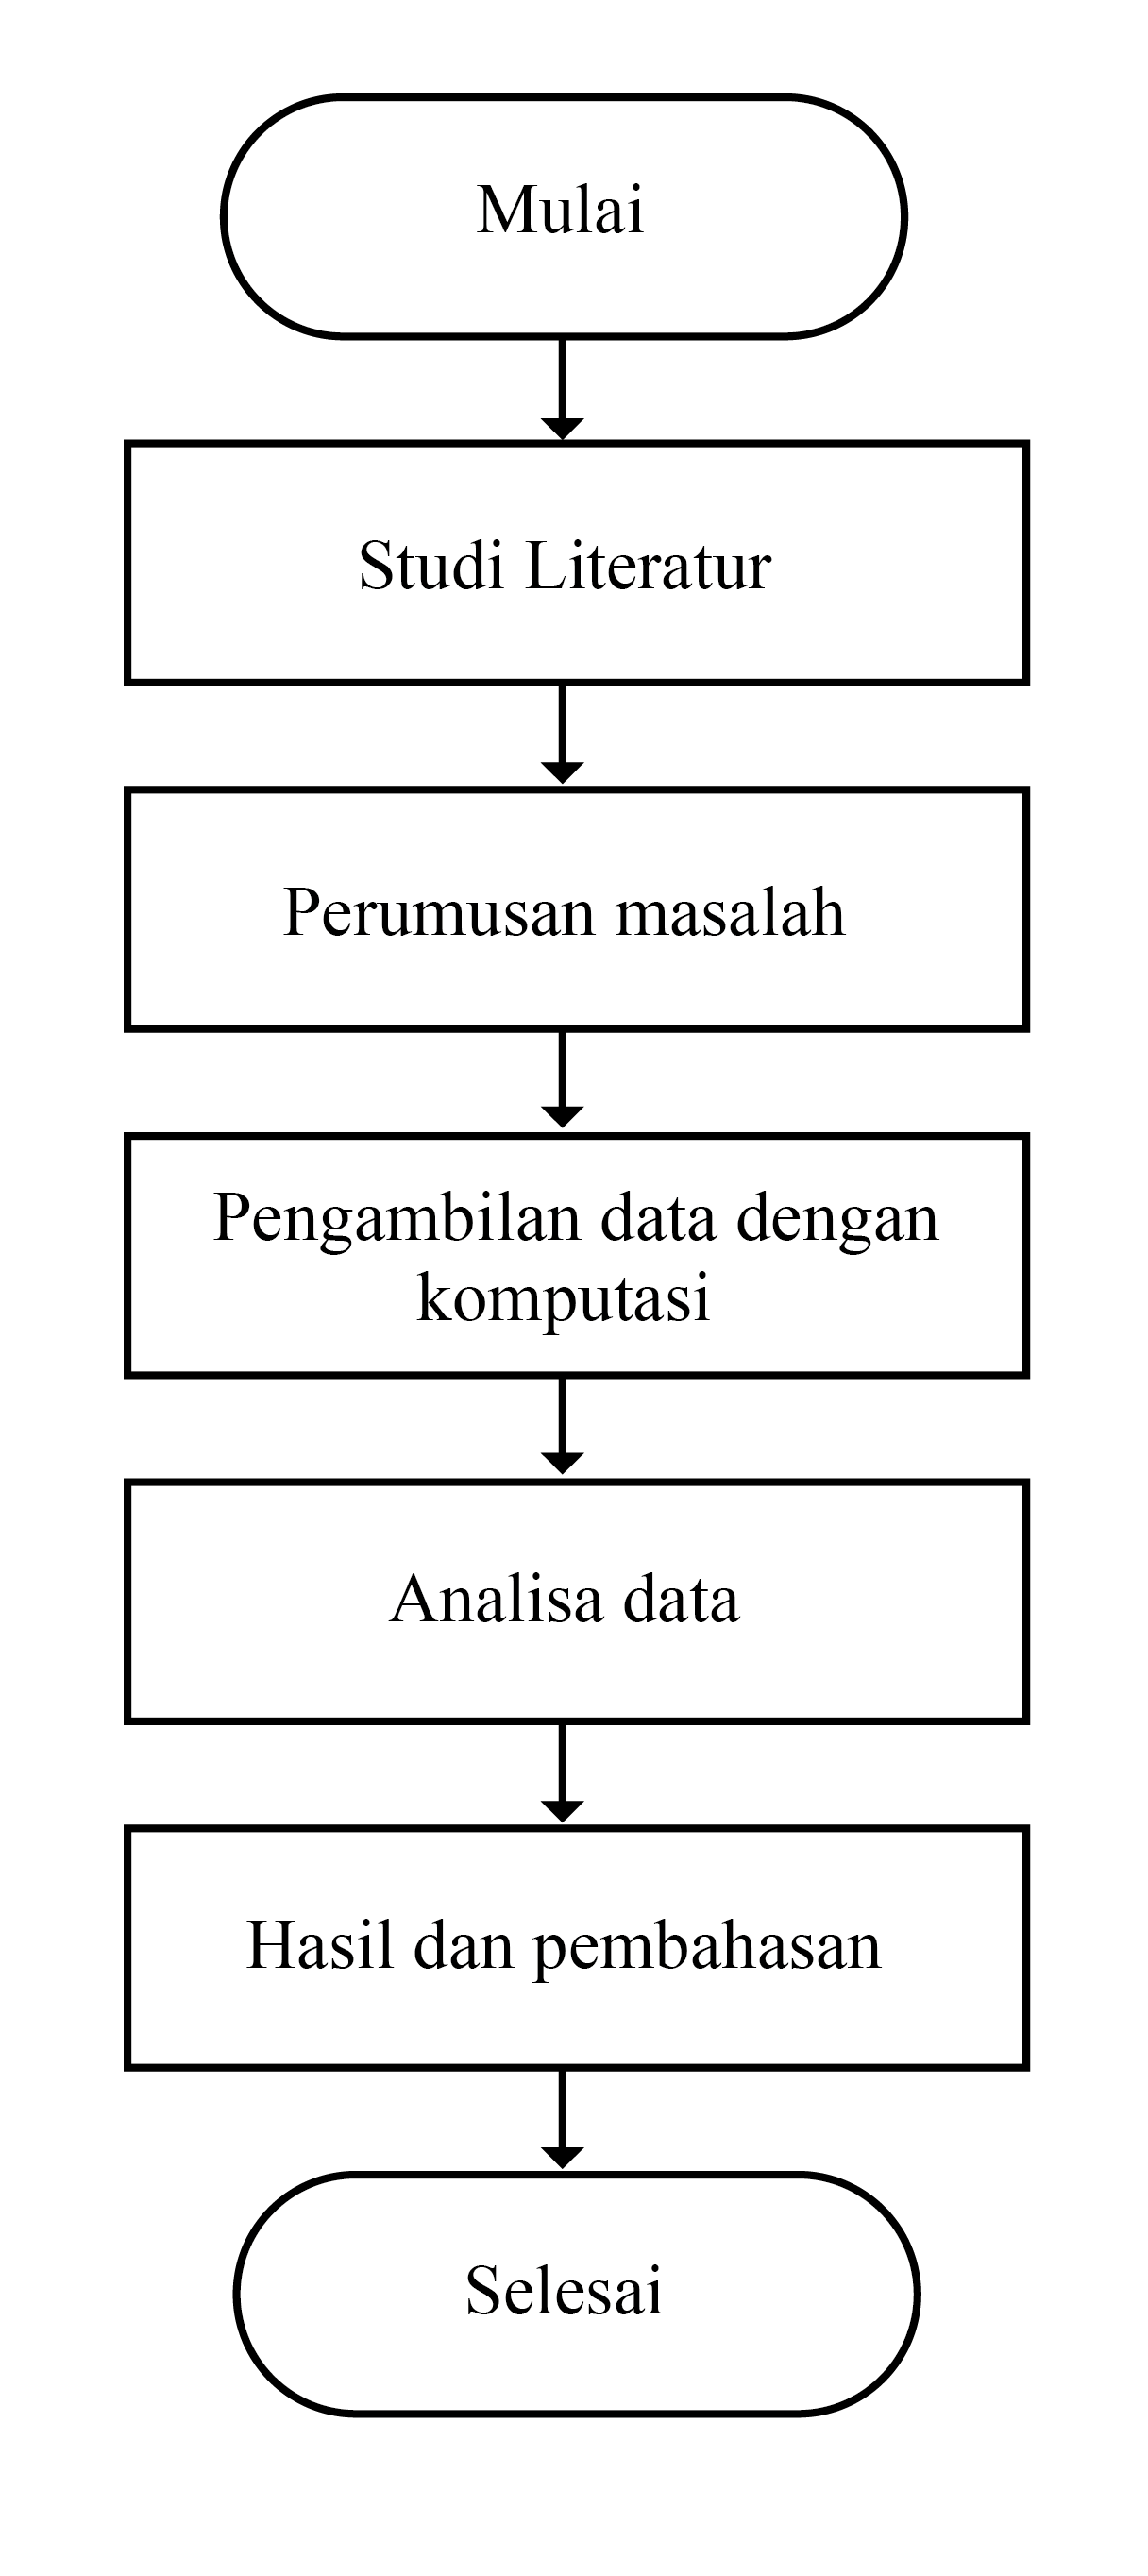
\includegraphics[width=5cm]{gambar/Flowchart Kegiatan.png}
    \caption{Diagram Alir Penelitian}
\end{figure}

%=====================================================================
\section{Jenis dan Desain Penelitian}
%=====================================================================
Pada penelitian ini, jenis penelitian yang digunakan adalah penelitian komputasi, yaitu penelitian yang dilakukan di dalam komputer dengan metode pemodelan mekanika dinamika molekular (MD) dan \textit{ab-initio calculation} untuk menyelidiki sifat elektronik pada struktur material Boron Nitride Heksagonal (hBN) akibat pengaruh suhu menggunakan perangkat lunak LAMMPS dan Quantum ESPRESSO. \section{Rencana Penelitian }

Penelitian ini bertujuan untuk mempelajari sifat elektronik dan magnetik dari hBN sheet 2D single layer dengan dimensi 4x4x1. Struktur hBN disiapkan dan divalidasi melalui studi literatur serta simulasi awal. Selanjutnya, struktur dipanaskan menggunakan LAMMPS guna mencapai kondisi termal optimal, dan hasil pemanasan dianalisis dengan Quantum ESPRESSO untuk mendapatkan informasi mengenai perubahan sifat elektroniknya. Berikut adalah rencana kegiatan penelitian yang berlangsung selama 6 bulan:

\bigskip

\begin{figure}[htbp]
\centering  
\begin{ganttchart}[
    hgrid,
    vgrid,
    title height=1,
    x unit =1cm,
    bar/.style={fill=blue!50},
    milestone/.style={fill=red}
]{1}{6}  % Skala waktu: bulan 1 sampai 6
  % Baris judul untuk bulan
  \gantttitle{\textbf{Bulan}}{6} \\
  \gantttitle{\mbox{Jan}}{1}
  \gantttitle{\mbox{Feb}}{1}
  \gantttitle{\mbox{Mar}}{1}
  \gantttitle{\mbox{Apr}}{1}
  \gantttitle{\mbox{Mei}}{1}
  \gantttitle{\mbox{Jun}}{1} \\
  % Kegiatan penelitian
  \ganttbar{Studi Literatur \& Persiapan Model}{1}{1} \\
  \ganttbar{Persiapan Proposal}{1}{2}\\
  \ganttbar{Simulasi Pemanasan (LAMMPS)}{2}{3} \\
  \ganttbar{Pengumpulan Proposal}{3}{3}\\
  \ganttbar{Analisis Struktur (Quantum ESPRESSO)}{4}{4} \\
  \ganttbar{Penyusunan Laporan}{5}{5} 
 \\
  \ganttbar{Revisi dan Finalisasi Laporan}{6}{6}
\end{ganttchart}
\caption{Gantt Chart Rencana Penelitian Sifat Elektronik hBN Sheet 2D.}
\label{fig:gantt}
\end{figure}

\bigskip

%---------------------------------------------------------------------
\section{Perangkat Penelitian}
%---------------------------------------------------------------------
Dalam prosedur penelitian ini, kami secara komprehensif membahas perangkat dan metodologi yang digunakan untuk menganalisis sifat elektronik lembaran \textit{hexagonal boron nitride} (hBN) 2D yang telah dipanaskan. Penelitian ini dilakukan melalui dua tahap utama, yaitu simulasi dinamika molekul (MD) menggunakan LAMMPS untuk memodelkan evolusi struktur hBN pada rentang suhu 500K hingga 4000K, serta perhitungan teori fungsional kerapatan (DFT) menggunakan Quantum ESPRESSO untuk mengevaluasi perubahan sifat elektronik setelah pemanasan. Pada tahap awal, kami memberikan gambaran tentang perangkat keras dan perangkat lunak yang digunakan, termasuk spesifikasi sistem komputasi berperforma tinggi yang mendukung simulasi dan analisis data. Proses pembuatan dan optimasi struktur hBN dilakukan dengan \textit{Atomic Simulation Environment} (ASE), diikuti dengan simulasi pemanasan menggunakan potensial ReaxFF dalam LAMMPS. Selama simulasi MD, parameter seperti \textit{Radial Distribution Function} (RDF) dan \textit{Mean Squared Displacement} (MSD) dikumpulkan untuk memantau perubahan struktur dan dinamika atom. Setelah simulasi MD, struktur akhir dikonversi ke format yang kompatibel dengan Quantum ESPRESSO untuk perhitungan DFT lebih lanjut. Proses ini melibatkan perhitungan \textit{Self-Consistent Field} (SCF) untuk mendapatkan kerapatan muatan yang stabil, diikuti dengan \textit{Non-Self-Consistent Field} (NSCF) untuk menghitung struktur pita elektronik, \textit{Density of States} (DOS), \textit{Projected Density of States} (PDOS), serta distribusi muatan (\textit{charge density}). Seluruh perhitungan dilakukan dengan pendekatan spin-polarized menggunakan fungsi pertukaran-korelasi PBEsol PAW. Untuk memahami perubahan sifat elektronik akibat pemanasan, hasil perhitungan DFT divisualisasikan dan dianalisis menggunakan OVITO, VMD, XCrySDen, dan VESTA, sementara pemrosesan data numerik dilakukan dengan NumPy, Matplotlib, dan Seaborn. Dengan dokumentasi prosedur yang jelas dan parameter yang terperinci, penelitian ini diharapkan dapat memberikan wawasan mendalam tentang pengaruh suhu terhadap sifat elektronik hBN serta memungkinkan replikasi dan validasi oleh penelitian lain. \section{Perangkat Penelitian}
Dalam penelitian ini, perangkat penelitian terdiri dari perangkat keras dan perangkat lunak yang digunakan untuk mendukung simulasi dan analisis sifat elektronik dari struktur lembaran \textit{hexagonal boron nitride} (hBN) 2D setelah pemanasan. Kombinasi perangkat keras berperforma tinggi dan perangkat lunak komputasi canggih memungkinkan penelitian ini dilakukan secara efisien dan akurat. \subsection{Perangkat Keras}
Penelitian ini dilakukan pada sistem komputasi dengan spesifikasi sebagai berikut:
\begin{enumerate}
    \item 3 node komputasi. \item Setiap node memiliki 1x AMD EPYC 7702P, dengan 64 core / 128 thread, kecepatan 2.0 GHz. \item RAM sebesar 240 GB.
    \item Interkoneksi menggunakan Mellanox RoCE 100Gbps. \end{enumerate}

\subsection{Perangkat Lunak}
Penelitian ini menggunakan berbagai perangkat lunak untuk mendukung simulasi dan analisis data. Quantum ESPRESSO digunakan sebagai perangkat lunak utama dalam perhitungan DFT, memungkinkan evaluasi struktur elektronik material dengan pendekatan \textit{plane-wave pseudopotential}. LAMMPS digunakan untuk simulasi dinamika molekul (MD), di mana interaksi antar-atom dimodelkan menggunakan potensial ReaxFF untuk memahami efek pemanasan pada struktur hBN. Untuk visualisasi hasil simulasi dan analisis struktur, berbagai perangkat lunak digunakan, termasuk VMD, OVITO, XCrySDen, dan VESTA. VMD digunakan untuk menampilkan dinamika atom secara real-time dalam simulasi MD, sementara OVITO menyediakan alat analisis struktur kristal yang lebih fleksibel. XCrySDen membantu dalam visualisasi struktur elektronik dari hasil perhitungan Quantum ESPRESSO, dan VESTA digunakan untuk menampilkan distribusi kerapatan muatan serta struktur pita elektronik. Pembuatan dan manipulasi struktur kristal dilakukan menggunakan \textit{Atomic Simulation Environment} (ASE), yang memungkinkan konversi format dan pembuatan model supercell. Untuk analisis dan pemrosesan data numerik, NumPy digunakan sebagai pustaka utama untuk komputasi numerik, sedangkan Matplotlib dan Seaborn digunakan untuk memvisualisasikan hasil analisis seperti \textit{Radial Distribution Function} (RDF), \textit{Mean Squared Displacement} (MSD), serta data dari perhitungan DFT seperti \textit{Density of States} (DOS) dan \textit{Projected Density of States} (PDOS). Seluruh proses analisis dan pengolahan data dilakukan dalam lingkungan Jupyter Notebook untuk kemudahan dokumentasi dan reprodusibilitas penelitian. %---------------------------------------------------------------------
\section{Prosedur Penelitian}
Dalam prosedur penelitian ini, kami secara komprehensif membahas perangkat dan metodologi yang digunakan untuk menganalisis sifat elektronik lembaran \textit{hexagonal boron nitride} (hBN) 2D yang telah dipanaskan. Penelitian ini dilakukan melalui dua tahap utama, yaitu simulasi dinamika molekul (MD) menggunakan LAMMPS untuk memodelkan evolusi struktur hBN pada rentang suhu 500K hingga 4000K, serta perhitungan teori fungsional kerapatan (DFT) menggunakan Quantum ESPRESSO untuk mengevaluasi perubahan sifat elektronik setelah pemanasan. Pada tahap awal, kami memberikan gambaran tentang perangkat keras dan perangkat lunak yang digunakan, termasuk spesifikasi sistem komputasi berperforma tinggi yang mendukung simulasi dan analisis data. Proses pembuatan dan optimasi struktur hBN dilakukan dengan \textit{Atomic Simulation Environment} (ASE), diikuti dengan simulasi pemanasan menggunakan potensial ReaxFF dalam LAMMPS. Selama simulasi MD, parameter seperti \textit{Radial Distribution Function} (RDF) dan \textit{Mean Squared Displacement} (MSD) dianalisis untuk memahami perubahan struktur akibat pemanasan. Setelah simulasi MD, struktur akhir dikonversi ke format yang kompatibel dengan Quantum ESPRESSO untuk perhitungan DFT lebih lanjut. Proses ini melibatkan perhitungan \textit{Self-Consistent Field} (SCF) untuk mendapatkan kerapatan muatan yang stabil, diikuti dengan \textit{Non-Self-Consistent Field} (NSCF) untuk menghitung struktur pita elektronik, \textit{Density of States} (DOS), \textit{Projected Density of States} (PDOS), serta distribusi muatan (\textit{charge density}). Seluruh perhitungan dilakukan dengan pendekatan spin-polarized menggunakan fungsi pertukaran-korelasi PBEsol PAW. Untuk memahami perubahan sifat elektronik akibat pemanasan, hasil perhitungan DFT divisualisasikan dan dianalisis menggunakan OVITO, VMD, XCrySDen, dan VESTA, sementara pemrosesan data numerik dilakukan dengan NumPy, Matplotlib, dan Seaborn. Dengan dokumentasi prosedur yang jelas dan parameter yang terperinci, penelitian ini diharapkan dapat memberikan wawasan mendalam tentang pengaruh suhu terhadap sifat elektronik hBN serta memungkinkan replikasi dan validasi oleh penelitian lain. \vspace{3mm}

\begin{figure}
    \centering
    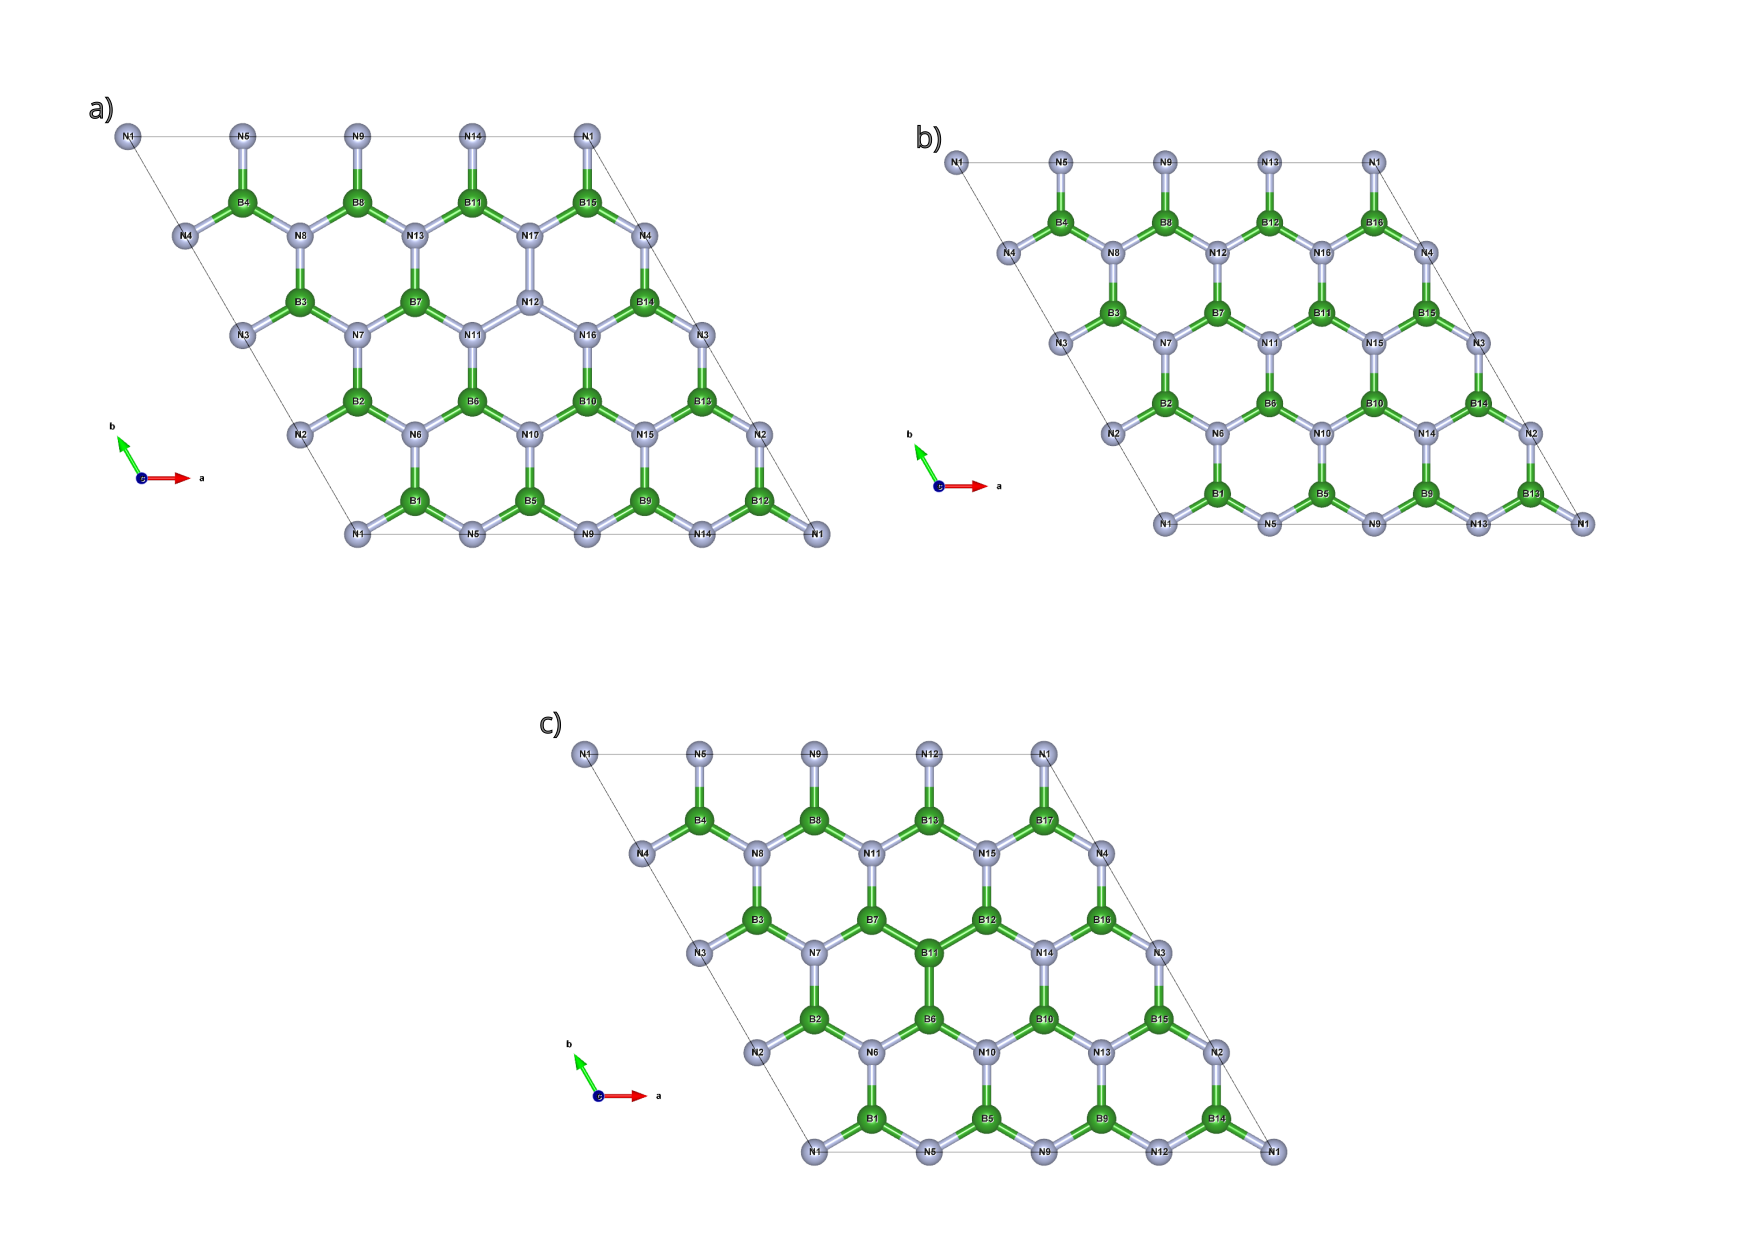
\includegraphics[width=0.8\linewidth]{gambar_hasil/structures_all.png}
    \caption{Model hBN 4x4x1 dengan a) struktur hBN murni b) struktur hBN dengan cacat N-N c) struktur hBN dengan cacat B-B}
    \label{Struktur hBN 4x4x1}
\end{figure}

\subsection{Detail Komputasi}
Dalam penelitian ini digunakan Quantum ESPRESSO \citep{Giannozzi2009} dan LAMMPS \citep{Plimpton1995} sebagai perangkat lunak komputasi. Digunakan supersel 4x4x1 untuk membentuk struktur \textit{hBN} yang dapat dilihat di Gambar 3.3 Kalkulasi dengan LAMMPS menggunakan variasi potensial ReaxFF \citep{Lele2022} dan ensemble NVT dengan pemanasan dari rentang temperatur 500K hingga 4000K. Pada kalkulasi dengan Quantum ESPRESSO digunakan variasi \texttt{ecutwfc} sebesar 60 Ry dan \texttt{K-POINTS} sebesar $8\times8\times1$ untuk membagi daerah Brillouin dengan kisi Monkhorst-Pack (MP) \citep{Monkhorst1976}. Kedua nilai tersebut diperoleh dari uji konvergensi yang akan dijelaskan lebih lengkap pada BAB 4. Digunakan fungsional Perdew-Burke-Ernzerhof (PBE) \citep{Perdew1996} sebagai \textit{generalized gradient approximation} (GGA) untuk melengkapi fungsi korelasi dan pertukaran. Potensial semu yang digunakan untuk menggambarkan elektron valensi dan elektron inti adalah \textit{projector augmented wave method} (PAW) \citep{Blochl1994}. Selain itu, ruang vakum dibuat sebesar 20\AA.
Diagram alir komputasi yang akan dilakukan dalam penelitian ini dapat dilihat pada Gambar 3.5 dan Gambar 3.6. Seluruh prosedur komputasi dalam Gambar 3.5 dilakukan untuk komputasi menggunakan MD sedangkan Gambar 3.6 untuk komputasi menggunakan DFT. Sementara visualisasi data hasil komputasi dibuat dengan bantuan dari kode Python menggunakan library Matplotlib dan NumPy yang dibuat di dalam VS Code dengan Jupyter Notebook. \begin{figure}
    \centering
    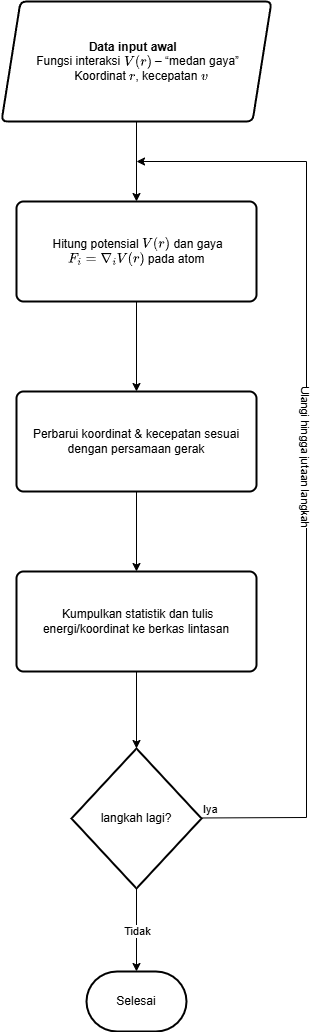
\includegraphics[width=0.35\linewidth]{gambar/MD.drawio.png}
    \caption{Alur Komputasi MD}
    \label{Diagram Alir MD}
\end{figure}

\begin{figure}
    \centering
    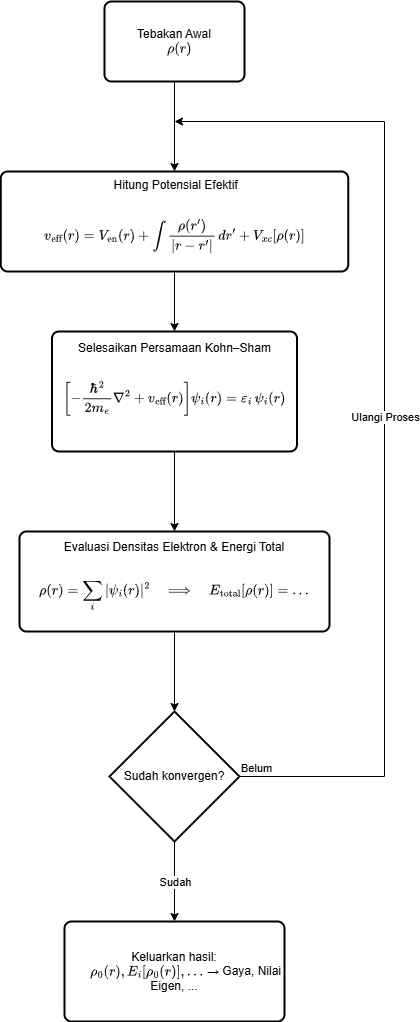
\includegraphics[width=0.5\linewidth]{gambar/DFT.drawio.png}
    \caption{Alur Komputasi DFT }
    \label{Diagram Alir DFT}
\end{figure}

\subsection{Langkah Kerja}
\label{sec:intro}
Penelitian ini bertujuan untuk mengkaji sifat elektronik lembaran \textit{hexagonal boron nitride} (hBN) 2D lapisan tunggal berukuran 4×4×1. Metodologi yang digunakan meliputi simulasi dinamika molekul (MD) dengan LAMMPS dan perhitungan teori fungsional kerapatan (DFT) dengan Quantum ESPRESSO. Visualisasi dan analisis data dilakukan menggunakan OVITO, VMD, XCrySDen, VESTA, serta pustaka Python seperti NumPy, Matplotlib, dan Seaborn. \subsubsection*{Pembuatan dan Relaksasi Struktur Awal hBN}
\label{sec:structure}
\begin{enumerate}
    \item \textbf{Pembuatan Struktur:} Struktur awal hBN 2D lapisan tunggal dengan ukuran 4×4×1 dibuat menggunakan \textit{Atomic Simulation Environment} (ASE). Struktur ini kemudian disimpan dalam format yang kompatibel dengan LAMMPS, seperti file data. \item \textbf{Relaksasi Struktur:} Struktur awal direlaksasi menggunakan LAMMPS dengan potensial ReaxFF khusus untuk hBN. \textit{Time Step} (TS) yang digunakan adalah 0,25 fs. Relaksasi dilakukan hingga gaya antar atom mencapai nilai di bawah 0,01 eV/Å, memastikan struktur berada pada kondisi energi minimum. \end{enumerate}

\subsubsection*{Simulasi Pemanasan dengan MD}
\label{sec:md_simulation}
\begin{enumerate}
    \item \textbf{Proses Pemanasan:} Setelah relaksasi, struktur dipanaskan secara bertahap dari 500K hingga 4000K menggunakan LAMMPS dengan \textit{Time Step} (TS) 0,25 fs. Pemanasan bertahap ini penting untuk menghindari guncangan termal yang dapat menyebabkan ketidakstabilan struktur. \item \textbf{Pengumpulan Data:} Selama simulasi, data seperti \textit{Radial Distribution Function} (RDF) dan \textit{Mean Squared Displacement} (MSD) dikumpulkan untuk memantau perubahan struktur dan dinamika atom. \end{enumerate}

\subsubsection*{Konversi Struktur untuk Perhitungan DFT}
\label{sec:structure_conversion}
Struktur akhir dari simulasi MD diekstraksi dan dikonversi ke format input yang kompatibel dengan Quantum ESPRESSO menggunakan ASE. Konversi ini memastikan tidak ada kehilangan informasi geometri dan gaya residu tetap minimal, sehingga struktur siap untuk perhitungan DFT. \subsubsection*{Perhitungan DFT: SCF dan NSCF}
\label{sec:dft_calculations}
\begin{enumerate}
    \item \textbf{Perhitungan SCF:} Langkah pertama dalam perhitungan DFT adalah melakukan perhitungan \textit{Self-Consistent Field} (SCF) untuk memperoleh distribusi kerapatan muatan yang konsisten dengan potensial yang dihasilkannya. Parameter seperti energi cutoff dan kisi k-point diatur untuk mencapai konvergensi yang baik. \item \textbf{Perhitungan NSCF:} Setelah perhitungan SCF, dilakukan perhitungan \textit{Non-Self-Consistent Field} (NSCF) menggunakan kerapatan muatan yang telah diperoleh. NSCF biasanya dilakukan dengan grid k-point yang lebih rapat atau sepanjang jalur simetri tinggi dalam zona Brillouin. Langkah ini penting untuk menghitung energi eigen secara akurat guna analisis struktur pita dan \textit{Density of States} (DOS). \end{enumerate}

\subsubsection*{Perhitungan Sifat Elektronik dengan Spin Terpolarisasi}
\label{sec:electronic_properties}
Setelah perhitungan NSCF, perhitungan sifat elektronik dilakukan dengan mempertimbangkan polaritas spin. Analisis meliputi:
\begin{enumerate}
    \item \textbf{Struktur Pita (Band Structure, BS):} Menunjukkan hubungan antara energi dan momentum elektron, memberikan informasi tentang sifat konduktif atau isolatif material. \item \textbf{Density of States (DOS):} Menggambarkan jumlah keadaan elektron yang tersedia pada tiap tingkat energi. \item \textbf{Projected Density of States (PDOS):} Menjelaskan kontribusi masing-masing orbital atomik terhadap DOS total. \item \textbf{Kerapatan Muatan (Charge Density):} Menunjukkan distribusi elektron dalam material, penting untuk memahami karakter ikatan kimia.
\end{enumerate}
    %%%%%%%%%%%%%%%%%%%%%%%%%%%%%%%%%%%%%%%%%%%%%%%%%%%%%%%%%%%%%%%%%%%%%%
% CATATAN: Kode ini mengasumsikan bahwa paket-paket berikut telah dimuat
% di dokumen utama Anda (preamble):
% \usepackage{graphicx}
% \usepackage{booktabs}
% \usepackage{amsmath}
% \usepackage{subcaption} % Paket krusial untuk lingkungan subfigure
% \usepackage{hyperref}   % Untuk referensi yang dapat diklik
%%%%%%%%%%%%%%%%%%%%%%%%%%%%%%%%%%%%%%%%%%%%%%%%%%%%%%%%%%%%%%%%%%%%%%

\newpage
%%%%%%%%%%%%%%%%%%%%%%%%%%%%%%%%%%%%%%%%%%%%%%%%%%%%%%%%%%%%%%%%%%%%%%
% BAB HASIL DAN PEMBAHASAN:
%=====================================================================
\renewcommand{\thechapter}{\Roman{chapter}}
\addtocontents{toc}{\vskip10pt}
\chapter{HASIL DAN PEMBAHASAN}
\renewcommand{\thechapter}{\arabic{chapter}}
%---------------------------------------------------------------------

\section{Tinjauan Metodologi Komputasi dan Implikasinya pada Hasil}
\label{sec:metodologi_kritis}
Keandalan prediksi dalam pemodelan material pada skala atomistik sangat bergantung pada pemilihan metodologi komputasi yang tepat dan pemahaman mendalam tentang batasan inherennya.
Bagian ini menyajikan tinjauan metodologis terhadap dua pilar komputasi yang digunakan dalam penelitian ini: simulasi Dinamika Molekuler (MD) untuk generasi struktur termal dan Teori Fungsional Kerapatan (DFT) untuk kalkulasi sifat elektronik.
Evaluasi ini krusial karena kualitas struktur atomik input dan pilihan parameter kuantum secara fundamental menentukan akurasi serta validitas interpretasi hasil akhir.
\subsection{Generasi Struktur melalui Dinamika Molekuler: Potensial ReaxFF}
\label{subsec:md_reaxff}
Struktur atomik yang merepresentasikan monolayer hBN pada temperatur tinggi (800 K, 1100 K, dan 1225 K) dihasilkan melalui simulasi dinamika molekuler (MD) menggunakan perangkat lunak LAMMPS \citep{Plimpton1995}.
Interaksi antar-atom dimodelkan menggunakan potensial medan gaya reaktif (ReaxFF), dengan parameterisasi yang dikembangkan oleh Lele et al. \citep{Lele2022}.
Pemilihan potensial interatomik merupakan langkah kritis yang menentukan evolusi sistem dan konfigurasi kesetimbangan termalnya.
Potensial ReaxFF, pada dasarnya, dirancang untuk memodelkan proses kimia yang kompleks, di mana pembentukan dan pemutusan ikatan menjadi fenomena sentral.
Hal ini dicapai melalui konsep orde ikatan yang dinamis, yang memungkinkan deskripsi jalur reaksi secara akurat \citep{Weismiller2010, vanDuin2001, Senftle2016}.
Parameterisasi spesifik yang digunakan dalam penelitian ini \citep{Lele2022} dioptimalkan untuk mereplikasi kimia fasa gas yang relevan dengan sintesis nanostruktur hBN, seperti pada proses \emph{Chemical Vapor Deposition} (CVD).
Meskipun sangat kuat dalam domainnya, penting untuk mengenali bahwa potensial yang dioptimalkan untuk dinamika reaksi belum tentu ideal untuk mereproduksi sifat-sifat fasa padat yang lebih subtil, seperti spektrum fonon atau respons termomekanik yang halus \citep{Fthenakis2022, Deringer2020}.
Studi komparatif menunjukkan bahwa beberapa parameterisasi ReaxFF dapat menunjukkan keterbatasan dalam memprediksi modulus elastisitas atau spektrum fonon secara kuantitatif untuk material berbasis $\emph{sp}^2$ \citep{Fthenakis2022, Deringer2020}.
Implikasi paling signifikan untuk penelitian ini adalah potensi kegagalan ReaxFF dalam menangkap fisika anharmonik dari moda fonon lentur (\emph{flexural phonons}).
Pada material 2D seperti hBN dan grafena, eksitasi termal dari moda vibrasi keluar-bidang (dikenal sebagai moda ZA) dapat menyebabkan fenomena Ekspansi Termal Negatif (NTE), di mana kisi mengalami kontraksi saat dipanaskan \citep{Sarikurt2022, Mann2017}.
Mekanisme ini, yang dikenal sebagai efek membran \citep{Yates1972}, sangat bergantung pada deskripsi yang sangat presisi dari anharmonisitas potensial.
Mengingat fokus parameterisasi ReaxFF yang digunakan adalah pada energi reaksi fasa gas \citep{Lele2022}, kemungkinan besar potensial ini tidak mereproduksi perilaku moda ZA secara akurat.
Konsekuensinya, struktur yang dihasilkan MD mungkin tidak menunjukkan kontraksi kisi yang diharapkan, sebuah poin penting yang akan dibahas lebih lanjut saat menganalisis ketergantungan temperatur dari celah pita pada Bagian \ref{subsec:hbn_murni_termal}.
Oleh karena itu, hasil yang diperoleh harus diinterpretasikan sebagai representasi sistem di bawah asumsi yang ditentukan oleh medan gaya yang dipilih, di mana efek termal didominasi oleh mekanisme selain NTE.
\subsection{Kalkulasi Sifat Elektronik: Fungsional PBEsol dan Keterbatasannya}
\label{subsec:dft_qe}
Setelah struktur atomik diperoleh, sifat elektronik dihitung menggunakan Teori Fungsional Kerapatan (DFT) \citep{Hohenberg1964, Kohn1965} dalam paket perangkat lunak Quantum ESPRESSO \citep{Giannozzi2009, Giannozzi2017}.
Fungsional tukar-tambah-korelasi yang digunakan adalah Perdew-Burke-Ernzerhof yang dioptimalkan untuk padatan (PBEsol) \citep{Perdew2008}.
PBEsol, sebagai bagian dari kerangka Aproksimasi Gradien Umum (GGA), dirancang untuk memberikan deskripsi yang lebih baik tentang tumpang-tindih kerapatan elektron dalam padatan, yang seringkali menghasilkan parameter kisi yang lebih akurat dibandingkan PBE standar \citep{Perdew2008}.
Namun, seperti semua fungsional (semi-)lokal, PBEsol memiliki keterbatasan sistematis dalam memprediksi celah pita energi ($E_g$) semikonduktor dan isolator, di mana ia cenderung meremehkan (\emph{underestimate}) nilai tersebut secara signifikan \citep{perdew2005}.
Untuk hBN, nilai celah pita eksperimental dilaporkan berada di kisaran 5.9–6.1 eV \citep{Watanabe2004, Elias2019}, sementara kalkulasi PBE/PBEsol umumnya menghasilkan nilai 4.5–4.7 eV.
Hasil yang diperoleh dalam penelitian ini untuk hBN murni, $E_g = 4.446$ eV, konsisten dengan tingkat penyusutan ini.
Penyebab fundamental dari peremehan celah pita ini adalah Kesalahan Interaksi-Diri atau \emph{Self-Interaction Error} (SIE) \citep{perdew1981}.
Dalam teori yang eksak, energi tukar harus secara sempurna membatalkan energi elektrostatis Hartree dari interaksi sebuah elektron dengan dirinya sendiri.
Fungsional aproksimasi seperti GGA gagal mencapai pembatalan sempurna ini, menyebabkan setiap elektron secara artifisial "merasakan" tolakan dari sebagian densitas muatannya sendiri \citep{MoriSanchez2008}.
Konsekuensi utama dari SIE adalah kecenderungan fungsional untuk secara tidak fisik menyukai keadaan elektronik yang terdelokalisasi, karena ini menyebarkan kerapatan muatan dan mengurangi energi interaksi-diri palsu.
Pada hBN, di mana puncak pita valensi (VBM) didominasi oleh orbital N $2p$ yang relatif terlokalisasi, SIE menyebabkan orbital-orbital ini menjadi terlalu terdelokalisasi, yang secara artifisial menaikkan energinya.
Kombinasi dari VBM yang dinaikkan dan pita konduksi (CBM) yang diturunkan secara langsung menghasilkan nilai $E_g$ yang lebih kecil dari nilai sebenarnya.
Meskipun terdapat keterbatasan kuantitatif ini, PBEsol tetap merupakan alat yang valid dan andal untuk menganalisis \emph{tren kualitatif} dan \emph{perubahan relatif} pada sifat elektronik.
Selama interpretasi difokuskan pada perbandingan antar sistem (misalnya, murni vs. cacat) atau perubahan sebagai fungsi temperatur, kesimpulan yang ditarik tetap bermakna secara fisik.
Kalkulasi DFT dilakukan pada supercell monolayer hBN berukuran $4 \times 4 \times 1$ (32 atom).
Ukuran ini memadai untuk material murni, namun untuk studi cacat titik, ia dapat menimbulkan efek ukuran terbatas (\emph{finite-size effects}) akibat interaksi artifisial antara cacat dan citra periodiknya.
Interaksi non-fisik ini dapat mempengaruhi akurasi energi pembentukan, posisi tingkat energi cacat, dan terutama sifat magnetik yang mungkin diinduksi \citep{Freysoldt2014}.
Secara khusus, ketika sistem menunjukkan kecenderungan menuju tatanan magnetik, seperti pada kasus cacat B\textsubscript{N}, interaksi pertukaran antar citra periodik dapat secara keliru menstabilkan keadaan magnetik.
Oleh karena itu, sifat-sifat cacat yang diperoleh, khususnya yang berkaitan dengan magnetisme, harus diinterpretasikan dengan mempertimbangkan potensi pengaruh dari ukuran supercell yang digunakan.

\section{Analisis Stabilitas dan Struktur Termal dari Simulasi MD}
\label{sec:analisis_md}
Sebelum menyelidiki sifat elektronik, penting untuk terlebih dahulu memahami bagaimana perlakuan termal dan keberadaan cacat mempengaruhi struktur dan dinamika atomik monolayer hBN.
Analisis ini, yang berasal dari simulasi MD, memberikan fondasi struktural untuk semua kalkulasi DFT berikutnya.
\subsection{Struktur Atomik Hasil Pemanasan}
\label{subsec:md_struktur}
Simulasi MD pada temperatur tinggi menghasilkan struktur yang secara signifikan terdistorsi dari konfigurasi heksagonal datar yang ideal.
Pemanasan menginduksi fluktuasi termal yang menyebabkan atom-atom bergerak keluar dari bidang, menciptakan kerutan atau riak (\emph{rippling}) pada permukaan monolayer.

%%%%%%%%%%%%%%%%%%%%%%%%%%%%%%%%%%%%%%%%%%%%%%%%%%%%%%%%%%%%%%%%%%%%%%
% PERBAIKAN GAMBAR 1: STRUKTUR ATOMIK (Tata Letak Vertikal, Ukuran Maksimal)
% Permintaan: Menyusun gambar secara vertikal, lebih besar, dan membiarkan
% LaTeX memindahkannya ke halaman baru jika perlu.
% Solusi: Setiap kondisi (sistem + temperatur) ditempatkan dalam 'subfigure'
% sendiri yang lebarnya diatur ke \textwidth untuk ukuran maksimal. Di dalamnya,
% gambar tampak atas dan samping ditempatkan berdampingan. Tumpukan vertikal
% ini menciptakan 'figure' yang sangat tinggi.
% Penanganan Halaman: Spesifikasi float [htbp!] memberi tahu LaTeX untuk
% mencoba menempatkan gambar di sini, di atas, di bawah, atau—yang paling
% mungkin untuk gambar setinggi ini—pada halaman khusus float [p]. Ini
% persis sesuai dengan permintaan agar gambar bisa pindah ke halaman selanjutnya.
%%%%%%%%%%%%%%%%%%%%%%%%%%%%%%%%%%%%%%%%%%%%%%%%%%%%%%%%%%%%%%%%%%%%%%
% --- Bagian 1: Sistem Murni ---
\begin{figure}[htbp]
  \centering
  \begin{subfigure}{\textwidth}
    \centering
    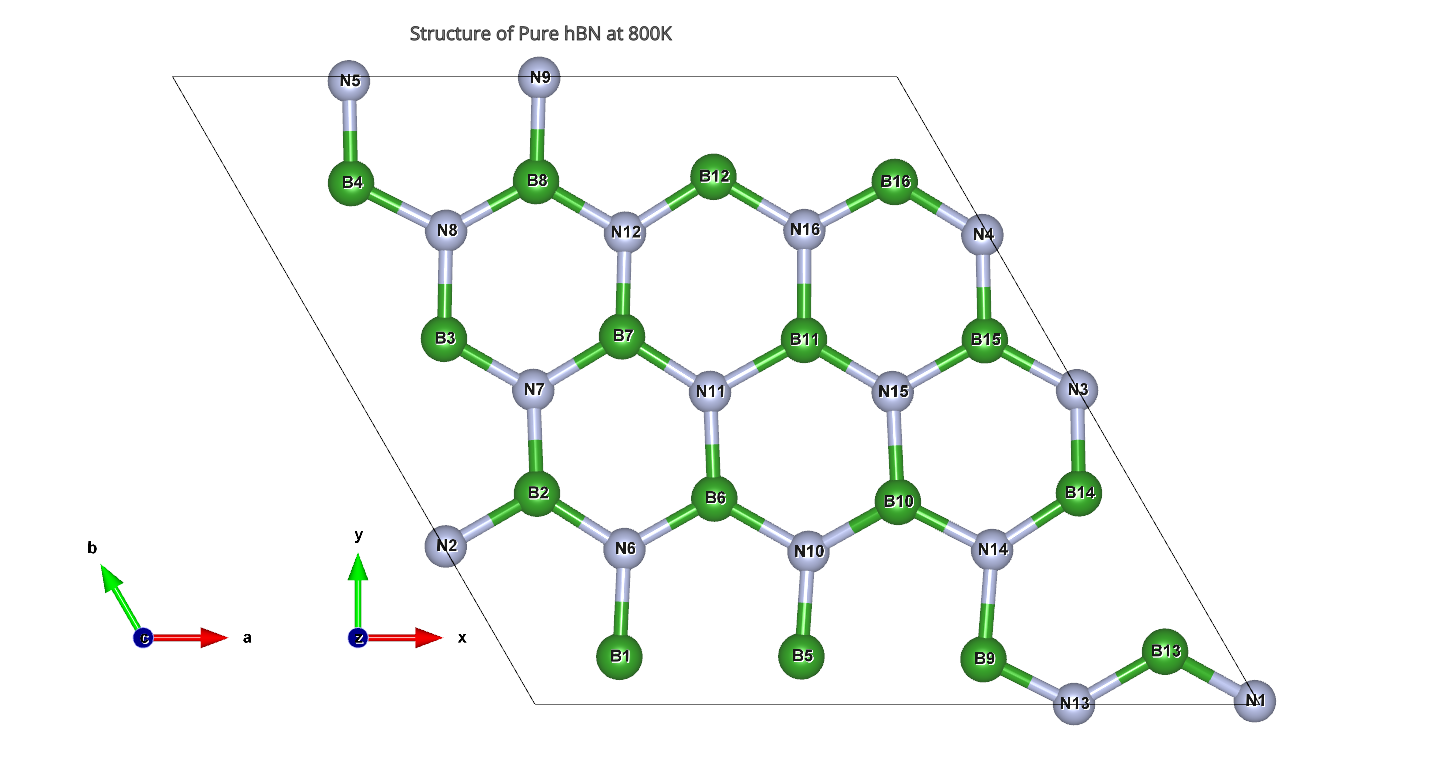
\includegraphics[width=0.49\linewidth]{gambar_hasil/hBN_pure_800K.png}\hfill
    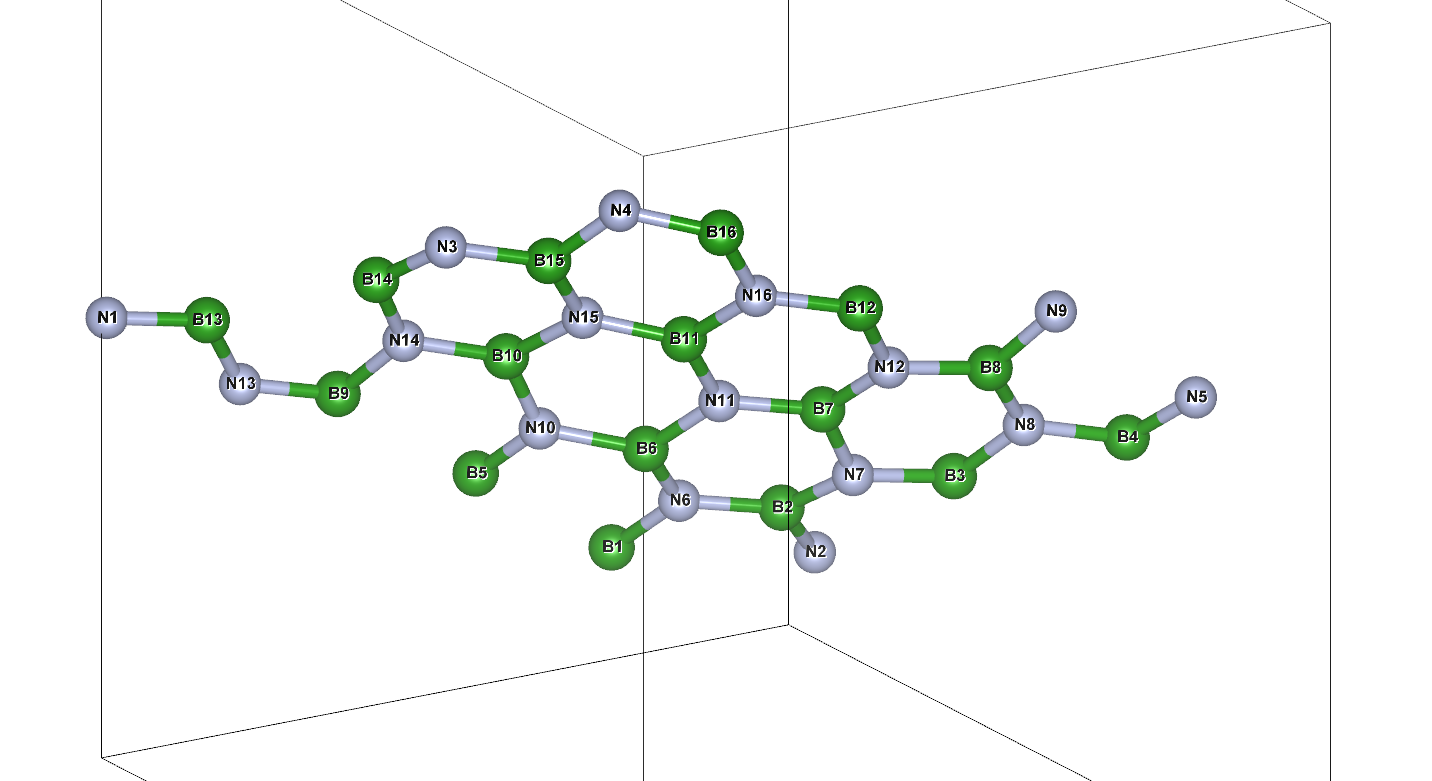
\includegraphics[width=0.49\linewidth]{gambar_hasil/hBN_pure_side_800K.png}
    \caption{Murni, 800 K}
    \label{subfig:md_pure_800k}
  \end{subfigure}
  \vspace{1em}
  \begin{subfigure}{\textwidth}
    \centering
    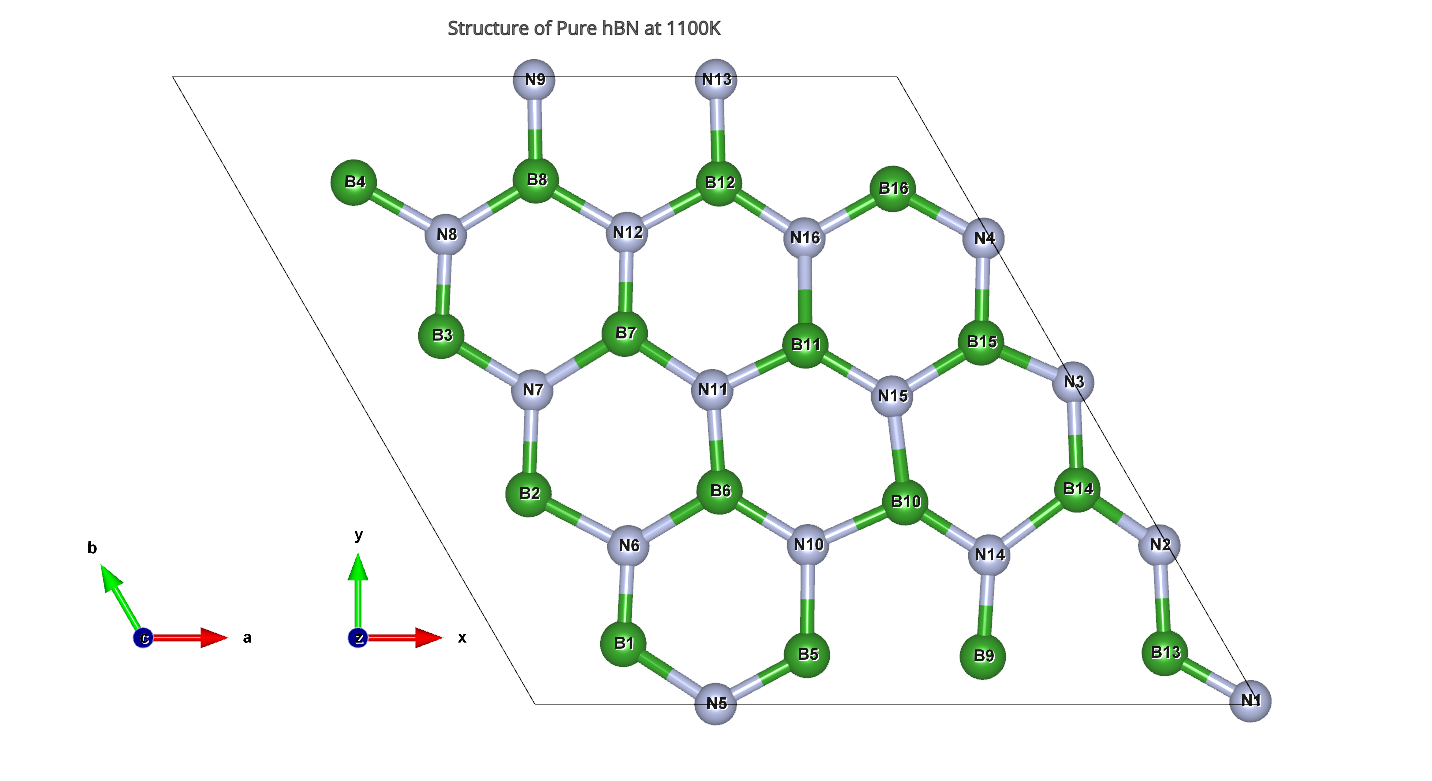
\includegraphics[width=0.49\linewidth]{gambar_hasil/hBN_pure_1100K.png}\hfill
    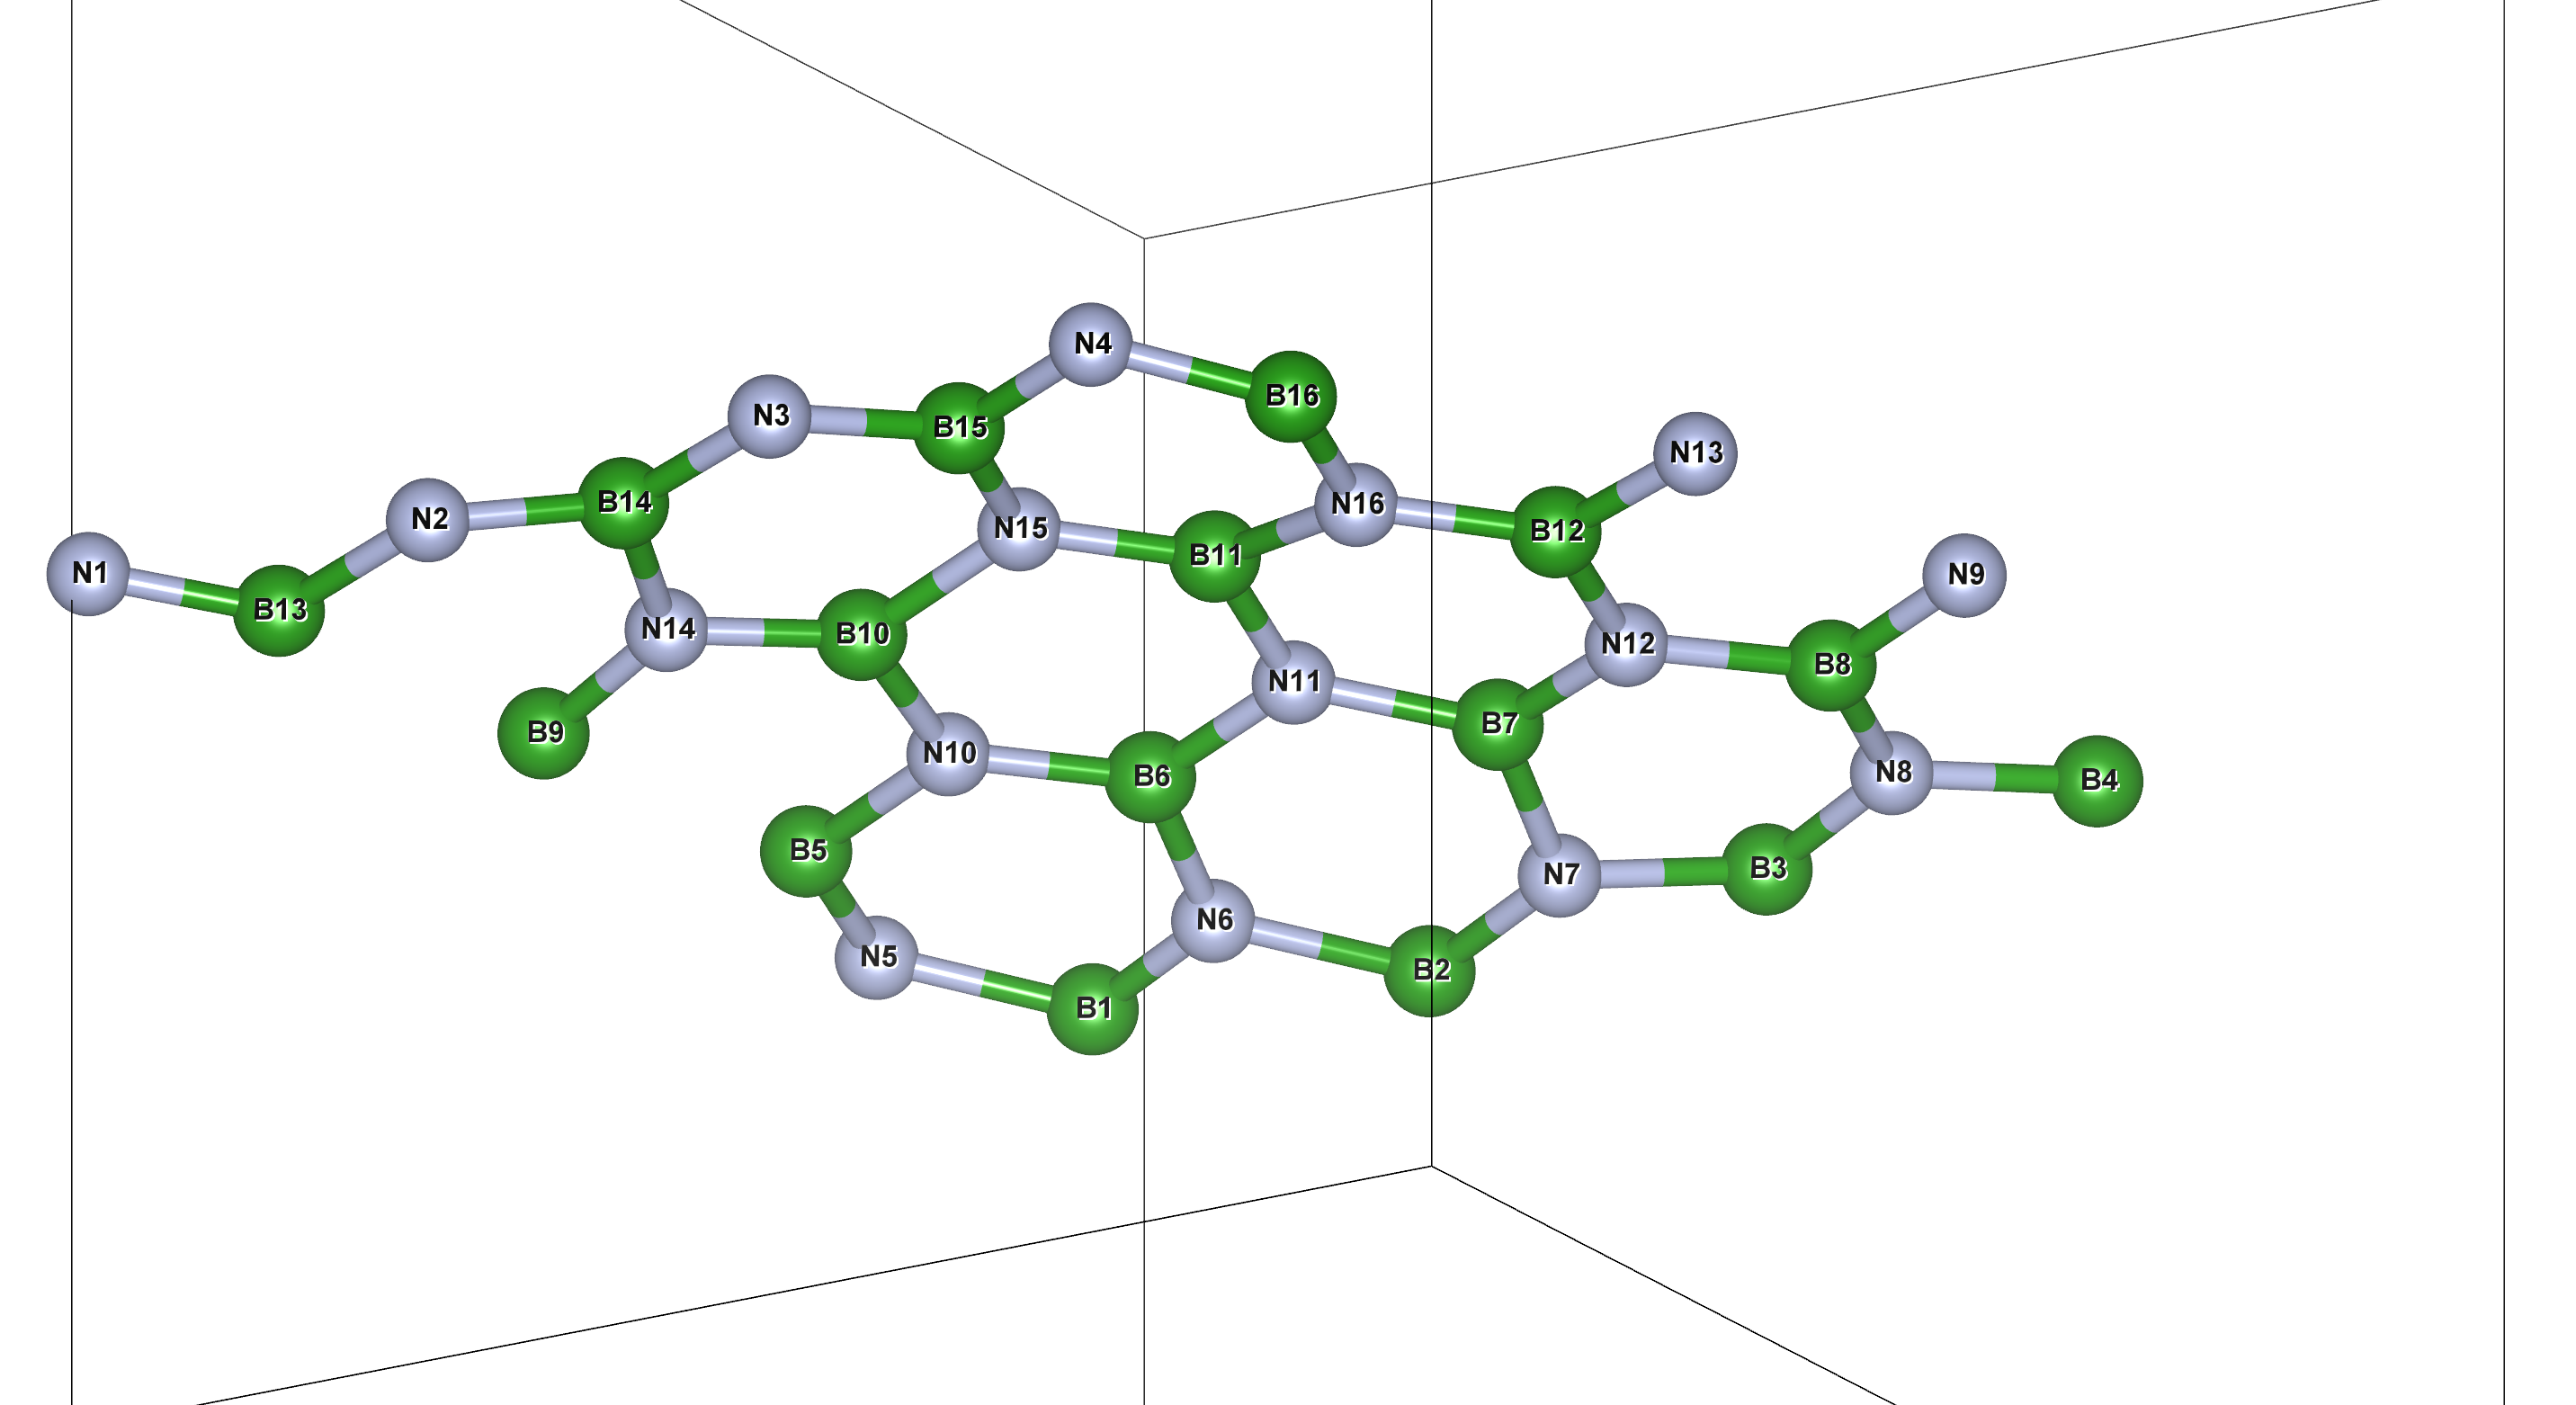
\includegraphics[width=0.49\linewidth]{gambar_hasil/hBN_pure_side_1100K.png}
    \caption{Murni, 1100 K}
    \label{subfig:md_pure_1100k}
  \end{subfigure}
  \vspace{1em}
  \begin{subfigure}{\textwidth}
    \centering
    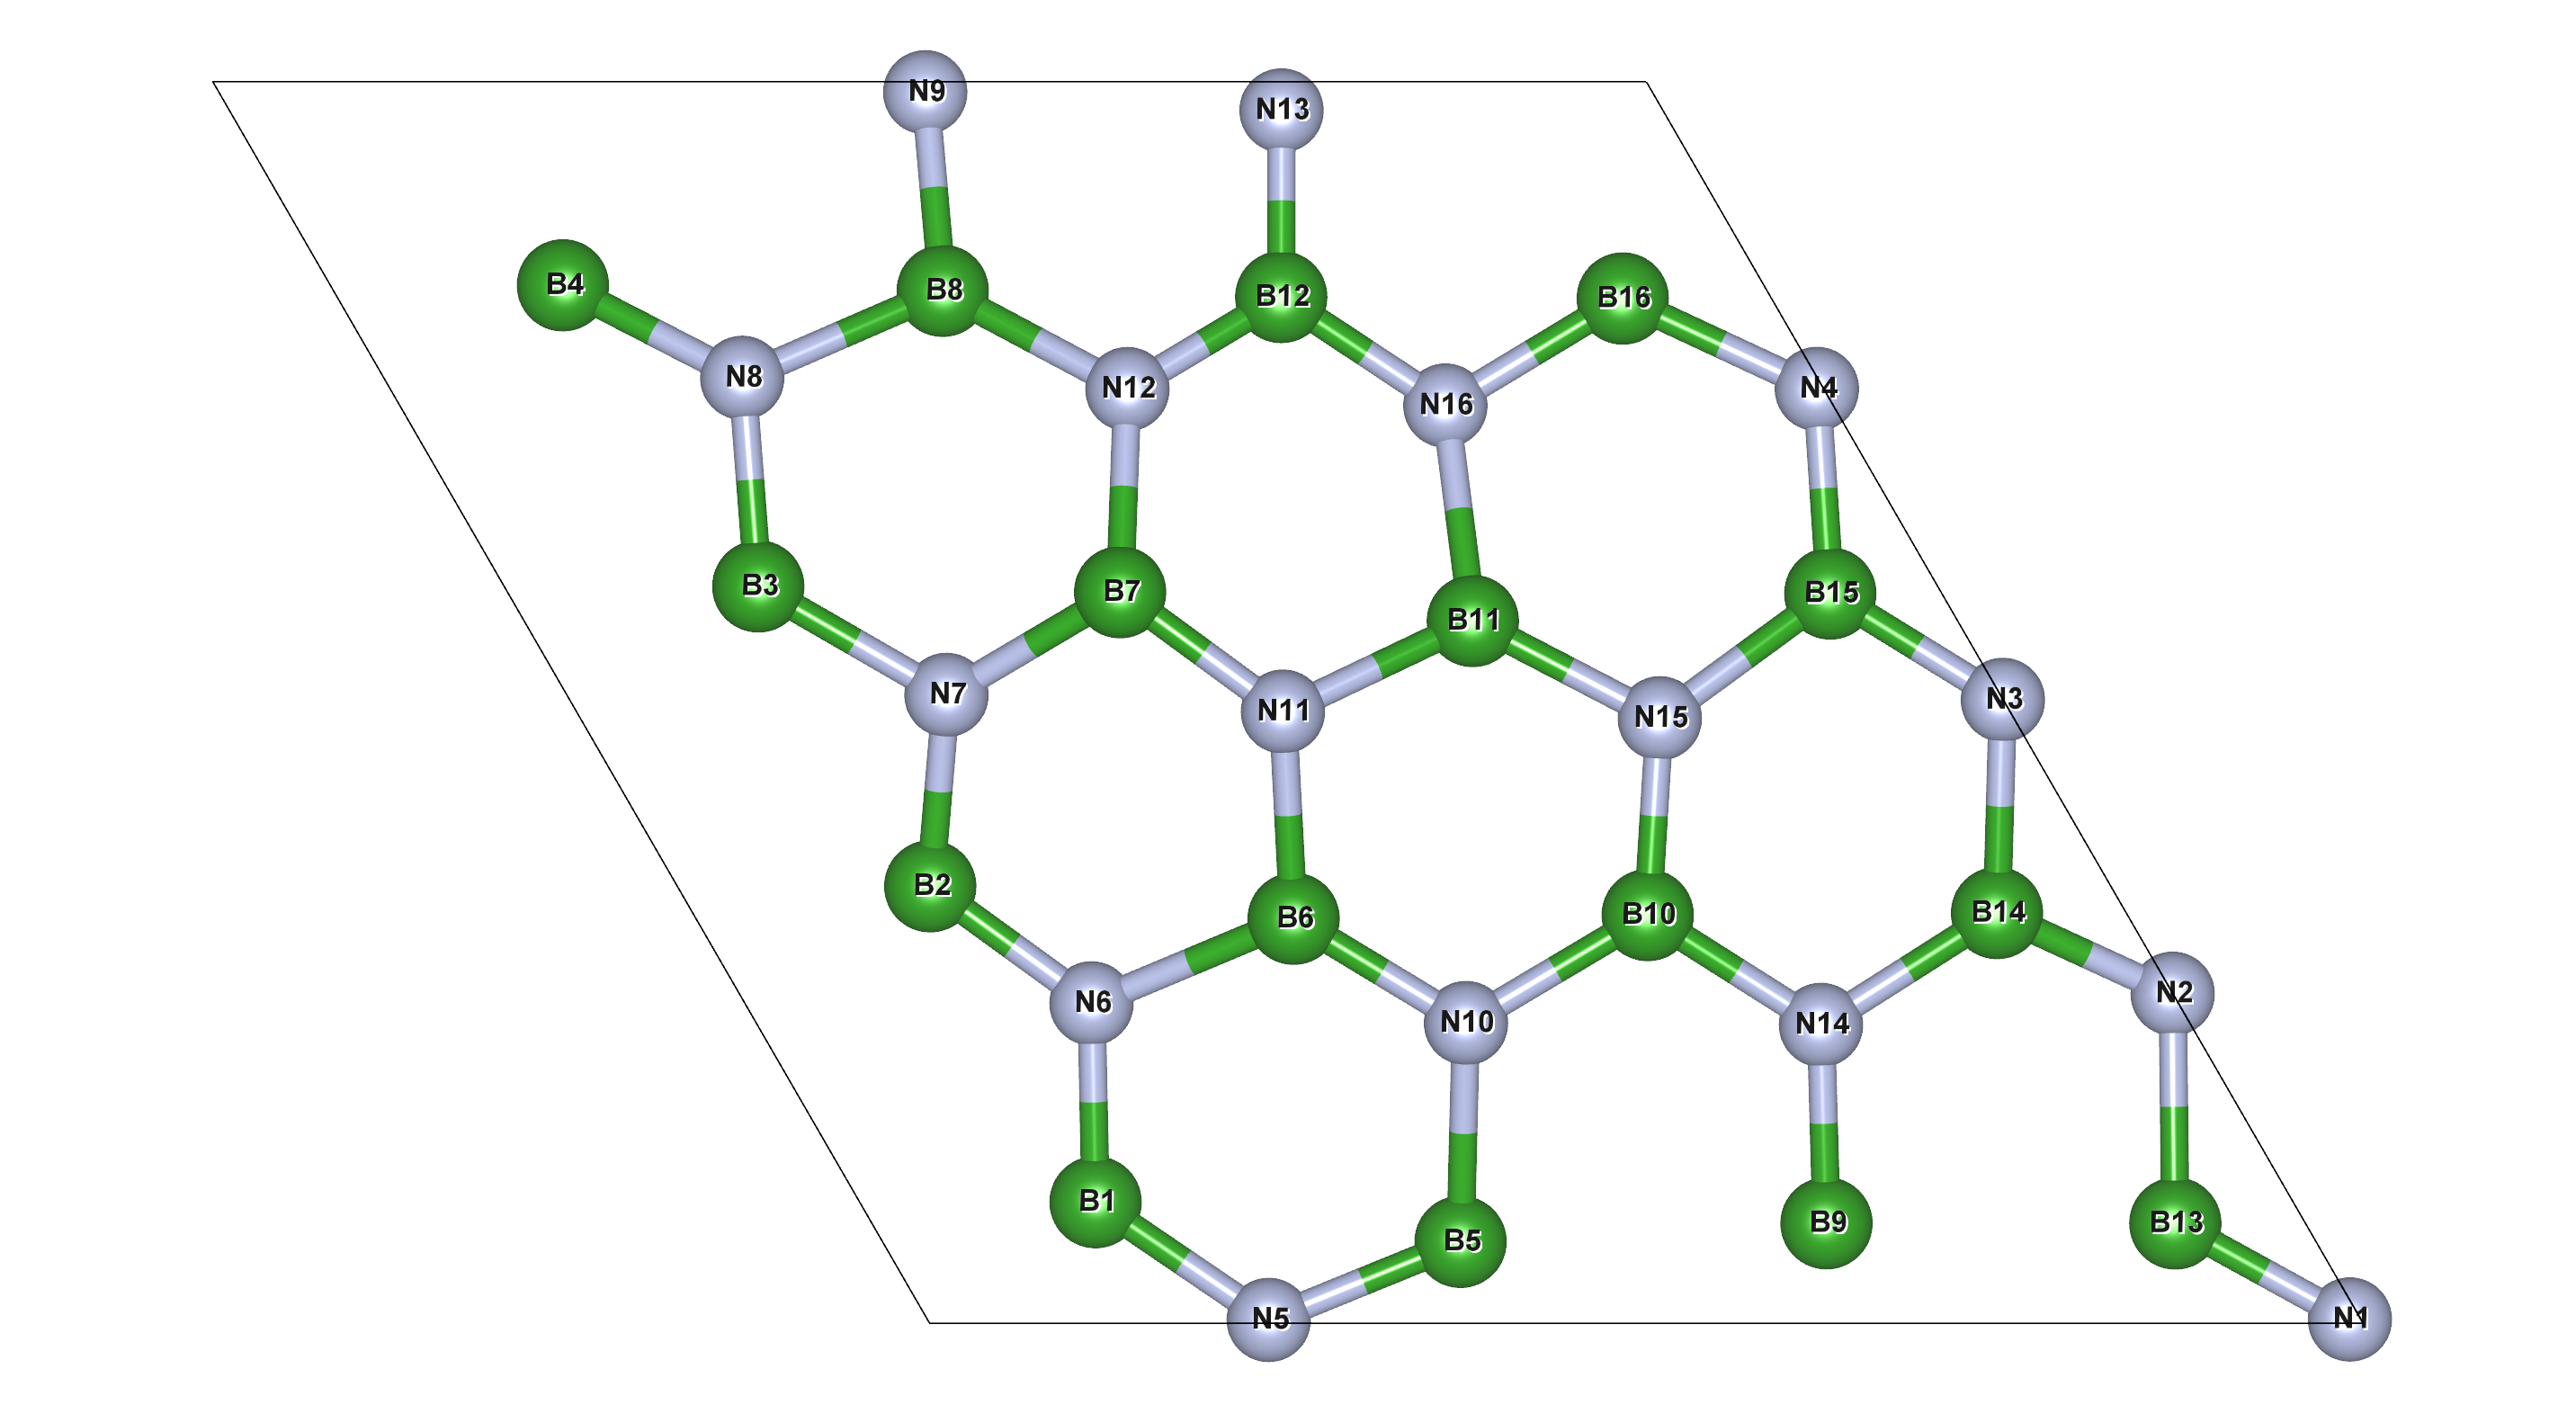
\includegraphics[width=0.49\linewidth]{gambar_hasil/hBN_pure_1225K.png}\hfill
    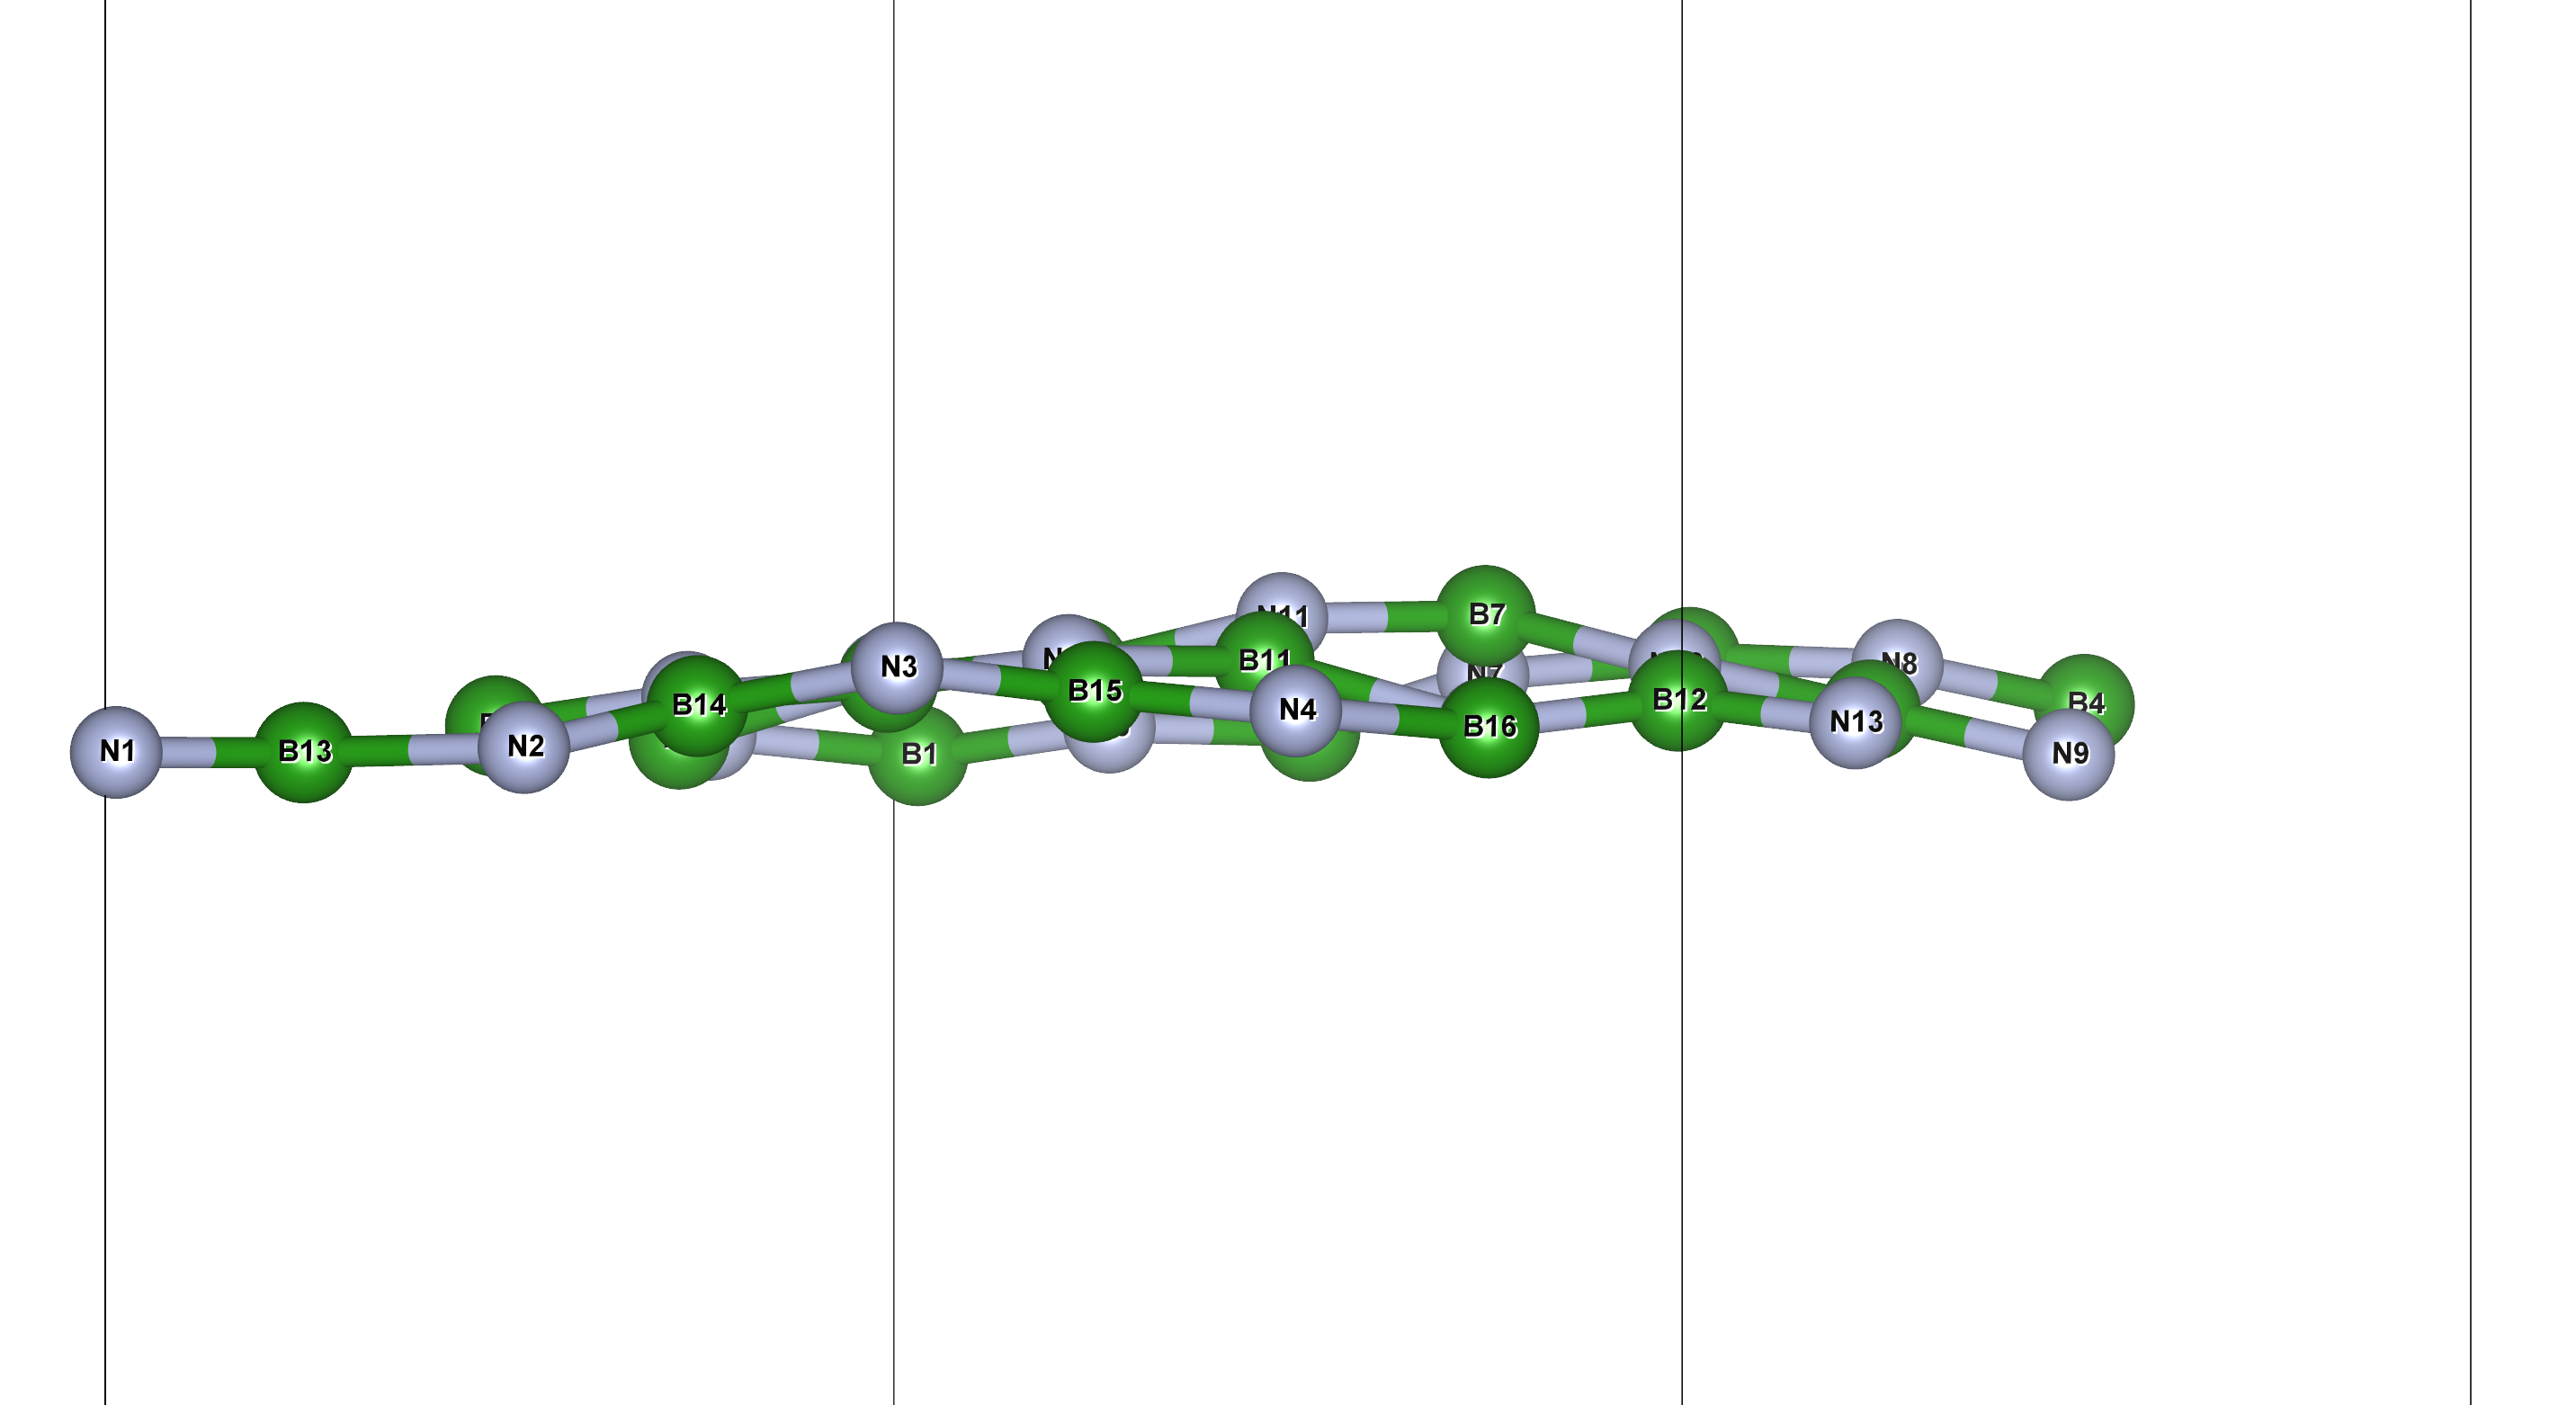
\includegraphics[width=0.49\linewidth]{gambar_hasil/hBN_pure_side_1225K.png}
    \caption{Murni, 1225 K}
    \label{subfig:md_pure_1225k}
  \end{subfigure}
\end{figure}

% --- Bagian 2: Cacat N_B (lanjutan) ---
\begin{figure}[htbp]\ContinuedFloat
  \centering
  \begin{subfigure}{\textwidth}
    \centering
    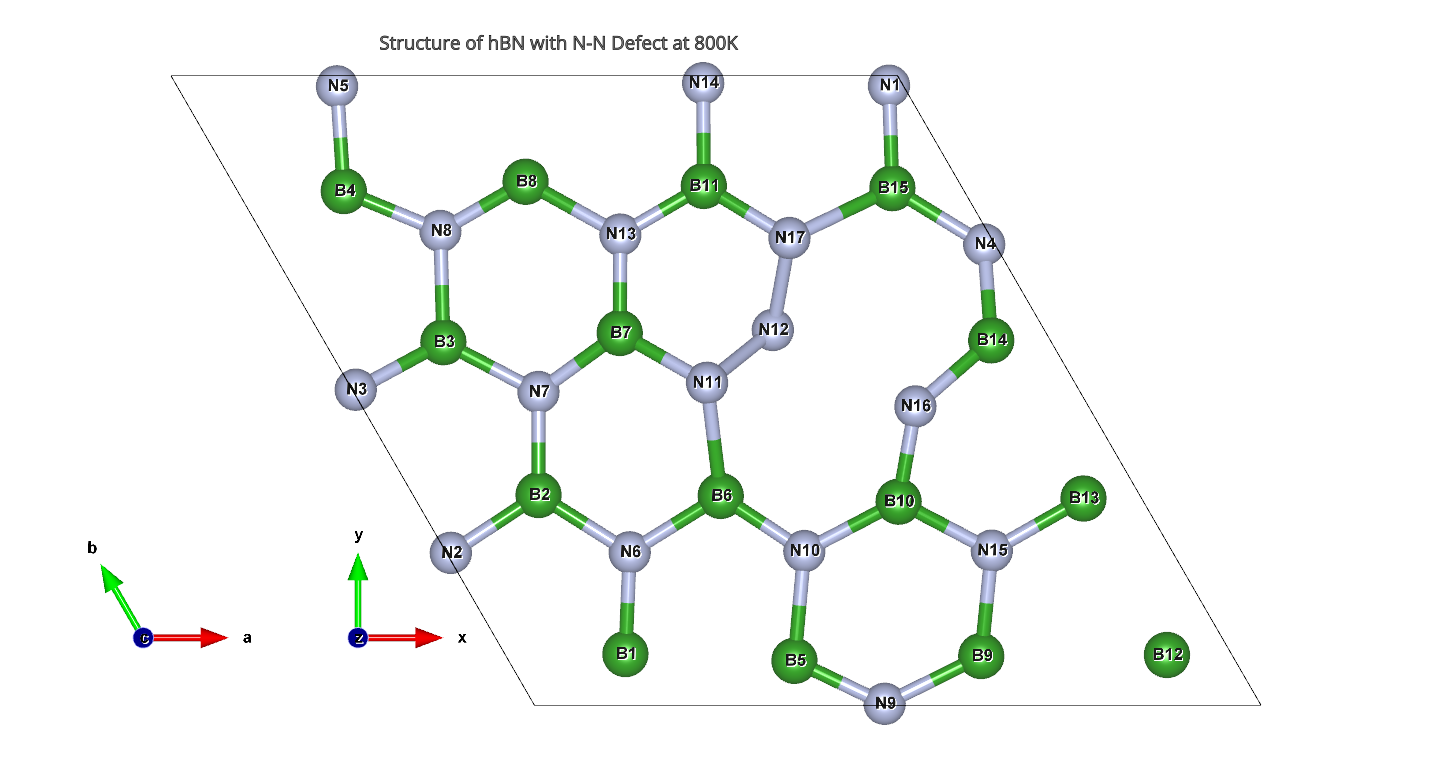
\includegraphics[width=0.49\linewidth]{gambar_hasil/hBN_NN_800K.png}\hfill
    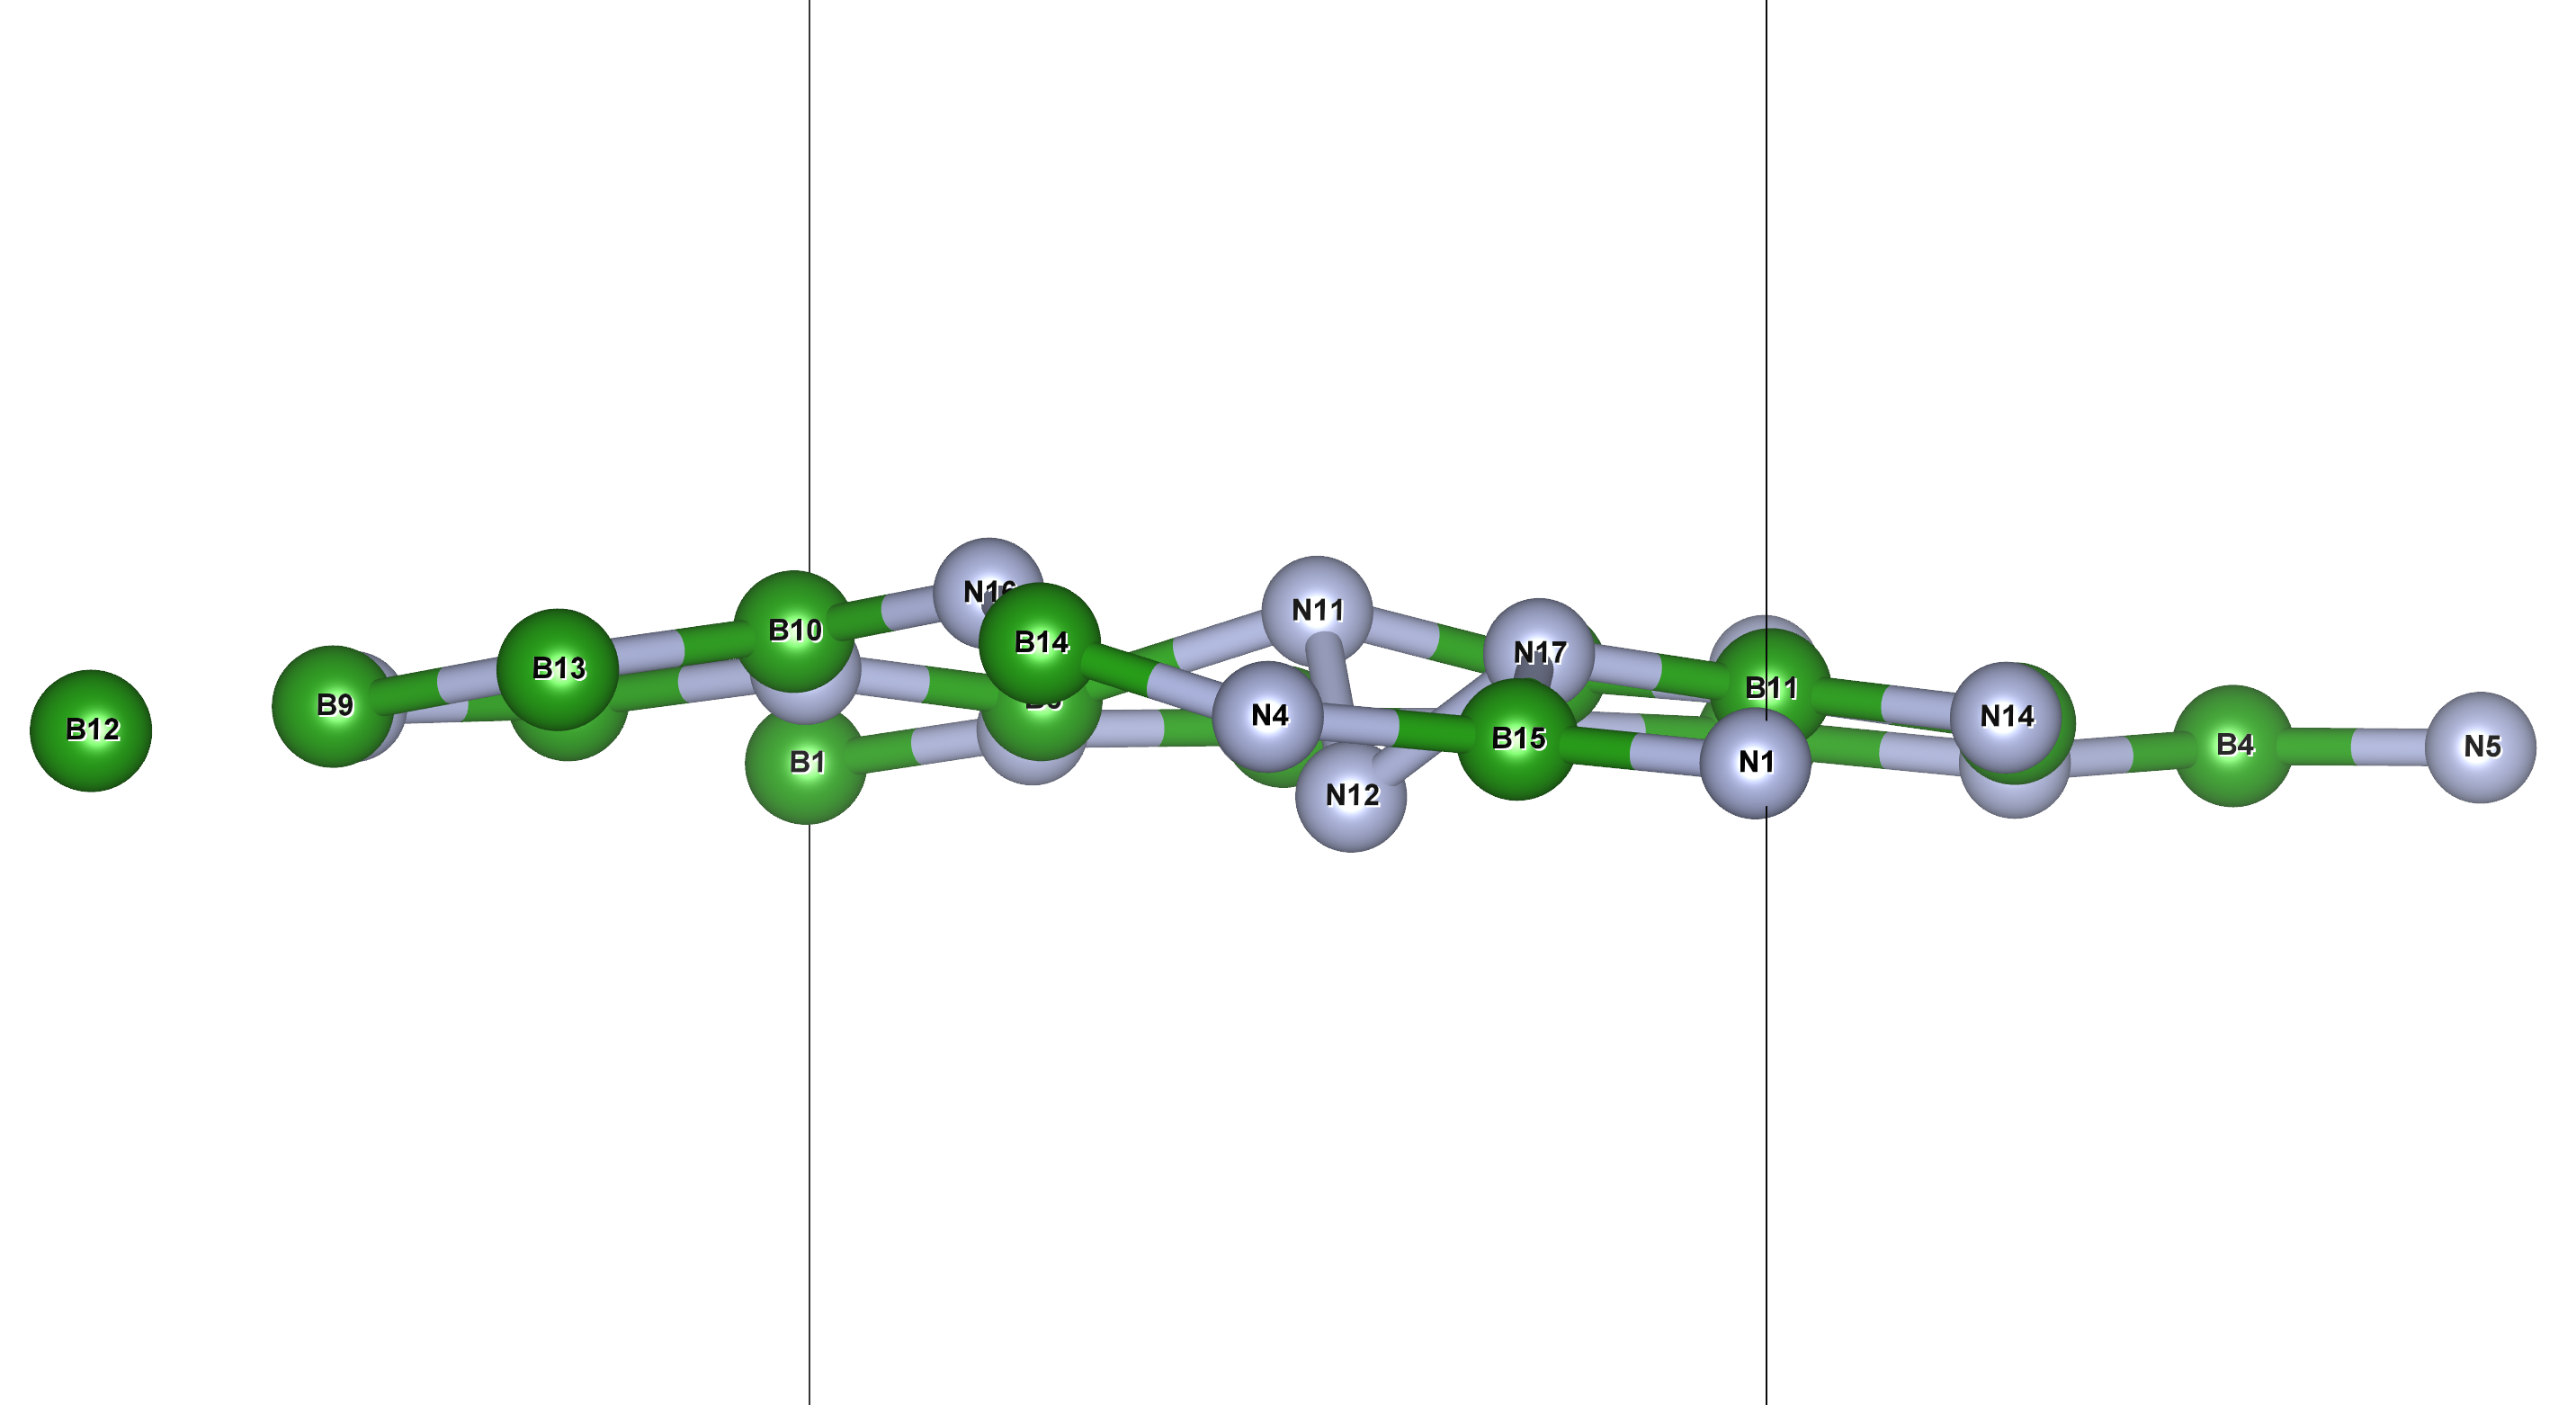
\includegraphics[width=0.49\linewidth]{gambar_hasil/hBN_NN_side_800K.png}
    \caption{Cacat N\textsubscript{B}, 800 K}
    \label{subfig:md_nn_800k}
  \end{subfigure}
  \vspace{1em}
  \begin{subfigure}{\textwidth}
    \centering
    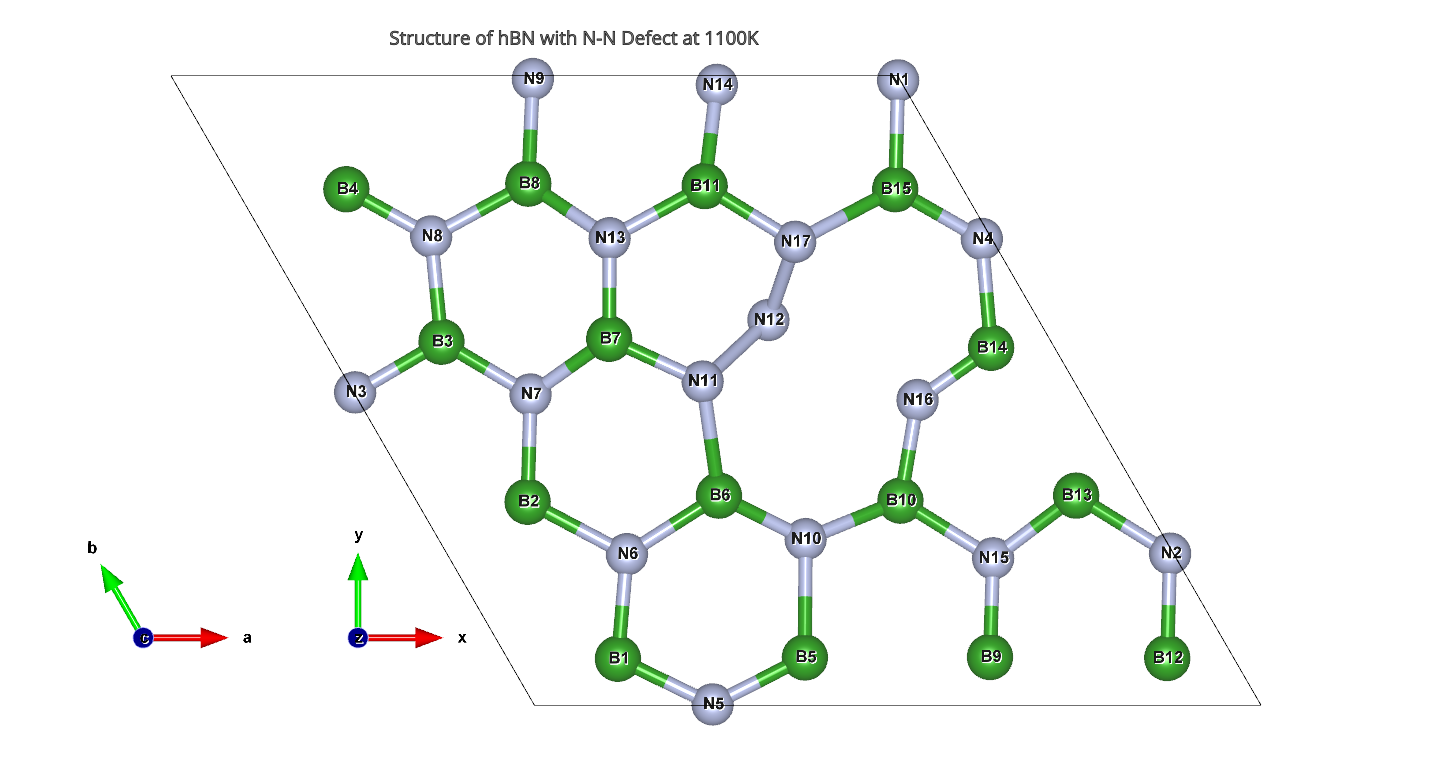
\includegraphics[width=0.49\linewidth]{gambar_hasil/hBN_NN_1100K.png}\hfill
    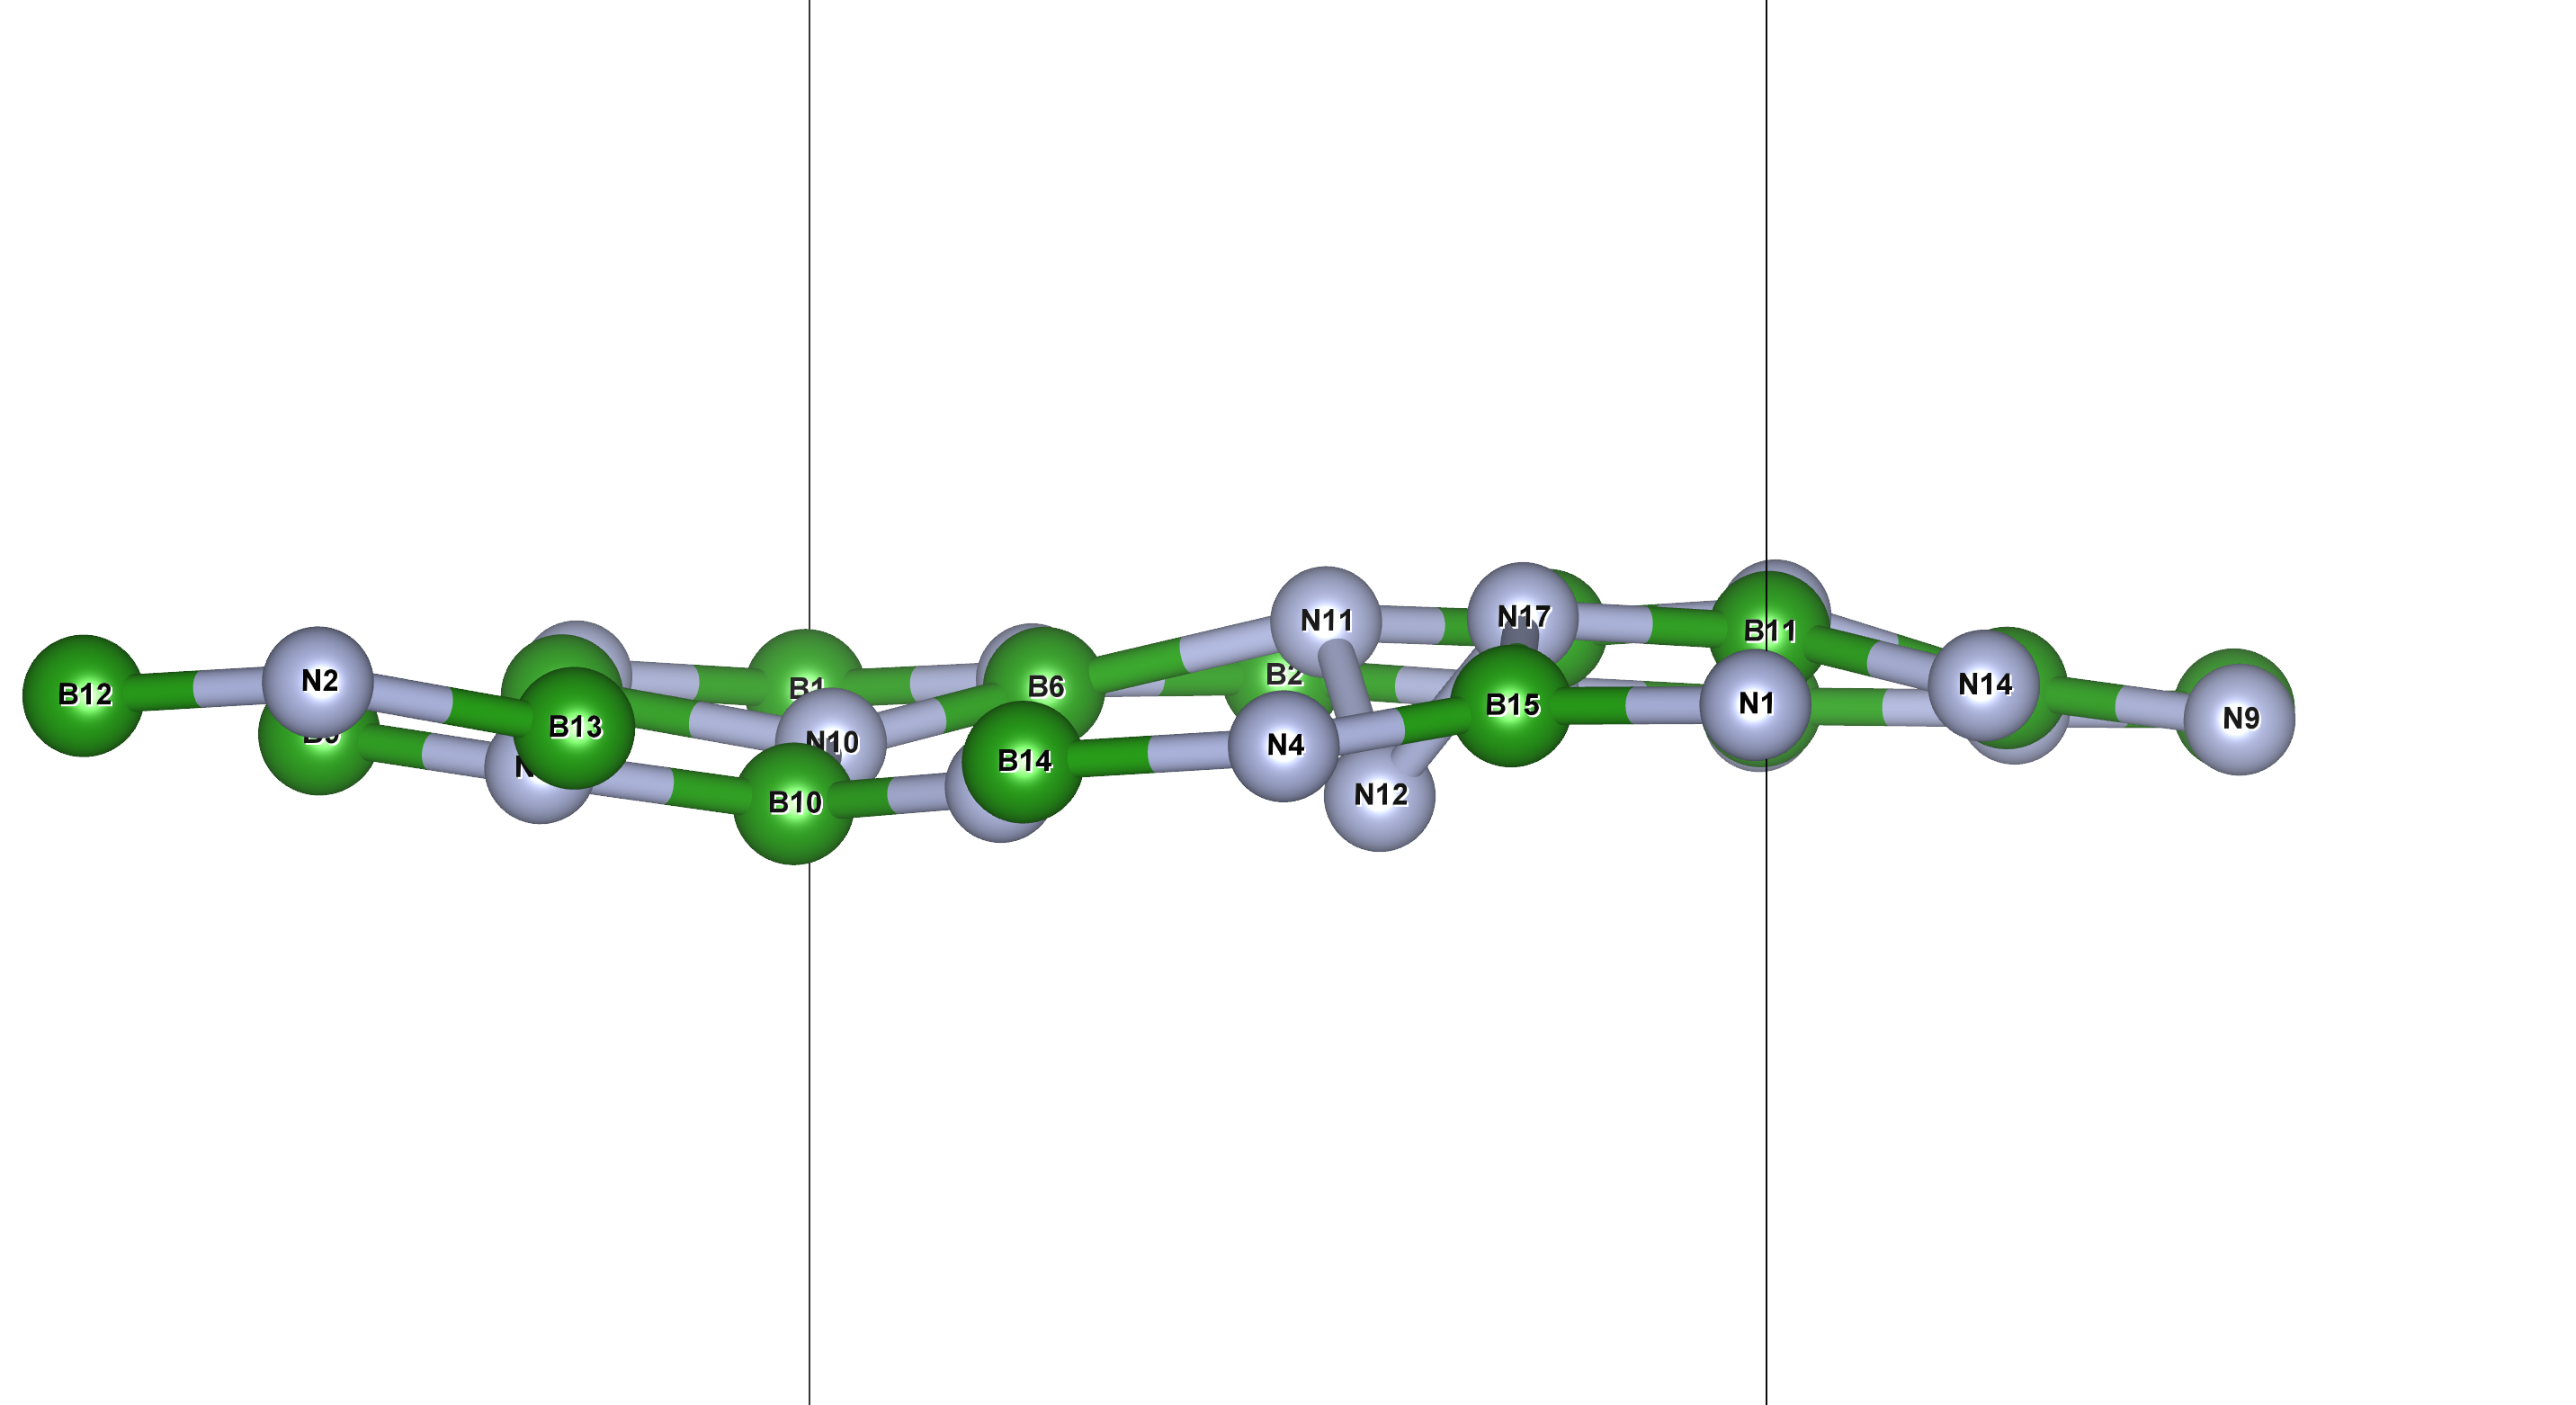
\includegraphics[width=0.49\linewidth]{gambar_hasil/hBN_NN_side_1100K.png}
    \caption{Cacat N\textsubscript{B}, 1100 K}
    \label{subfig:md_nn_1100k}
  \end{subfigure}
  \vspace{1em}
  \begin{subfigure}{\textwidth}
    \centering
    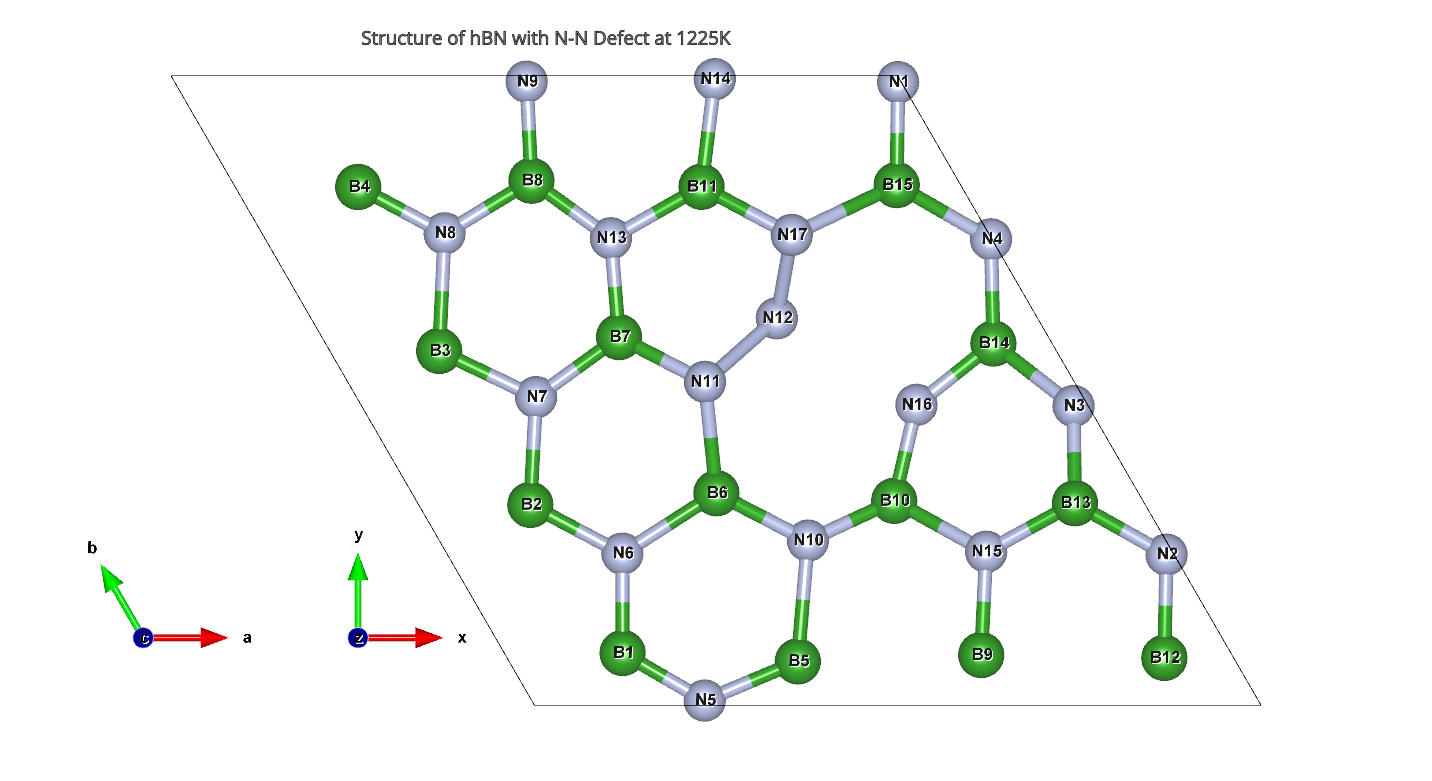
\includegraphics[width=0.49\linewidth]{gambar_hasil/hBN_NN_1225K.png}\hfill
    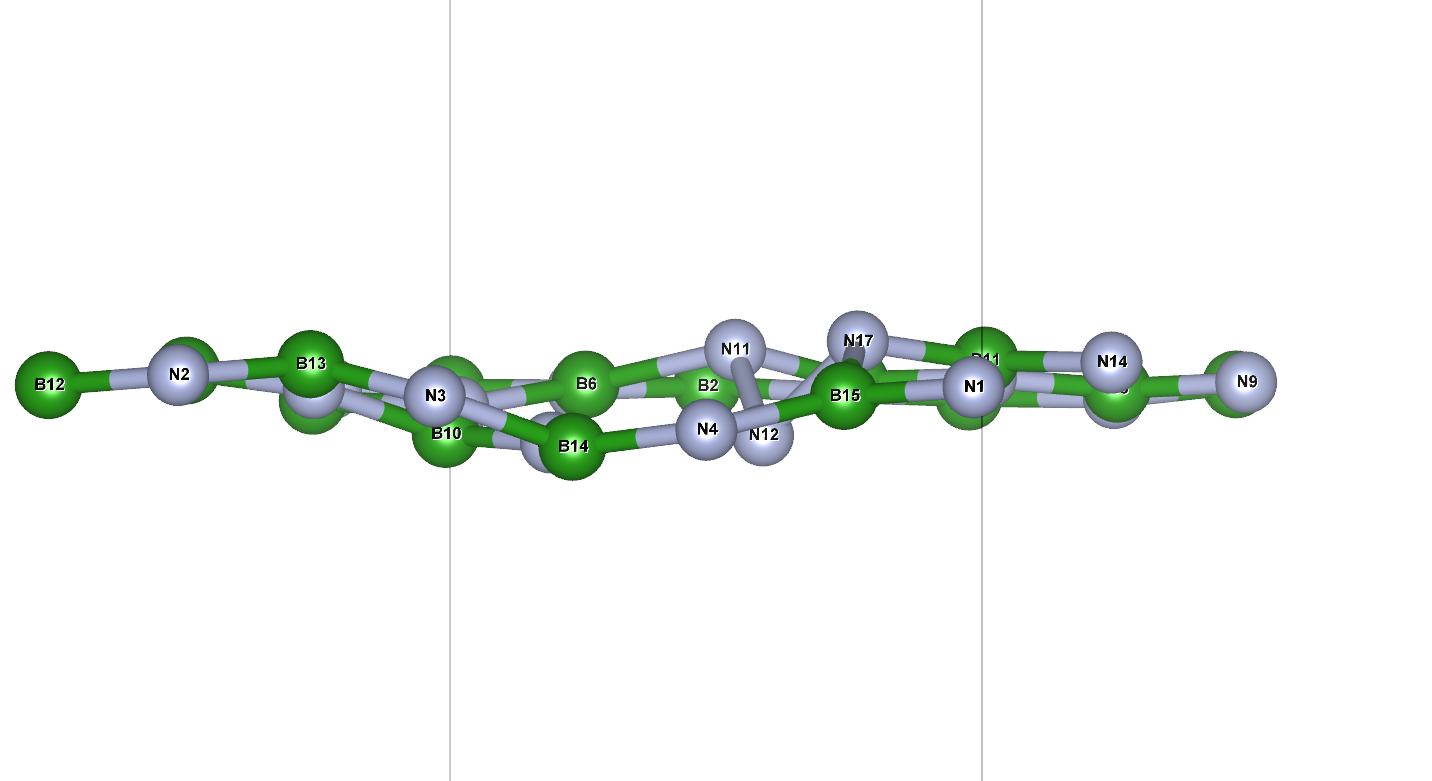
\includegraphics[width=0.49\linewidth]{gambar_hasil/hBN_NN_side_1225K.png}
    \caption{Cacat N\textsubscript{B}, 1225 K}
    \label{subfig:md_nn_1225k}
  \end{subfigure}
\end{figure}

% --- Bagian 3: Cacat B_N (lanjutan) ---
\begin{figure}[htbp]\ContinuedFloat
  \centering
  \begin{subfigure}{\textwidth}
    \centering
    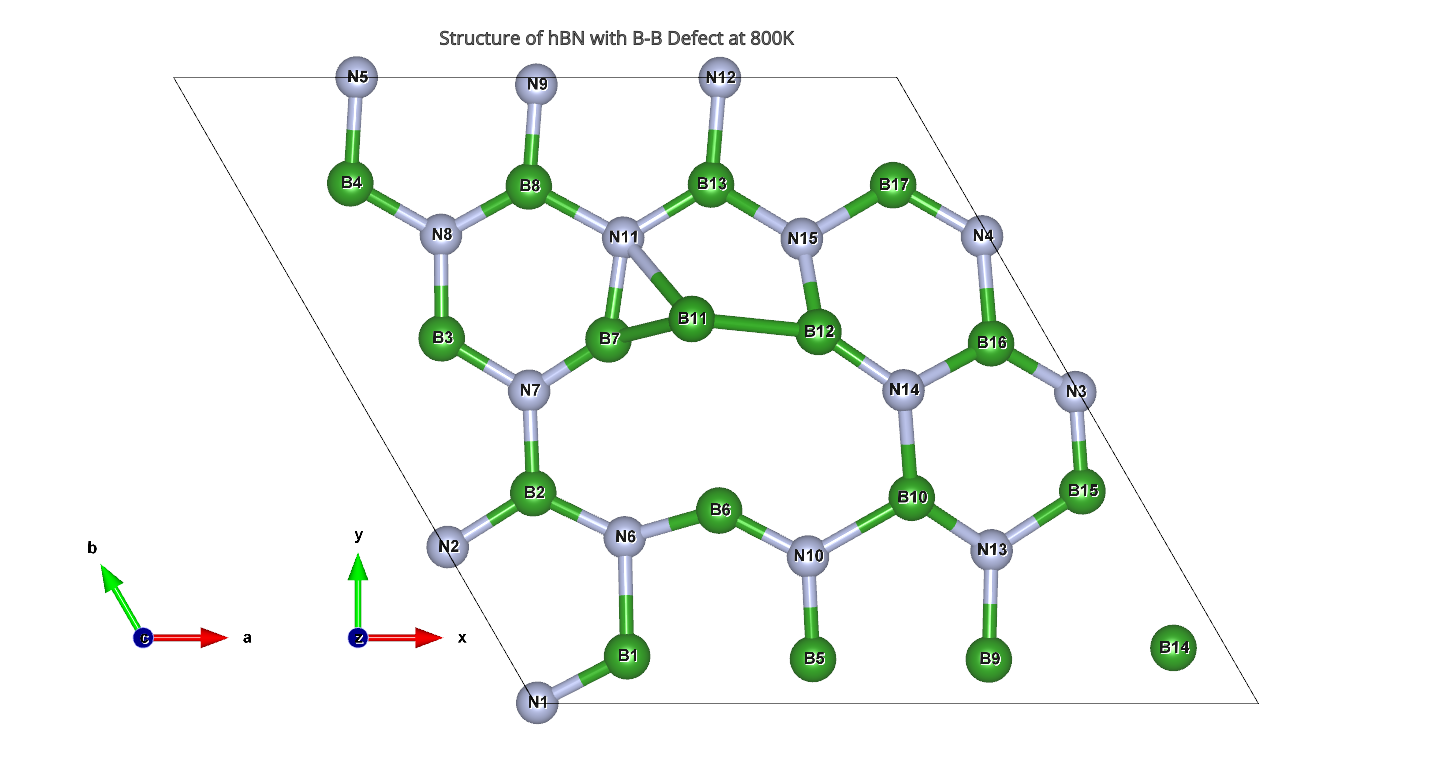
\includegraphics[width=0.49\linewidth]{gambar_hasil/hBN_BB_800K.png}\hfill
    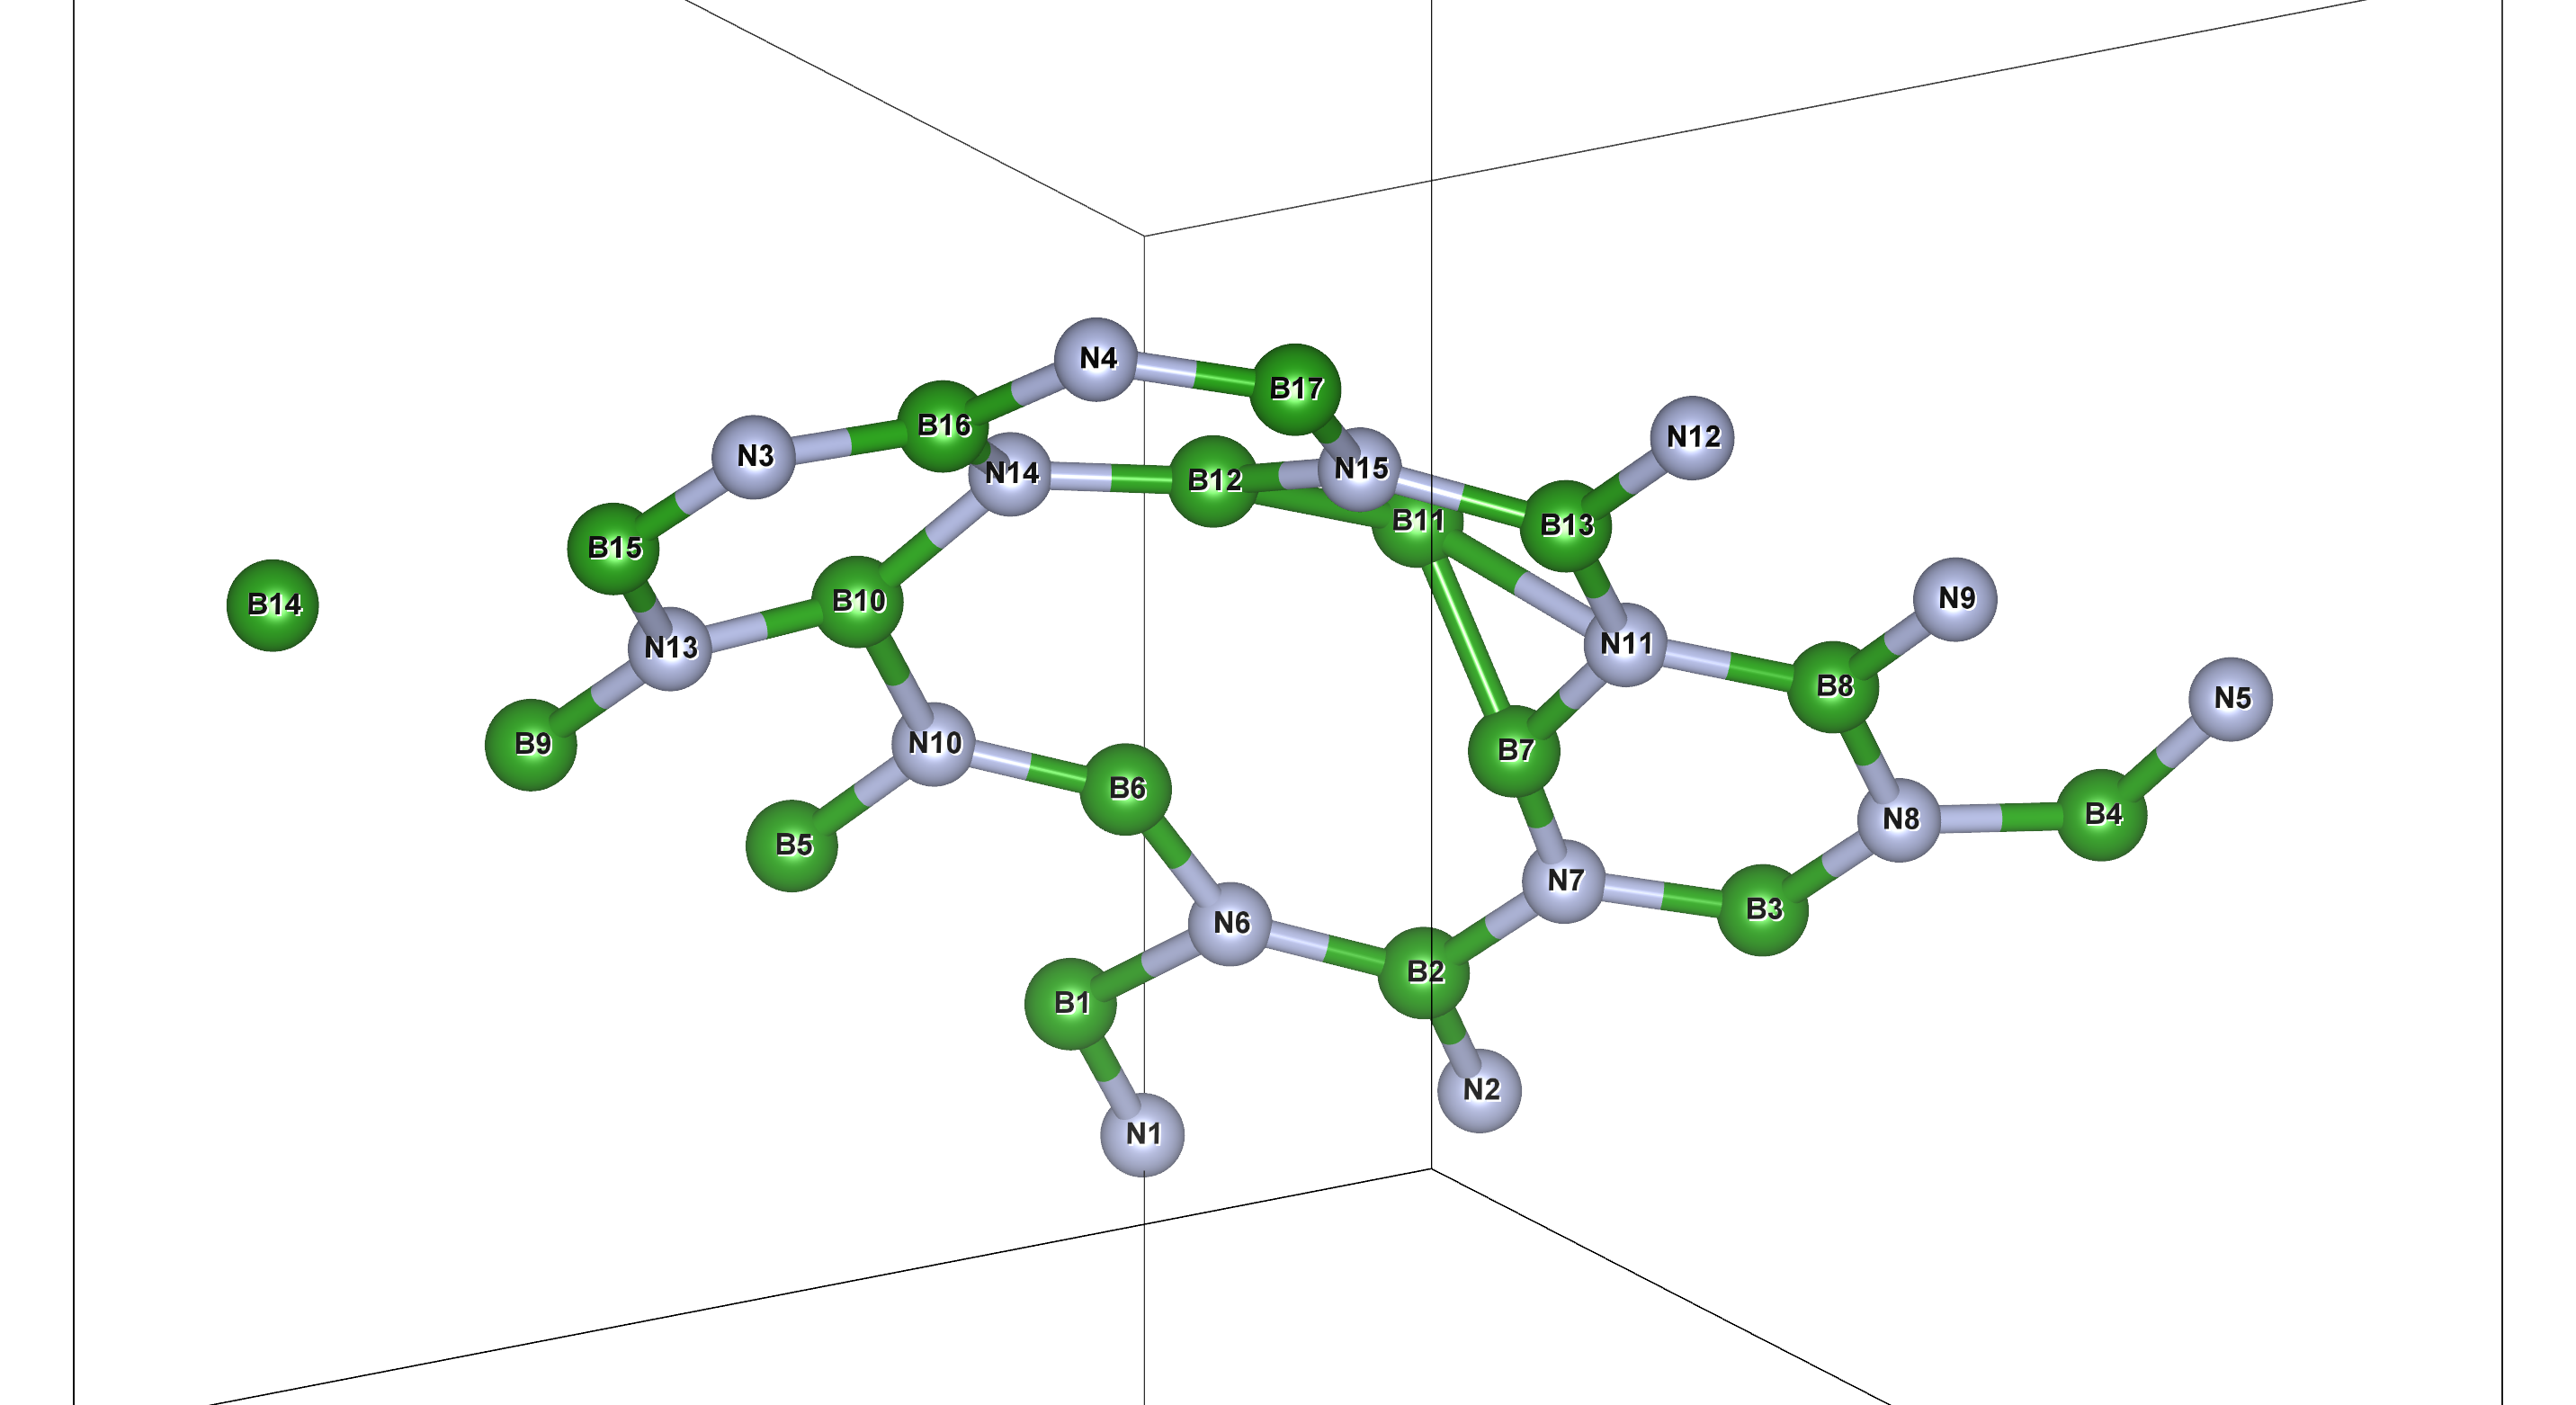
\includegraphics[width=0.49\linewidth]{gambar_hasil/hBN_BB_side_800K.png}
    \caption{Cacat B\textsubscript{N}, 800 K}
    \label{subfig:md_bb_800k}
  \end{subfigure}
  \vspace{1em}
  \begin{subfigure}{\textwidth}
    \centering
    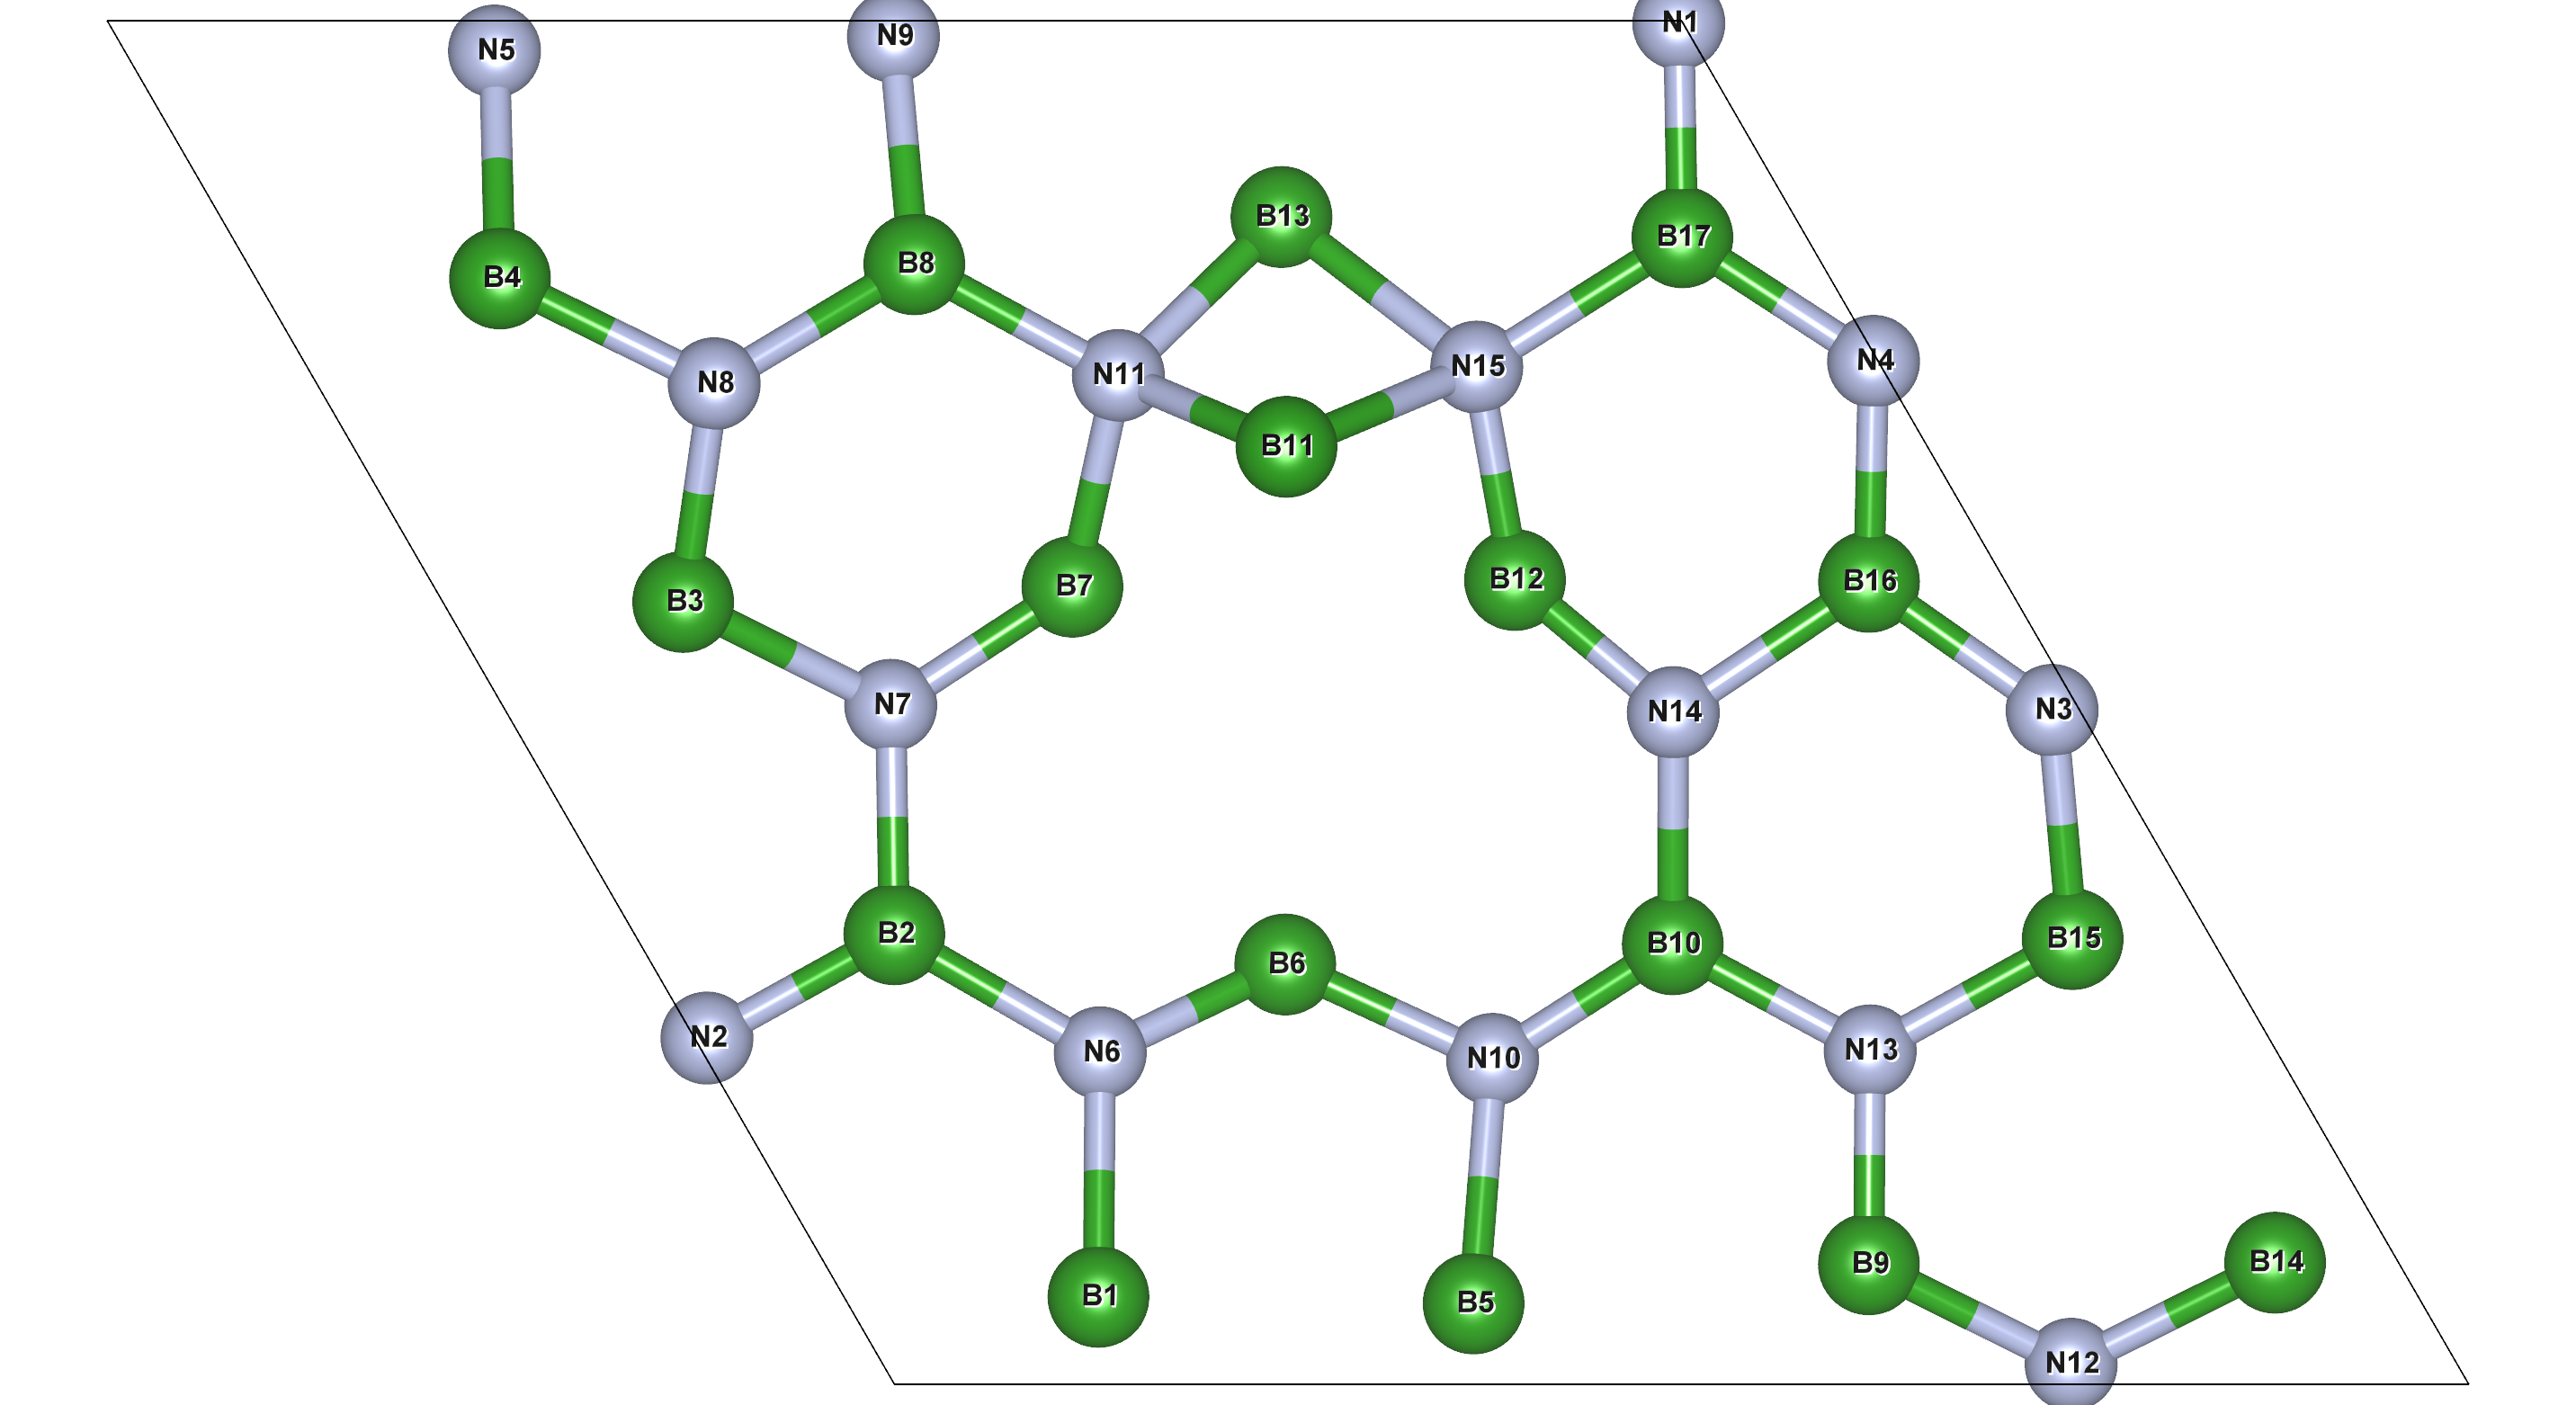
\includegraphics[width=0.49\linewidth]{gambar_hasil/hBN_BB_1100K.png}\hfill
    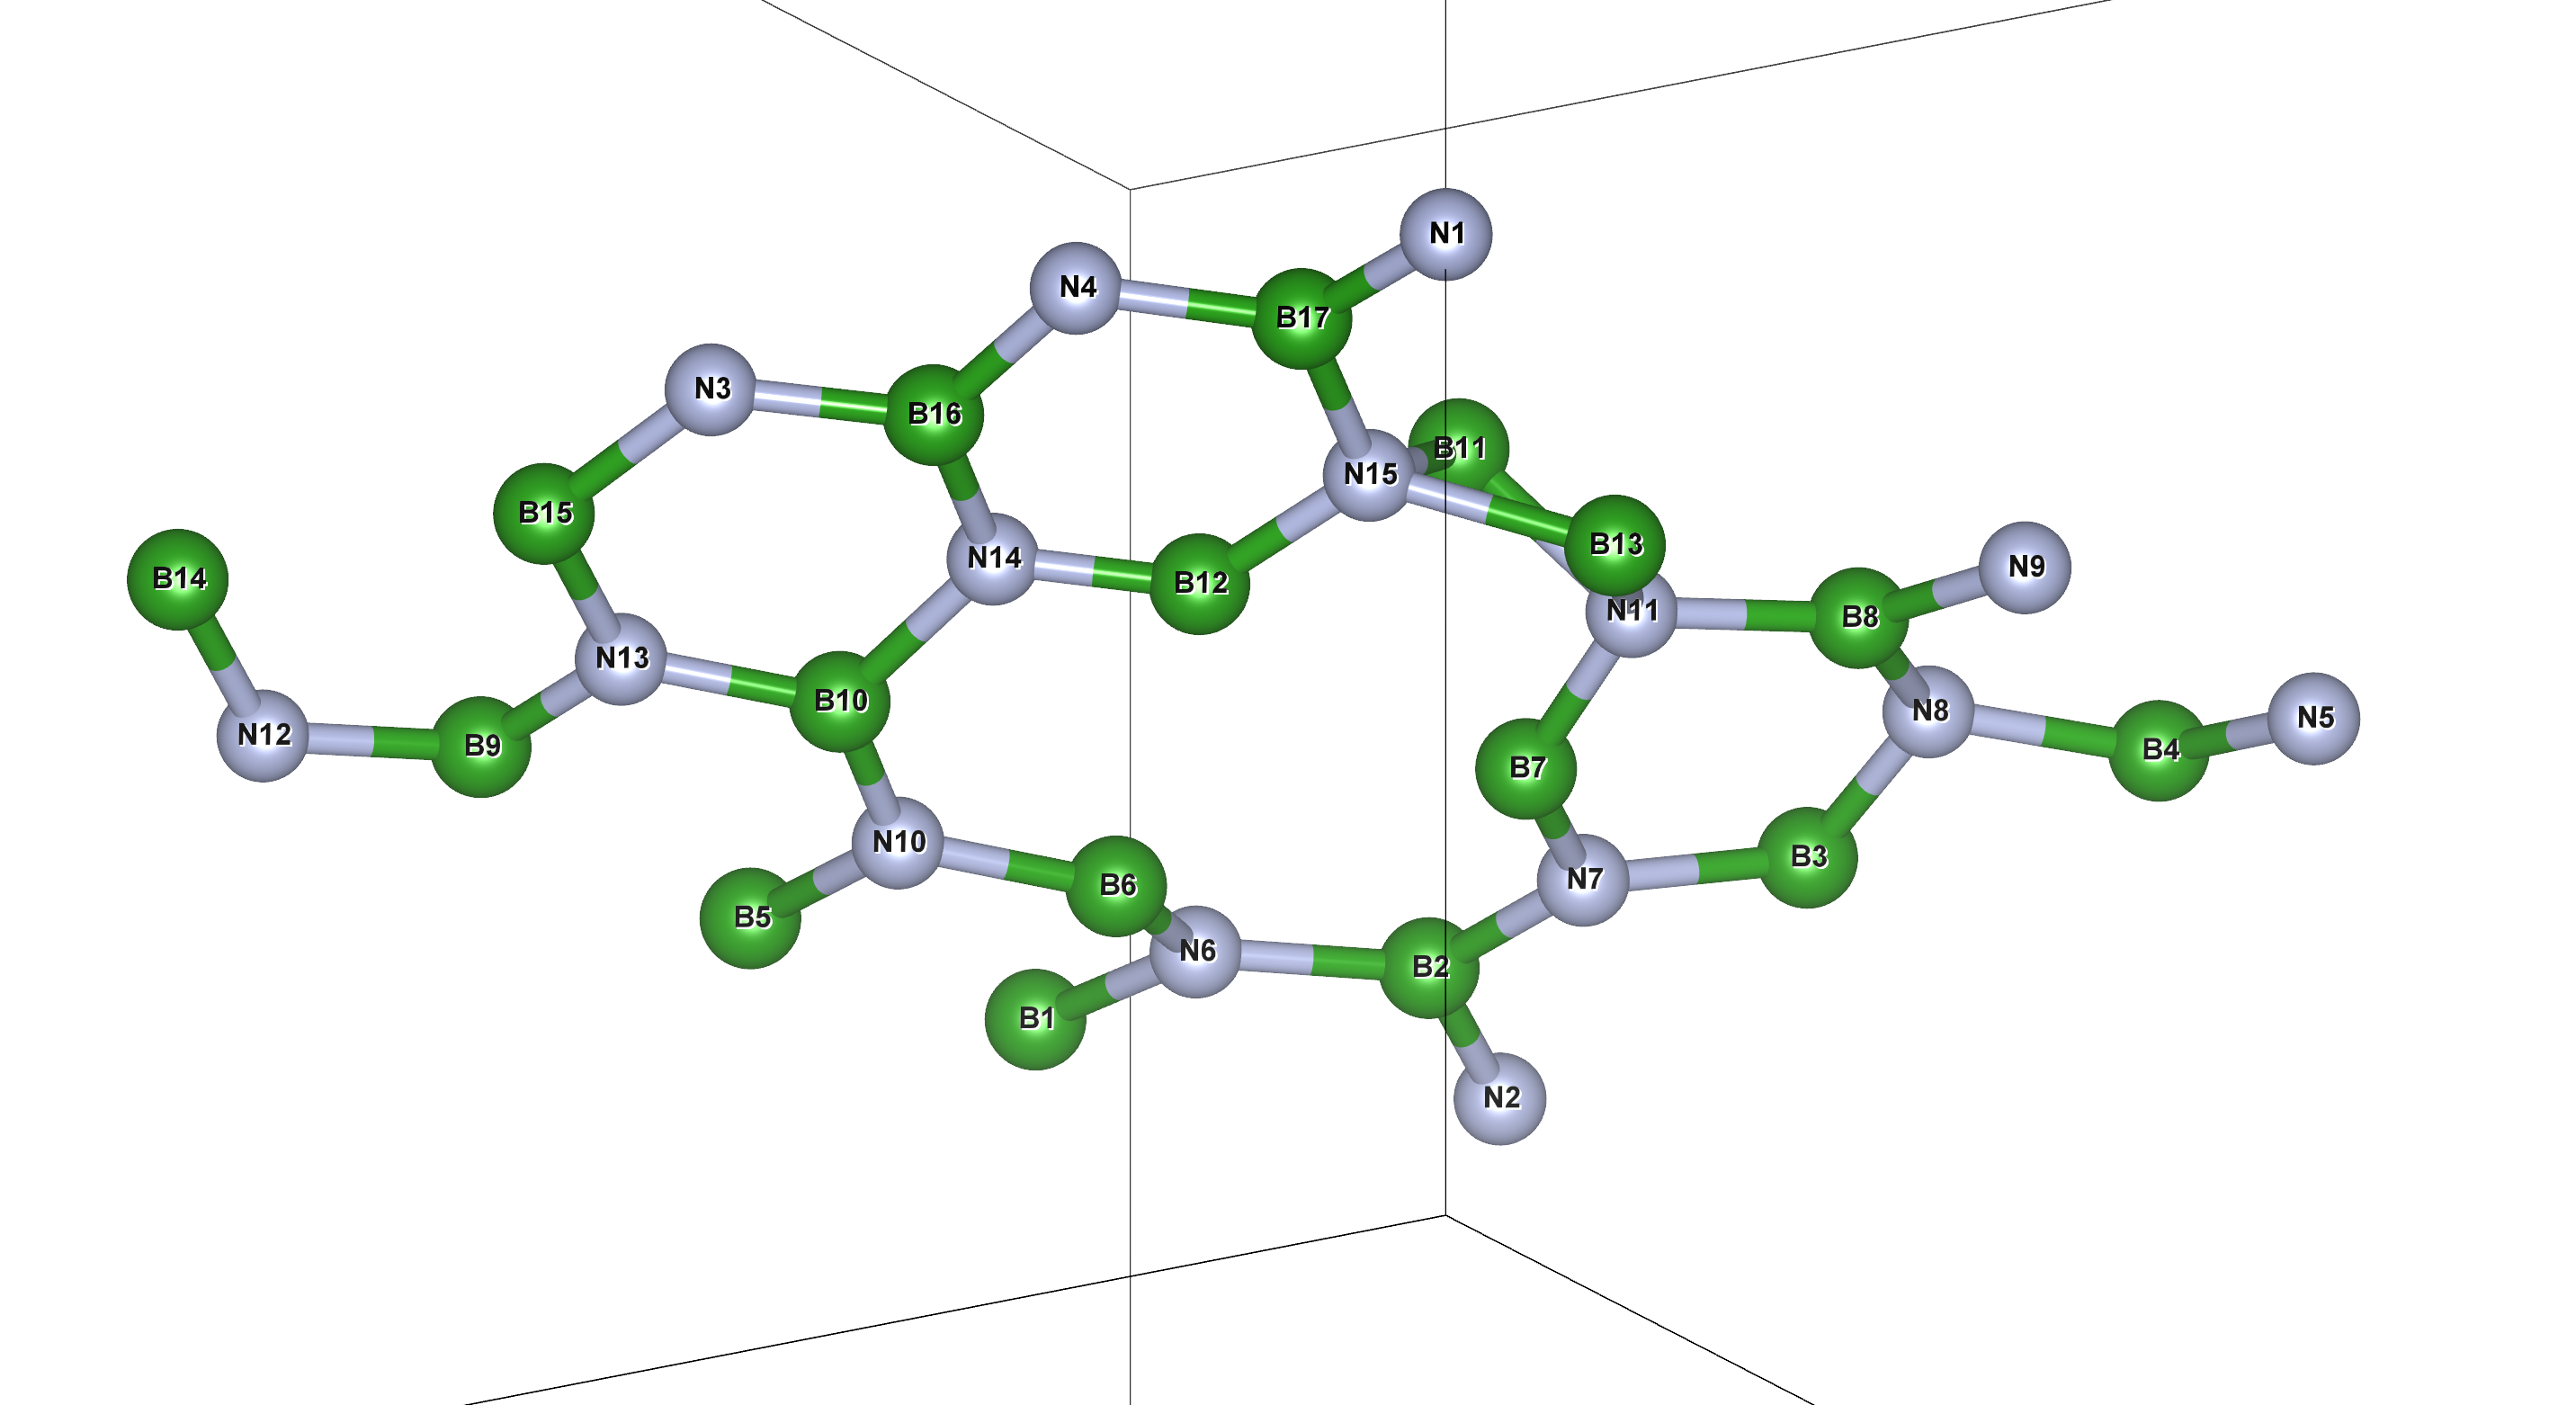
\includegraphics[width=0.49\linewidth]{gambar_hasil/hBN_BB_side_1100K.png}
    \caption{Cacat B\textsubscript{N}, 1100 K}
    \label{subfig:md_bb_1100k}
  \end{subfigure}
  \vspace{1em}
  \begin{subfigure}{\textwidth}
    \centering
    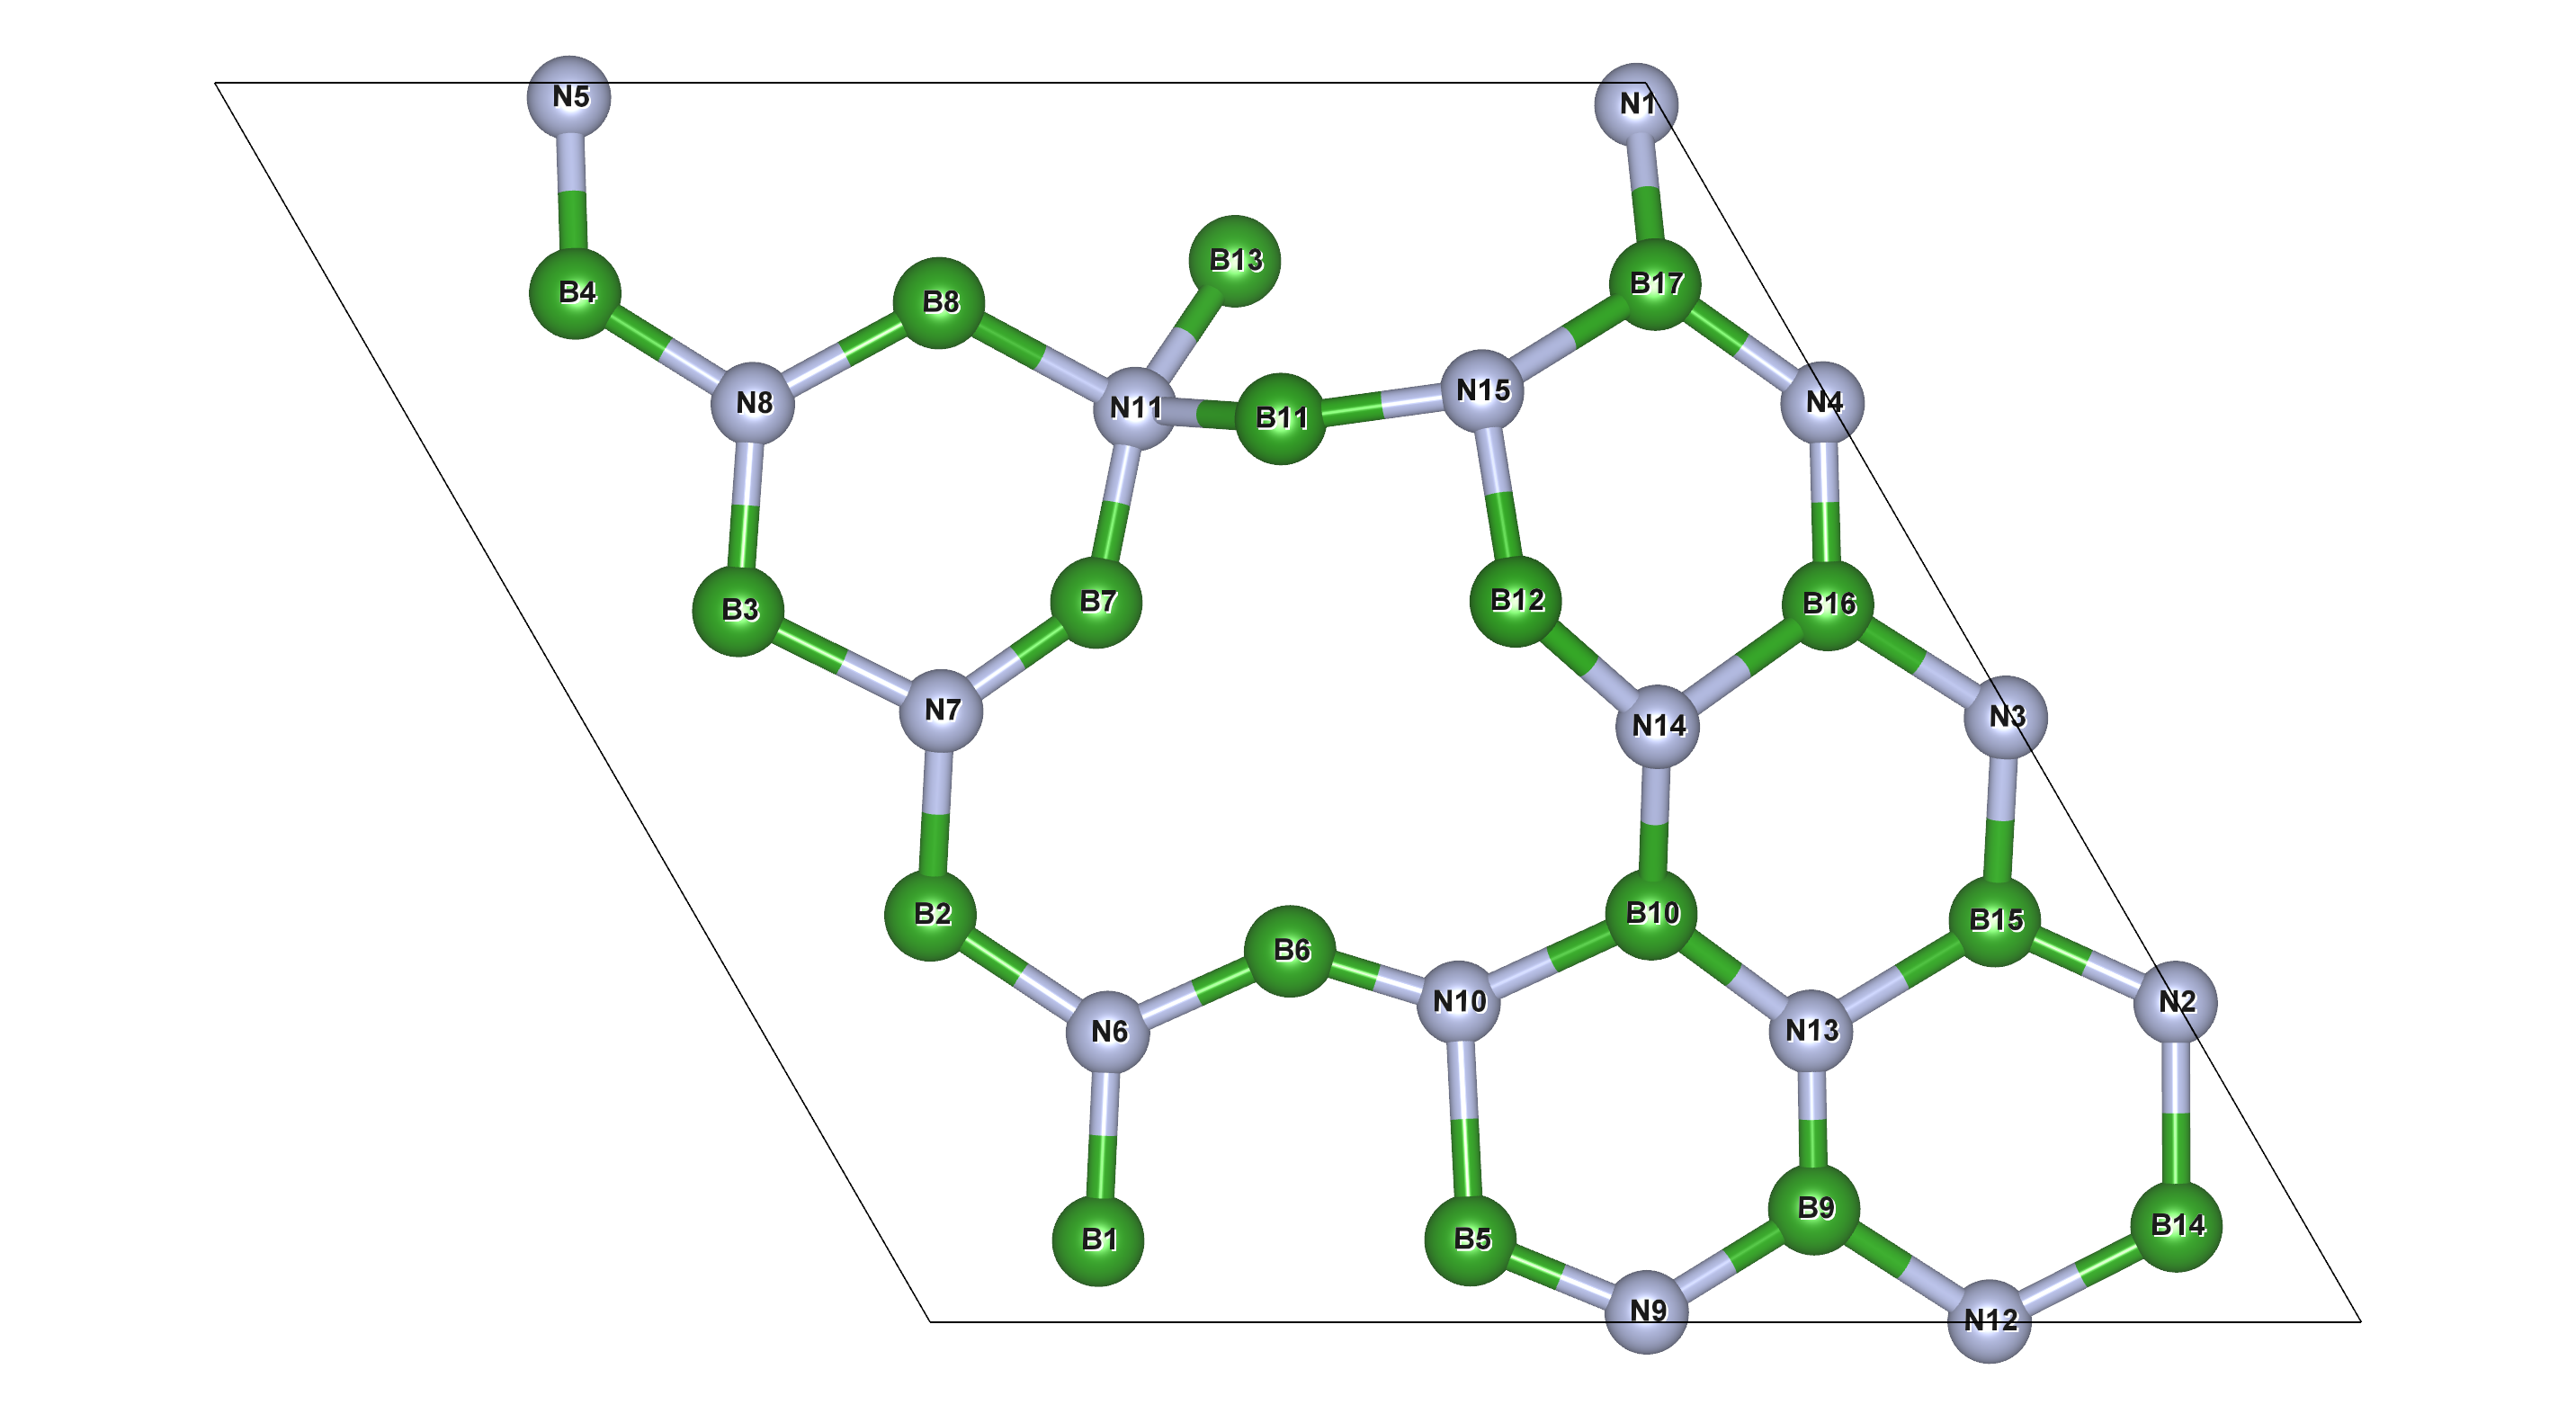
\includegraphics[width=0.49\linewidth]{gambar_hasil/hBN_BB_1225K.png}\hfill
    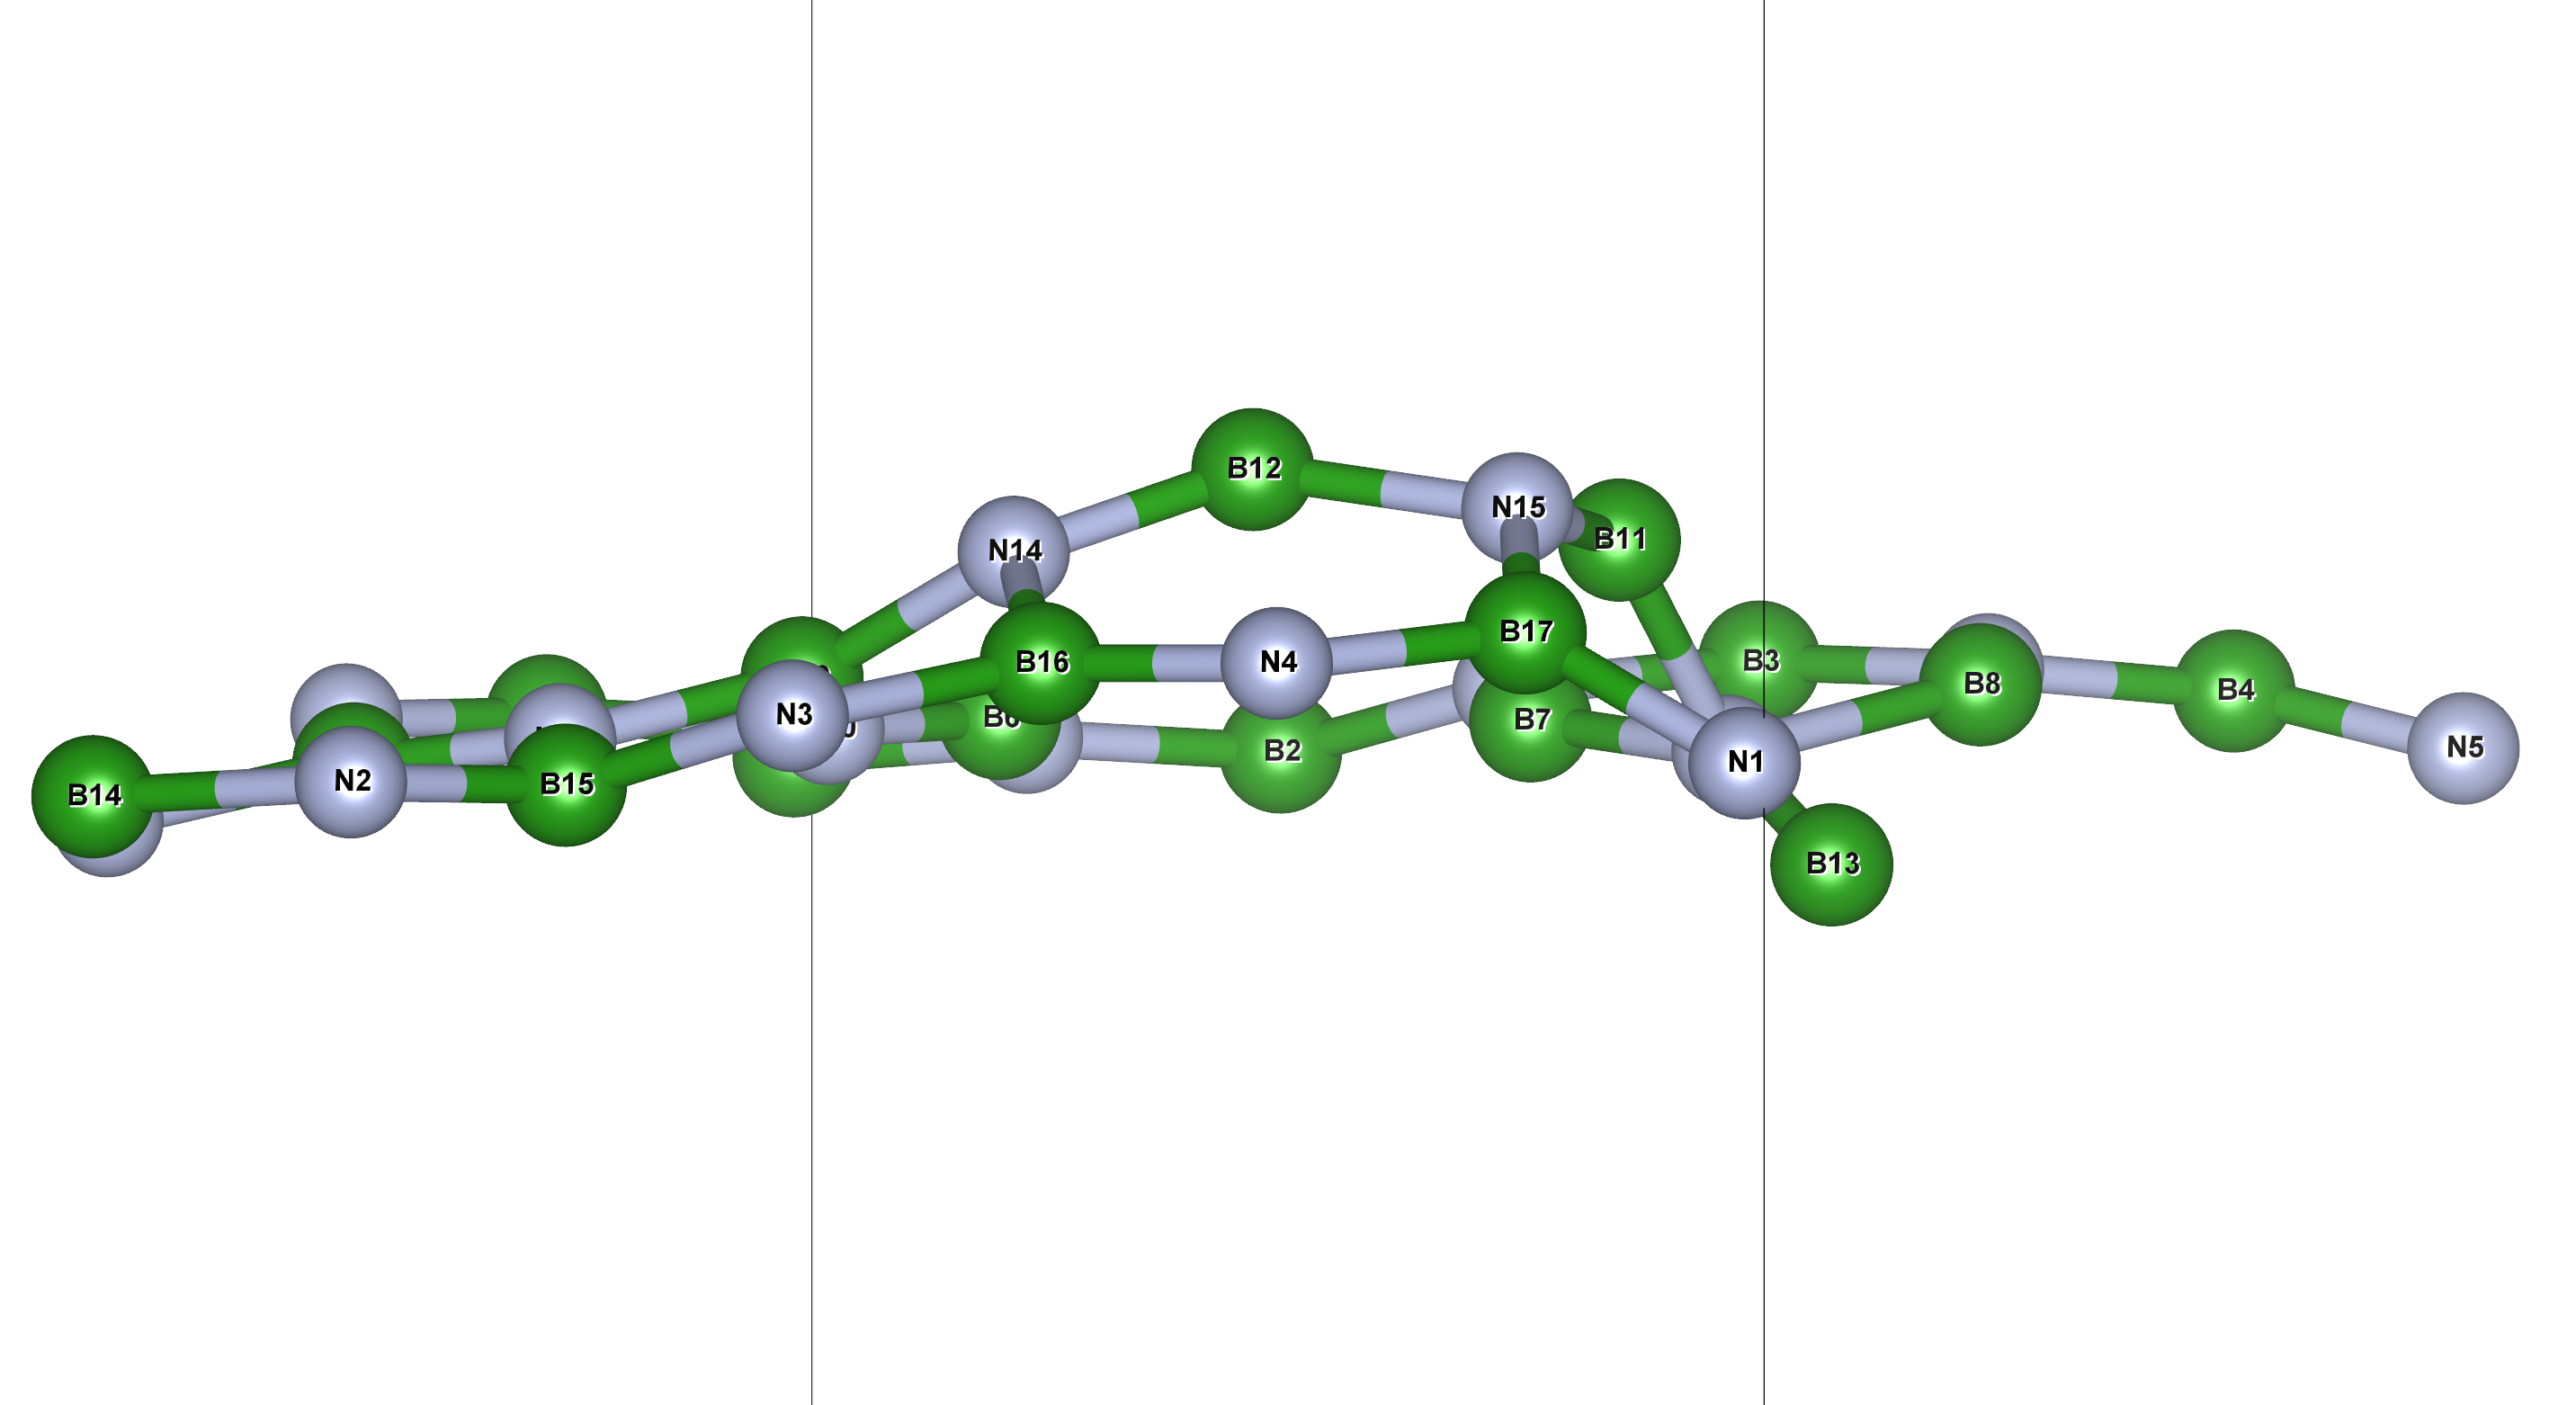
\includegraphics[width=0.49\linewidth]{gambar_hasil/hBN_BB_side_1225K.png}
    \caption{Cacat B\textsubscript{N}, 1225 K}
    \label{subfig:md_bb_1225k}
  \end{subfigure}
    \caption{Visualisasi struktur atomik hasil pemanasan MD. Setiap baris menampilkan tampak atas dan samping untuk sistem dan temperatur yang spesifik.}
  \label{fig:md_structures_per_condition}
\end{figure}

Seperti yang diilustrasikan secara skematis pada Gambar \ref{fig:md_structures_per_condition}, distorsi ini menjadi lebih jelas pada sistem yang mengandung cacat.
Cacat titik bertindak sebagai pusat tegangan (\emph{strain}) lokal, mengganggu keteraturan kisi di sekitarnya dan seringkali memperkuat amplitudo riak termal.
Analisis kuantitatif dari gangguan struktural ini dapat diperoleh melalui fungsi distribusi radial dan pergeseran kuadrat rata-rata.

\subsection{Analisis Tatanan Struktural dan Mobilitas Atomik: RDF dan MSD}
\label{subsec:md_rdf_msd}
Fungsi Distribusi Radial, $g(r)$, memberikan informasi statistik tentang probabilitas menemukan atom pada jarak $r$ dari atom referensi.
Ini adalah alat yang ampuh untuk mengukur tatanan struktural. Pergeseran Kuadrat Rata-rata (MSD) mengukur rata-rata jarak kuadrat yang ditempuh oleh atom dari posisi awalnya seiring waktu.
Ini memberikan wawasan tentang dinamika dan stabilitas struktural material.

%%%%%%%%%%%%%%%%%%%%%%%%%%%%%%%%%%%%%%%%%%%%%%%%%%%%%%%%%%%%%%%%%%%%%%
% PERBAIKAN GAMBAR 2: PLOT RDF DAN MSD (Tata Letak Vertikal, Ukuran Besar)
% Permintaan: Tumpukan vertikal, lebih besar, dan dapat pindah halaman.
% Solusi: Setiap plot ditempatkan dalam 'subfigure' dengan lebar 0.85\textwidth,
% membuatnya sangat jelas dan mudah dibaca. Tumpukan vertikal dari 9 plot ini
% akan menghasilkan 'figure' yang sangat tinggi, yang akan ditangani oleh
% mekanisme float LaTeX ([htbp!]) dengan memindahkannya ke halaman float [p].
%%%%%%%%%%%%%%%%%%%%%%%%%%%%%%%%%%%%%%%%%%%%%%%%%%%%%%%%%%%%%%%%%%%%%%
\begin{figure}[htbp]
  \centering
  \begin{subfigure}{0.9\textwidth}
    \centering
    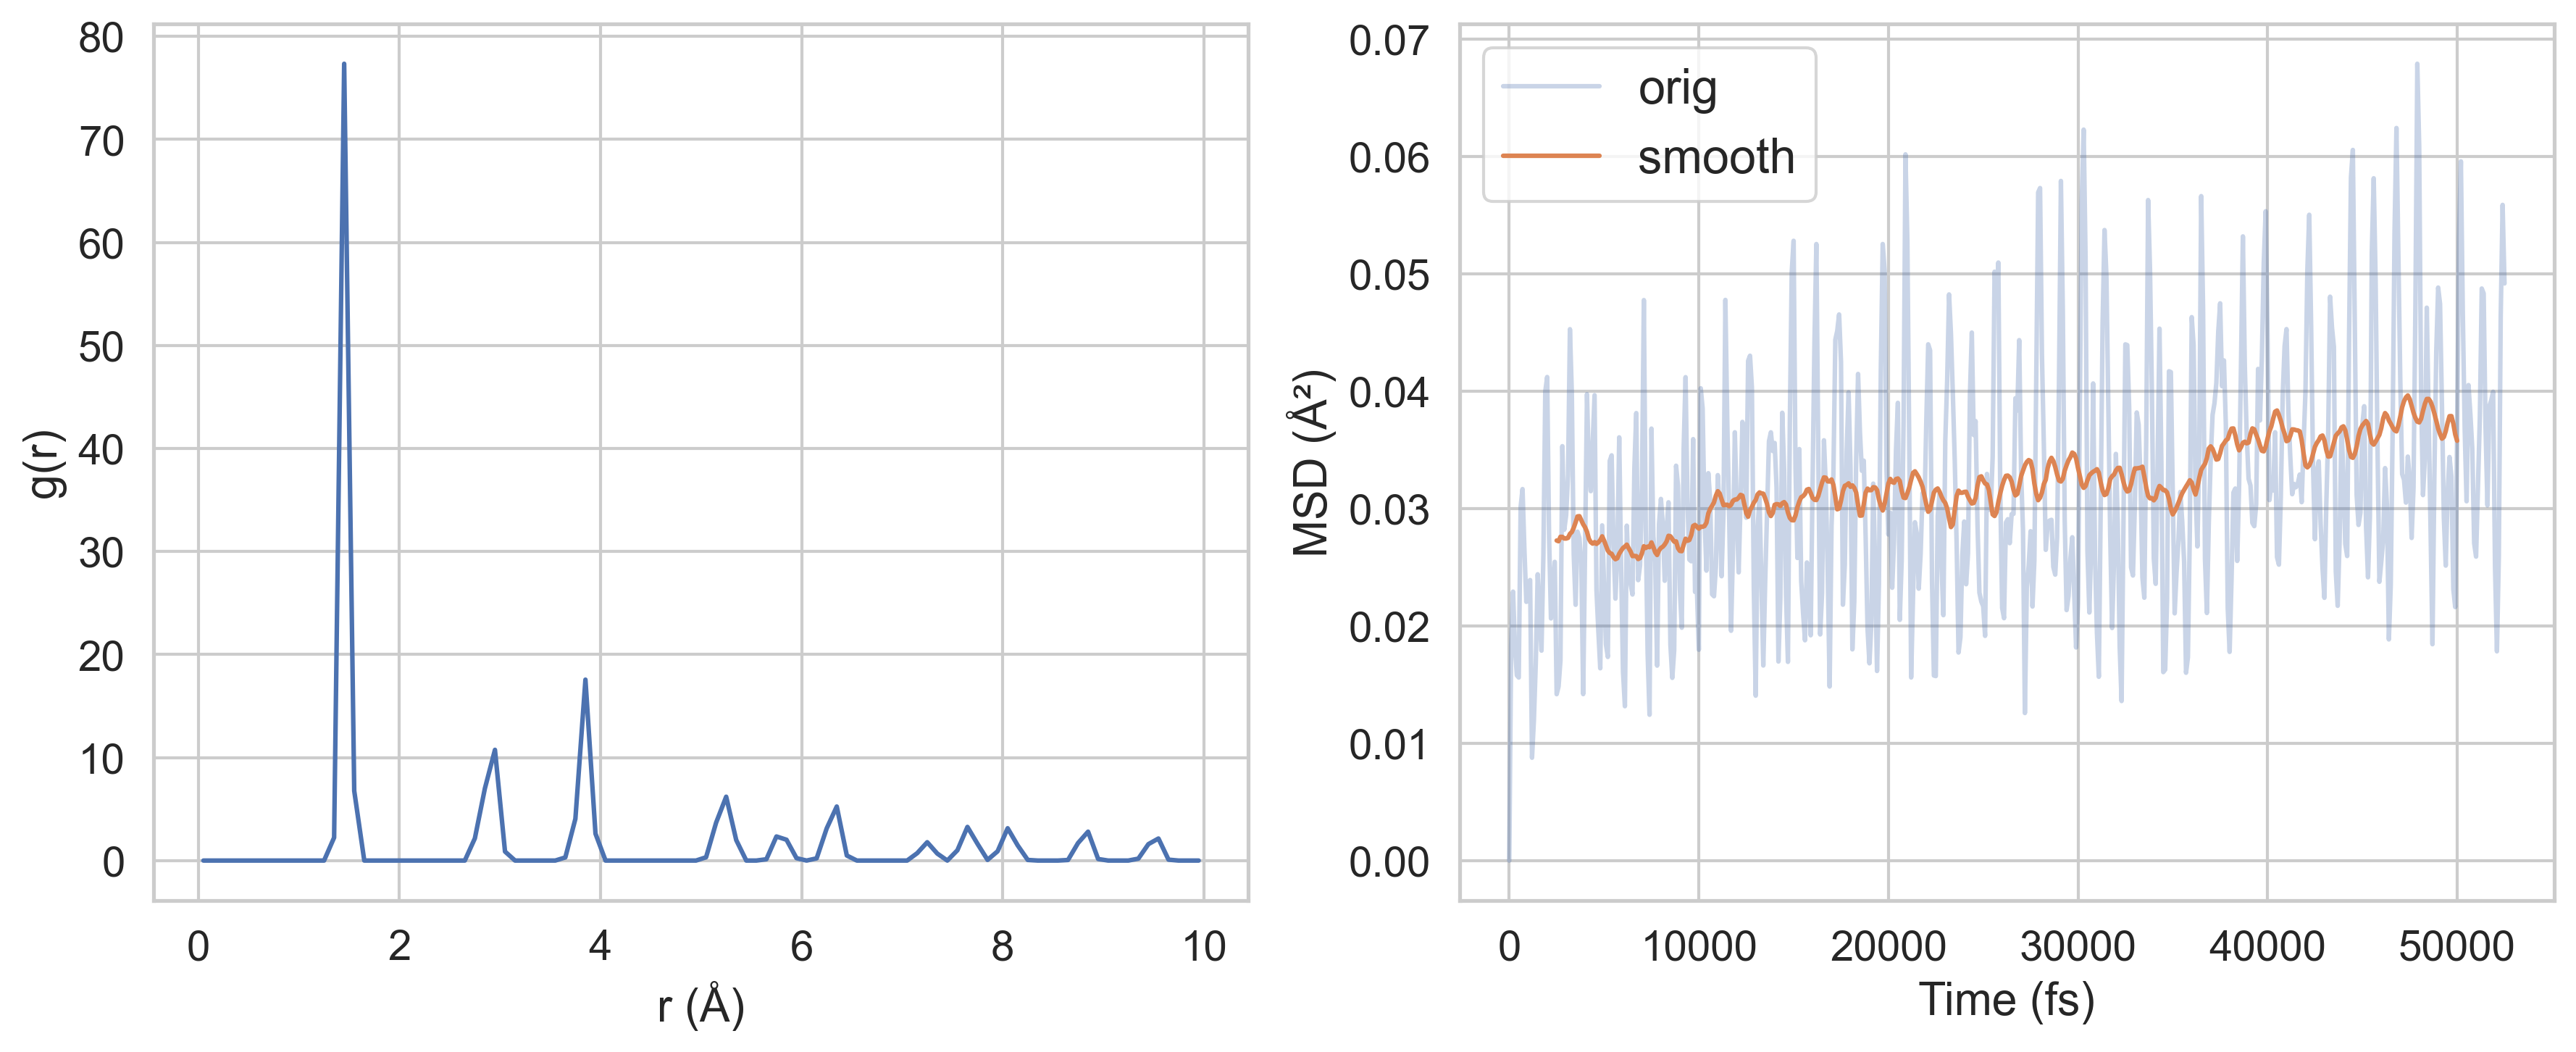
\includegraphics[width=\linewidth]{pure_800K_notitle.png}
    \caption{Murni, 800 K}
    \label{subfig:rdf_msd_pure_800k}
  \end{subfigure}
  \vspace{1em}
  \begin{subfigure}{0.9\textwidth}
    \centering
    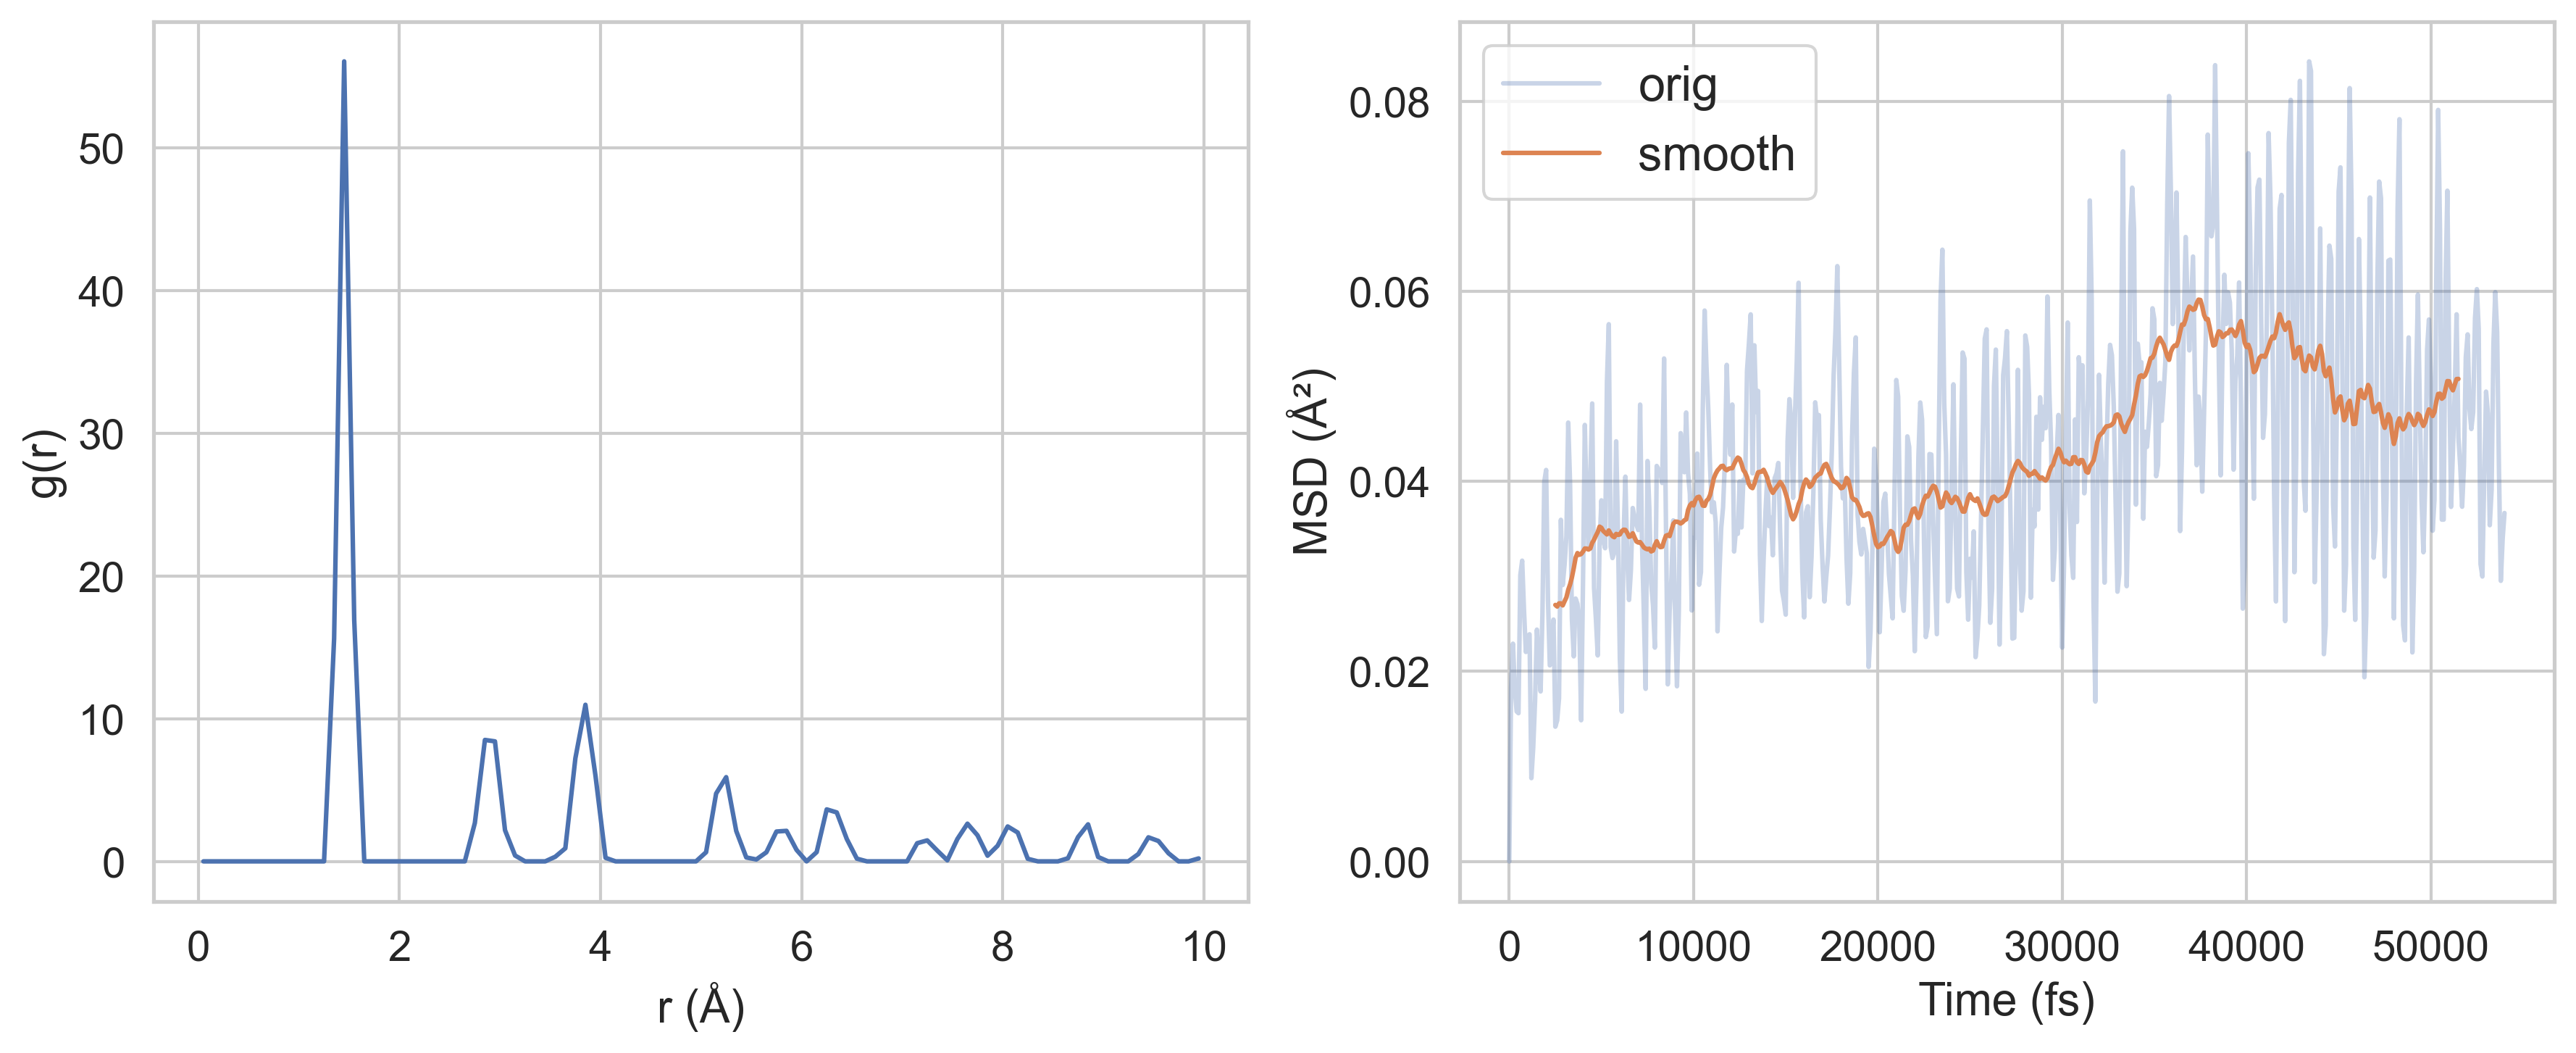
\includegraphics[width=\linewidth]{pure_1100K_notitle.png}
    \caption{Murni, 1100 K}
    \label{subfig:rdf_msd_pure_1100k}
  \end{subfigure}
  \vspace{1em}
  \begin{subfigure}{0.9\textwidth}
    \centering
    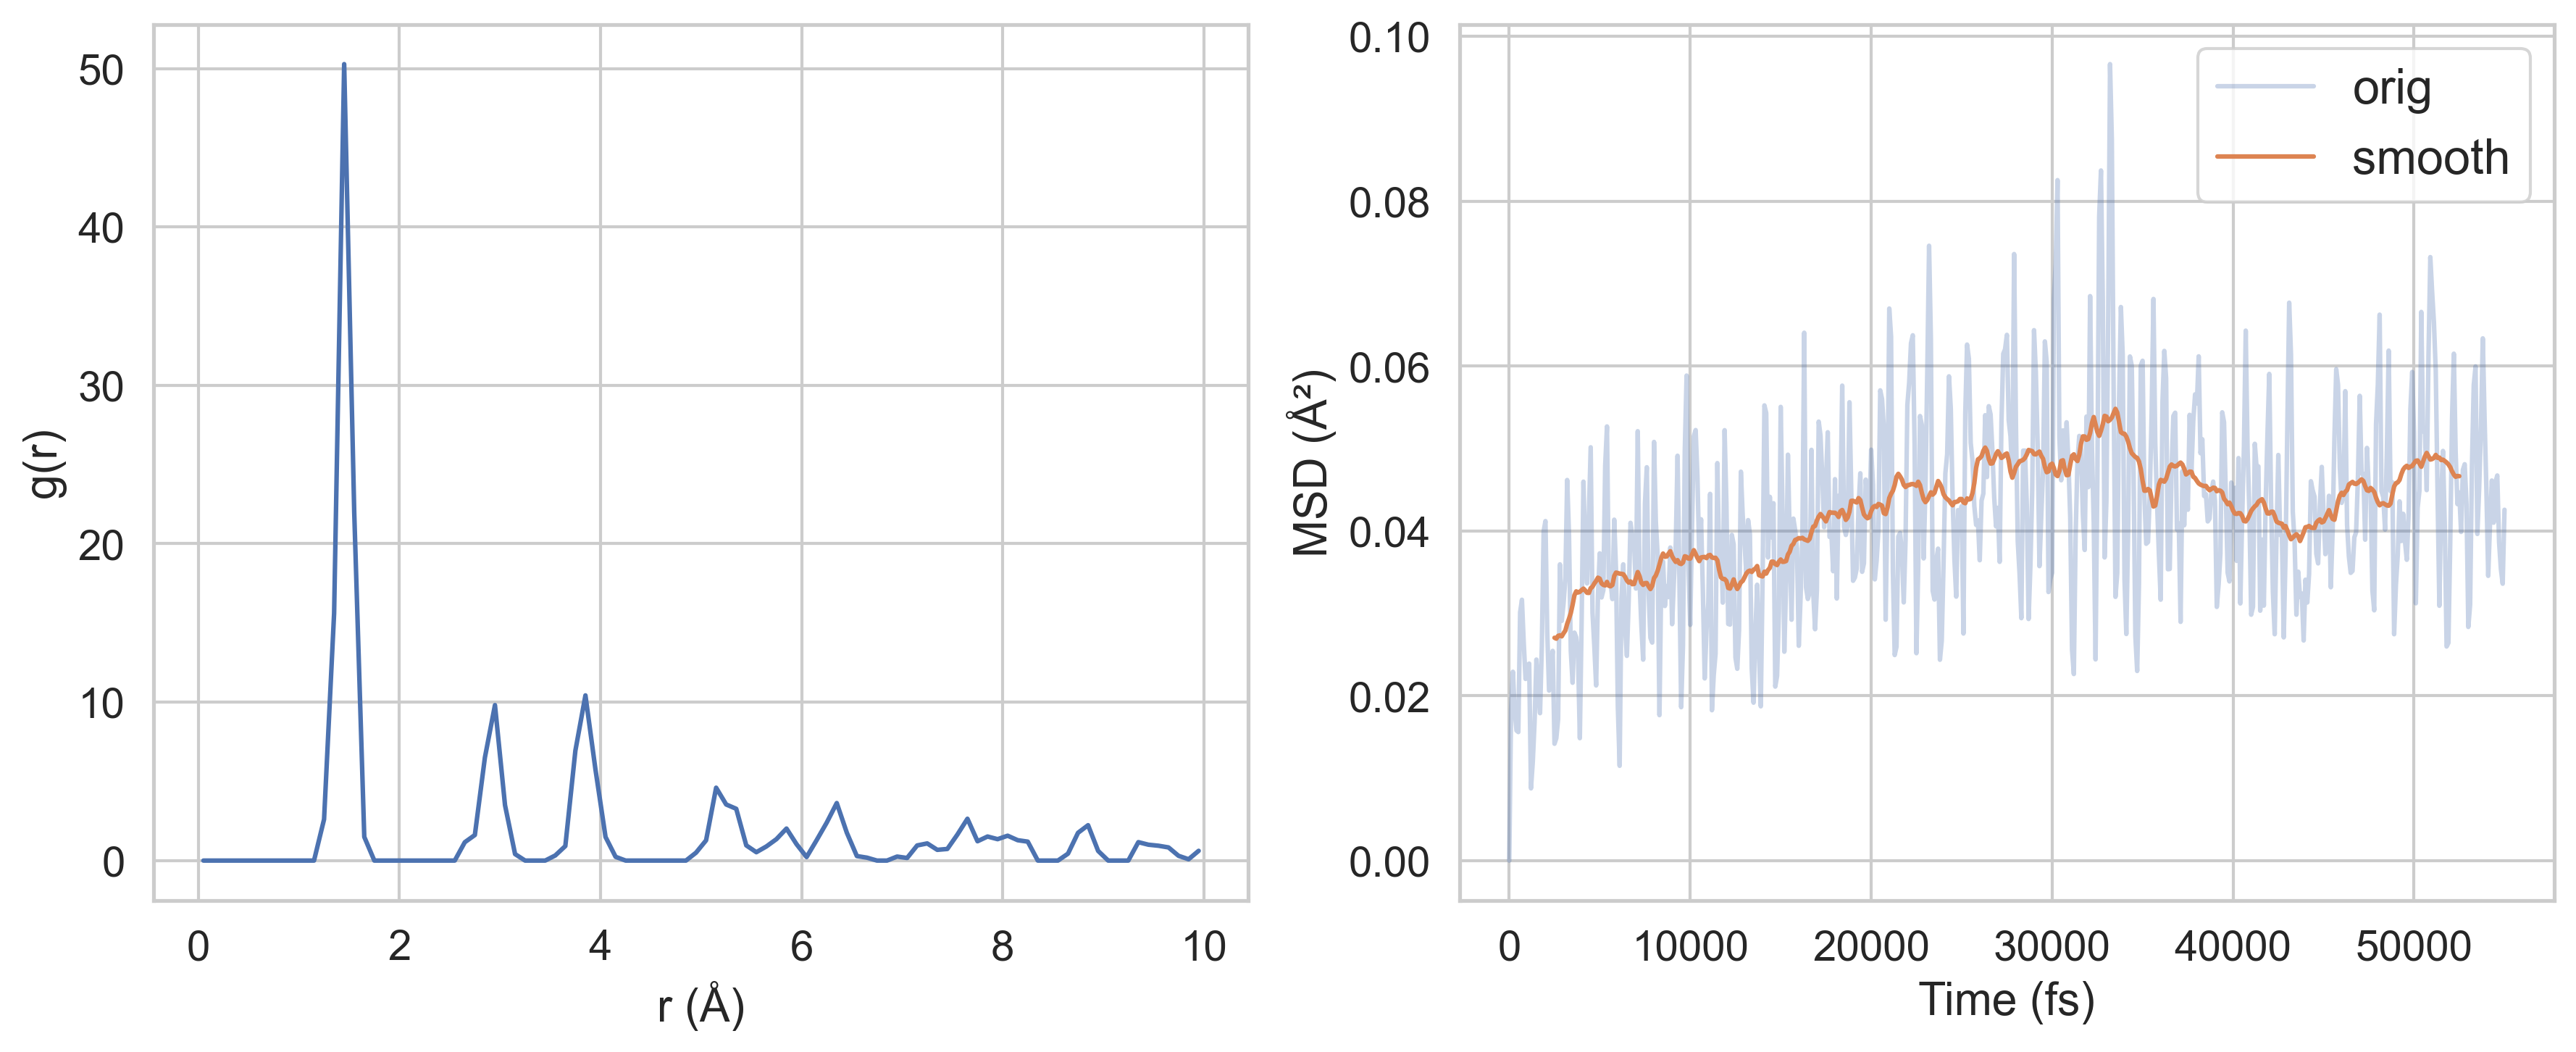
\includegraphics[width=\linewidth]{pure_1225K_notitle.png}
    \caption{Murni, 1225 K}
    \label{subfig:rdf_msd_pure_1225k}
  \end{subfigure}
  \label{fig:rdf_msd_grid}
\end{figure}

% --- Bagian 2: Cacat N_B ---
\begin{figure}[htbp]\ContinuedFloat
  \centering
  \begin{subfigure}{0.9\textwidth}
    \centering
    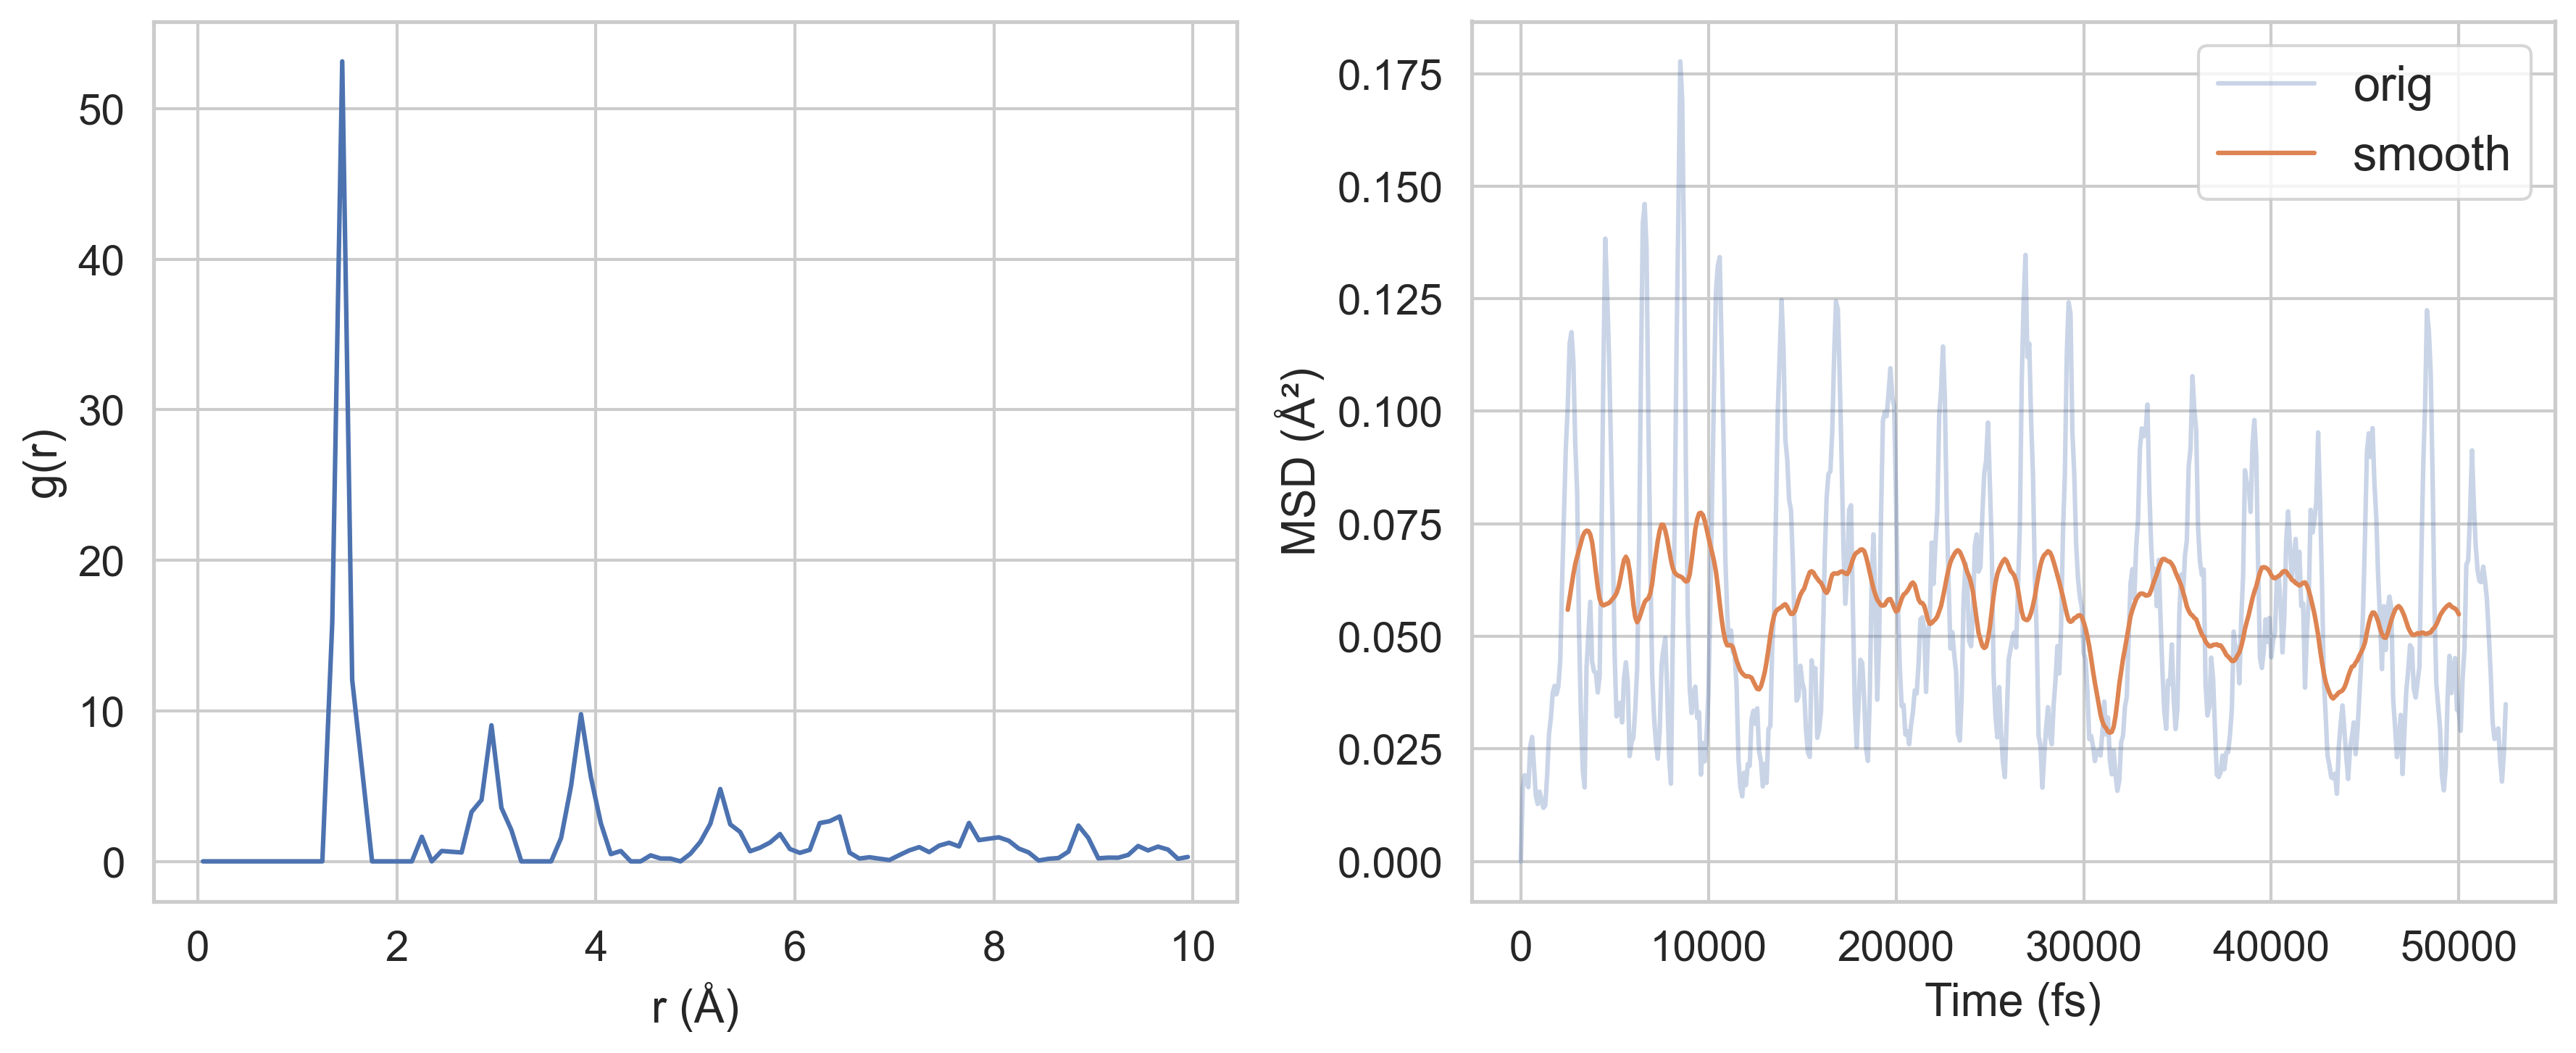
\includegraphics[width=\linewidth]{NN_800K_notitle.png}
    \caption{Cacat N\textsubscript{B}, 800 K}
    \label{subfig:rdf_msd_nn_800k}
  \end{subfigure}
  \vspace{1em}
  \begin{subfigure}{0.9\textwidth}
    \centering
    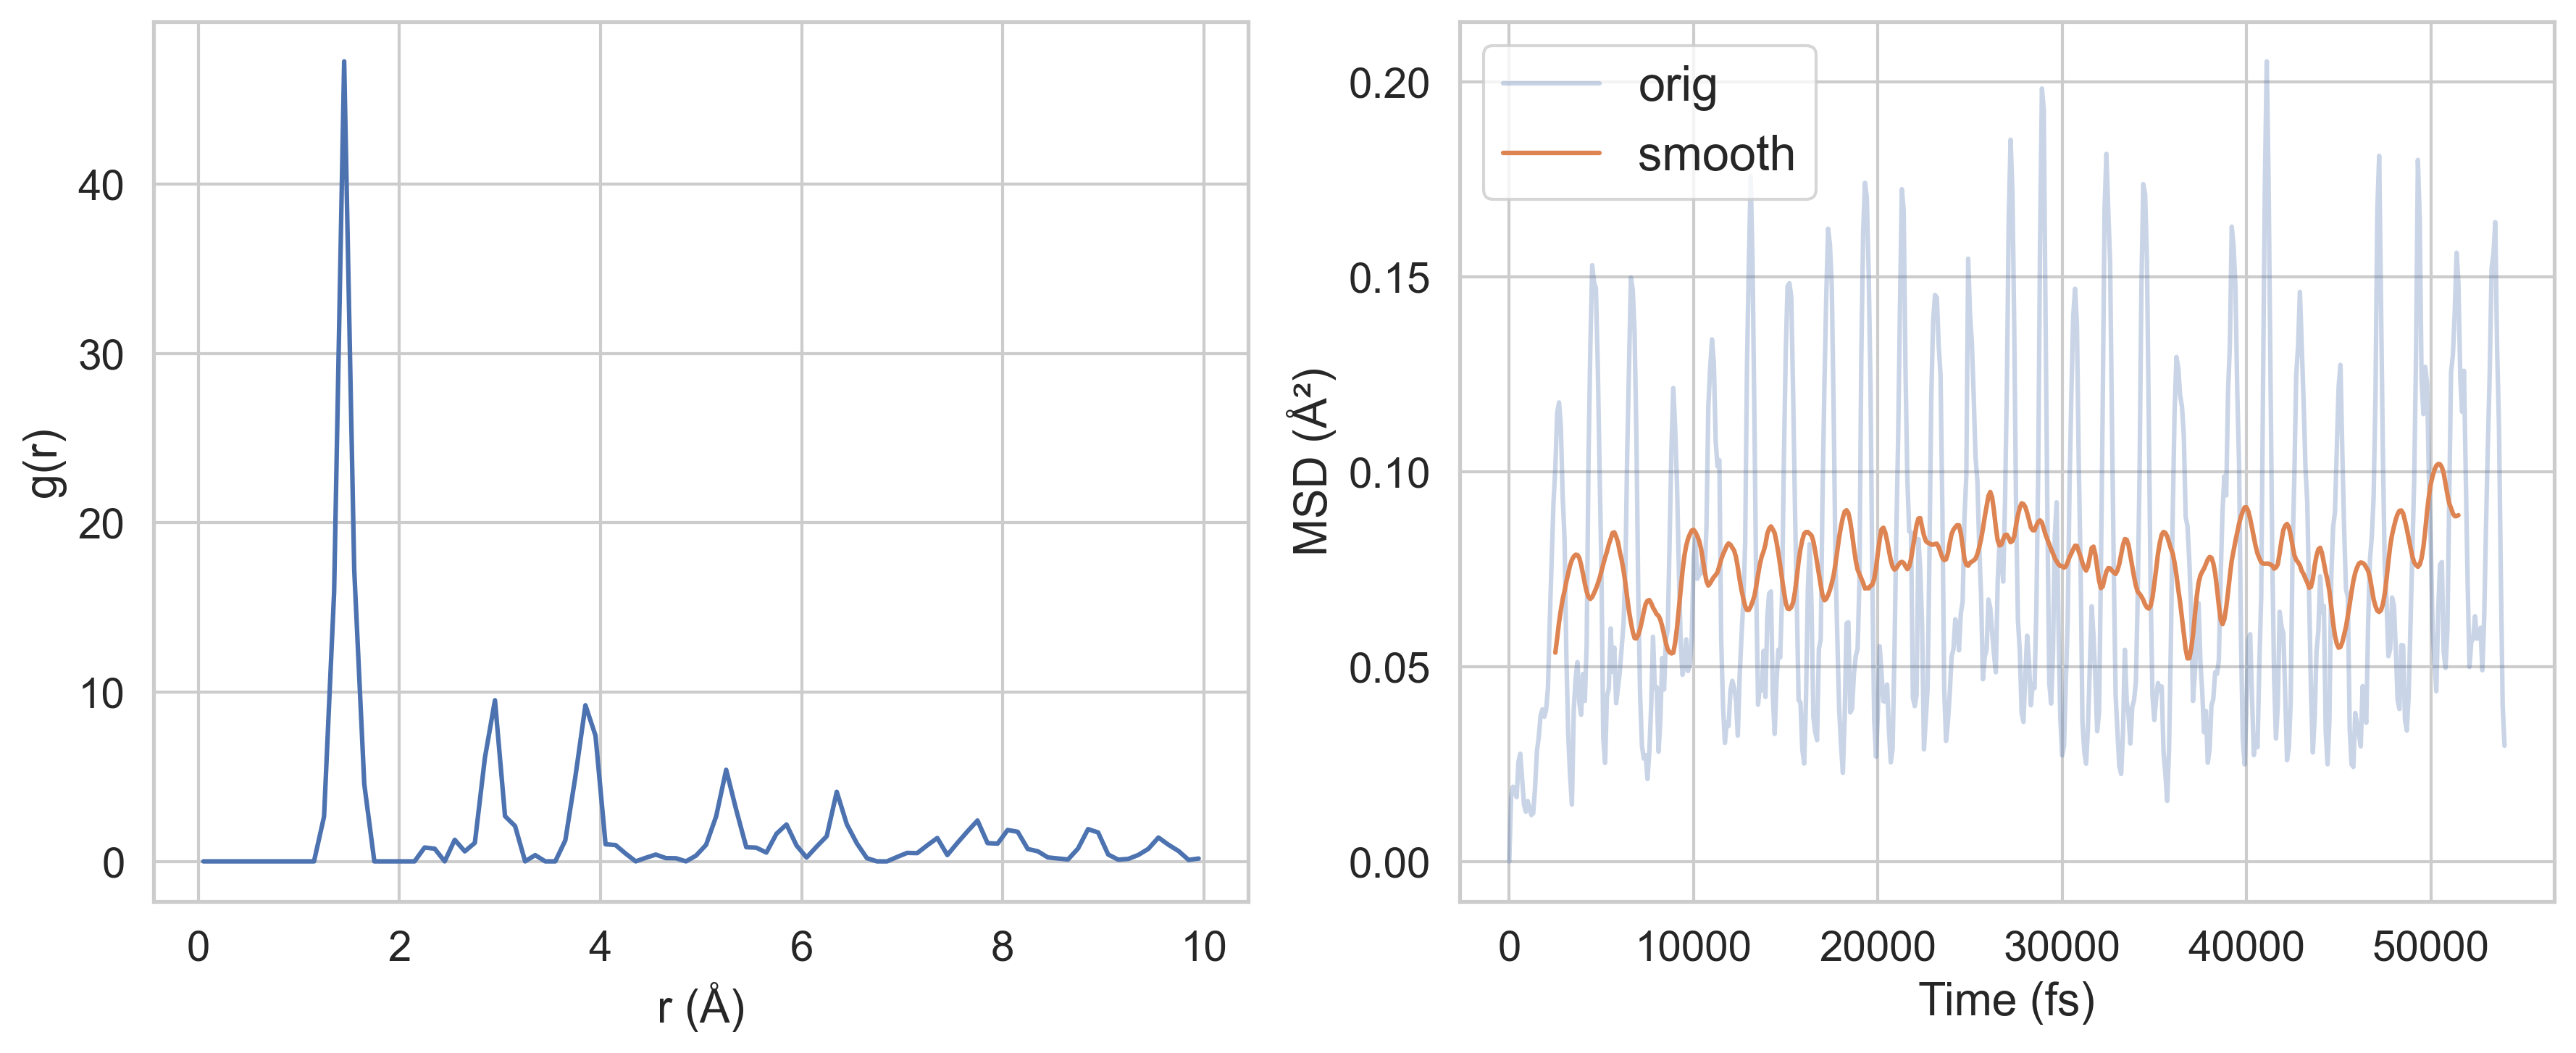
\includegraphics[width=\linewidth]{NN_1100K_notitle.png}
    \caption{Cacat N\textsubscript{B}, 1100 K}
    \label{subfig:rdf_msd_nn_1100k}
  \end{subfigure}
  \vspace{1em}
  \begin{subfigure}{0.9\textwidth}
    \centering
    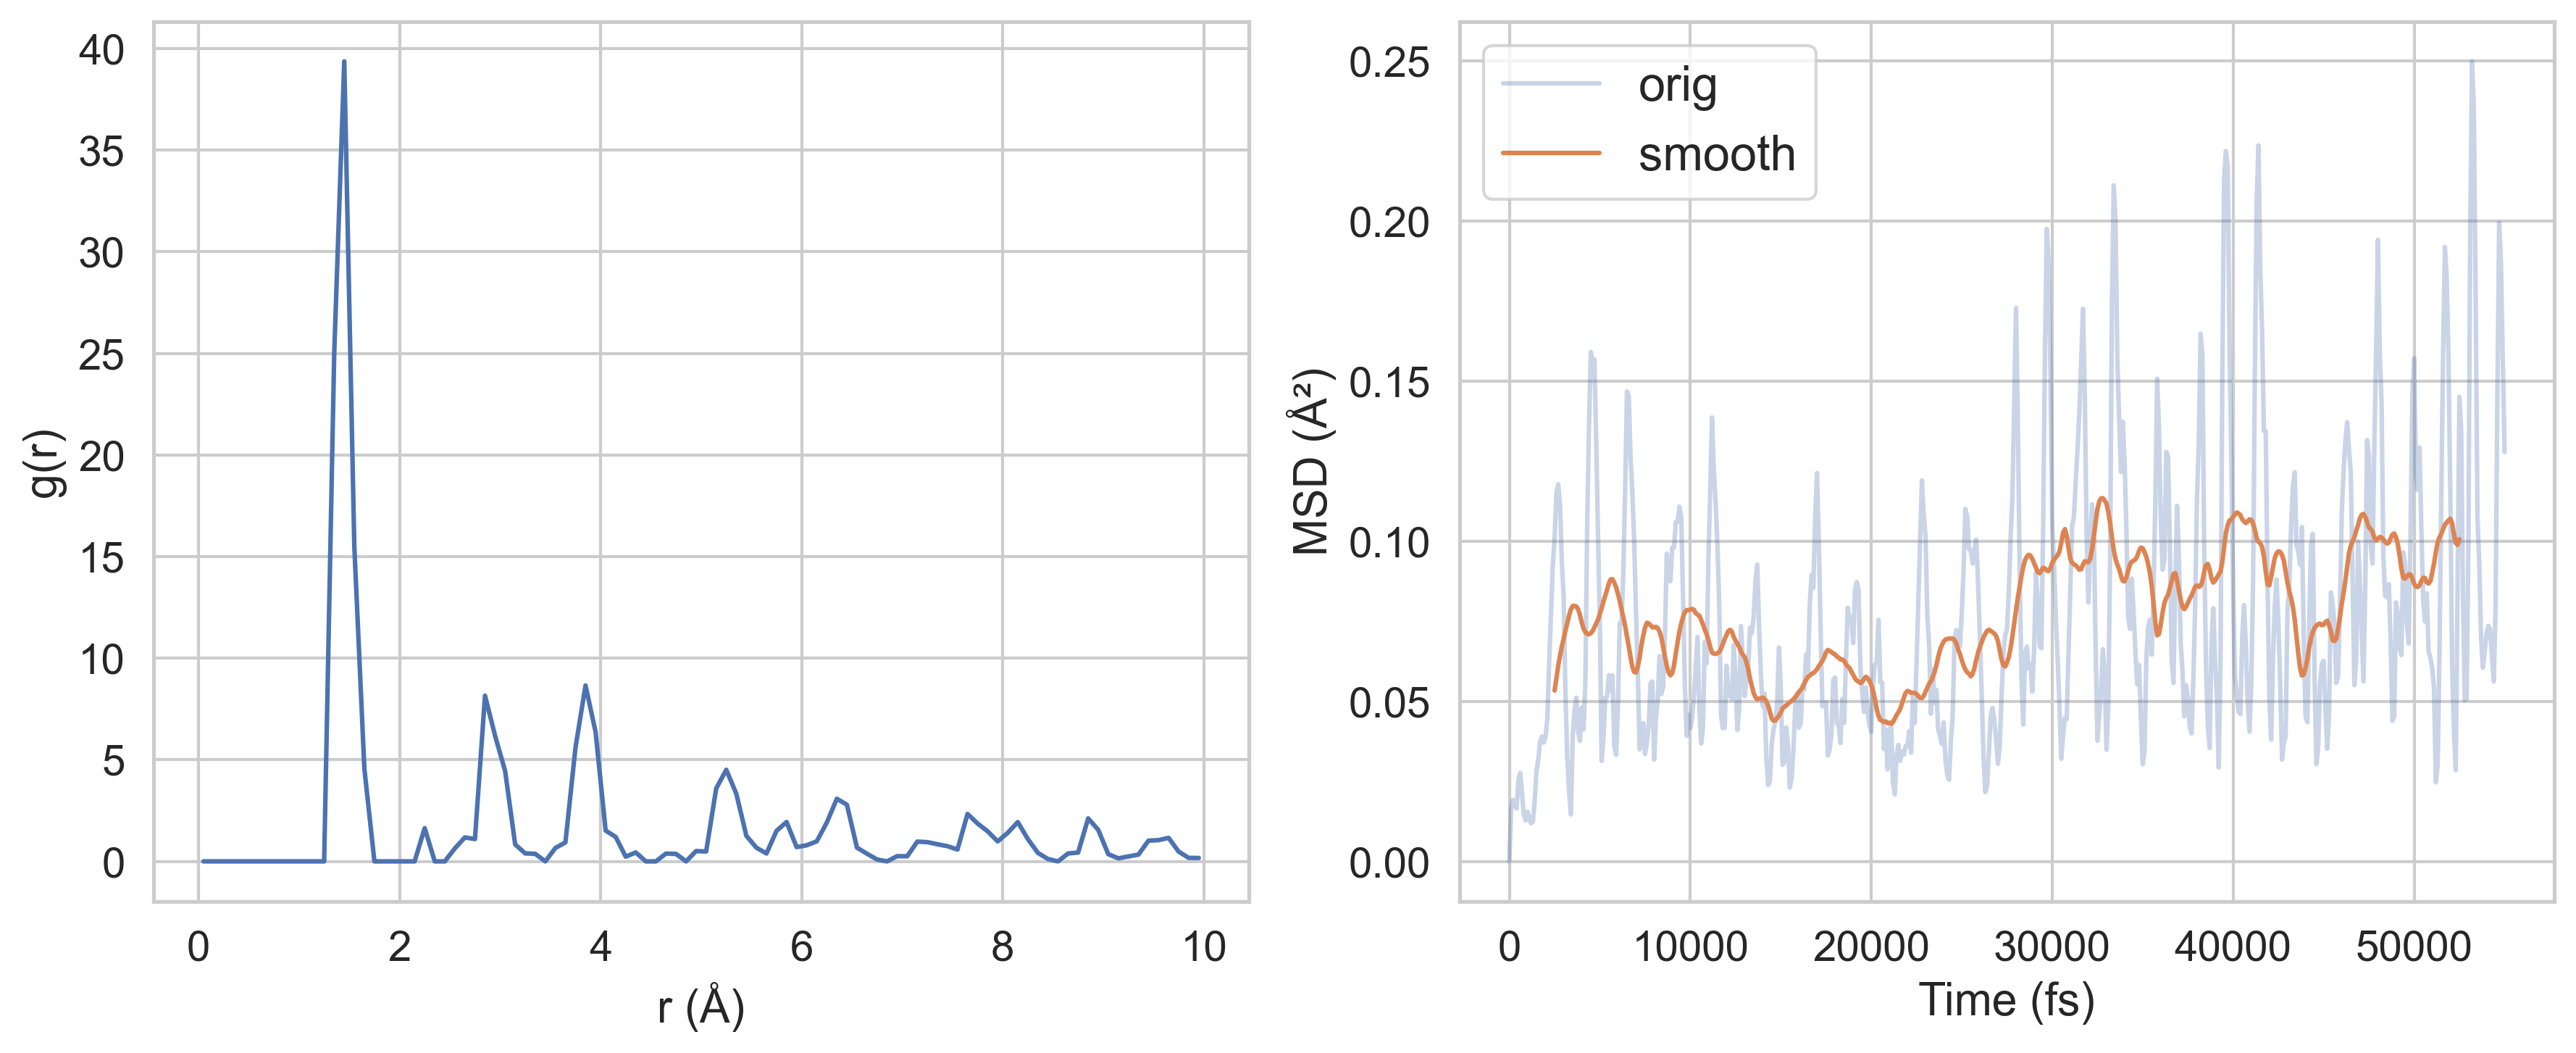
\includegraphics[width=\linewidth]{NN_1225K_notitle.png}
    \caption{Cacat N\textsubscript{B}, 1225 K}
    \label{subfig:rdf_msd_nn_1225k}
  \end{subfigure}
\end{figure}

% --- Bagian 3: Cacat B_N ---
\begin{figure}[htbp]\ContinuedFloat
  \centering
  \begin{subfigure}{0.9\textwidth}
    \centering
    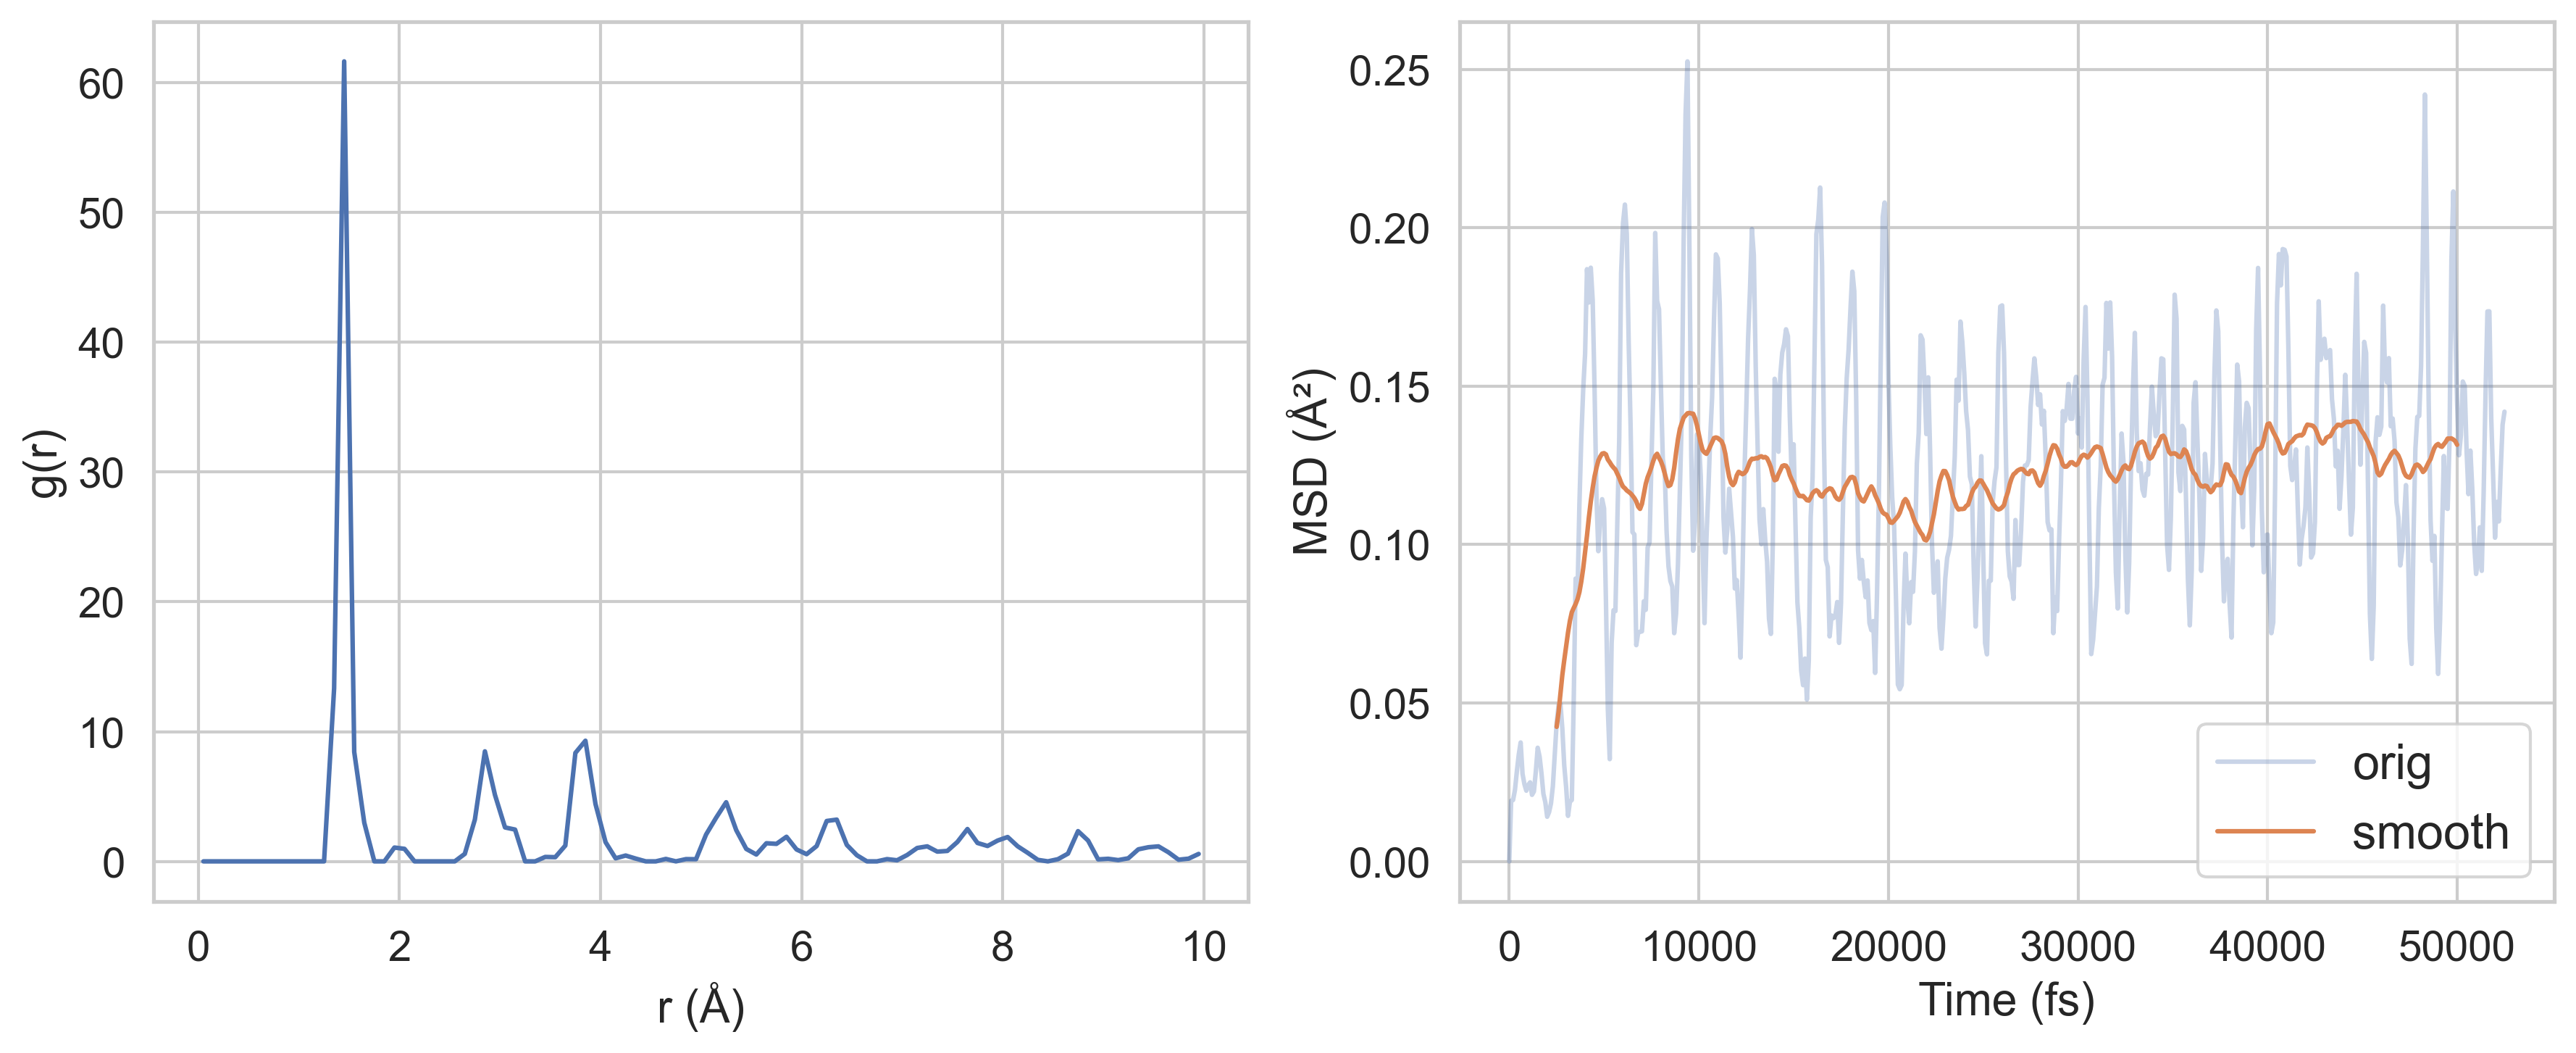
\includegraphics[width=\linewidth]{BB_800K_notitle.png}
    \caption{Cacat B\textsubscript{N}, 800 K}
    \label{subfig:rdf_msd_bb_800k}
  \end{subfigure}
  \vspace{1em}
  \begin{subfigure}{0.9\textwidth}
    \centering
    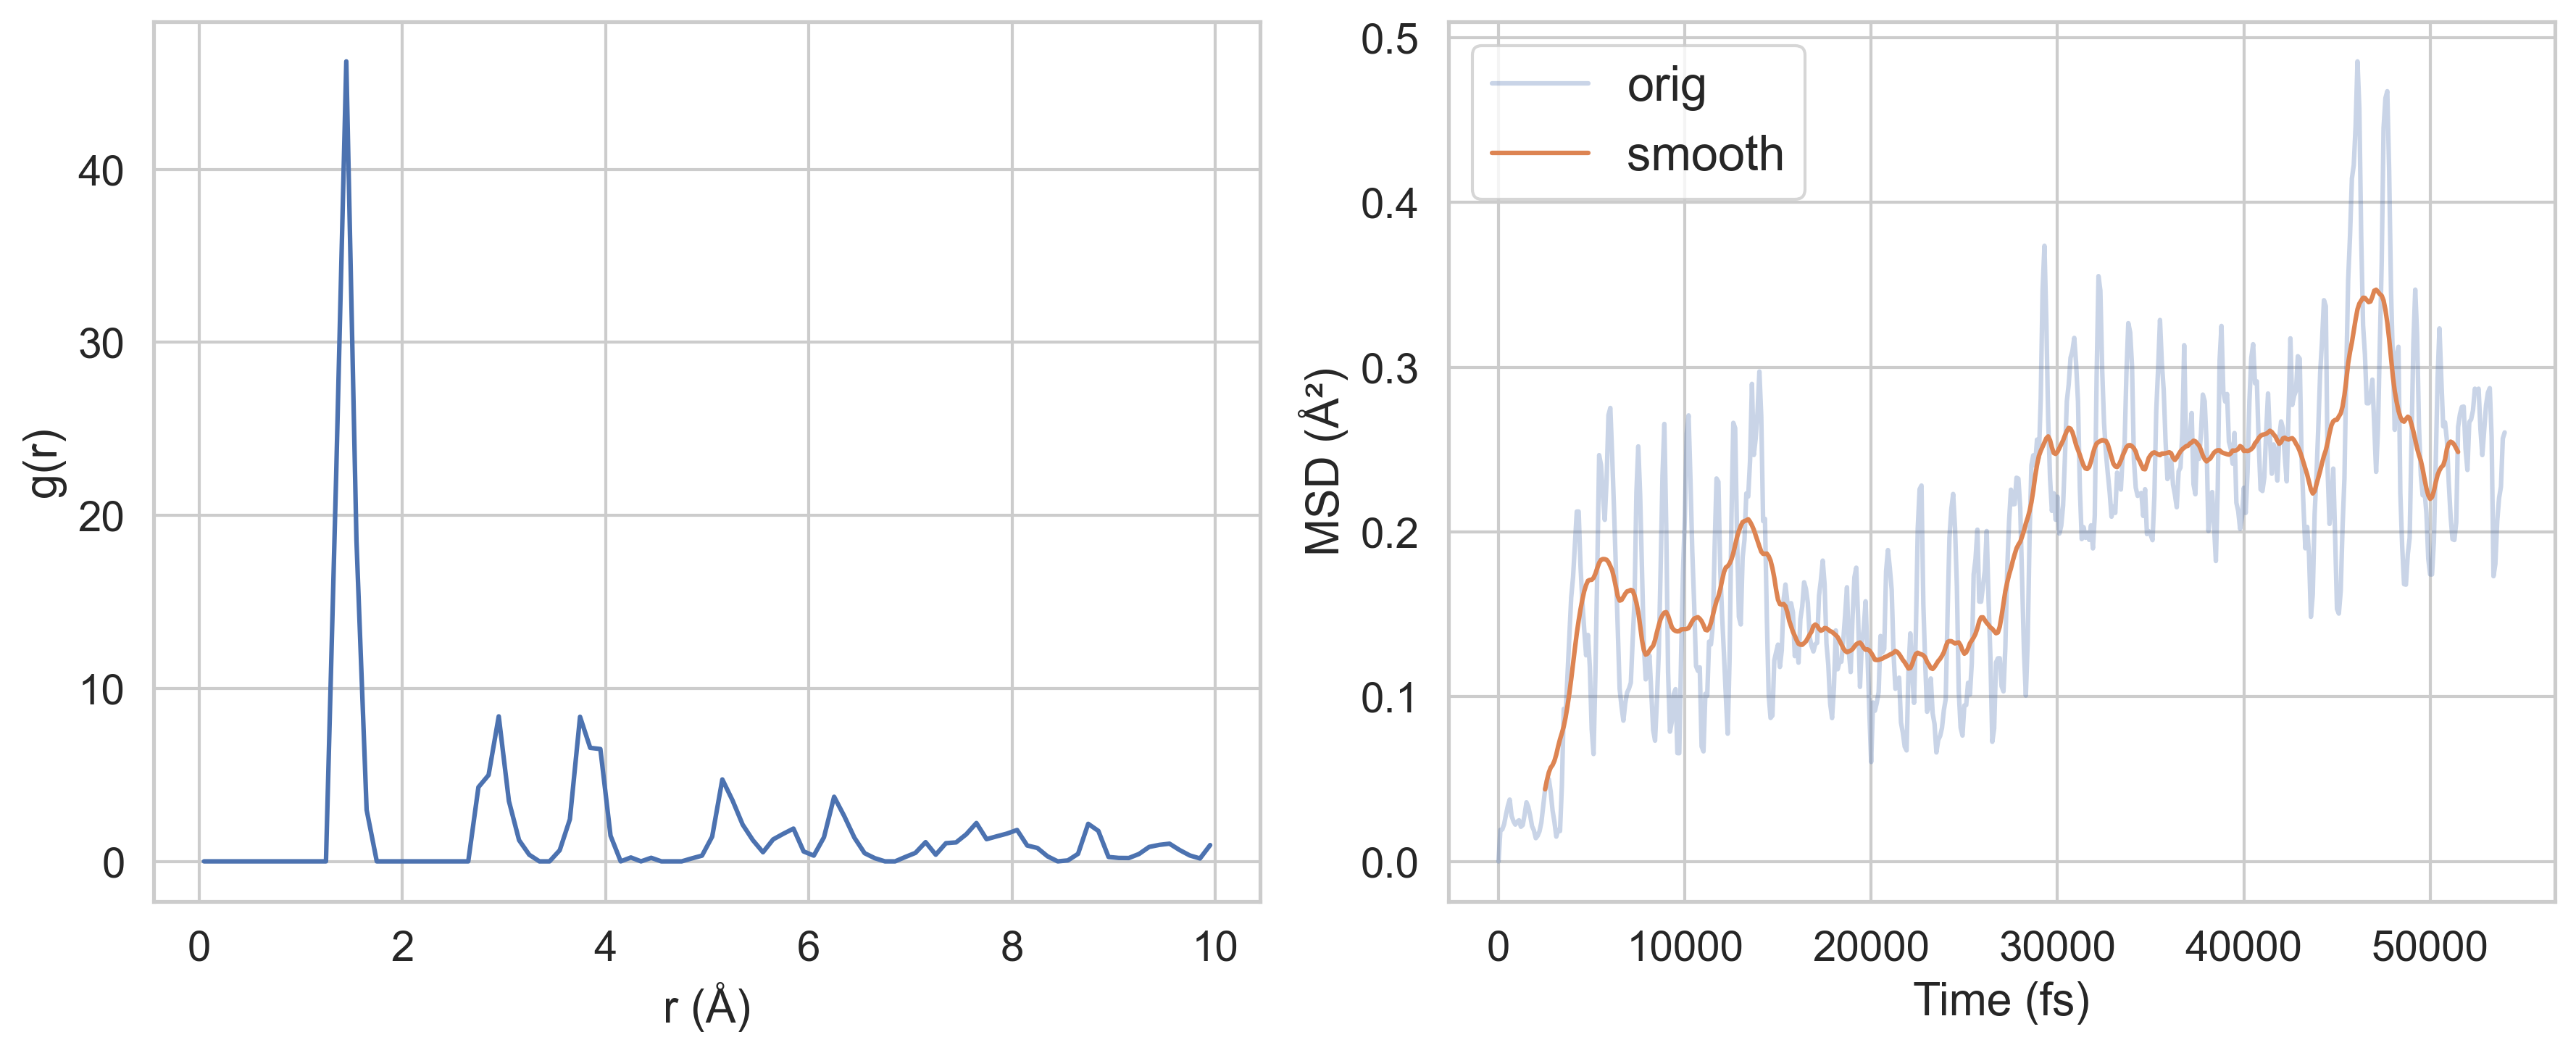
\includegraphics[width=\linewidth]{BB_1100K_notitle.png}
    \caption{Cacat B\textsubscript{N}, 1100 K}
    \label{subfig:rdf_msd_bb_1100k}
  \end{subfigure}
  \vspace{1em}
  \begin{subfigure}{0.9\textwidth}
    \centering
    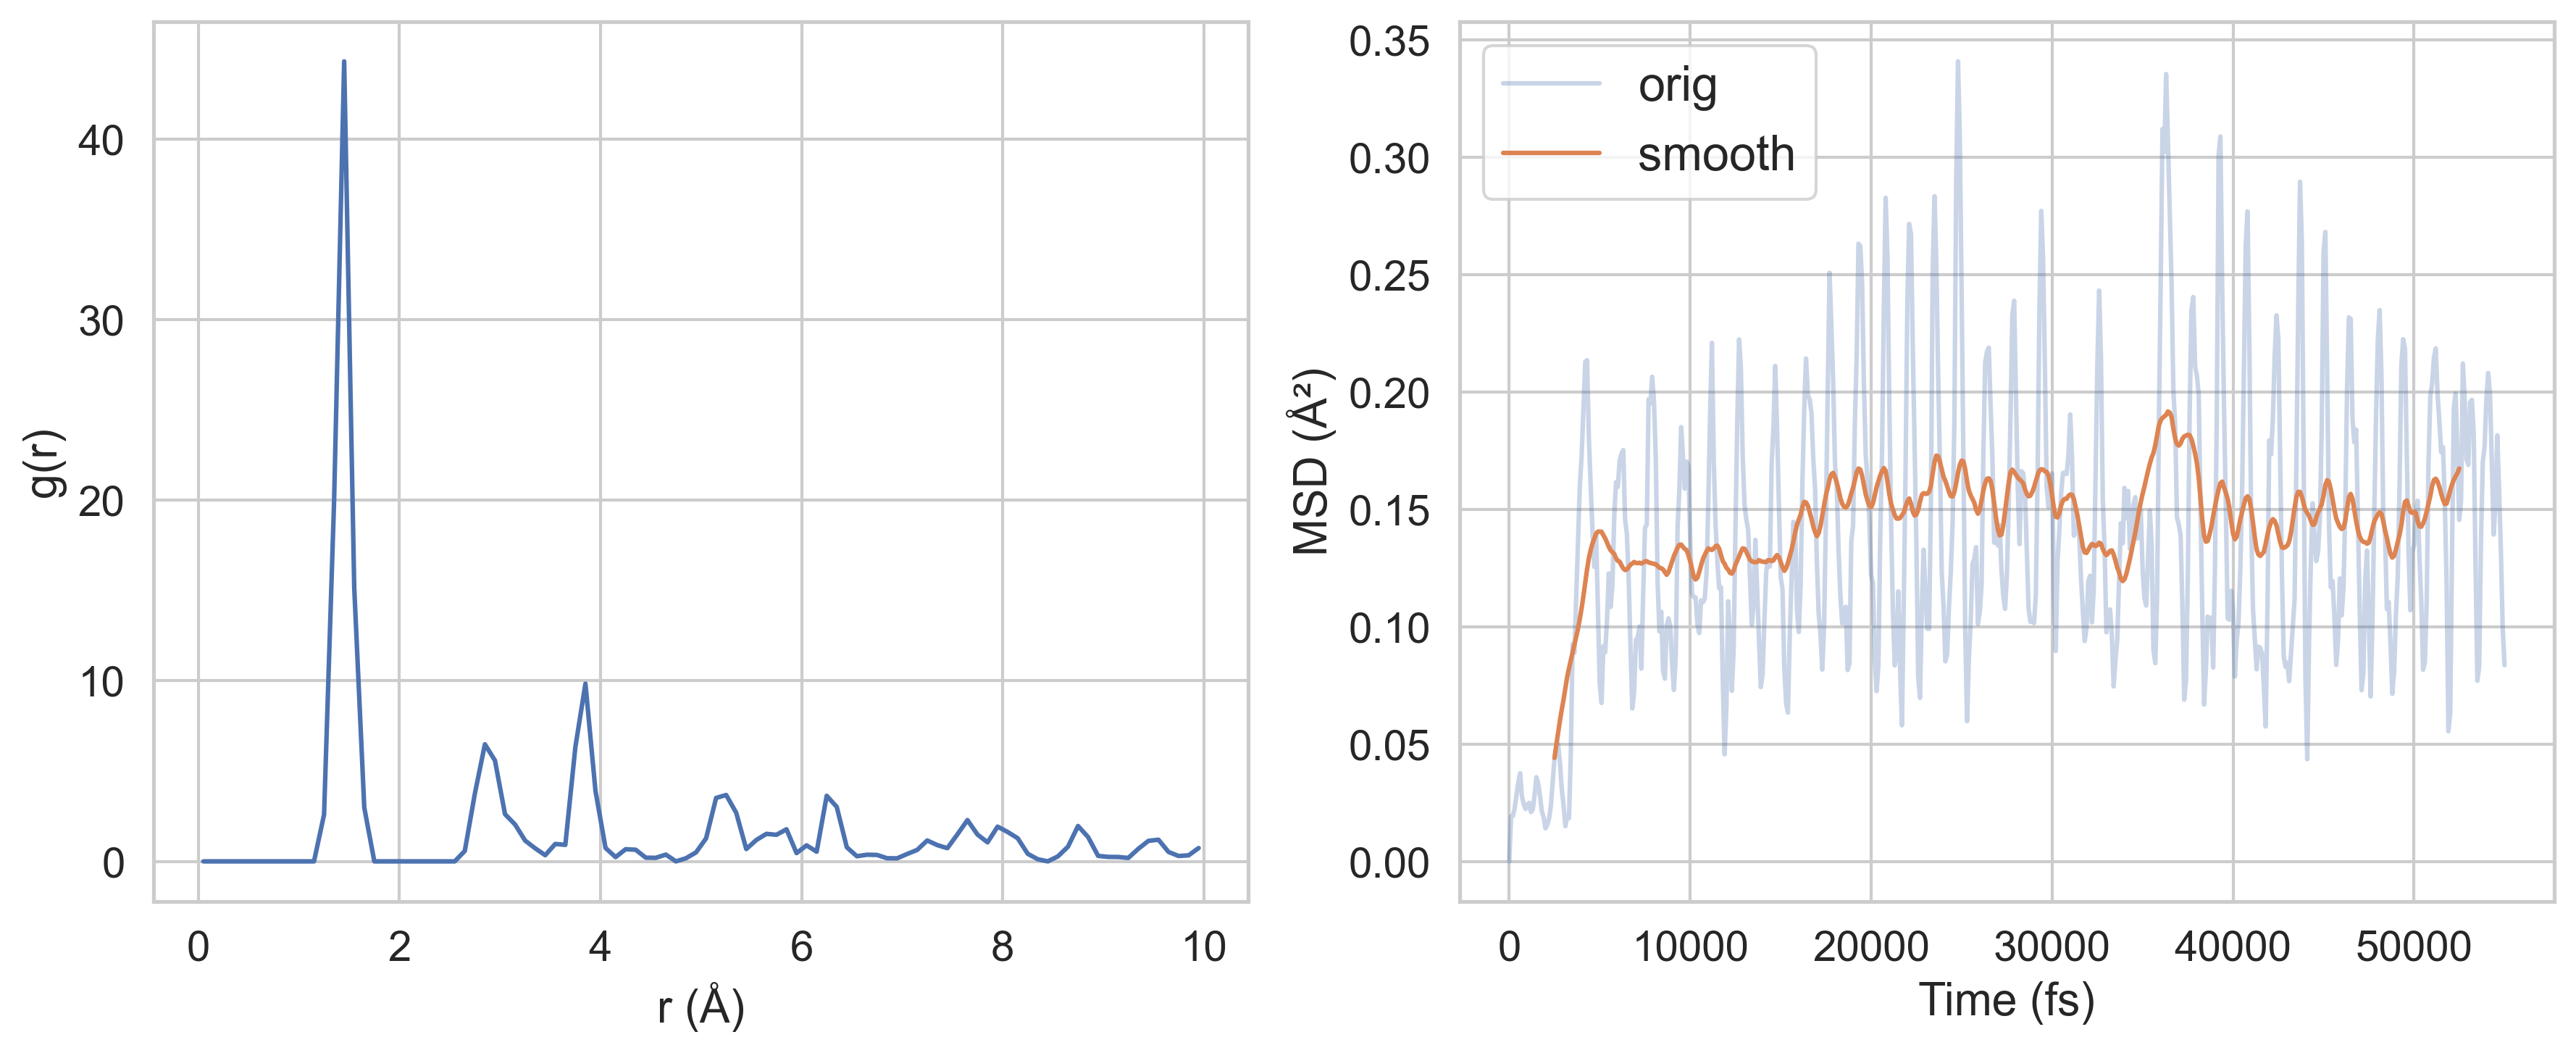
\includegraphics[width=\linewidth]{BB_1225K_notitle.png}
    \caption{Cacat B\textsubscript{N}, 1225 K}
    \label{subfig:rdf_msd_bb_1225k}
  \end{subfigure}
    \caption{Plot RDF dan MSD untuk setiap variasi}
\end{figure}

Gambar \ref{fig:rdf_msd_grid} menunjukkan plot RDF dan MSD untuk setiap sistem dan temperatur.
Beberapa tren kunci dapat diidentifikasi dari plot RDF:
\begin{itemize}
    \item Pengaruh Temperatur: Untuk semua sistem, seiring dengan meningkatnya temperatur dari 800 K ke 1225 K, puncak-puncak RDF menjadi lebih rendah dan lebih lebar.
Ini adalah indikasi klasik dari peningkatan gangguan termal (\emph{thermal disorder}).
Amplitudo vibrasi atom yang lebih besar menyebabkan distribusi jarak antar-atom yang lebih luas, sehingga mengurangi korelasi posisi jarak jauh dan "melelehkan" puncak-puncak yang tajam.
\item Pengaruh Cacat: Pada temperatur yang sama, sistem dengan cacat (N\textsubscript{B} dan B\textsubscript{N}) umumnya menunjukkan puncak yang sedikit lebih lebar dibandingkan sistem murni.
Ini mengindikasikan bahwa cacat mengintroduksi gangguan struktural statis di atas gangguan termal dinamis.
Kehadiran ikatan yang "salah" (misalnya, B-B atau N-N di sekitar cacat antisite) dan relaksasi kisi lokal di sekitarnya memutus periodisitas sempurna dan mengurangi tatanan kristal.
Sistem B\textsubscript{N} menunjukkan pelebaran puncak yang paling signifikan, menandakan distorsi lokal terbesar, yang merupakan prasyarat penting untuk fenomena elektronik yang akan dibahas nanti.
\end{itemize}

Dari plot MSD pada Gambar \ref{fig:rdf_msd_grid}, perilaku dinamis sistem dapat dianalisis:
\begin{itemize}
    \item Stabilitas Fasa Padat: Untuk semua kasus, MSD meningkat seiring waktu tetapi tidak menunjukkan rezim difusif linier yang jelas (seperti pada cairan), melainkan menunjukkan perilaku sub-difusif yang khas untuk atom dalam fasa padat pada temperatur tinggi.
Ini mengonfirmasi bahwa monolayer hBN, bahkan pada 1225 K, tetap dalam keadaan padat dan tidak meleleh selama simulasi.
\item Mobilitas Termal: Kemiringan kurva MSD secara kualitatif terkait dengan mobilitas atom.
Semakin curam kemiringannya, semakin tinggi mobilitas atom dan semakin rendah stabilitas strukturalnya.
Terlihat jelas bahwa untuk setiap jenis sistem, MSD meningkat lebih cepat pada temperatur yang lebih tinggi, yang konsisten dengan eksitasi termal yang lebih besar.
\item Dampak Cacat pada Stabilitas: Perbandingan antar sistem pada temperatur tertinggi (1225 K) sangat informatif.
Sistem murni menunjukkan MSD terendah, menandakan stabilitas struktural tertinggi. Sistem N\textsubscript{B} menunjukkan mobilitas yang lebih tinggi.
Secara signifikan, sistem B\textsubscript{N} menunjukkan MSD tertinggi dengan selisih yang jelas.
Ini menyiratkan bahwa atom-atom dalam sistem dengan cacat B\textsubscript{N} adalah yang paling mobile dan strukturnya paling tidak stabil secara dinamis.
Mobilitas atomik yang tinggi ini adalah manifestasi makroskopis dari vibrasi kisi (fonon) beramplitudo besar.
Lingkungan yang sangat dinamis dan terdistorsi di sekitar cacat B\textsubscript{N} inilah yang menciptakan kondisi untuk kopling spin-fonon yang kuat, seperti yang akan dibahas pada Bagian \ref{subsec:hbn_defek_bn}.
\end{itemize}

\section{Pengaruh Temperatur pada Sifat Elektronik Monolayer hBN Murni}
\label{sec:hbn_murni}
Analisis terhadap sistem hBN murni berfungsi sebagai dasar untuk memahami bagaimana sifat elektronik intrinsik material merespons eksitasi termal, sebelum mempertimbangkan efek yang lebih kompleks dari cacat.
\subsection{Karakteristik Elektronik Dasar hBN Murni (Sistem Referensi)}
\label{subsec:hbn_murni_dasar}
Sebagai titik acuan, sifat elektronik monolayer hBN murni dalam kondisi \emph{pristine} (struktur ideal teroptimasi, mendekati 0 K) dianalisis terlebih dahulu.
Hasil kalkulasi DFT (Gambar \ref{fig:hbn_pristine_bs_pdos}) menunjukkan bahwa hBN murni adalah isolator celah pita lebar non-magnetik.
Struktur pita menunjukkan celah pita langsung (\emph{direct band gap}) sebesar $E_g = 4.446$ eV pada titik K di Zona Brillouin.
Analisis Kerapatan Keadaan Terproyeksi (PDOS) mengonfirmasi bahwa puncak pita valensi (VBM) didominasi oleh orbital N $2p_z$ (membentuk pita $\pi$), sedangkan dasar pita konduksi (CBM) didominasi oleh orbital B $2p_z$ (membentuk pita $\pi^*$), sesuai dengan literatur \citep{Sachs2011}.
Visualisasi kerapatan muatan (tidak ditampilkan) menunjukkan akumulasi elektron di sekitar atom nitrogen yang lebih elektronegatif, mengindikasikan ikatan B-N yang bersifat kovalen polar.
\begin{figure}[htbp!] % PERUBAHAN: Ukuran gambar diperbesar
    \centering
    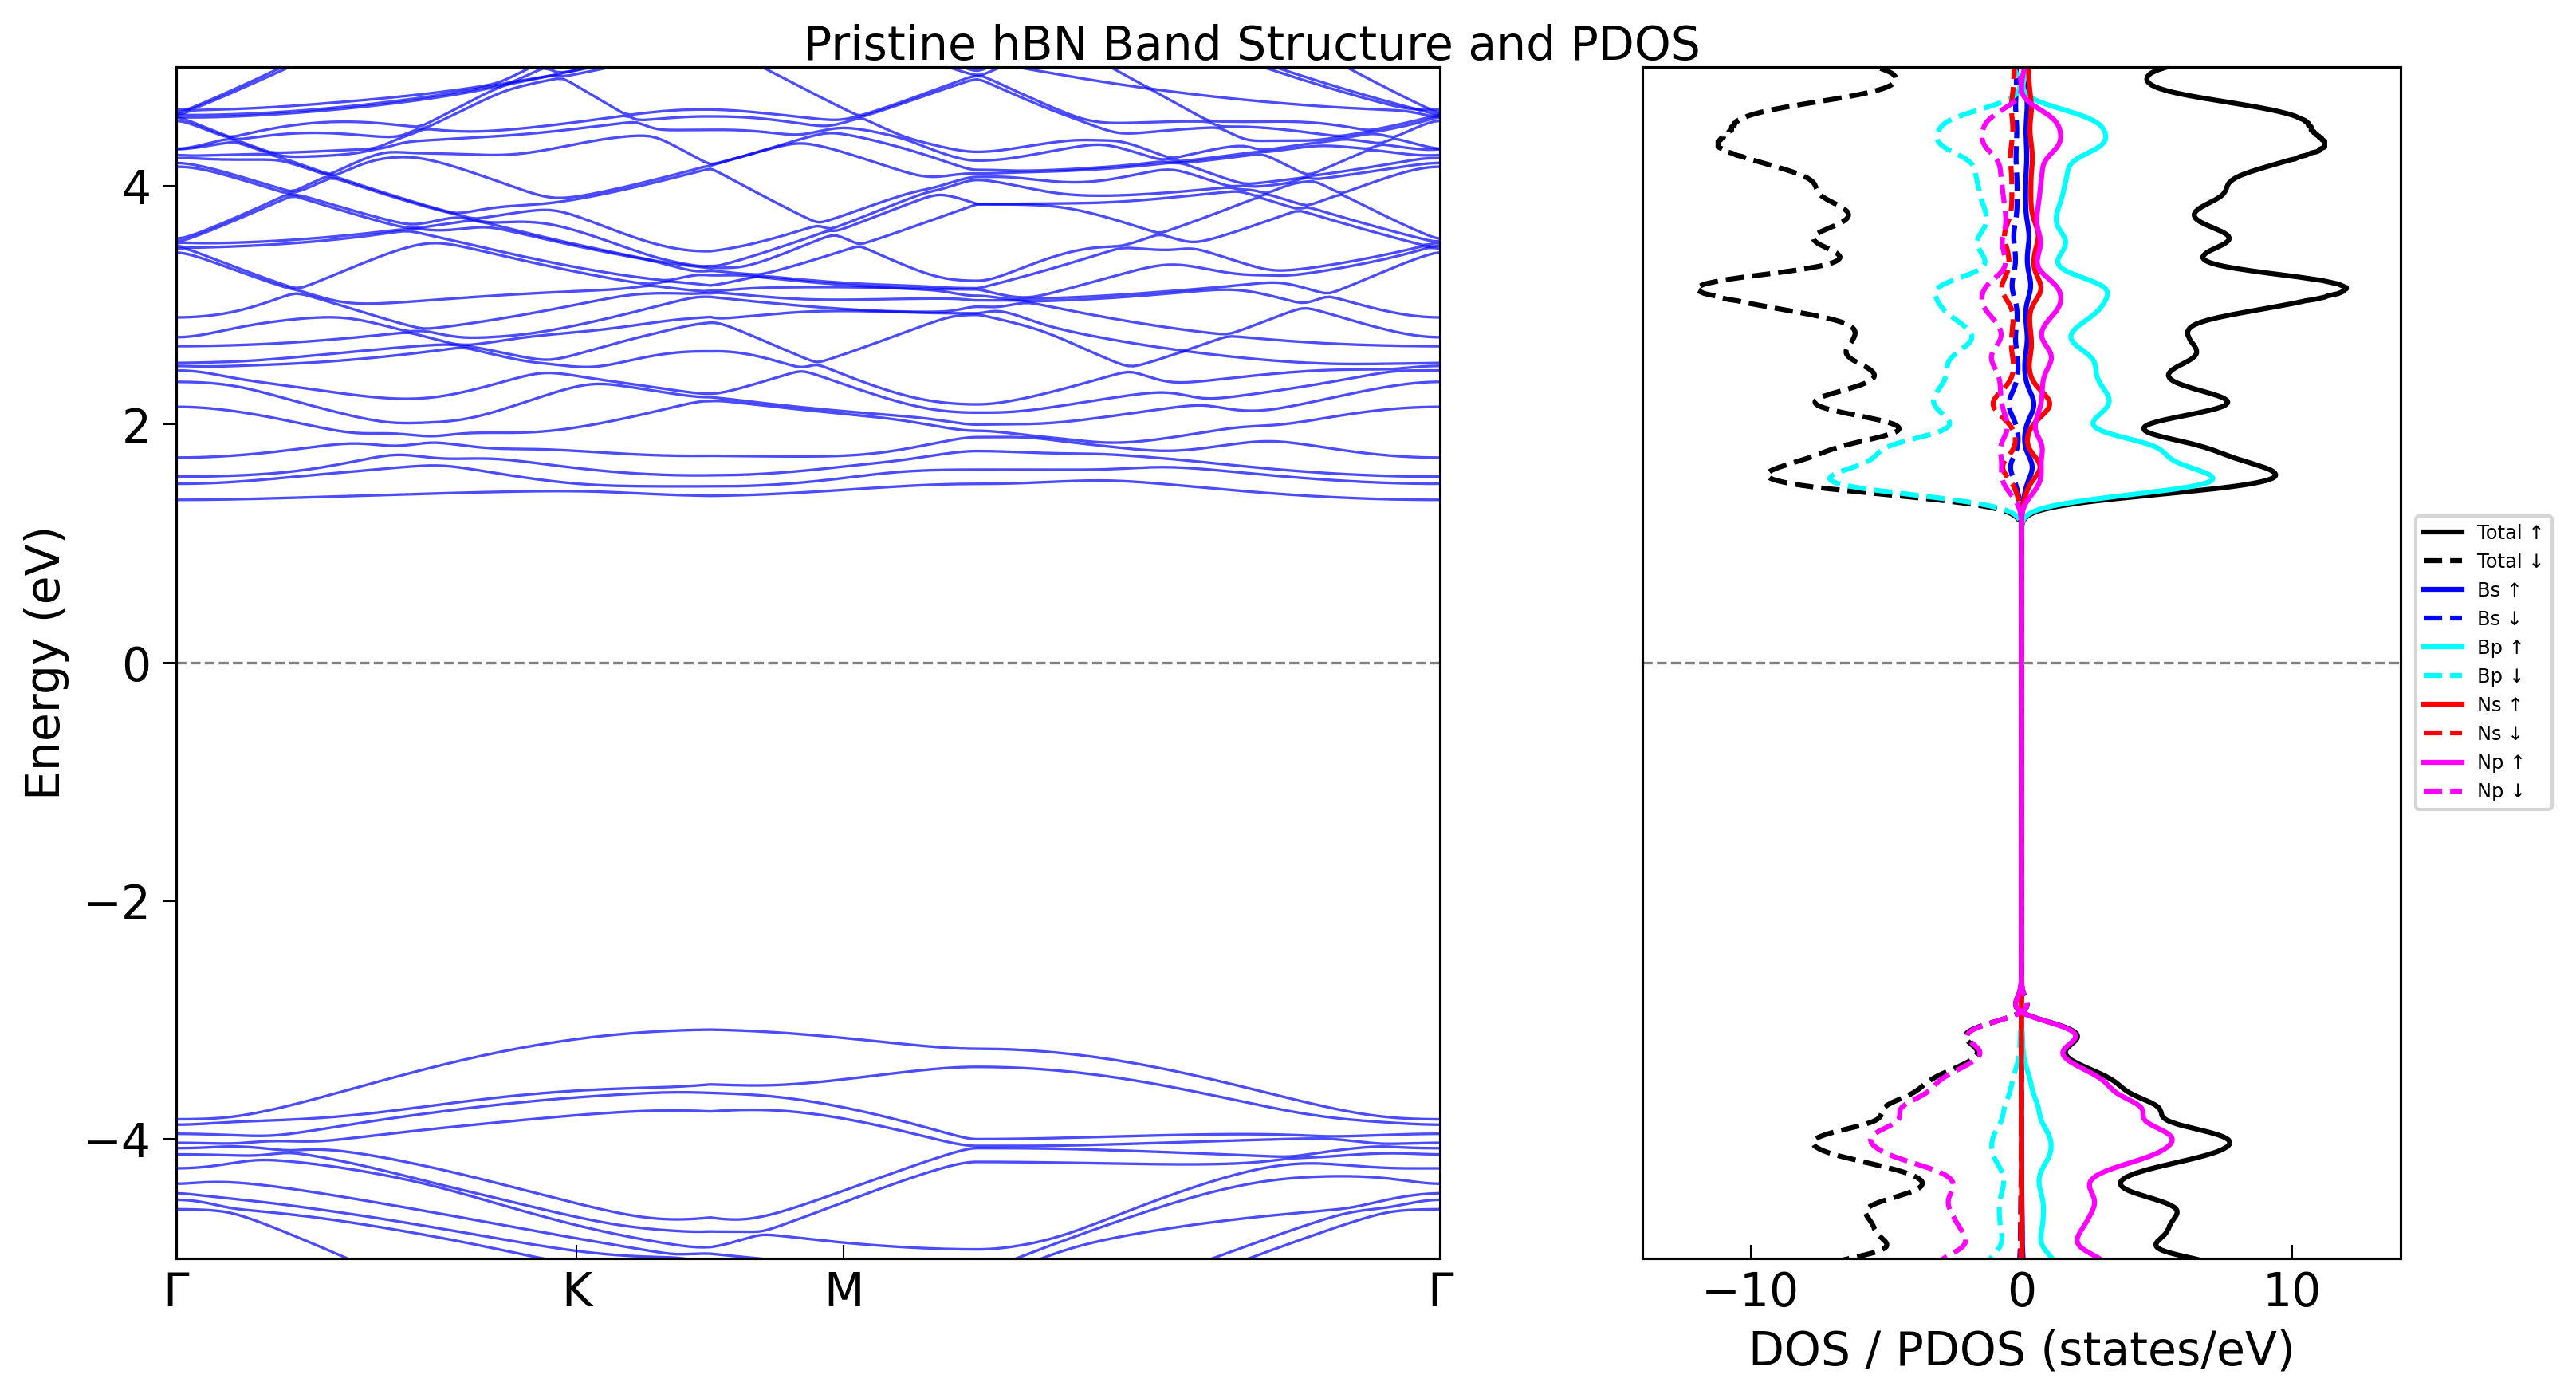
\includegraphics[width=0.95\textwidth]{gambar_hasil/simple_bands_pdos_pristine.png}
    \caption{Struktur pita elektronik dan Kerapatan Keadaan Terproyeksi (PDOS) untuk monolayer hBN murni (\emph{pristine}).
Energi Fermi ($E_F = -0.445$ eV) diset sebagai referensi energi nol pada plot PDOS.}
    \label{fig:hbn_pristine_bs_pdos}
\end{figure}

\subsection{Renormalisasi Celah Pita oleh Kopling Elektron-Fonon (EPC)}
\label{subsec:hbn_murni_termal}
Ketika temperatur dinaikkan, struktur atomik yang diperoleh dari MD digunakan untuk kalkulasi DFT.
Hasilnya (dirangkum dalam Tabel \ref{tab:hbn_murni_suhu} dan diilustrasikan pada Gambar \ref{fig:hbn_pure_800K} hingga \ref{fig:hbn_pure_1225K}) menunjukkan tren penurunan monoton dari celah pita energi, dari $4.446$ eV pada kondisi \emph{pristine} menjadi $4.069$ eV pada 1225 K. Penurunan ini dikenal sebagai pergeseran merah (\emph{redshift}) termal.
\begin{table}[htbp!] % STANDARISASI: Menggunakan [htbp!]
  \centering
  \caption{Sifat Elektronik Monolayer hBN Murni sebagai Fungsi Temperatur.}
  \label{tab:hbn_murni_suhu}
  \begin{tabular}{lccccc}
    \toprule
    Temperatur (K) & VBM (eV) & CBM (eV) & $E_g$ (eV) & $\Delta E_g$ dari Pristine (eV) & $E_F$ (eV) \\
    \midrule
    Pristine (Ref.) & -3.081 &  1.365 & 4.446 &  0.000 & -0.445 \\
    800             & -3.238 &  1.177 & 4.415 & -0.031 & -0.304 \\
    1100            & -3.183 &  1.145 & 4.328 & -0.118 & -0.323 \\
    1225            & -3.112 &  0.957 & 4.069 & -0.377 & -0.430 \\
    \bottomrule
  \end{tabular}
\end{table}

\begin{figure}[htbp!] % PERUBAHAN: Ukuran gambar diperbesar
    \centering
    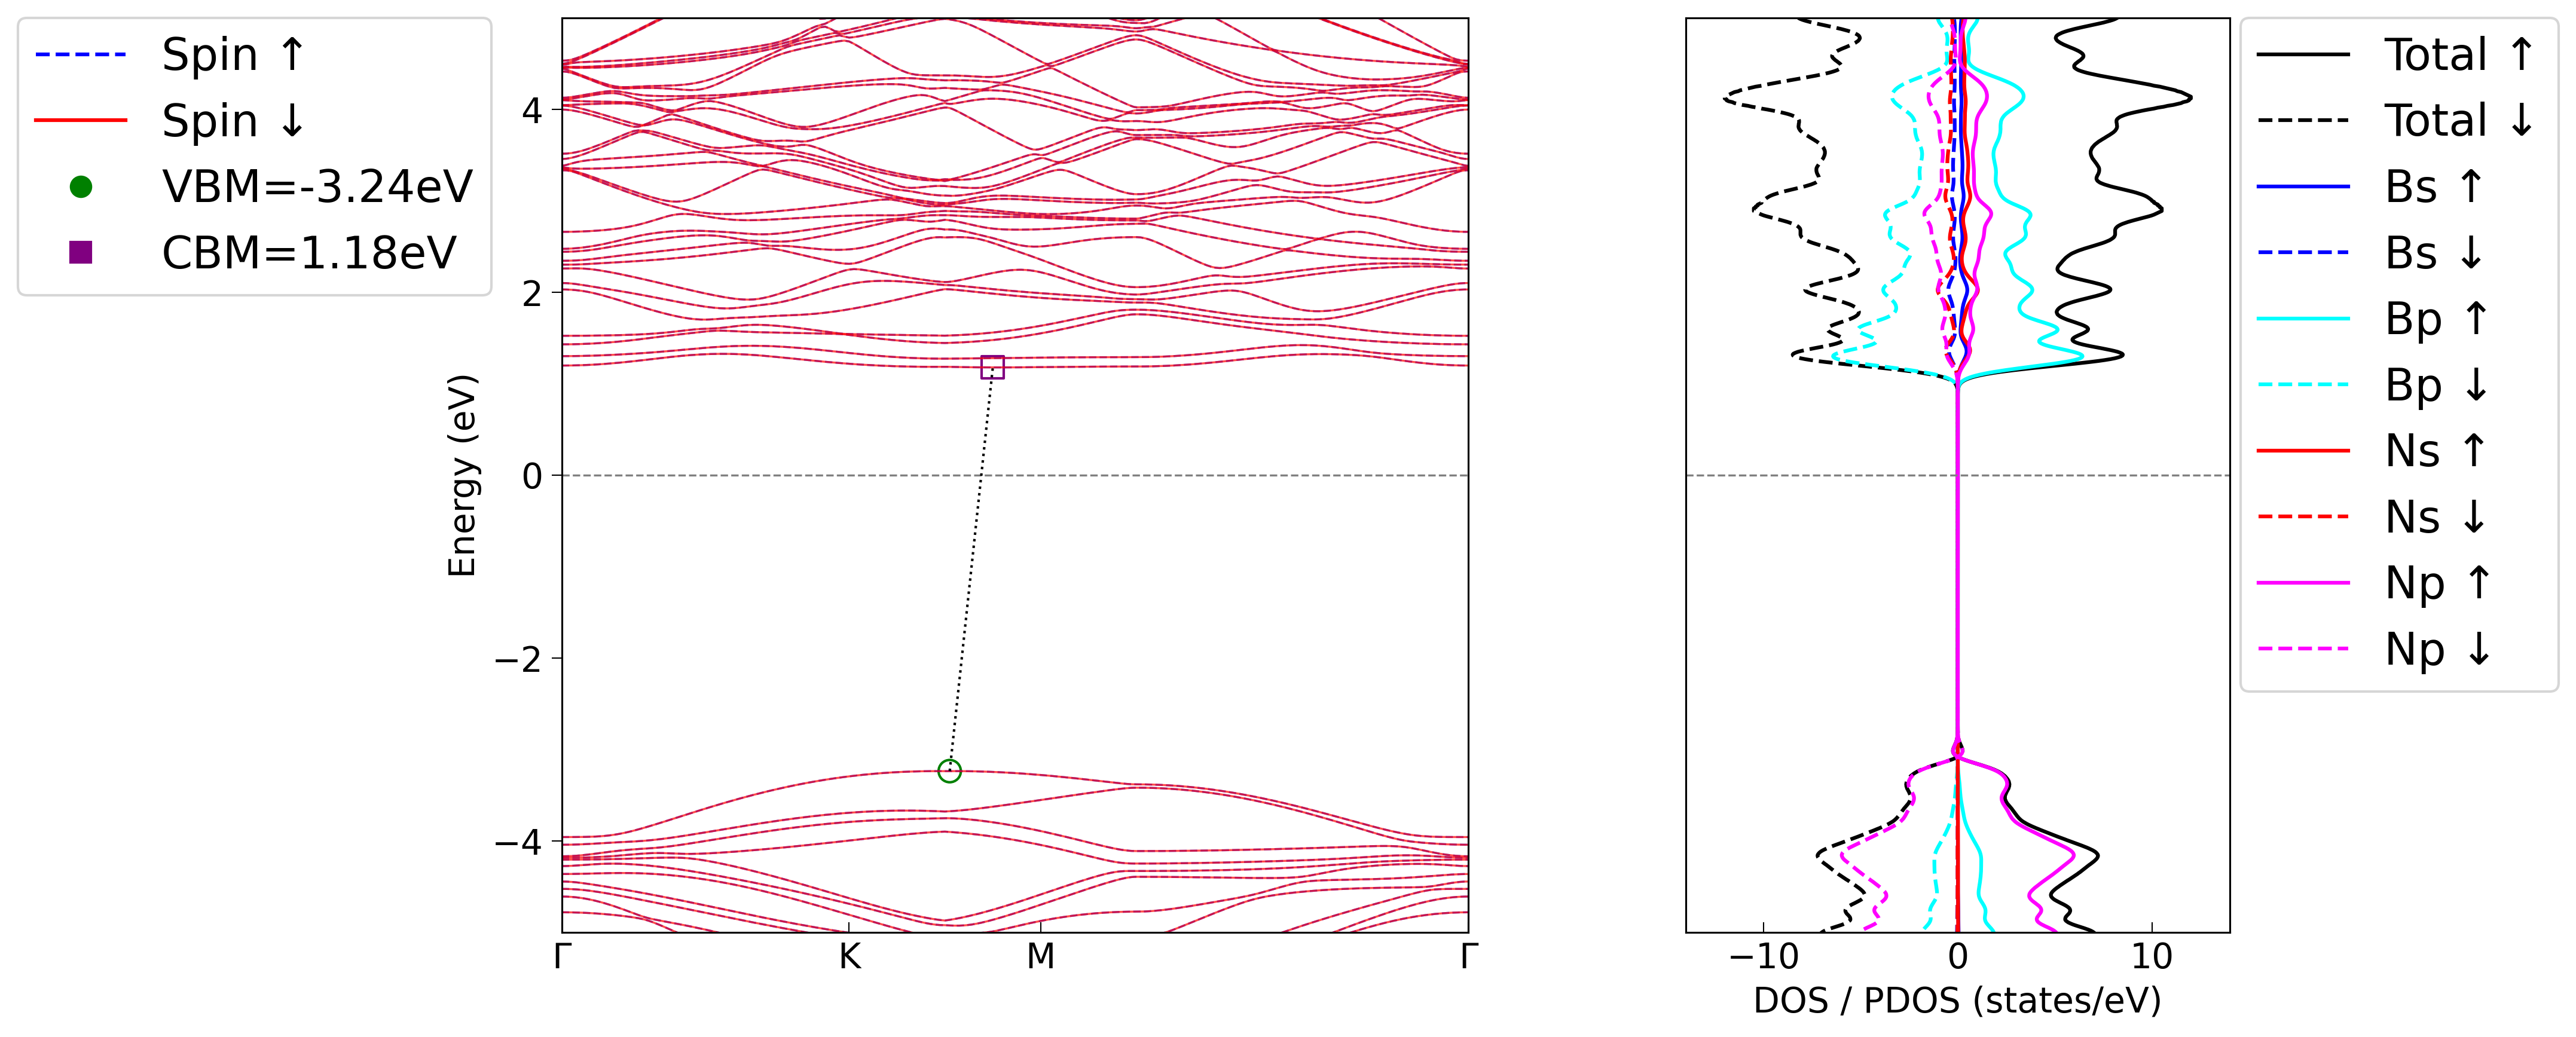
\includegraphics[width=0.95\textwidth]{gambar_hasil/simple_bands_pdos_pure_800K.png}
    \caption{Struktur pita elektronik dan PDOS untuk monolayer hBN murni pada 800 K. Celah pita menyempit menjadi $4.415$ eV.}
    \label{fig:hbn_pure_800K}
\end{figure}

\begin{figure}[htbp!] % PERUBAHAN: Ukuran gambar diperbesar
    \centering
    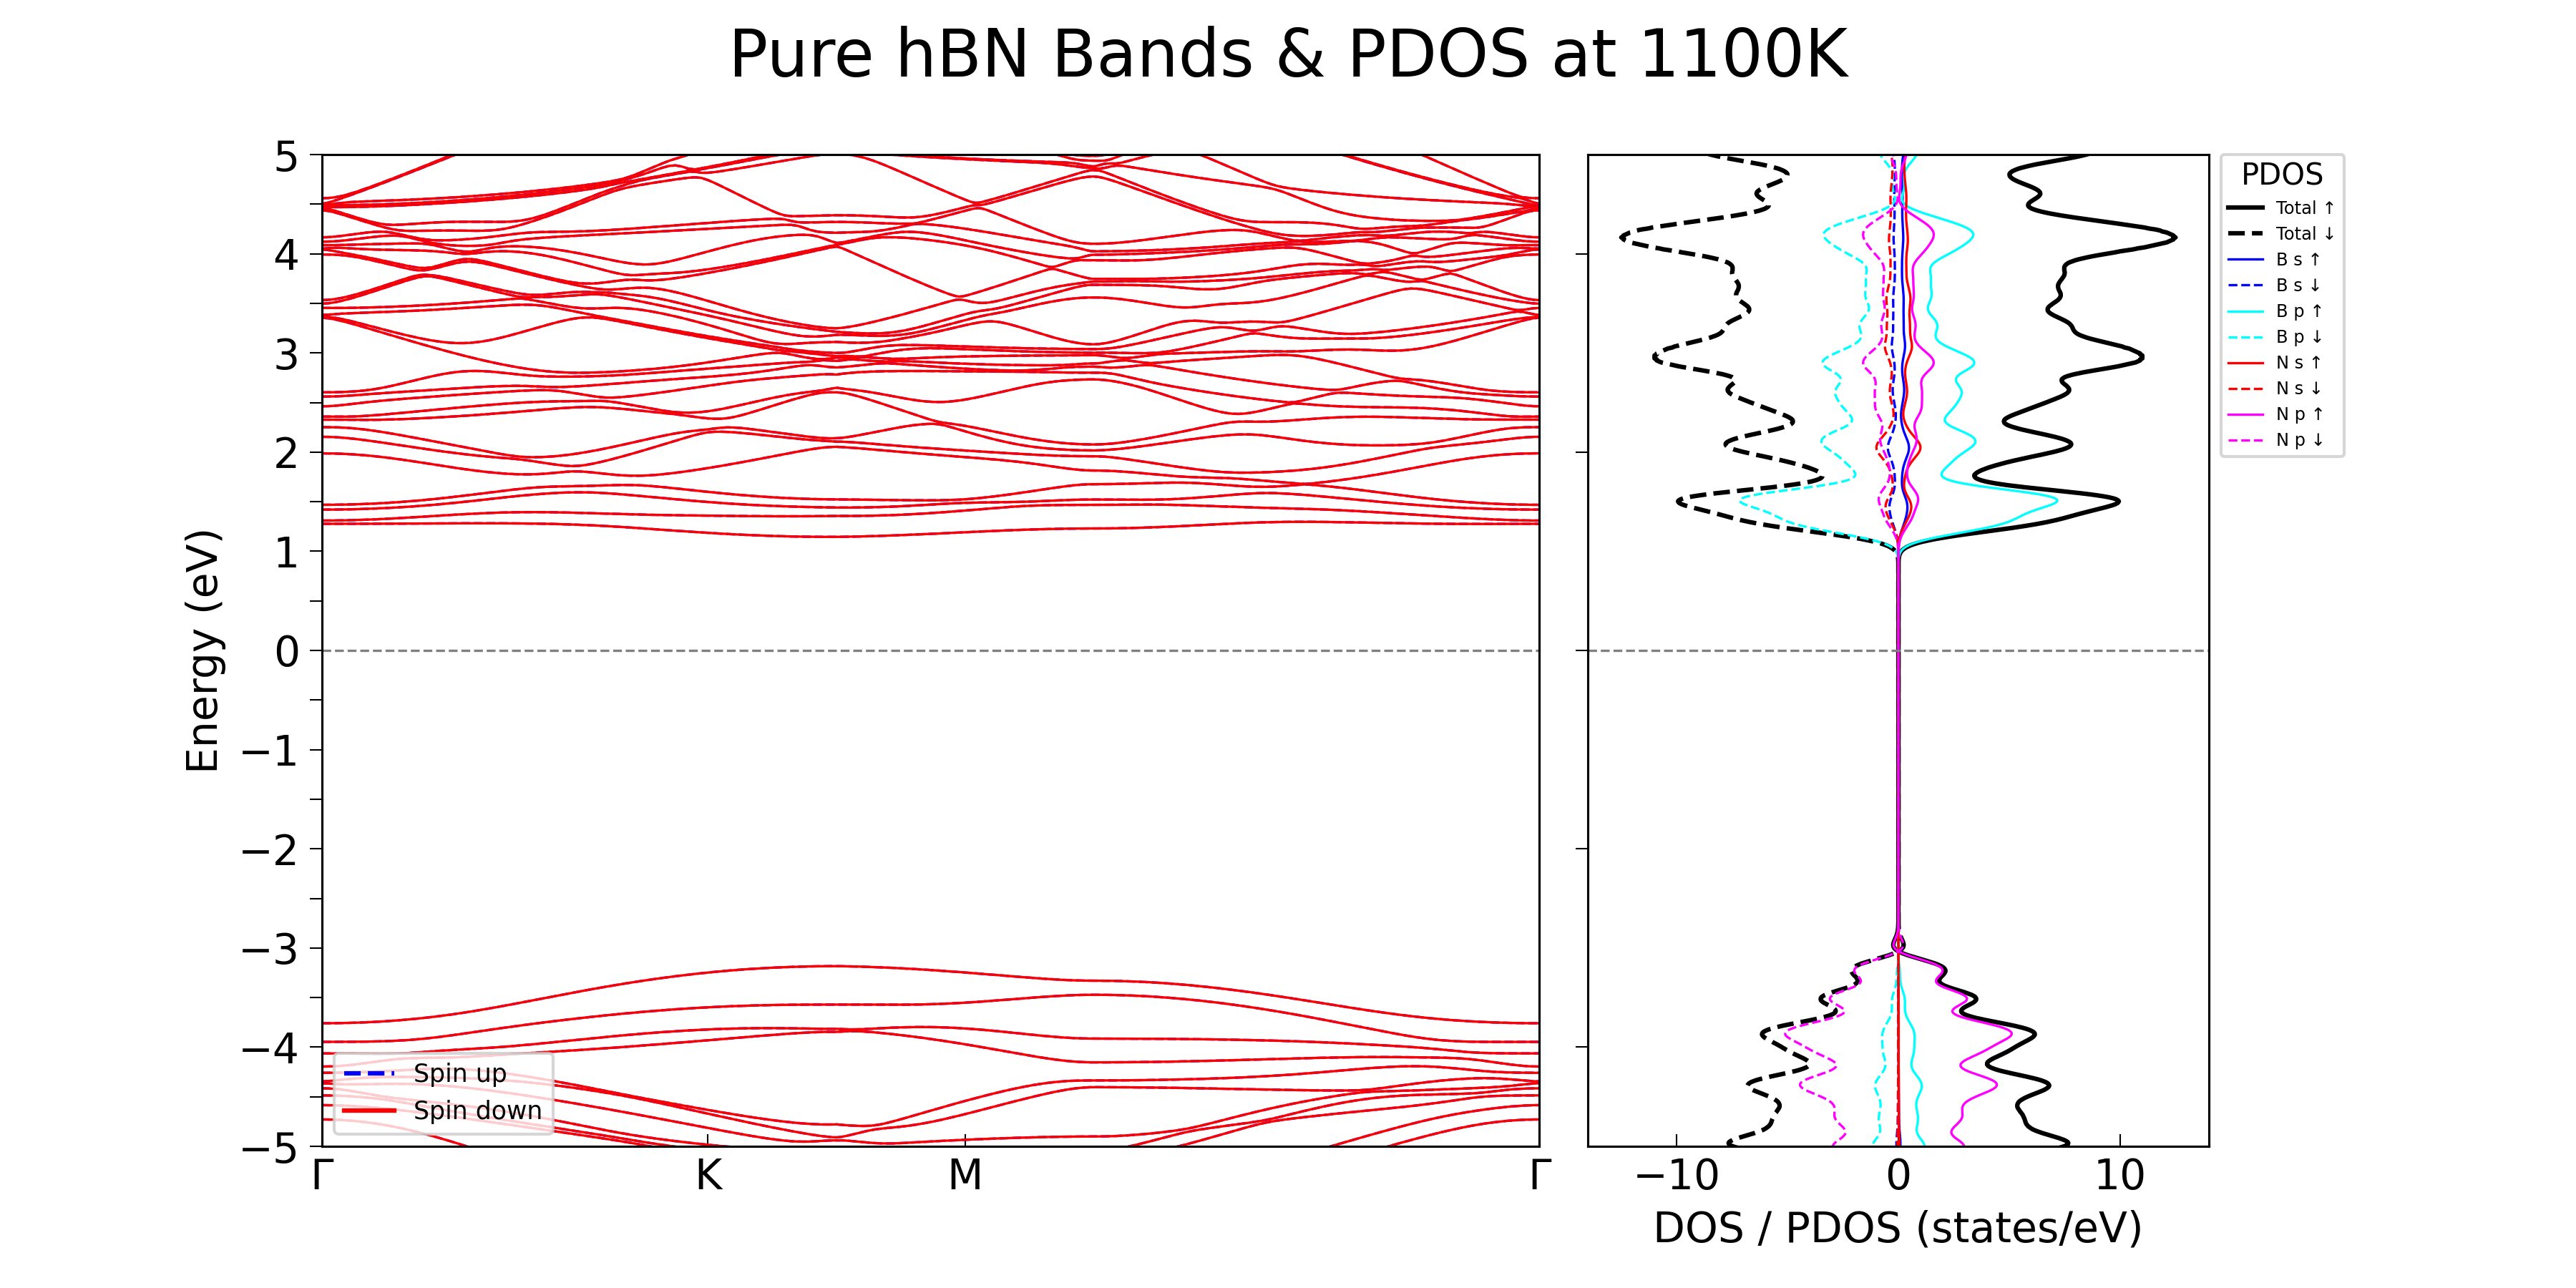
\includegraphics[width=0.95\textwidth]{gambar_hasil/simple_bands_pdos_pure_1100K.png}
    \caption{Struktur pita elektronik dan PDOS untuk monolayer hBN murni pada 1100 K. Celah pita menyempit lebih lanjut menjadi $4.328$ eV.}
    \label{fig:hbn_pure_1100K}
\end{figure}

\begin{figure}[htbp!] % PERUBAHAN: Ukuran gambar diperbesar
    \centering
    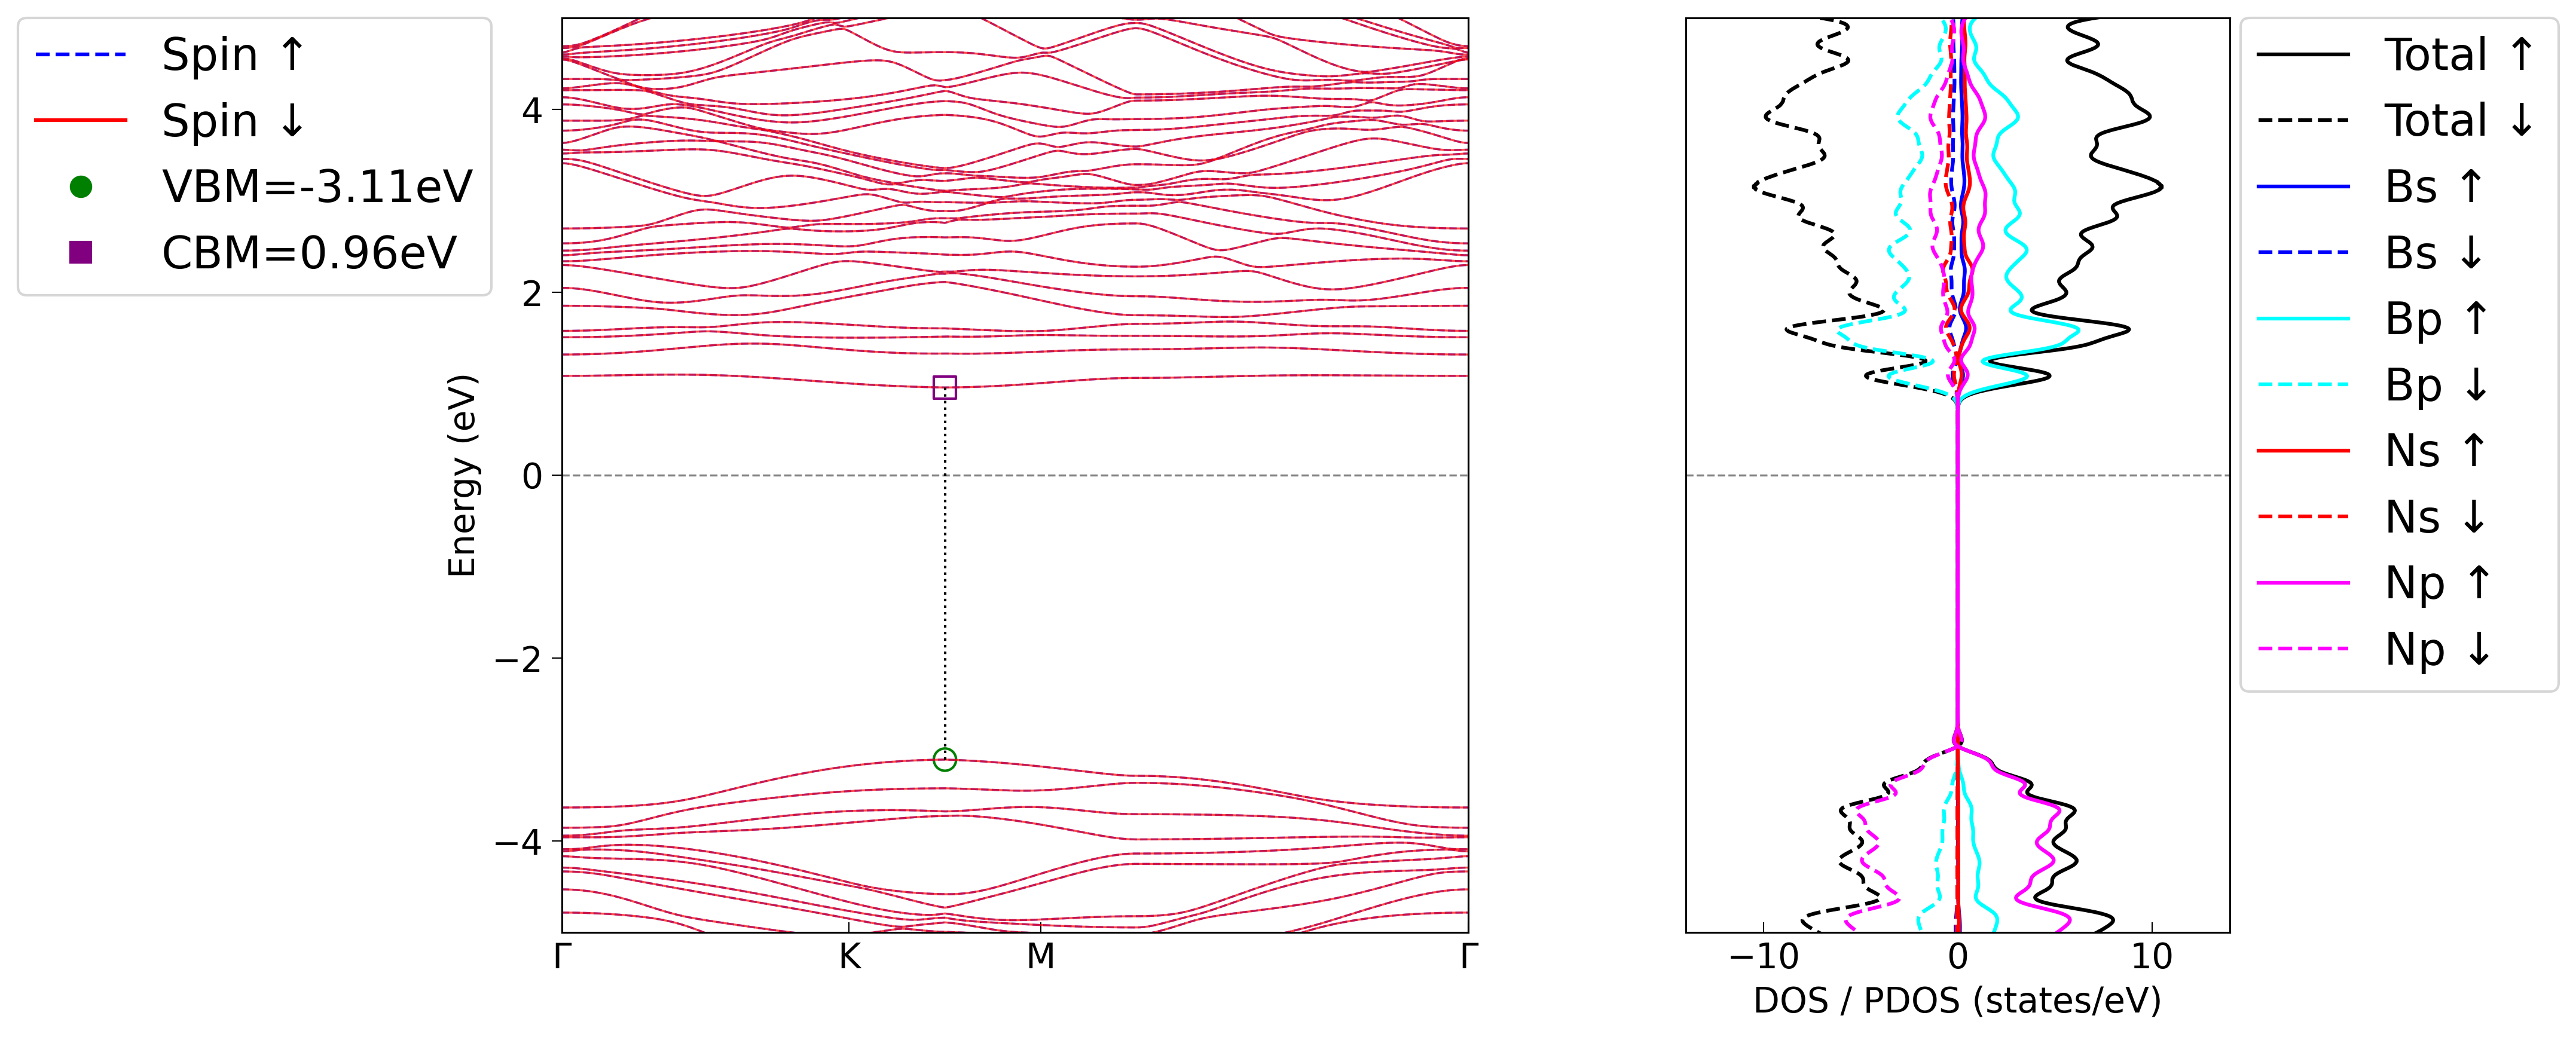
\includegraphics[width=0.95\textwidth]{gambar_hasil/simple_bands_pdos_pure_1225K.png}
    \caption{Struktur pita elektronik dan PDOS untuk monolayer hBN murni pada 1225 K. Celah pita menunjukkan penyempitan signifikan menjadi $4.069$ eV.}
    \label{fig:hbn_pure_1225K}
\end{figure}

Fenomena \emph{redshift} ini adalah manifestasi langsung dari kopling elektron-fonon (EPC).
Pada temperatur hingga, kisi tidak lagi statis; atom-atomnya bervibrasi di sekitar posisi kesetimbangannya. Kuantisasi dari vibrasi kisi ini disebut fonon.
Struktur atomik yang digunakan dalam kalkulasi DFT ini adalah "foto" sesaat atau \emph{snapshot} dari konfigurasi atom yang terdistorsi oleh fonon-fonon ini (pendekatan \emph{frozen-phonon}).
Ketika elektron bergerak melalui kisi yang bergetar ini, energinya direnormalisasi (diubah).
Menurut teori Allen-Heine-Cardona, ada dua kontribusi utama untuk perubahan ini \citep{Allen1983}: (1) koreksi energi-diri Fan-Migdal, di mana elektron "berpakaian" awan fonon virtual, dan (2) kontribusi Debye-Waller, di mana elektron bergerak dalam potensial periodik yang "tercoreng" oleh vibrasi termal.
Kedua efek ini hampir secara universal menyebabkan penurunan energi celah pita pada semikonduktor.
Dengan demikian, penurunan $E_g$ yang diamati dari Gambar \ref{fig:hbn_pure_800K} hingga \ref{fig:hbn_pure_1225K} adalah cerminan dari meningkatnya populasi fonon dan penguatan efek EPC pada temperatur yang lebih tinggi.
Hasil \emph{redshift} yang konsisten ini tampak kontras dengan beberapa laporan eksperimental pada hBN multilayer, yang menunjukkan pergeseran biru (\emph{blueshift}) anomali pada temperatur tinggi \citep{Du2017}.
\emph{Blueshift} tersebut diatribusikan pada dominasi efek Ekspansi Termal Negatif (NTE), di mana kontraksi kisi akibat moda fonon lentur memperlebar celah pita.
Seperti yang telah dibahas pada Bagian \ref{subsec:md_reaxff}, potensial ReaxFF yang digunakan kemungkinan besar tidak menangkap mekanisme NTE ini.
Akibatnya, simulasi ini secara efektif mengisolasi kontribusi dari EPC. Oleh karena itu, \emph{redshift} yang diamati bukanlah sebuah kontradiksi, melainkan hasil yang konsisten secara internal dengan fisika yang "diizinkan" oleh model: tanpa adanya mekanisme \emph{blueshift} dari NTE, mekanisme \emph{redshift} dari EPC menjadi dominan dan secara akurat ditangkap oleh kalkulasi DFT.

\subsection{Analisis Visual Kerapatan Muatan dan Spin}
\label{subsec:hbn_pure_density_analysis}
Untuk melengkapi analisis struktur pita, visualisasi distribusi elektron dalam ruang nyata memberikan wawasan kualitatif yang kuat.
Gambar \ref{fig:hbn_pure_density} menyajikan plot kerapatan muatan dan kerapatan spin untuk sistem hBN murni pada setiap temperatur.

%%%%%%%%%%%%%%%%%%%%%%%%%%%%%%%%%%%%%%%%%%%%%%%%%%%%%%%%%%%%%%%%%%%%%%
% PERBAIKAN GAMBAR: KERAPATAN MUATAN/SPIN (MURNI)
% Permintaan: Membuat gambar lebih besar.
% Solusi: Menggunakan lebar 0.49\textwidth untuk setiap subfigure memastikan
% gambar mengisi lebar teks secara horizontal, memberikan ukuran maksimal
% untuk tata letak dua kolom.
%%%%%%%%%%%%%%%%%%%%%%%%%%%%%%%%%%%%%%%%%%%%%%%%%%%%%%%%%%%%%%%%%%%%%%
\begin{figure}[htbp!]
  \centering
  \begin{subfigure}[b]{0.49\textwidth}
    \centering
    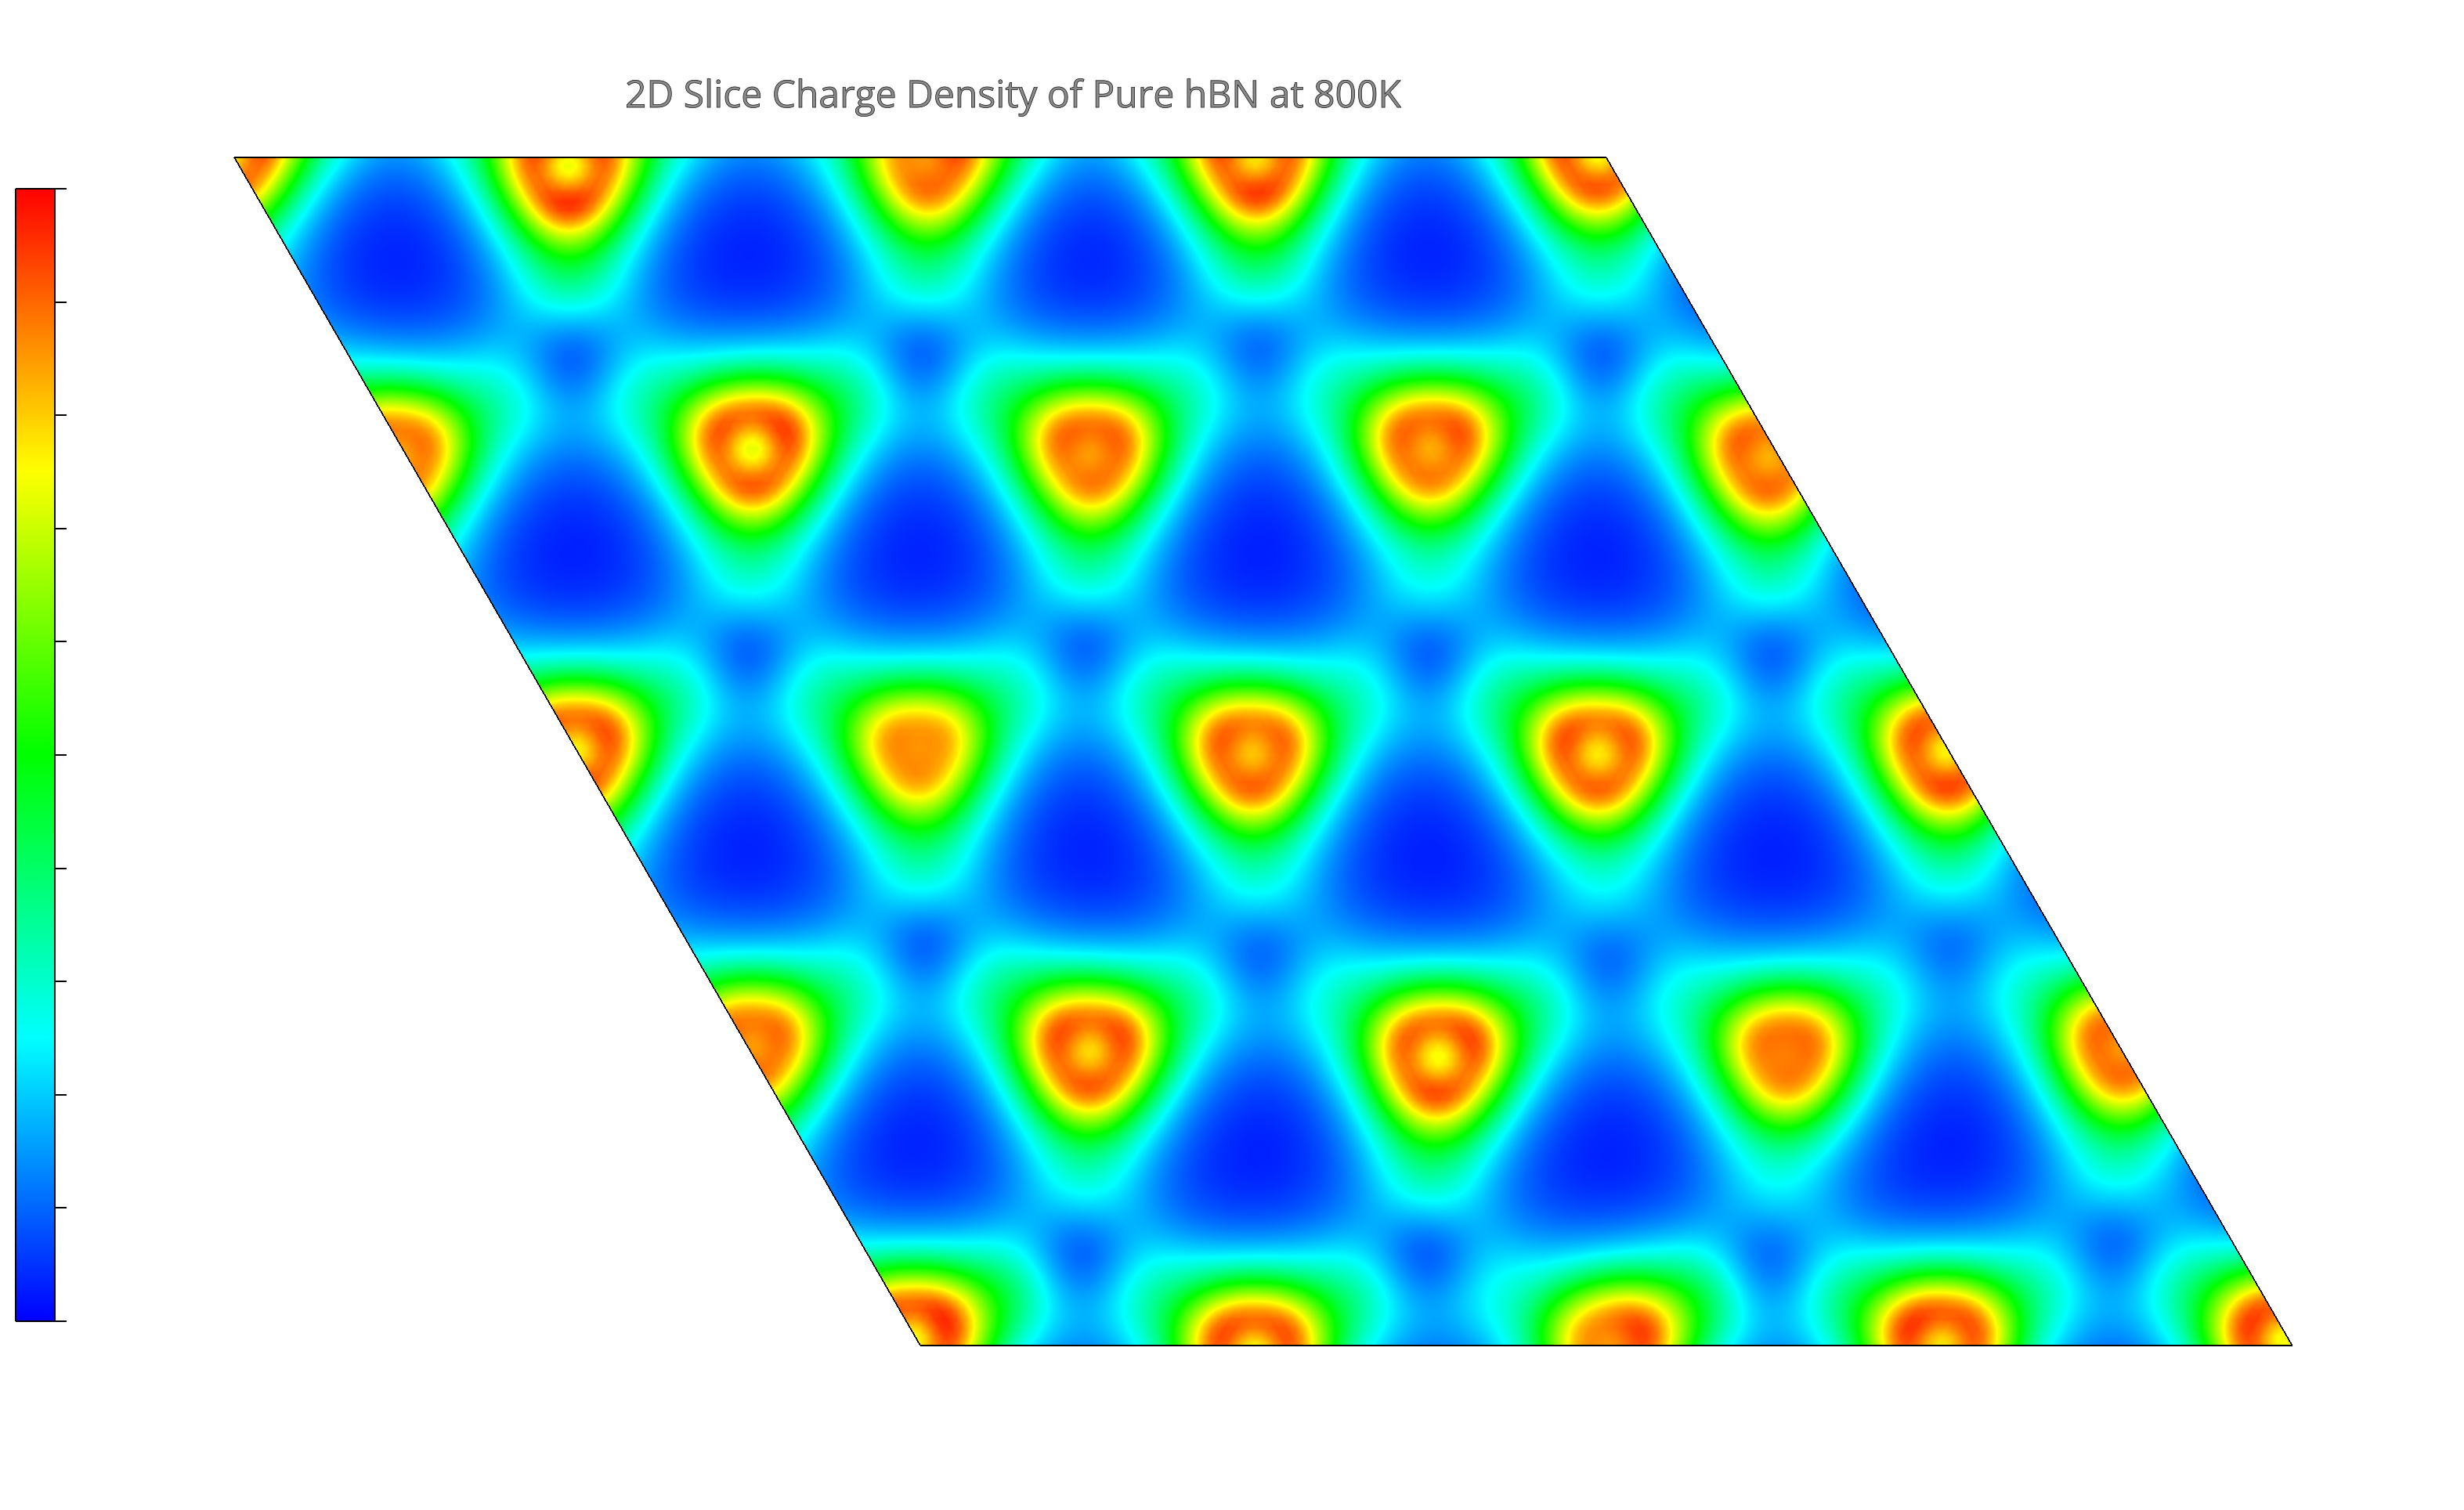
\includegraphics[width=\linewidth]{hBN_rho_pure_800K.png}
    \caption{Kerapatan Muatan, 800 K}
    \label{subfig:rho_pure_800k}
  \end{subfigure}\hfill
  \begin{subfigure}[b]{0.49\textwidth}
    \centering
    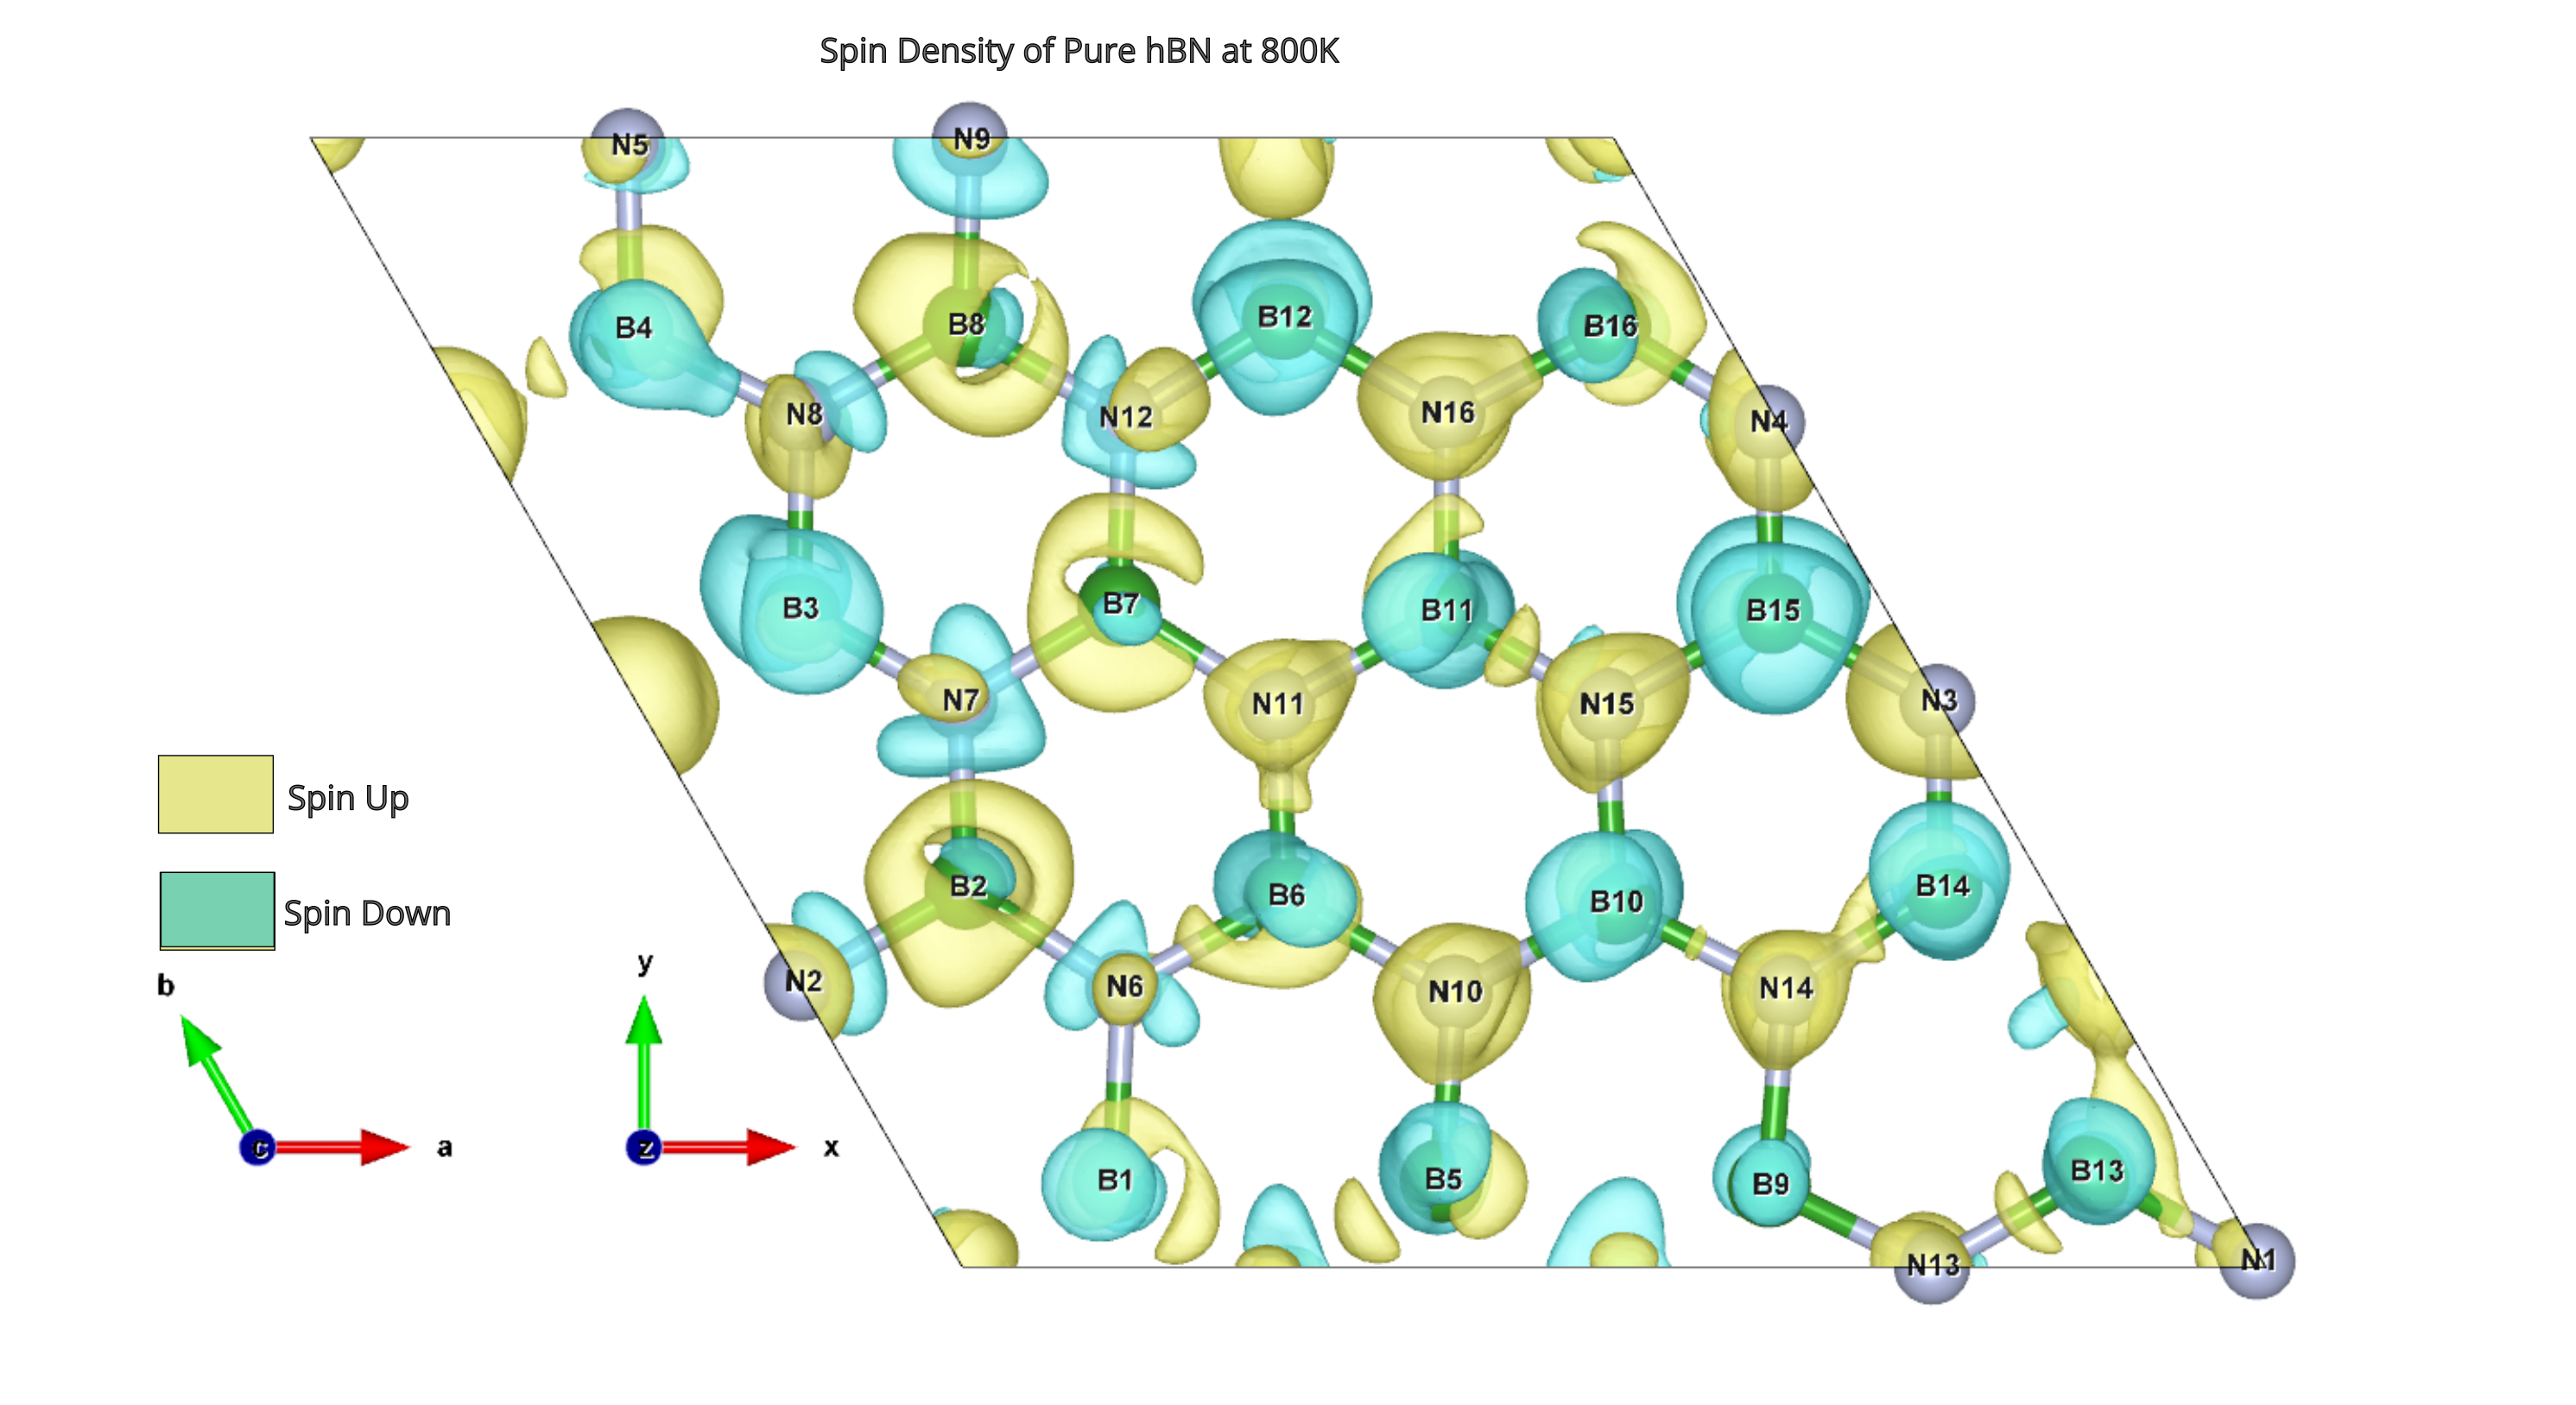
\includegraphics[width=\linewidth]{hBN_spin_pure_800K.png}
    \caption{Kerapatan Spin, 800 K}
    \label{subfig:spin_pure_800k}
  \end{subfigure}
  \vspace{1em}

  \begin{subfigure}[b]{0.49\textwidth}
    \centering
    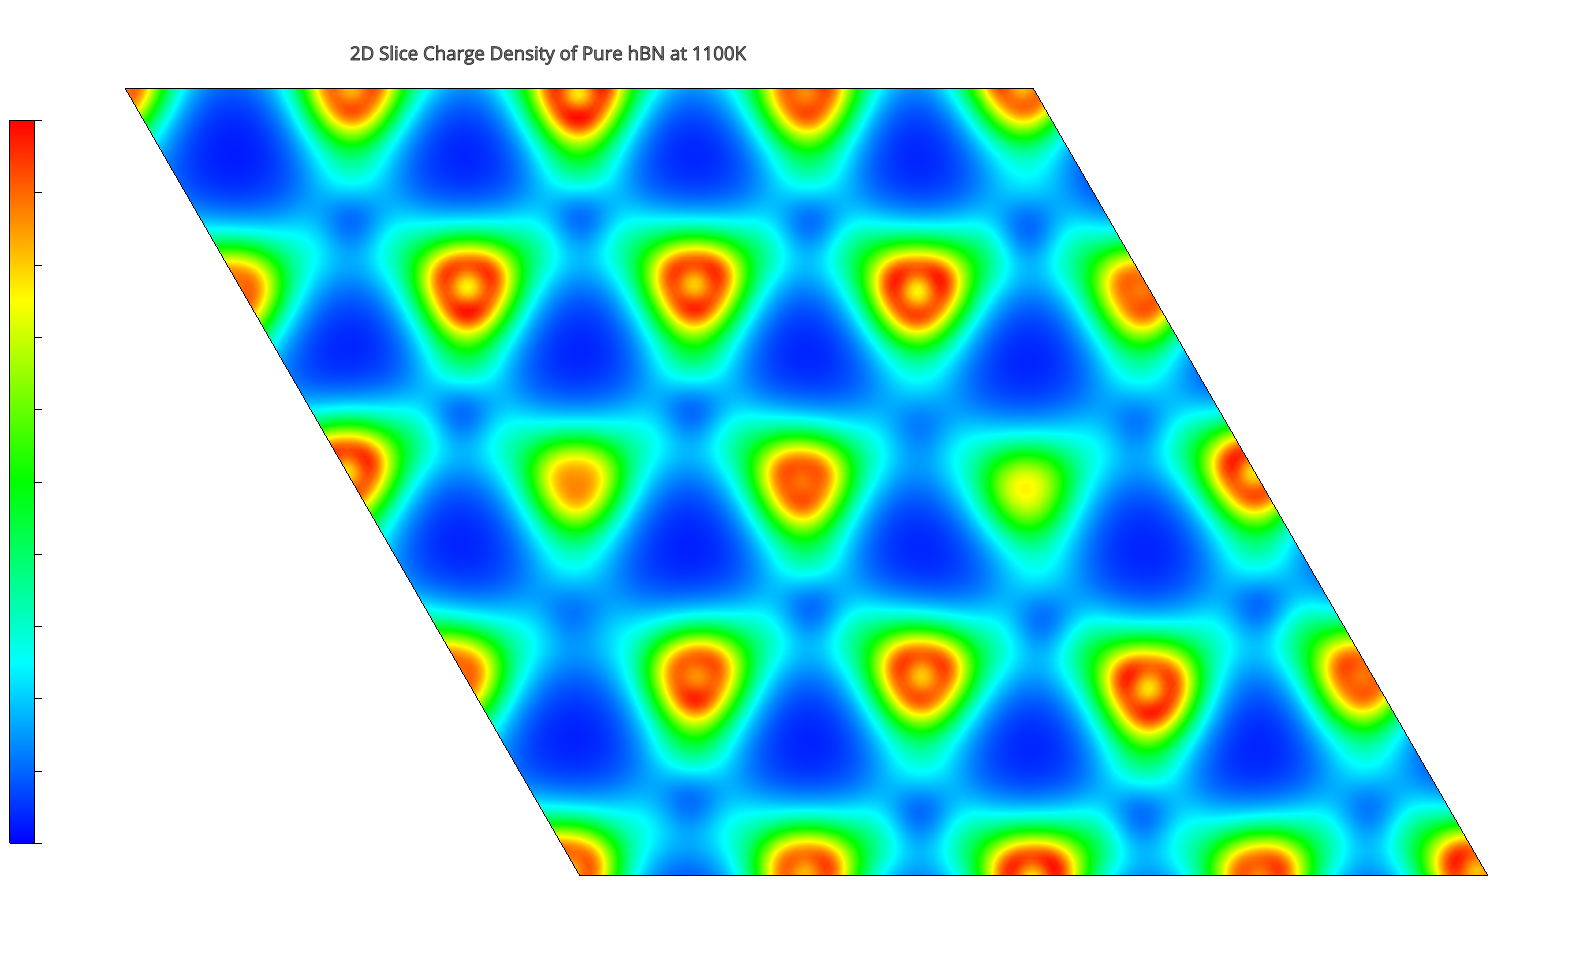
\includegraphics[width=\linewidth]{hBN_rho_pure_1100K.png}
    \caption{Kerapatan Muatan, 1100 K}
    \label{subfig:rho_pure_1100k}
  \end{subfigure}\hfill
  \begin{subfigure}[b]{0.49\textwidth}
    \centering
    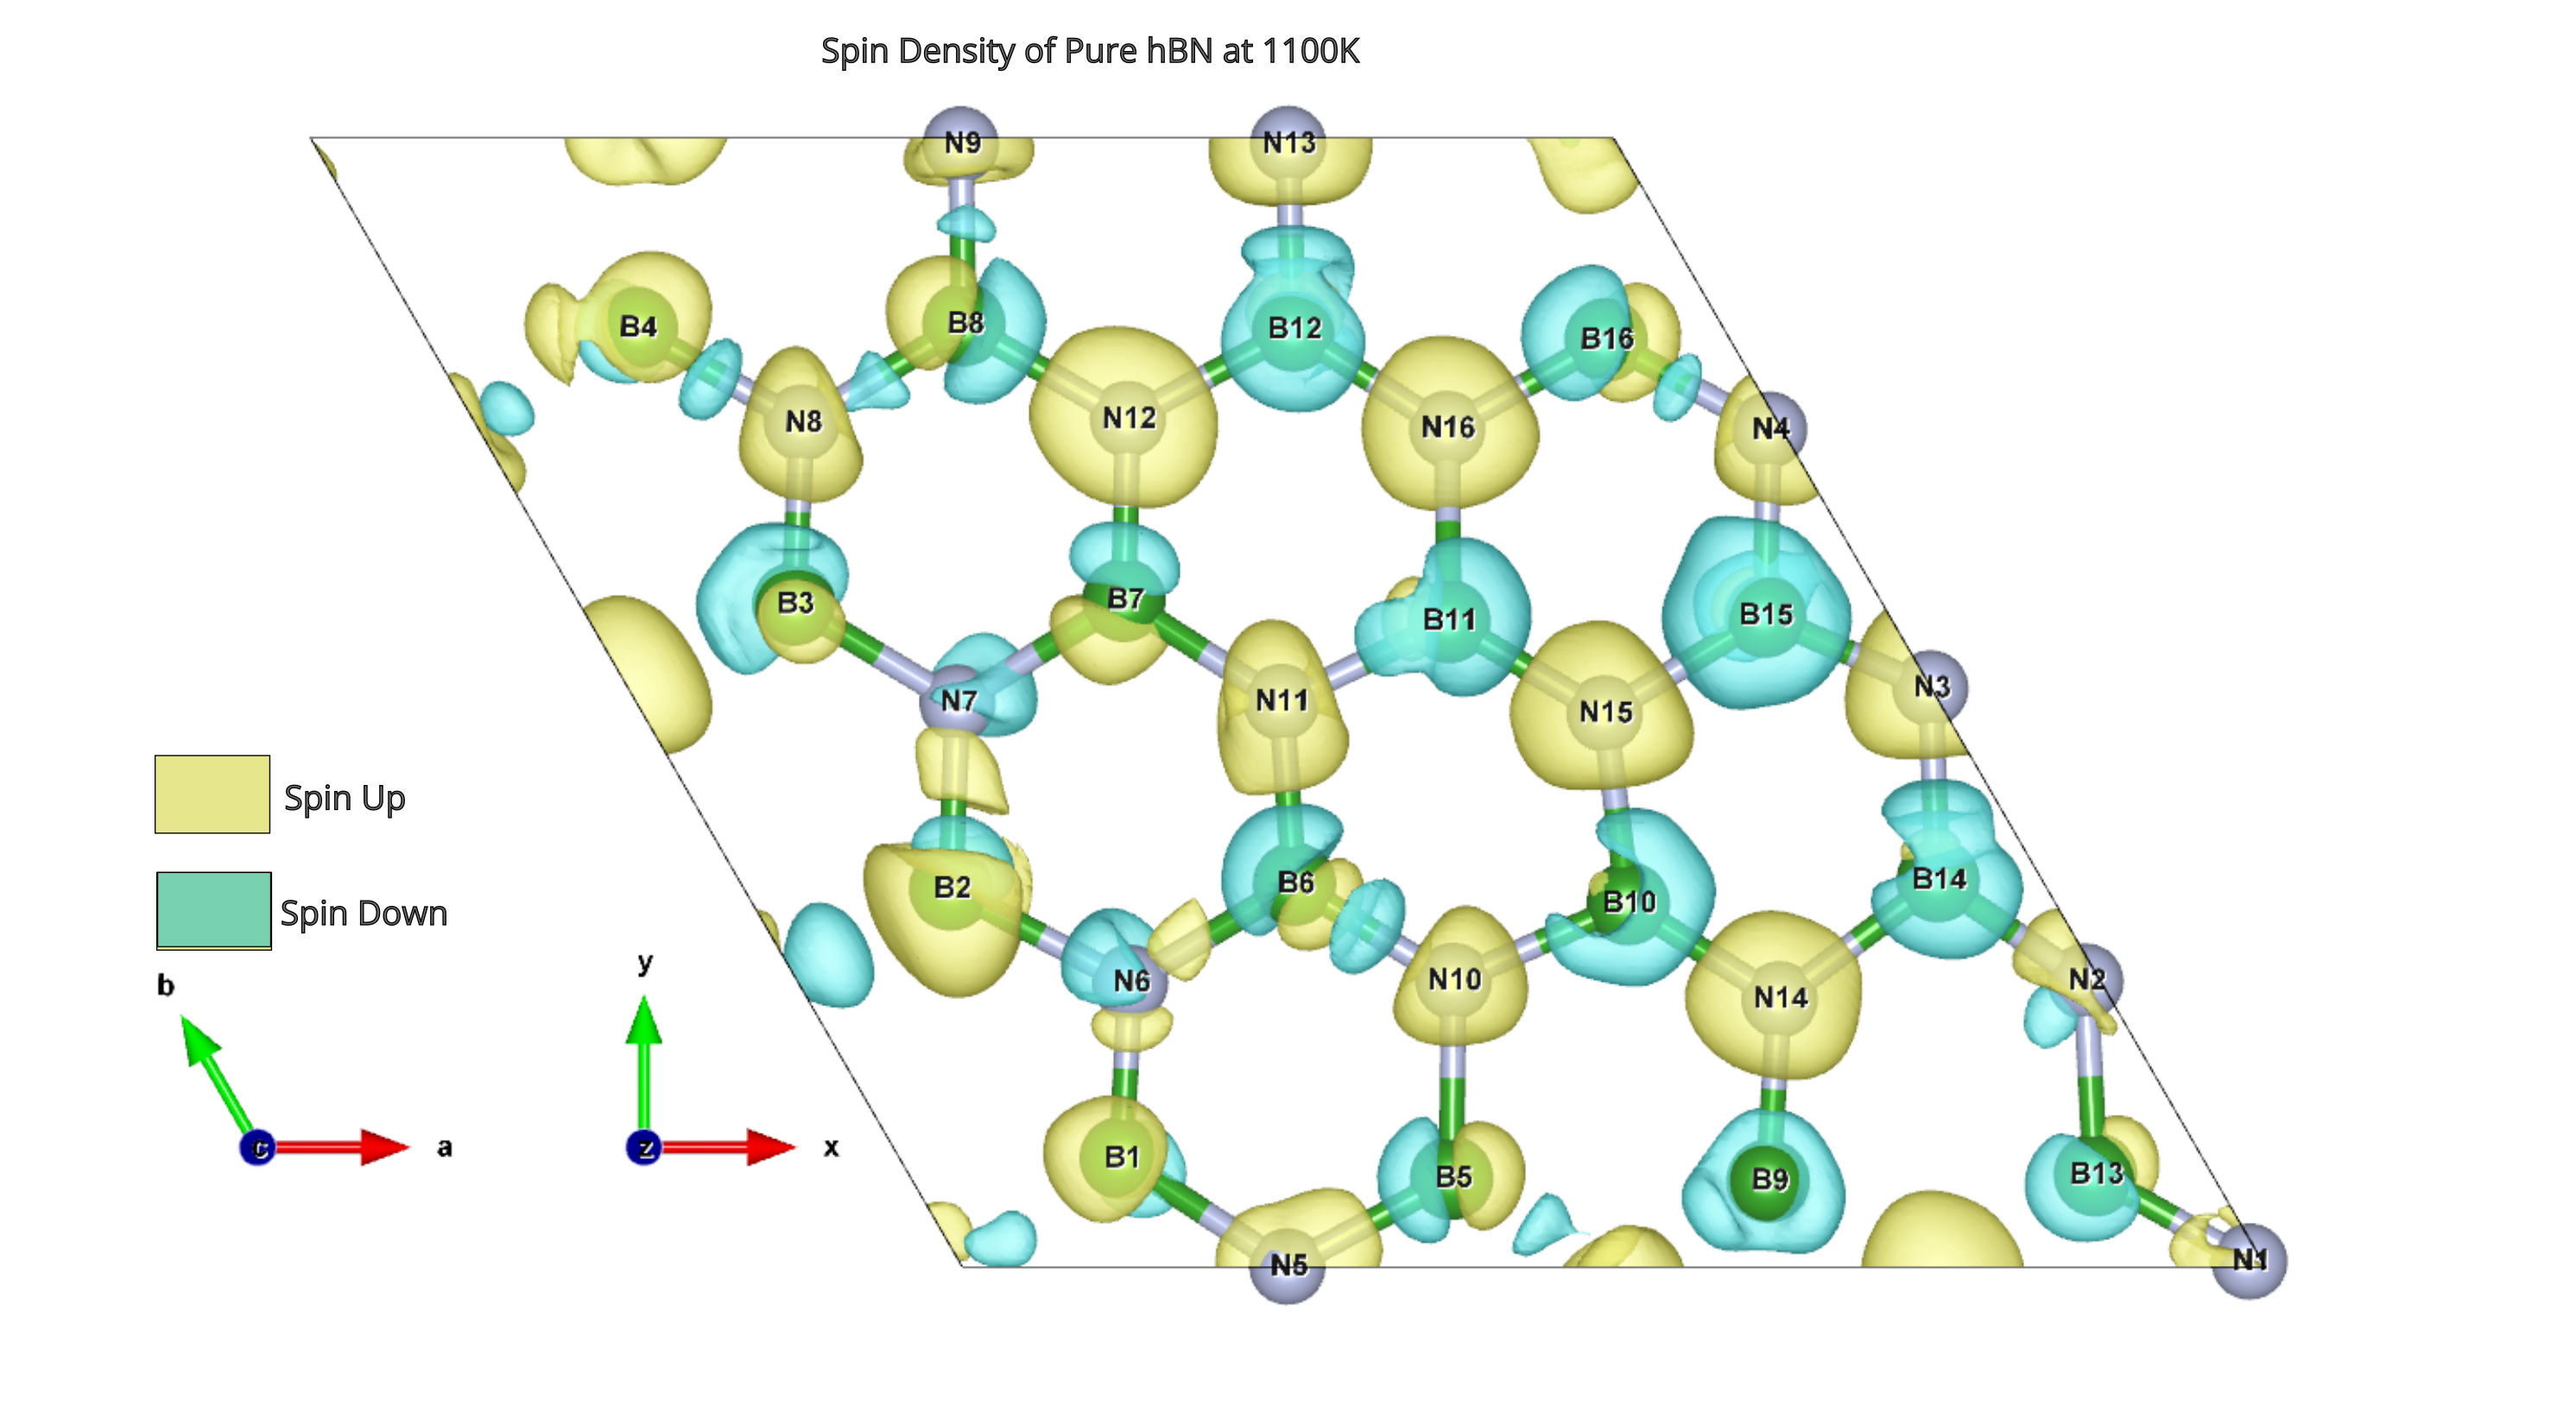
\includegraphics[width=\linewidth]{hBN_spin_pure_1100K.png}
    \caption{Kerapatan Spin, 1100 K}
    \label{subfig:spin_pure_1100k}
  \end{subfigure}
  \vspace{1em}

  \begin{subfigure}[b]{0.49\textwidth}
    \centering
    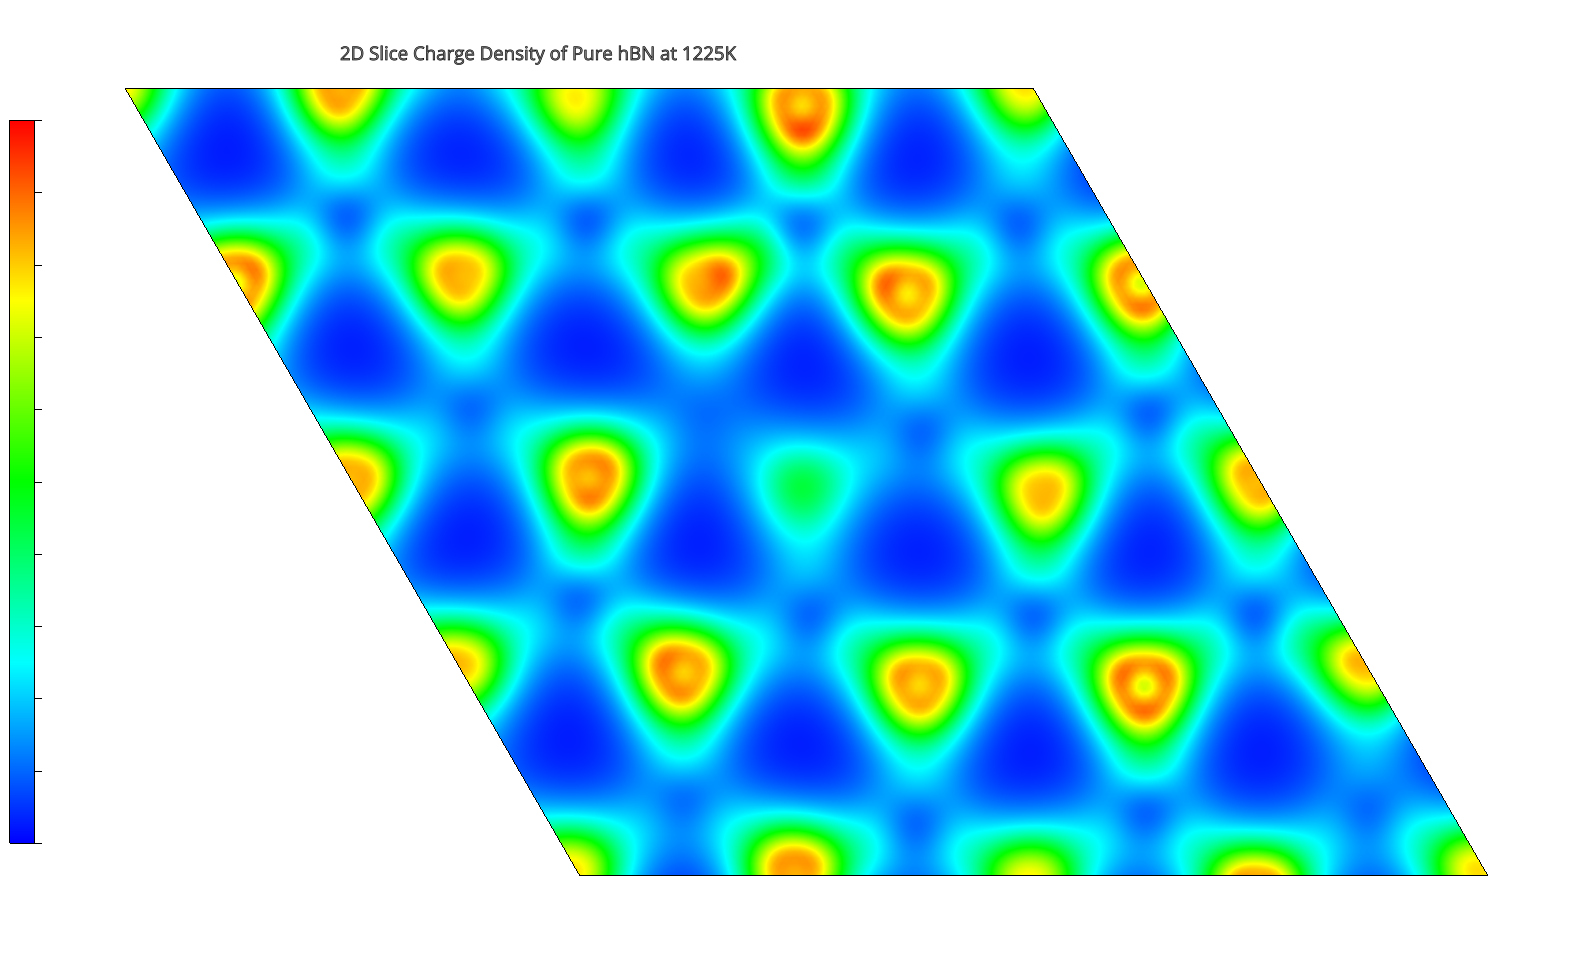
\includegraphics[width=\linewidth]{hBN_rho_pure_1225K.png}
    \caption{Kerapatan Muatan, 1225 K}
    \label{subfig:rho_pure_1225k}
  \end{subfigure}\hfill
  \begin{subfigure}[b]{0.49\textwidth}
    \centering
    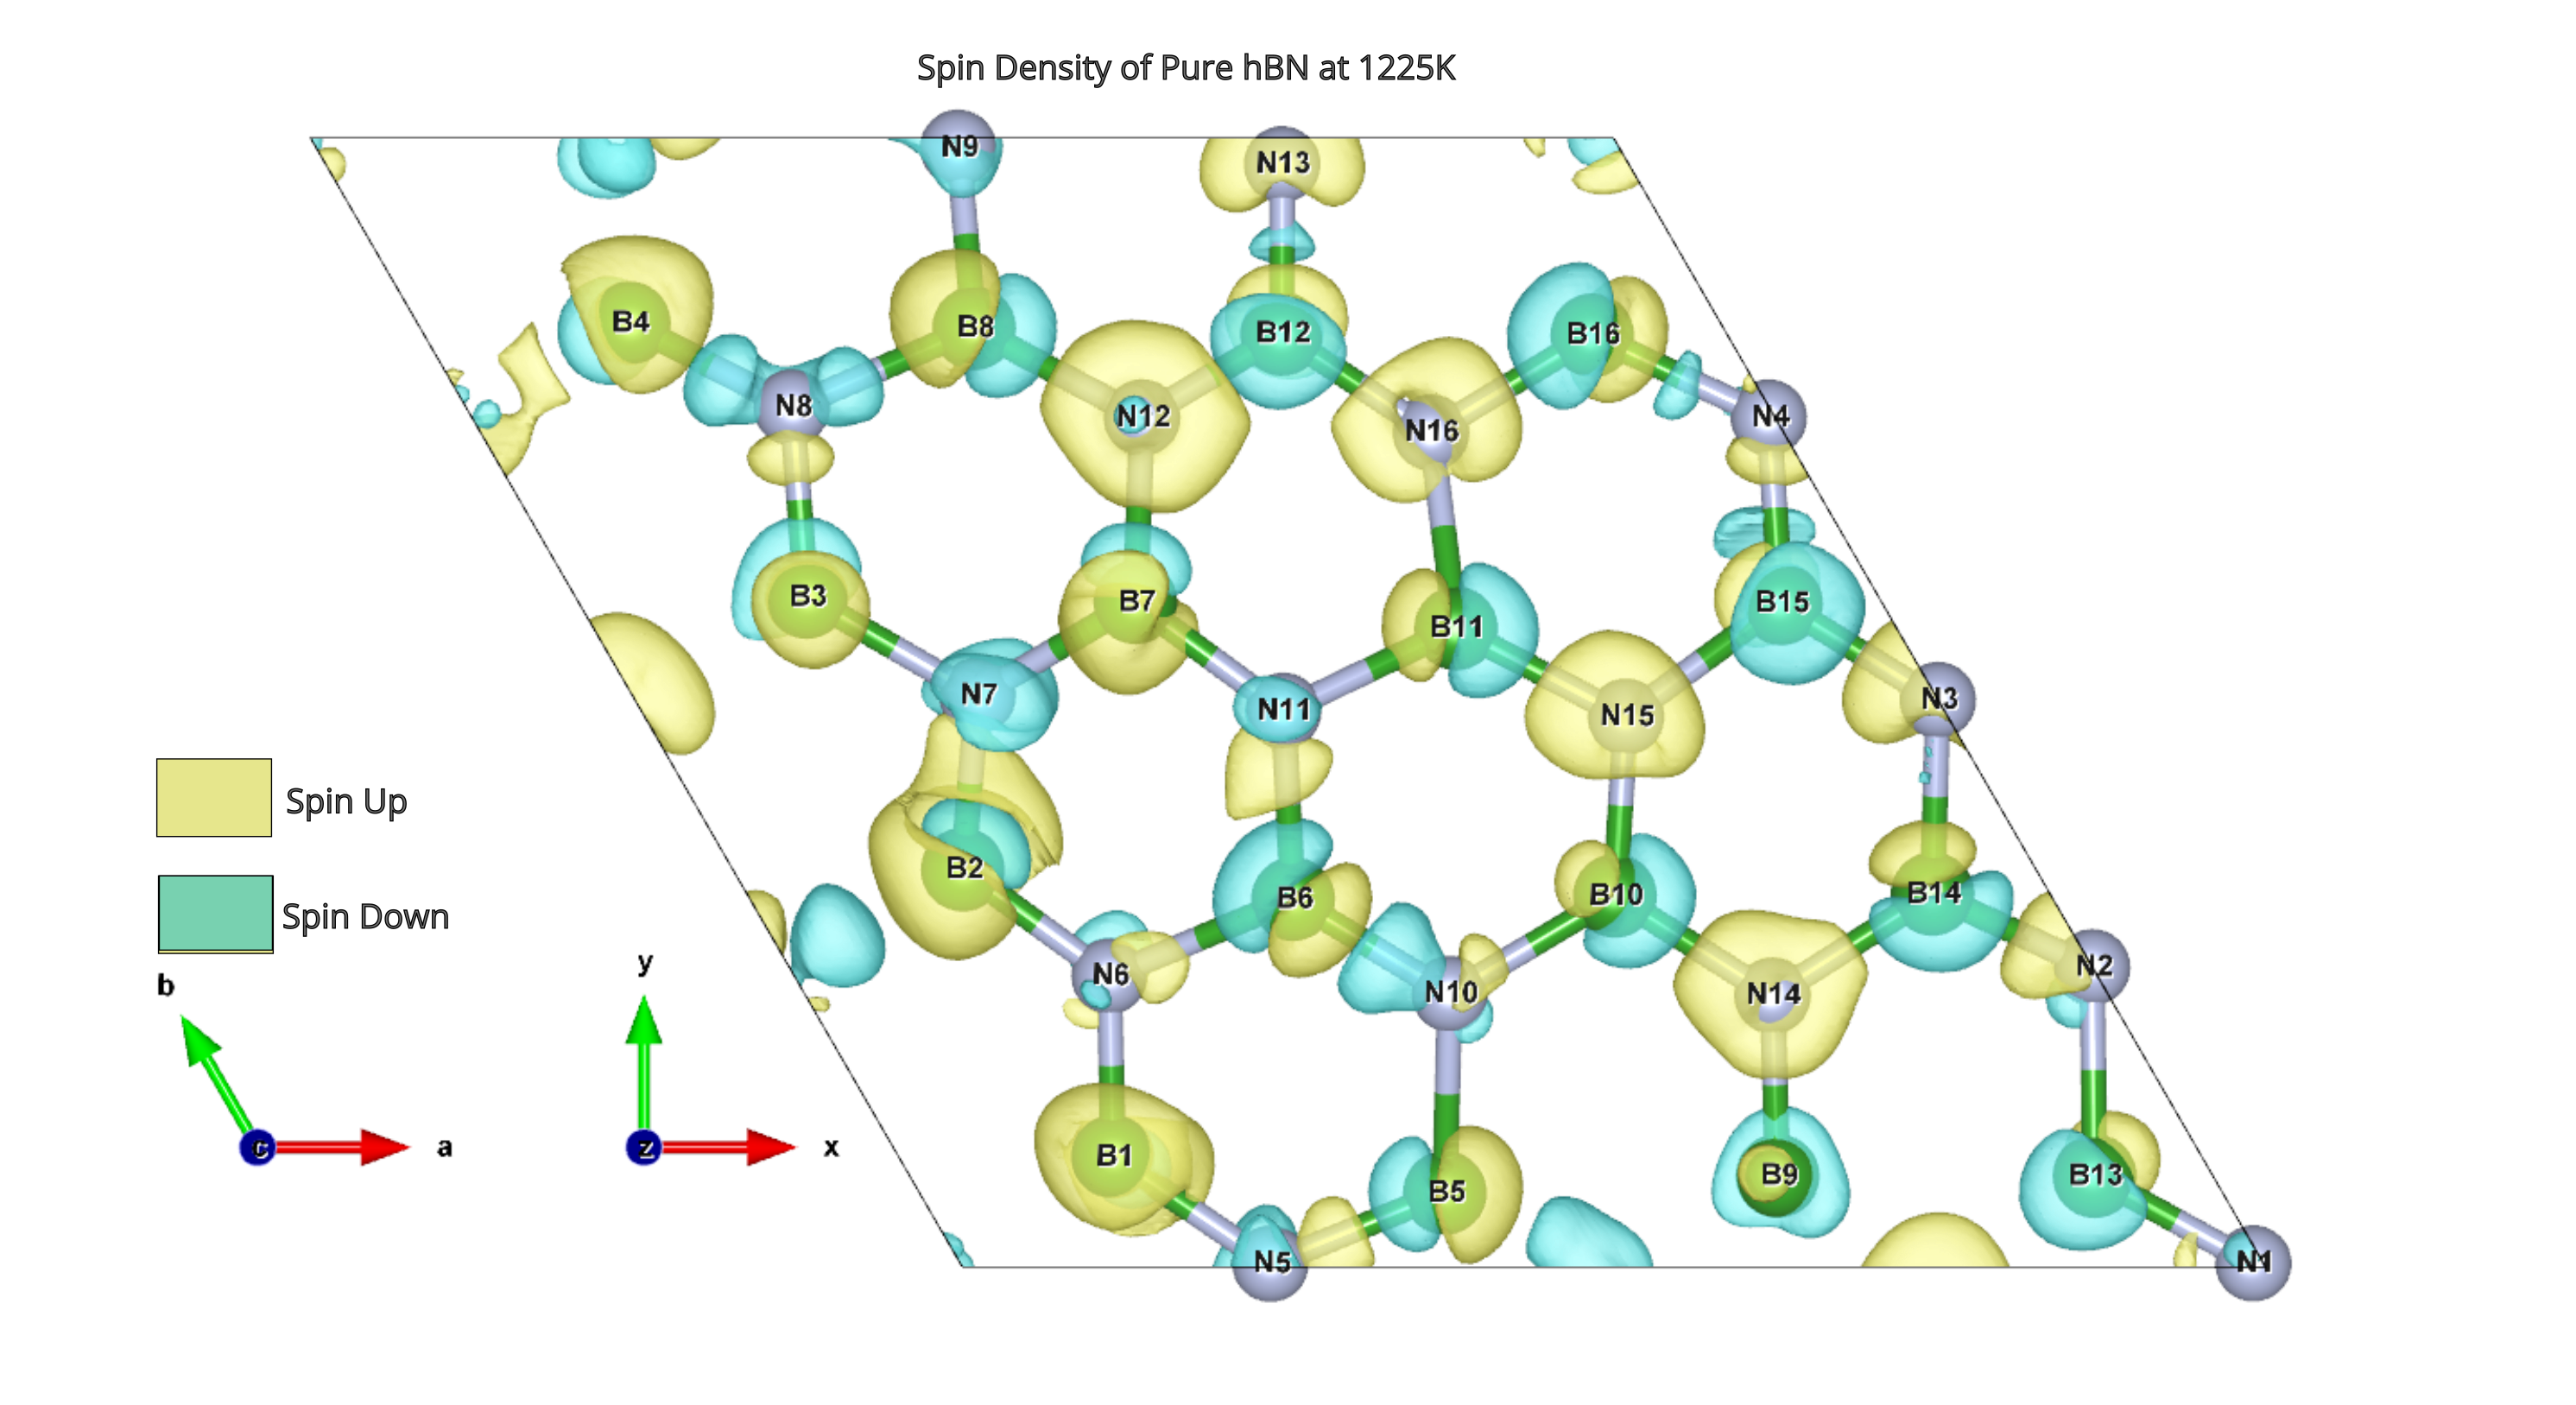
\includegraphics[width=\linewidth]{hBN_spin_pure_1225K.png}
    \caption{Kerapatan Spin, 1225 K}
    \label{subfig:spin_pure_1225k}
  \end{subfigure}

  \caption{Visualisasi 2D dari kerapatan muatan total (kiri) dan kerapatan spin (kanan) untuk monolayer hBN murni pada 800 K, 1100 K, dan 1225 K. Warna merah pada kerapatan muatan menunjukkan akumulasi elektron, sedangkan warna biru menunjukkan deplesi. Untuk kerapatan spin, warna biru menunjukkan spin down dan warna kuning menunjukan spin up.}
  \label{fig:hbn_pure_density}
\end{figure}

Plot kerapatan muatan (Gambar \ref{fig:hbn_pure_density}a, c, e) secara konsisten menunjukkan akumulasi kerapatan elektron yang signifikan di sekitar situs atom nitrogen (merah) dan deplesi di sekitar situs atom boron (biru).
Ini adalah bukti visual langsung dari sifat ikatan kovalen polar yang kuat dalam hBN, yang timbul dari perbedaan elektronegativitas yang besar antara B dan N. Meskipun struktur atomik mengalami distorsi termal dan \emph{rippling} (seperti yang ditunjukkan pada Gambar \ref{fig:md_structures_per_condition}), distribusi muatan dalam bidang ini tetap sangat teratur dan periodik.
Hal ini mencerminkan ketahanan kerangka ikatan $\sigma$ yang kuat, yang mendefinisikan sifat elektronik dasar material.
Yang tidak kalah penting adalah analisis kerapatan spin (Gambar \ref{fig:hbn_pure_density}b, d, f).
Untuk semua temperatur yang diselidiki, plot menunjukkan nilai nol yang seragam di seluruh supercell.
Ini adalah konfirmasi visual yang definitif bahwa hBN murni adalah material non-magnetik.
Tidak adanya polarisasi spin (perbedaan antara kerapatan elektron spin-atas dan spin-bawah) secara sempurna sejalan dengan struktur pita yang simetris untuk kedua kanal spin (misalnya, Gambar \ref{fig:hbn_pure_1225K}) dan nilai magnetisasi total nol yang dilaporkan dalam Tabel \ref{tab:hbn_murni_suhu}.
Hasil ini menegaskan bahwa agitasi termal, meskipun cukup untuk menyebabkan distorsi kisi yang signifikan dan merenormalisasi celah pita, tidak cukup untuk memecah simetri spin dan menginduksi momen magnetik.
Pengamatan ini menetapkan dasar referensi yang krusial untuk mengevaluasi dampak pengenalan cacat.

\section{Rekayasa Sifat Elektronik dan Magnetik Melalui Cacat Antisite}
\label{sec:hbn_defek}
Kehadiran cacat titik secara fundamental mengubah lanskap elektronik material, seringkali mengintroduksi perilaku yang tidak ada pada material induknya.
Bagian ini membahas bagaimana dua jenis cacat antisite, N\textsubscript{B} (Nitrogen pada situs Boron) dan B\textsubscript{N} (Boron pada situs Nitrogen), secara dramatis memodulasi sifat elektronik dan magnetik monolayer hBN sebagai respons terhadap temperatur.
\subsection{Cacat N\textsubscript{B}: Pergeseran Biru Anomali dan Kopling Elektron-Fonon Terlokalisasi}
\label{subsec:hbn_defek_nb}
Introduksi cacat antisite N\textsubscript{B} menyebabkan perubahan drastis pada struktur elektronik.
Seperti yang ditunjukkan pada Gambar \ref{fig:hbn_NN_800K}, cacat ini menciptakan tingkat-tingkat energi baru yang terlokalisasi di dalam celah pita intrinsik hBN, secara signifikan mengurangi celah pita efektif menjadi $0.694$ eV pada 800 K.
\begin{table}[htbp!] % STANDARISASI: Menggunakan [htbp!]
  \centering
  \caption{Sifat Elektronik Monolayer hBN dengan Cacat Antisite N\textsubscript{B} sebagai Fungsi Temperatur.}
  \label{tab:hbn_defek_nb}
  \begin{tabular}{lcccccc}
    \toprule
    Temperatur & VBM & CBM & $E_g$ & $E_F$ & Magnetisasi & Magnetisasi \\
    (K) & (eV) & (eV) & (eV) & (eV) & Total ($\mu_B$) & Absolut ($\mu_B$) \\
    \midrule
    800  & -0.448 &  0.246 & 0.694 & -2.538 & 0.000 & 0.000 \\
    1100 & -0.666 &  0.423 & 1.089 & -2.682 & 0.000 & 0.000 \\
    1225 & -0.732 &  0.482 & 1.214 & -2.237 & 0.000 & 0.010 \\
    \bottomrule
  \end{tabular}
\end{table}

\begin{figure}[htbp!] % PERUBAHAN: Ukuran gambar diperbesar
    \centering
    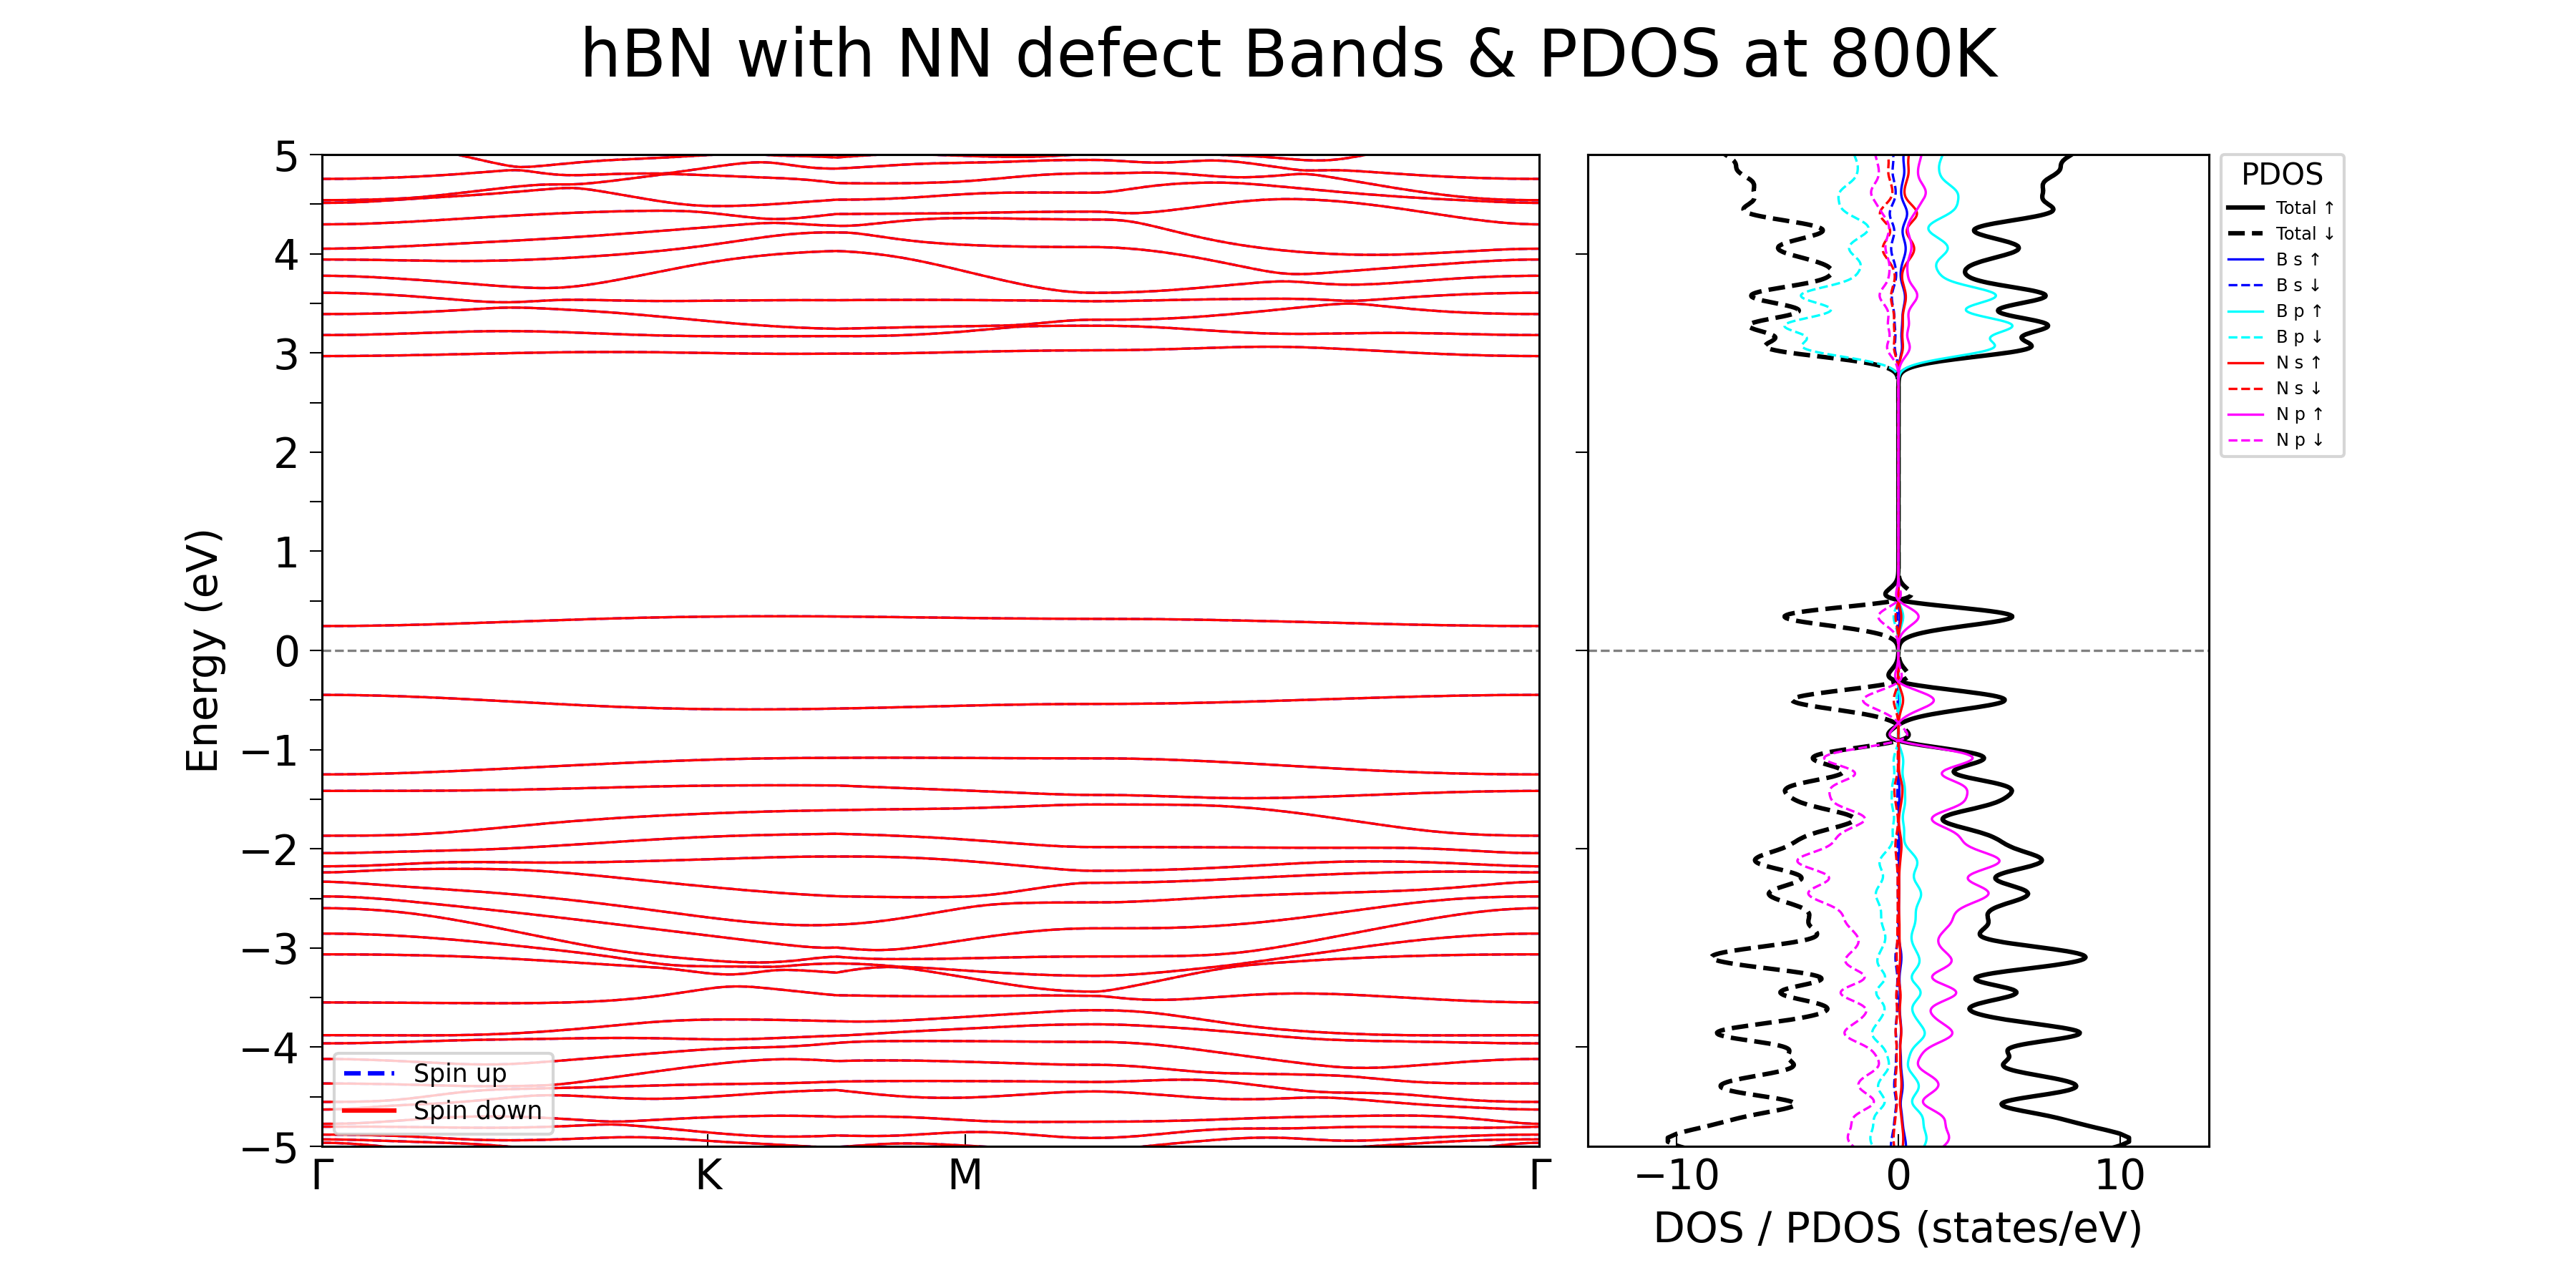
\includegraphics[width=0.95\textwidth]{gambar_hasil/simple_bands_pdos_NN_800K.png}
    \caption{Struktur pita elektronik dan PDOS untuk monolayer hBN dengan cacat N\textsubscript{B} pada 800 K. Terlihat tingkat cacat di dalam celah pita.}
    \label{fig:hbn_NN_800K}
\end{figure}
\begin{figure}[htbp!] % PERUBAHAN: Ukuran gambar diperbesar
    \centering
    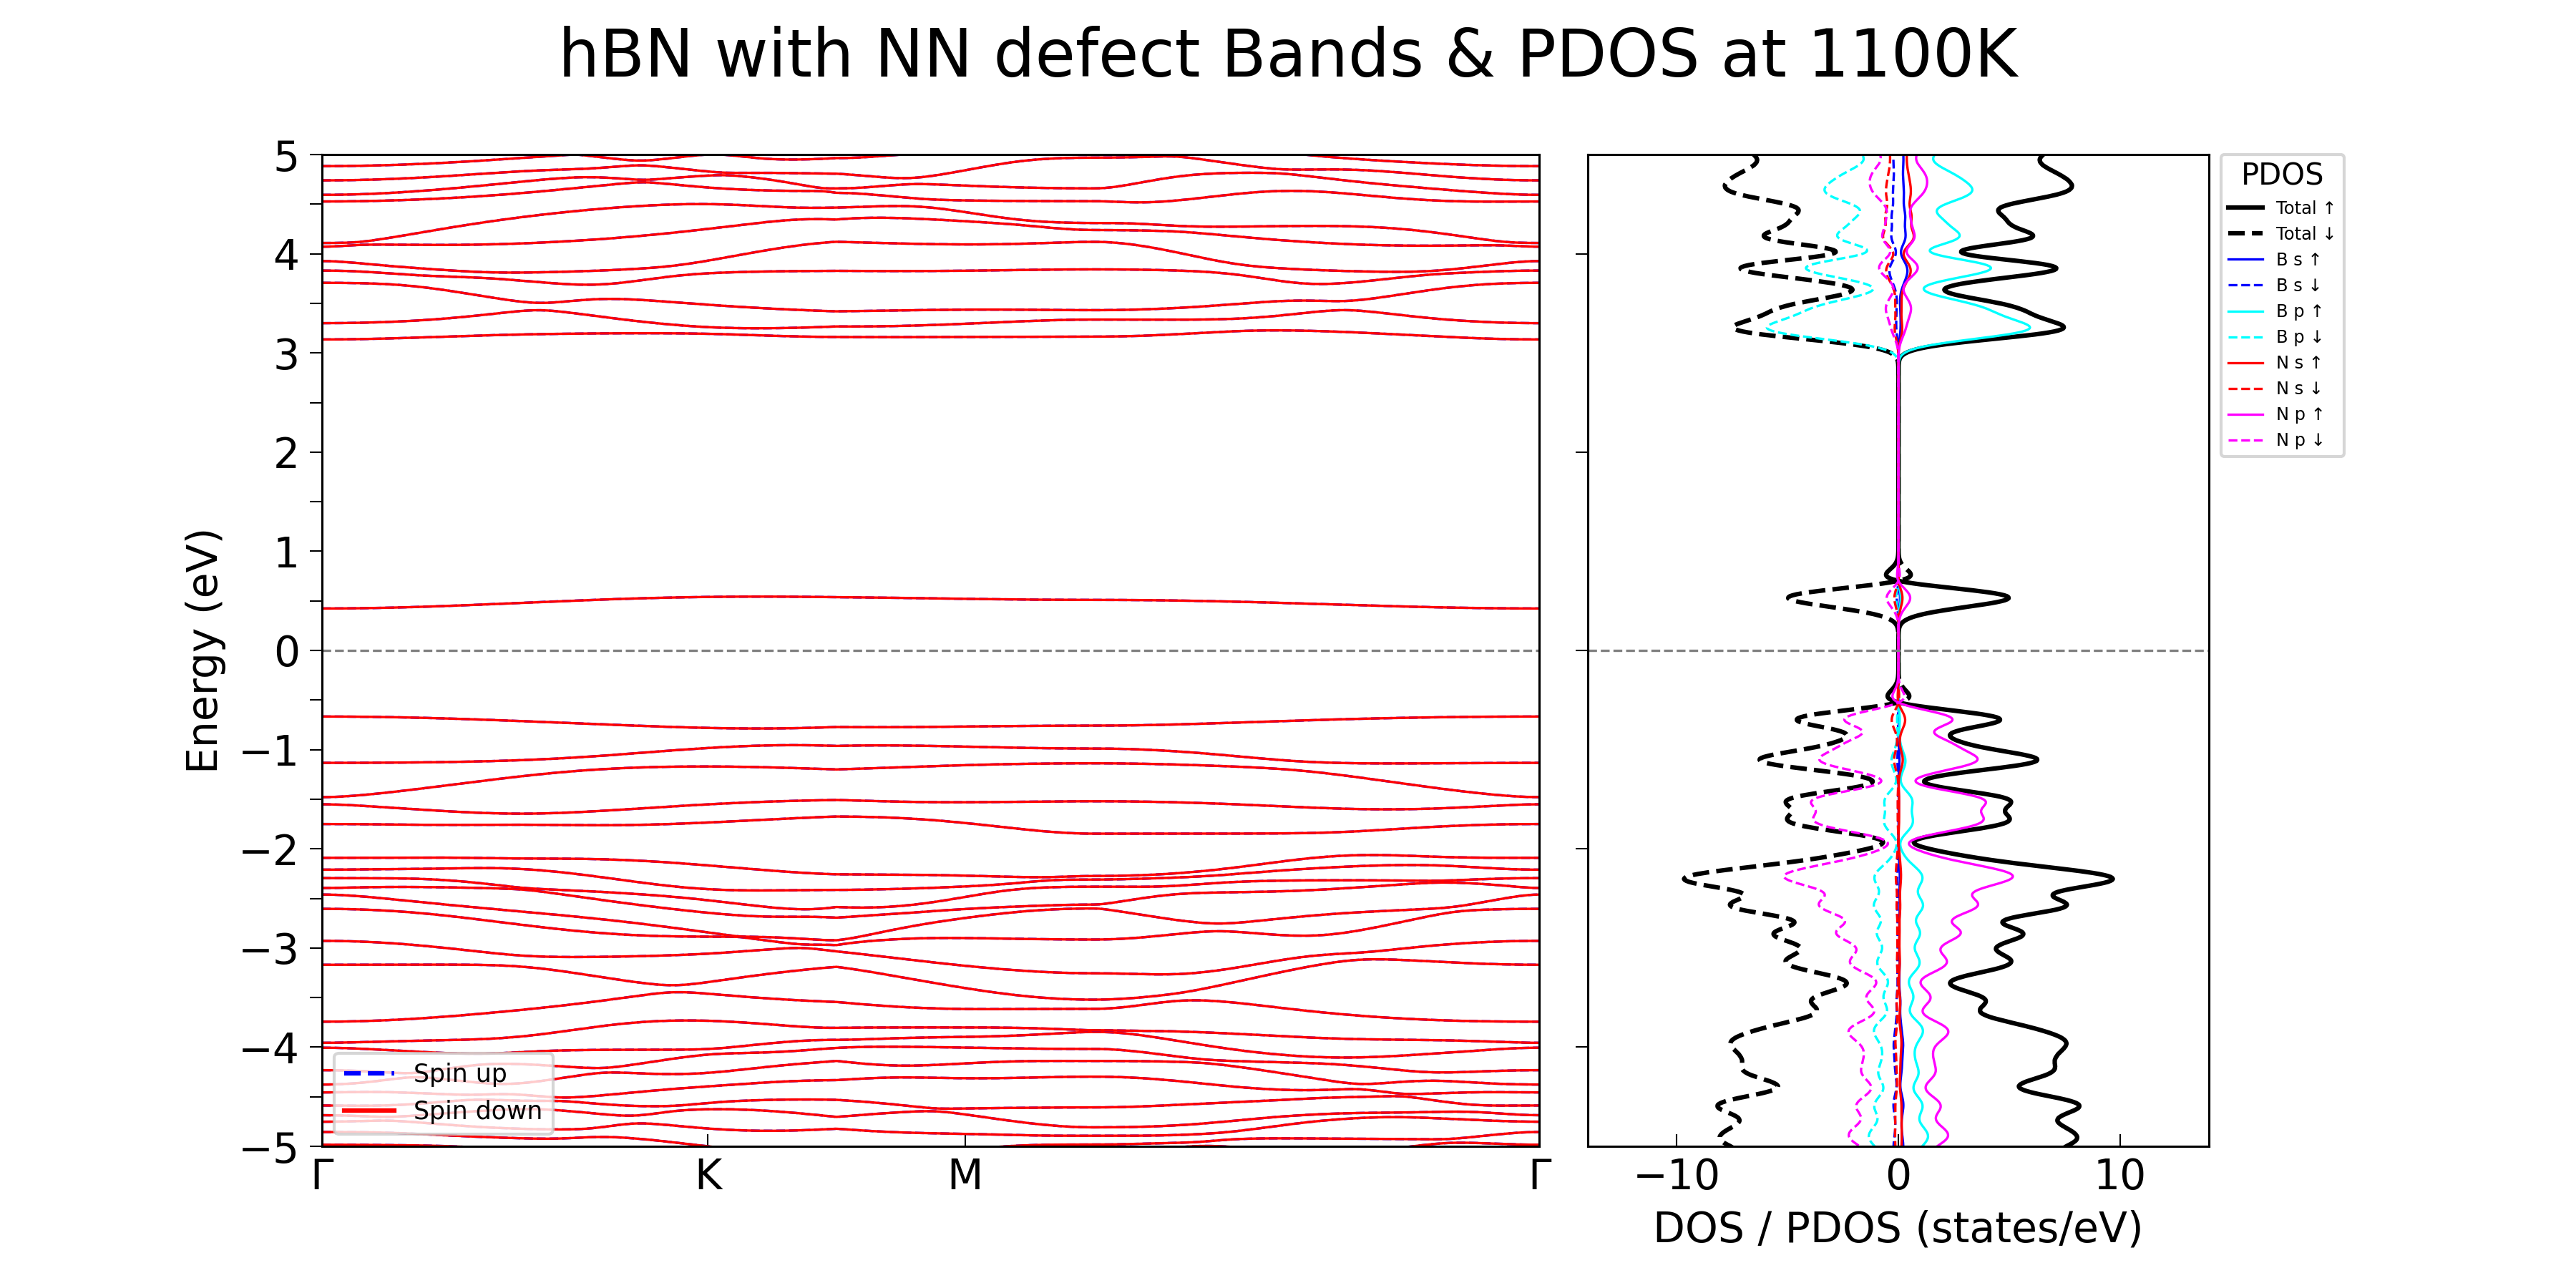
\includegraphics[width=0.95\textwidth]{gambar_hasil/simple_bands_pdos_NN_1100K.png}
    \caption{Struktur pita elektronik dan PDOS untuk monolayer hBN dengan cacat N\textsubscript{B} pada 1100 K. Celah pita efektif melebar menjadi $1.089$ eV.}
    \label{fig:hbn_NN_1100K}
\end{figure}
\begin{figure}[htbp!] % PERUBAHAN: Ukuran gambar diperbesar
    \centering
    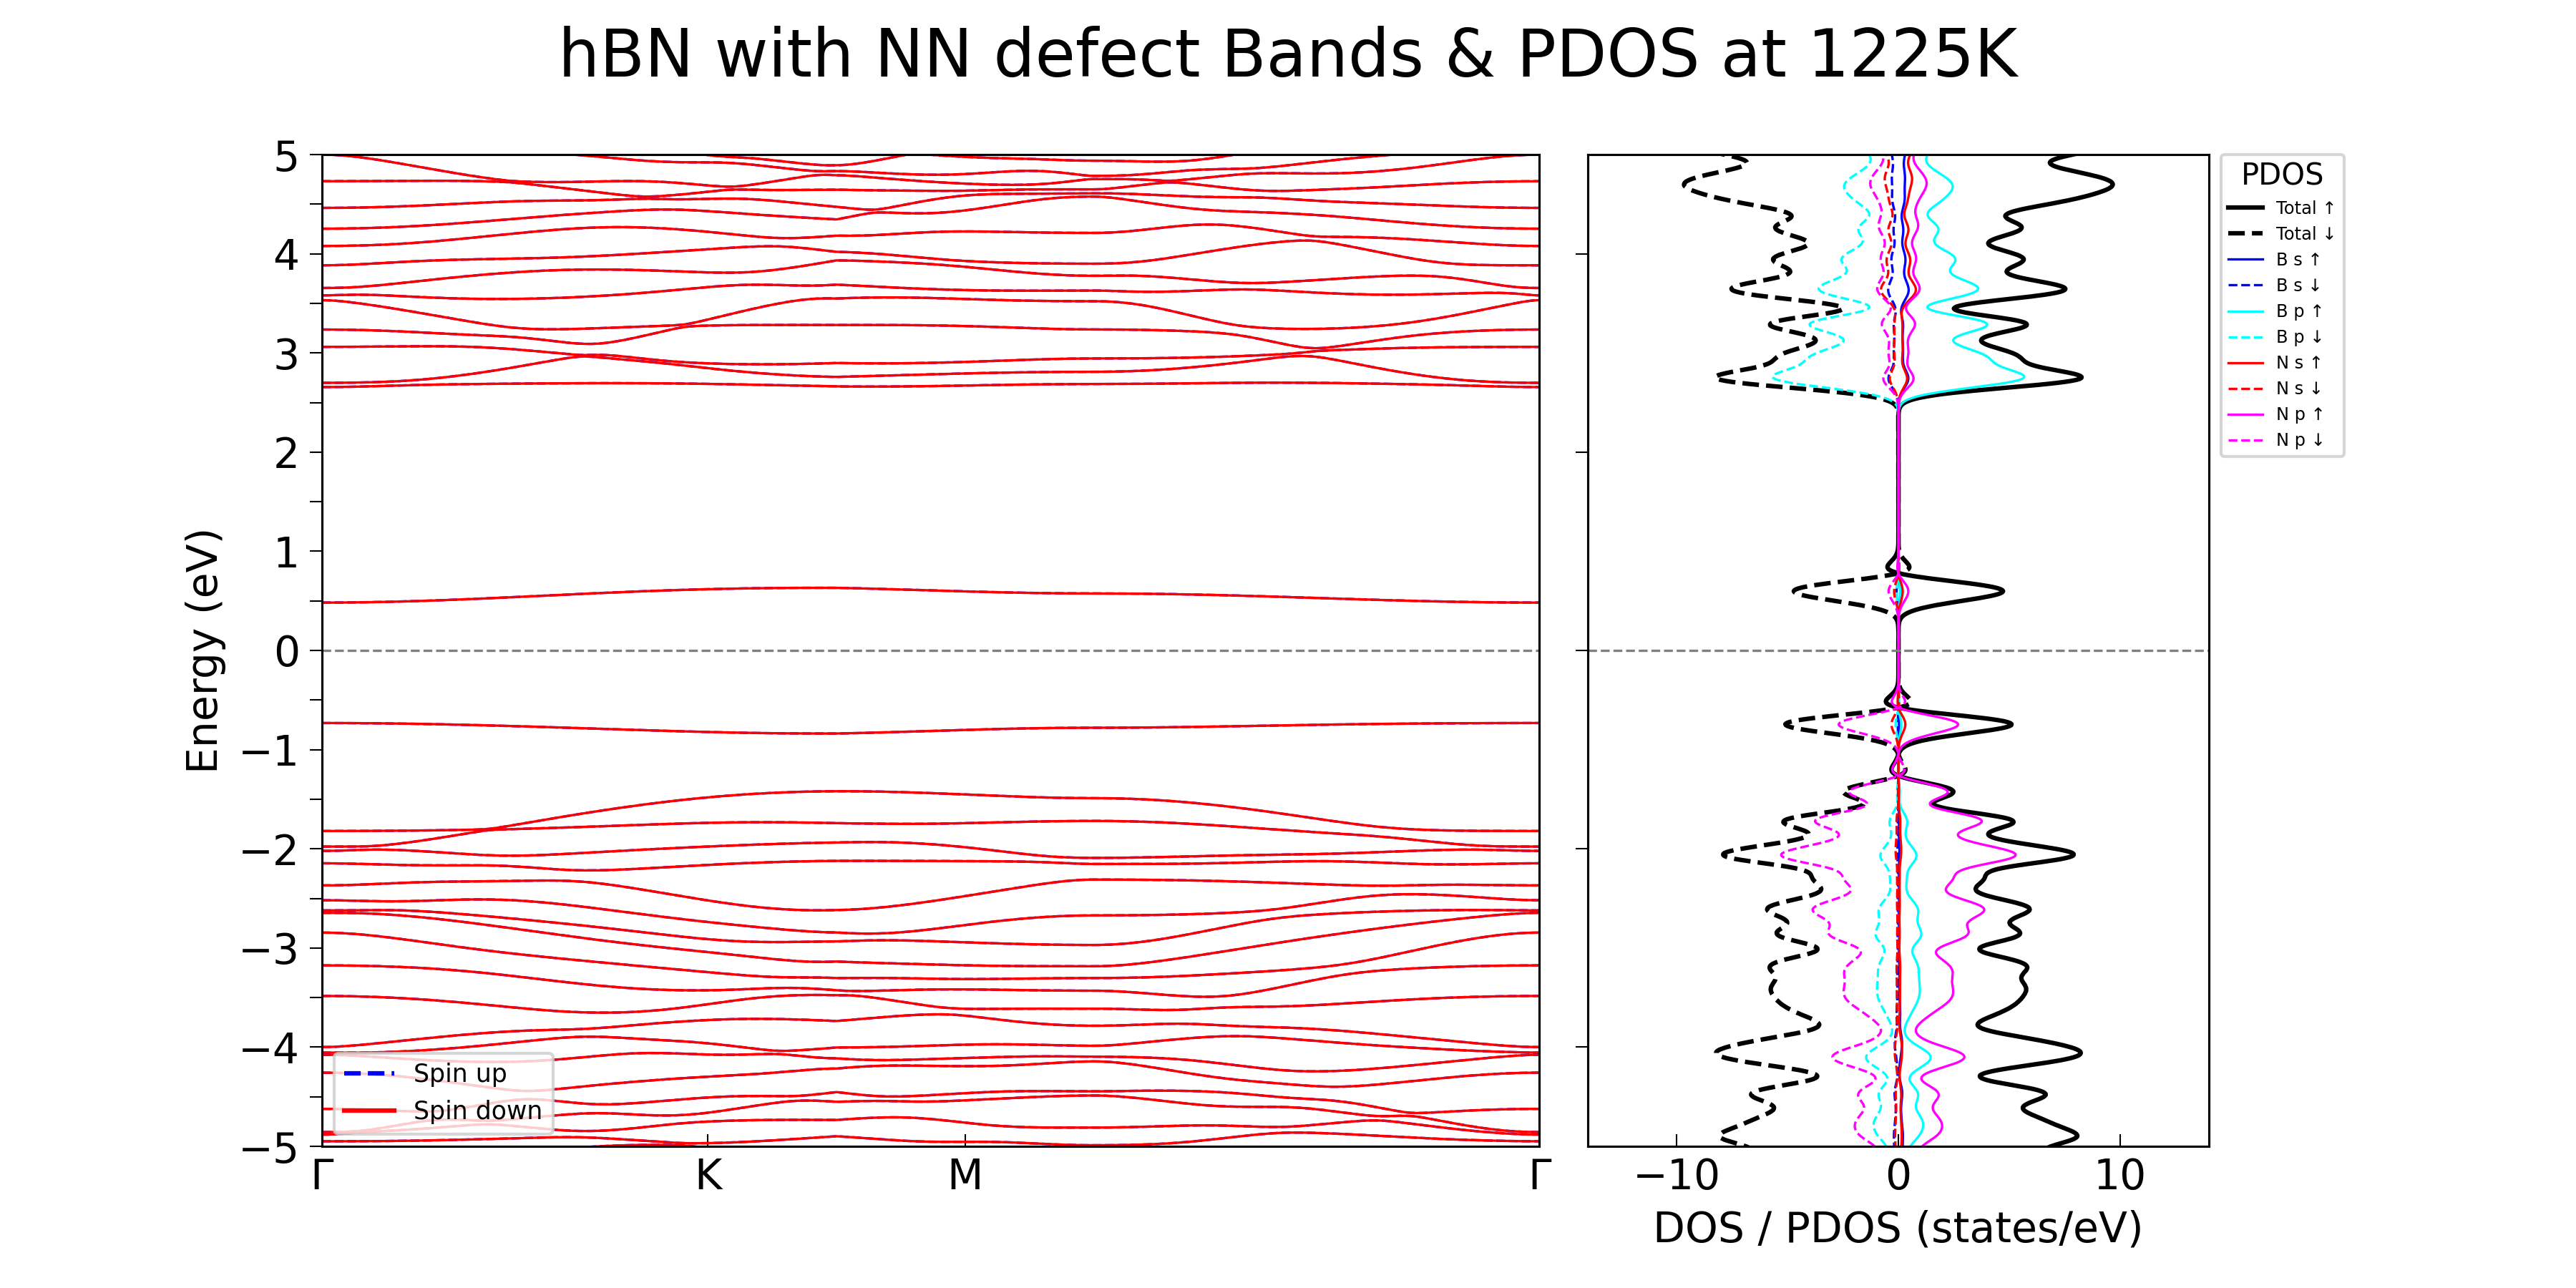
\includegraphics[width=0.95\textwidth]{gambar_hasil/simple_bands_pdos_NN_1225K.png}
    \caption{Struktur pita elektronik dan PDOS untuk monolayer hBN dengan cacat N\textsubscript{B} pada 1225 K. Celah pita terus melebar menjadi $1.214$ eV.}
    \label{fig:hbn_NN_1225K}
\end{figure}

Tren yang paling menonjol, seperti yang dirangkum dalam Tabel \ref{tab:hbn_defek_nb} dan diilustrasikan dari Gambar \ref{fig:hbn_NN_800K} hingga \ref{fig:hbn_NN_1225K}, adalah ketergantungan temperatur yang anomali dari celah pita.
Berlawanan dengan hBN murni, celah pita pada sistem dengan cacat N\textsubscript{B} justru \emph{meningkat} dengan kenaikan temperatur, dari $0.694$ eV pada 800 K menjadi $1.214$ eV pada 1225 K. Perilaku \emph{blueshift} anomali ini menunjukkan adanya mekanisme fisika yang berbeda secara fundamental.
Fenomena ini dapat dijelaskan oleh kopling elektron-fonon yang terlokalisasi. Celah pita efektif sekarang ditentukan oleh pemisahan energi antara keadaan cacat terisi dan tak terisi.
Keadaan-keadaan ini, karena sifatnya yang terlokalisasi di sekitar situs N\textsubscript{B}, sangat sensitif terhadap distorsi struktural lokal.
Vibrasi kisi (fonon) yang diaktifkan oleh suhu tinggi menyebabkan perubahan dinamis pada panjang ikatan dan sudut di sekitar cacat.
Untuk cacat N\textsubscript{B}, konfigurasi atomik yang terdistorsi oleh fonon ini secara kebetulan menghasilkan pemisahan energi yang lebih besar antara tingkat-tingkat cacat.
Dengan kata lain, fonon tidak lagi hanya menyebabkan "pencorengan" potensial global, tetapi secara aktif "memahat" lanskap energi lokal di sekitar cacat dengan cara yang memperlebar celah pitanya.
Sistem ini tetap non-magnetik di seluruh rentang temperatur yang diselidiki.

\subsubsection{Analisis Visual Kerapatan Muatan dan Spin untuk Cacat N\textsubscript{B}}
\label{subsec:hbn_NN_density_analysis}
Visualisasi distribusi elektron untuk sistem dengan cacat N\textsubscript{B} (Gambar \ref{fig:hbn_NN_density}) memberikan pemahaman yang lebih dalam tentang asal-usul perilaku elektroniknya yang unik.
\begin{figure}[htbp!] % PERUBAHAN: Ukuran gambar diperbesar
  \centering
  \begin{subfigure}[b]{0.49\textwidth}
    \centering
    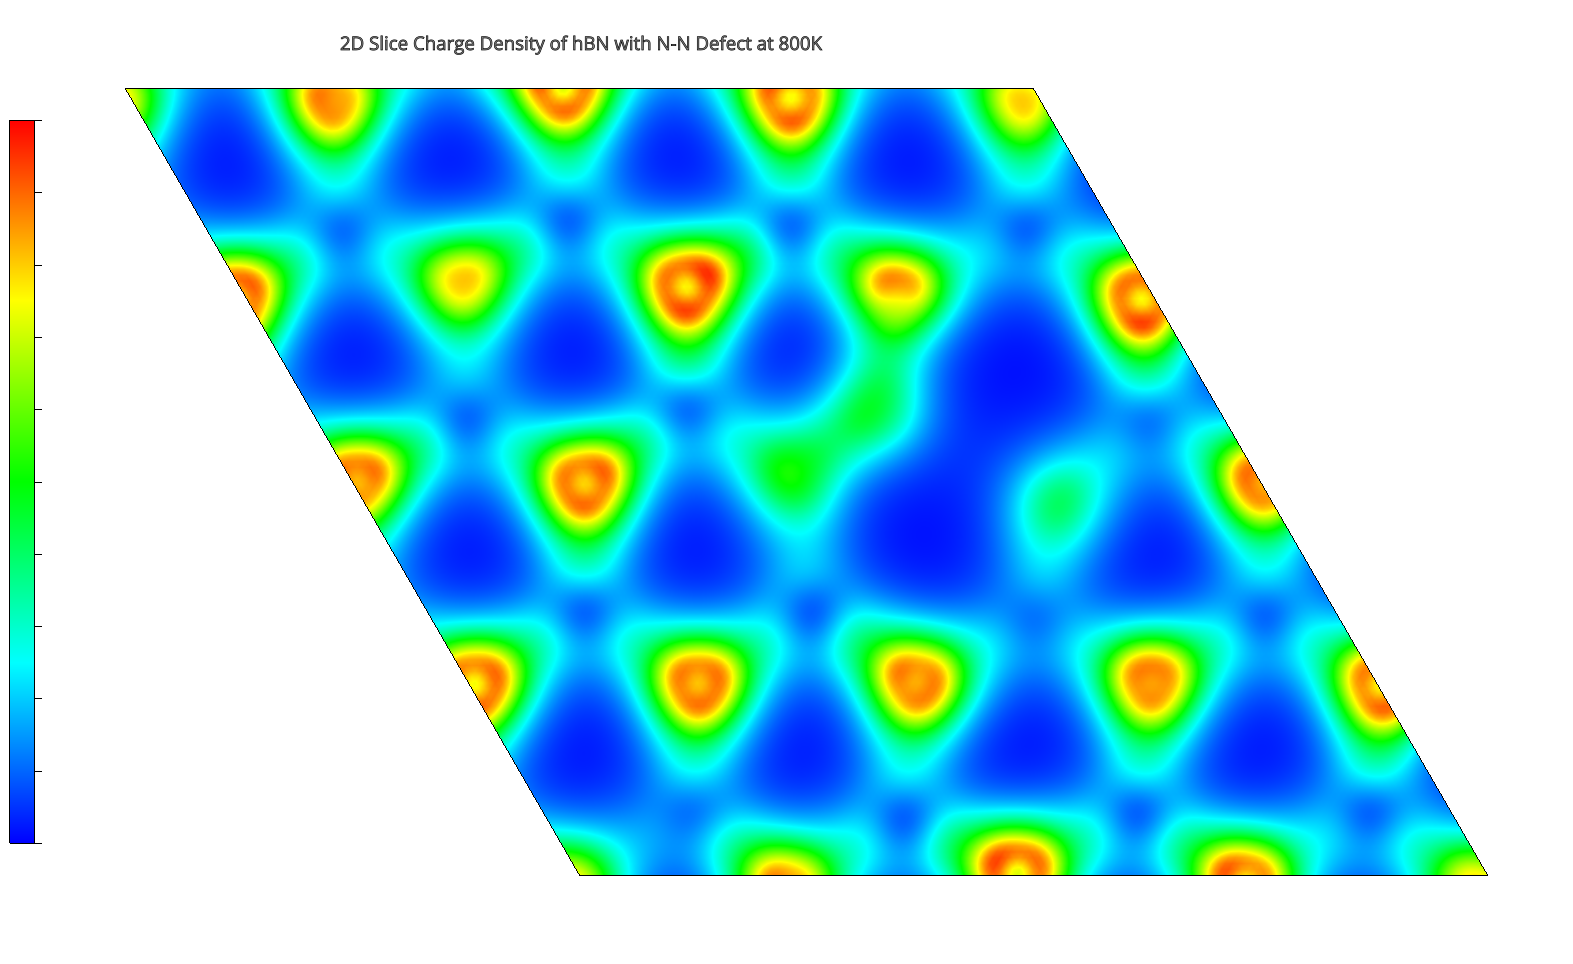
\includegraphics[width=\linewidth]{hBN_rho_NN_800K.png}
    \caption{Kerapatan Muatan, 800 K}
    \label{subfig:rho_nn_800k}
  \end{subfigure}\hfill
  \begin{subfigure}[b]{0.49\textwidth}
    \centering
    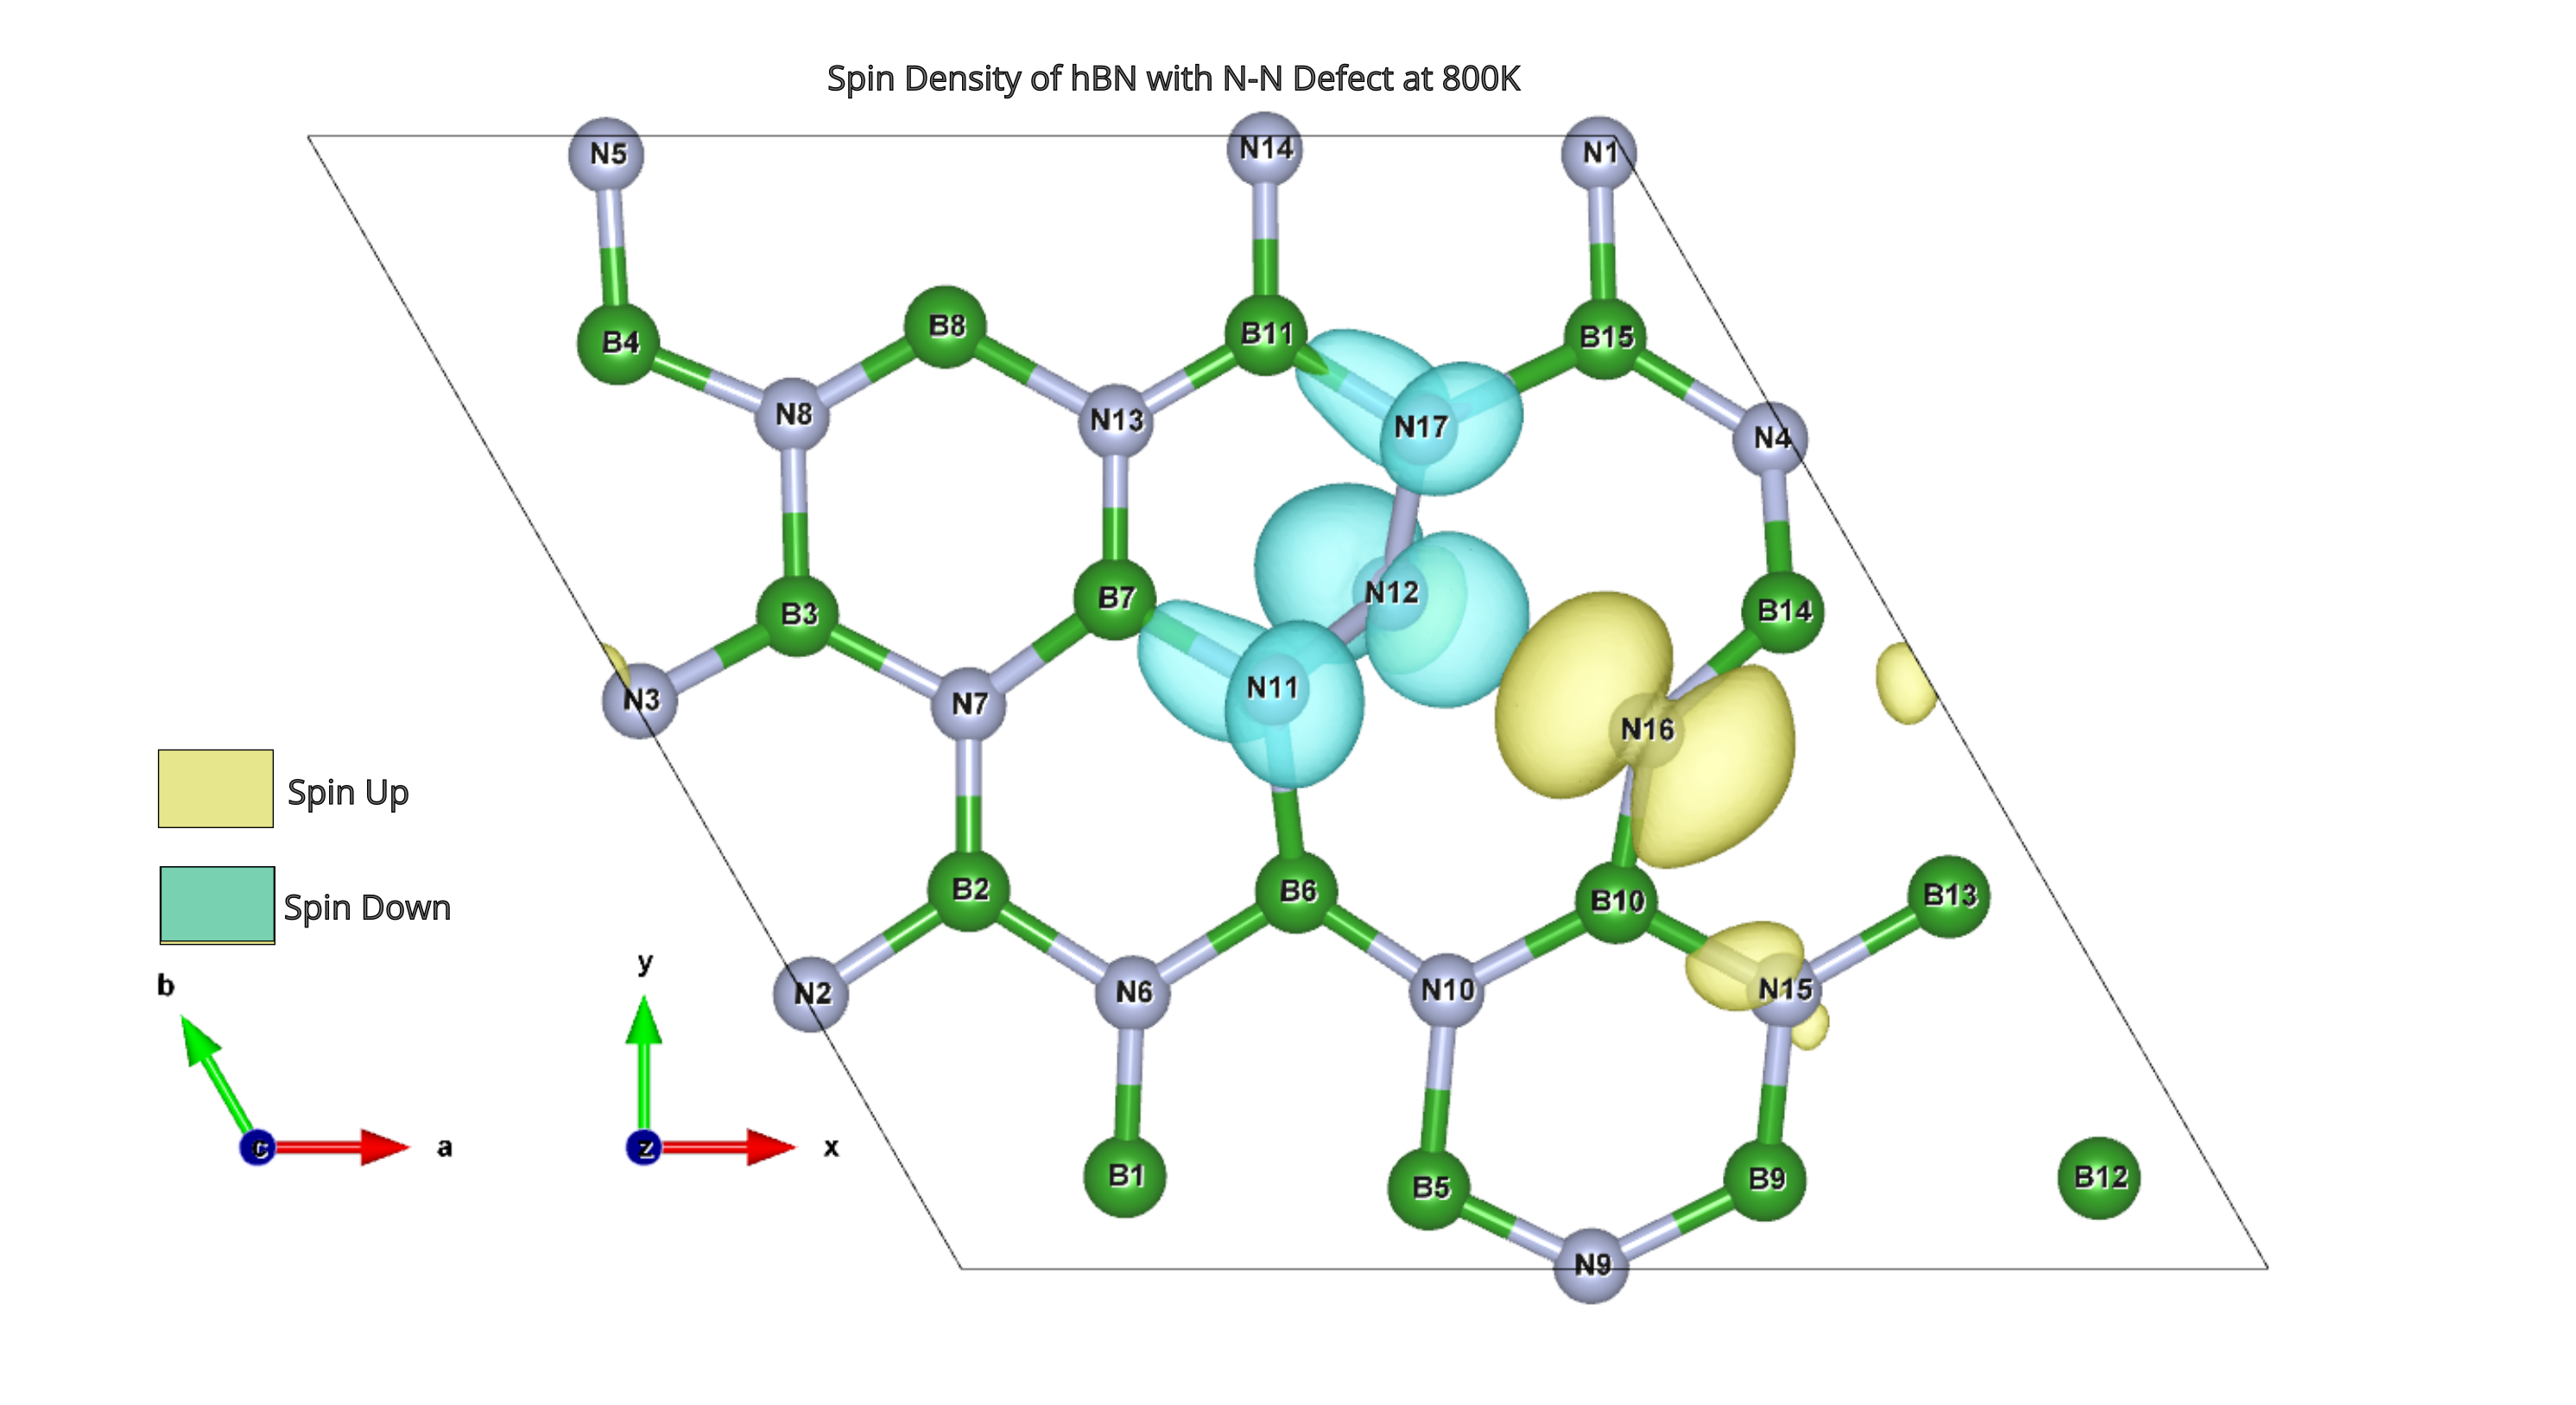
\includegraphics[width=\linewidth]{hBN_spin_NN_800K.png}
    \caption{Kerapatan Spin, 800 K}
    \label{subfig:spin_nn_800k}
  \end{subfigure}
  \vspace{1em}

  \begin{subfigure}[b]{0.49\textwidth}
    \centering
    \includegraphics[width=\linewidth]{hBN_rho_NN_1100K.png}
    \caption{Kerapatan Muatan, 1100 K}
    \label{subfig:rho_nn_1100k}
  \end{subfigure}\hfill
  \begin{subfigure}[b]{0.49\textwidth}
    \centering
    \includegraphics[width=\linewidth]{hBN_spin_NN_1100K.png}
    \caption{Kerapatan Spin, 1100 K}
    \label{subfig:spin_nn_1100k}
  \end{subfigure}
  \vspace{1em}

  \begin{subfigure}[b]{0.49\textwidth}
    \centering
    \includegraphics[width=\linewidth]{hBN_rho_NN_1225K.png}
    \caption{Kerapatan Muatan, 1225 K}
    \label{subfig:rho_nn_1225k}
  \end{subfigure}\hfill
  \begin{subfigure}[b]{0.49\textwidth}
    \centering
    \includegraphics[width=\linewidth]{hBN_spin_NN_1225K.png}
    \caption{Kerapatan Spin, 1225 K}
    \label{subfig:spin_nn_1225k}
  \end{subfigure}
  \caption{Visualisasi 2D dari kerapatan muatan total (kiri) dan kerapatan spin (kanan) untuk monolayer hBN dengan cacat N\textsubscript{B} pada 800 K, 1100 K, dan 1225 K. Kehadiran cacat menciptakan perturbasi lokal yang jelas pada kerapatan muatan. Warna merah pada kerapatan muatan menunjukkan akumulasi elektron, sedangkan warna biru menunjukkan deplesi. Untuk kerapatan spin, warna biru menunjukkan spin down dan warna kuning menunjukan spin up.}
  \label{fig:hbn_NN_density}
\end{figure}

Plot kerapatan muatan (Gambar \ref{fig:hbn_NN_density}a, c, e) dengan jelas menunjukkan bagaimana cacat N\textsubscript{B} mematahkan simetri translasi dari kisi hBN yang sempurna.
Terlihat adanya perturbasi yang sangat terlokalisasi pada distribusi muatan, yang berpusat di sekitar lokasi cacat.
Secara spesifik, pembentukan ikatan N-N antara atom nitrogen antisite dan tetangga nitrogennya menciptakan sebuah fitur elektronik yang berbeda dari ikatan B-N di sekitarnya.
Gangguan lokal inilah yang menjadi akar penyebab munculnya tingkat-tingkat energi cacat yang terlokalisasi di dalam celah pita, seperti yang diamati pada plot struktur pita (misalnya, Gambar \ref{fig:hbn_NN_800K}).
Lingkungan elektronik yang terbatas dan terisolasi ini sangat rentan terhadap perubahan geometri lokal, yang menjelaskan mengapa vibrasi termal (fonon) memiliki dampak yang begitu kuat dan spesifik (yaitu, \emph{blueshift}) pada tingkat energi cacat ini.
Serupa dengan kasus murni, plot kerapatan spin (Gambar \ref{fig:hbn_NN_density}b, d, f) menunjukkan polarisasi spin nol di seluruh sistem dan pada semua temperatur.
Meskipun Tabel \ref{tab:hbn_defek_nb} menunjukkan nilai magnetisasi absolut yang sangat kecil dan non-nol ($0.010 \mu_B$) pada 1225 K, visualisasi ini mengonfirmasi bahwa nilai tersebut adalah derau komputasi (\emph{computational noise}) dan bukan merupakan indikasi tatanan magnetik yang sebenarnya.
Ini adalah poin pembeda yang penting jika dibandingkan dengan cacat B\textsubscript{N}.
Bukti visual ini menunjukkan bahwa meskipun cacat N\textsubscript{B} secara signifikan mengubah struktur elektronik orbital, ia menciptakan keadaan yang secara elektronik "terpenuhi" atau "jenuh" yang tidak memiliki karakter elektron tak berpasangan yang diperlukan untuk memicu pemisahan spin (memenuhi kriteria Stoner).
Hal ini memperkuat kesimpulan bahwa fisika yang dominan dalam sistem N\textsubscript{B} diatur oleh interaksi muatan-fonon, bukan interaksi spin-fonon.

\subsection{Cacat B\textsubscript{N}: Induksi Magnetisme $d^0$ dan Kopling Spin-Fonon}
\label{subsec:hbn_defek_bn}
Cacat antisite B\textsubscript{N} menginduksi perubahan yang paling dramatis, yaitu kemunculan magnetisme yang bergantung pada temperatur.
Pada 800 K, sistem ini bersifat non-magnetik dengan celah pita $0.990$ eV (Gambar \ref{fig:hbn_BB_800K}).
Namun, seperti yang ditunjukkan pada Tabel \ref{tab:hbn_defek_bn}, transisi fasa magnetik terjadi pada temperatur yang lebih tinggi.
\begin{table}[htbp!] % STANDARISASI: Menggunakan [htbp!]
  \centering
  \caption{Sifat Elektronik dan Magnetik Monolayer hBN dengan Cacat Antisite B\textsubscript{N} sebagai Fungsi Temperatur.}
  \label{tab:hbn_defek_bn}
  % ANOTASI: \resizebox digunakan di sini sebagai solusi pragmatis untuk tabel
  % yang sangat lebar. Ini memastikan tabel pas di dalam lebar teks.
  % Namun, ini dapat menyebabkan ukuran font yang tidak konsisten dengan
  % teks lainnya. Untuk publikasi formal, alternatif seperti memformat ulang
  % tabel, menggunakan singkatan, atau menggunakan lingkungan 'sidewaystable'
  % (dari paket 'rotating') mungkin lebih disukai.
  \resizebox{\textwidth}{!}{%
  \begin{tabular}{lcccccccccc}
    \toprule
    Temperatur & VBM & CBM & $E_g$ Sistem & $E_F$ & Mag. Total & Mag. Abs. & Momen Orbital & Momen Orbital & Momen Orbital & Momen Orbital \\
    (K) & (eV) & (eV) & Total (eV) & (eV) & ($\mu_B$) & ($\mu_B$) & B-s ($\mu_B$) & B-p ($\mu_B$) & N-s ($\mu_B$) & N-p ($\mu_B$) \\
    \midrule
    800  & -0.633 & 0.357 & 0.990 & -0.249 & 0.000 & 0.000 & -0.000 & 0.000 & -0.000 & 0.000 \\
    1100 & -0.120 ($\downarrow$) & 0.301 ($\uparrow$)  & 0.421 & -0.410 & 0.150 & 0.230 &  0.003 & 0.010 & -0.000 & 0.001 \\
    1225 & -0.073 ($\uparrow$) & 0.243 ($\downarrow$)  & 0.316 & -0.622 & 1.850 & 2.320 &  0.057 & 0.009 & -0.022 & -0.002 \\
    \bottomrule
  \end{tabular}%
  }
\end{table}

\begin{figure}[htbp!] % PERUBAHAN: Ukuran gambar diperbesar
    \centering
    \includegraphics[width=0.95\textwidth]{gambar_hasil/simple_bands_pdos_BB_800K.png}
    \caption{Struktur pita elektronik dan PDOS untuk monolayer hBN dengan cacat B\textsubscript{N} pada 800 K. Sistem bersifat non-magnetik.}
    \label{fig:hbn_BB_800K}
\end{figure}
\begin{figure}[htbp!] % PERUBAHAN: Ukuran gambar diperbesar
    \centering
    \includegraphics[width=0.95\textwidth]{gambar_hasil/simple_bands_pdos_BB_1100K.png}
    \caption{Struktur pita elektronik dan PDOS untuk monolayer hBN dengan cacat B\textsubscript{N} pada 1100 K. Terjadi pemisahan spin (kanal spin-atas dan spin-bawah berbeda), menandakan kemunculan magnetisme ($0.150 \mu_B$).}
    \label{fig:hbn_BB_1100K}
\end{figure}
\begin{figure}[htbp!] % PERUBAHAN: Ukuran gambar diperbesar
    \centering
    \includegraphics[width=0.95\textwidth]{gambar_hasil/simple_bands_pdos_BB_1225K.png}
    \caption{Struktur pita elektronik dan PDOS untuk monolayer hBN dengan cacat B\textsubscript{N} pada 1225 K. Pemisahan spin menjadi sangat signifikan, dengan magnetisasi total meningkat tajam menjadi $1.850 \mu_B$.}
    \label{fig:hbn_BB_1225K}
\end{figure}

Kemunculan magnetisme pada sistem yang hanya terdiri dari unsur-unsur blok-p ini dikenal sebagai magnetisme $d^0$ \citep{zhou2019}.
Magnetisme ini tidak berasal dari orbital $d$ atau $f$ yang terisi sebagian, melainkan dari polarisasi spin elektron-elektron $p$ yang terlokalisasi akibat ketidakseimbangan elektron dan ikatan tak jenuh (\emph{dangling bonds}) yang diciptakan oleh cacat.
Cacat B\textsubscript{N} menciptakan keadaan elektronik terlokalisasi di dekat tingkat Fermi, yang jika kerapatannya cukup tinggi, dapat memicu polarisasi spin spontan untuk menurunkan energi total sistem (kriteria Stoner).
Temuan yang paling luar biasa adalah \emph{peningkatan} magnetisasi dengan suhu, dari nol pada 800 K menjadi $1.850 \mu_B$ pada 1225 K. Perilaku ini sangat tidak konvensional, karena energi termal ($k_B T$) biasanya berfungsi mengacaukan tatanan magnetik.
Fenomena ini menunjuk pada adanya mekanisme kopling spin-fonon (SPC) yang kuat \citep{Liu_2025}.
Hipotesisnya adalah sebagai berikut:
\begin{enumerate}
    \item Pada 800 K, distorsi termal pada kisi belum cukup kuat untuk membuat keadaan dasar magnetik lebih stabil daripada keadaan non-magnetik.
\item Seiring meningkatnya temperatur ke 1100 K dan 1225 K, moda-moda fonon beramplitudo lebih besar menjadi aktif.
\item Moda-moda fonon spesifik ini berinteraksi kuat dengan keadaan spin elektronik di sekitar cacat B\textsubscript{N}.
\item Interaksi ini berarti vibrasi kisi tidak lagi bertindak sebagai sumber kekacauan, tetapi secara aktif \emph{menciptakan dan menstabilkan} distorsi struktural lokal (misalnya, pemanjangan ikatan atau pengerutan) yang kondusif untuk polarisasi spin.
\end{enumerate}
Dengan kata lain, fonon menjadi bahan aktif yang memediasi transisi menuju fasa magnetik.
Temperatur yang lebih tinggi mendorong sistem lebih dalam ke fase magnetik yang lebih teratur, sebuah contoh menakjubkan dari bagaimana interaksi kolektif dapat memunculkan tatanan yang tidak terduga \citep{Pantazopoulos2024}.

\subsubsection{Bukti Visual Kopling Spin-Fonon dari Kerapatan Muatan dan Spin}
\label{subsec:hbn_BB_density_analysis}
Analisis kerapatan muatan dan spin untuk sistem B\textsubscript{N} (Gambar \ref{fig:hbn_BB_density}) memberikan bukti visual yang paling meyakinkan untuk mekanisme magnetisme yang diinduksi oleh temperatur.
Plot-plot ini menyajikan narasi visual tentang transisi fasa dari keadaan non-magnetik ke keadaan magnetik yang kuat.
\begin{figure}[htbp!] % PERUBAHAN: Ukuran gambar diperbesar
  \centering
  \begin{subfigure}[b]{0.49\textwidth}
    \centering
    \includegraphics[width=\linewidth]{hBN_rho_BB_800K.png}
    \caption{Kerapatan Muatan, 800 K}
    \label{subfig:rho_bb_800k}
  \end{subfigure}\hfill
  \begin{subfigure}[b]{0.49\textwidth}
    \centering
    \includegraphics[width=\linewidth]{hBN_spin_BB_800K.png}
    \caption{Kerapatan Spin, 800 K}
    \label{subfig:spin_bb_800k}
  \end{subfigure}
  \vspace{1em}

  \begin{subfigure}[b]{0.49\textwidth}
    \centering
    \includegraphics[width=\linewidth]{hBN_rho_BB_1100K.png}
    \caption{Kerapatan Muatan, 1100 K}
    \label{subfig:rho_bb_1100k}
  \end{subfigure}\hfill
  \begin{subfigure}[b]{0.49\textwidth}
    \centering
    \includegraphics[width=\linewidth]{hBN_spin_BB_1100K.png}
    \caption{Kerapatan Spin, 1100 K}
    \label{subfig:spin_bb_1100k}
  \end{subfigure}
  \vspace{1em}

  \begin{subfigure}[b]{0.49\textwidth}
    \centering
    \includegraphics[width=\linewidth]{hBN_rho_BB_1225K.png}
    \caption{Kerapatan Muatan, 1225 K}
    \label{subfig:rho_bb_1225k}
  \end{subfigure}\hfill
  \begin{subfigure}[b]{0.49\textwidth}
    \centering
    \includegraphics[width=\linewidth]{hBN_spin_BB_1225K.png}
    \caption{Kerapatan Spin, 1225 K}
    \label{subfig:spin_bb_1225k}
  \end{subfigure}
  \caption{Visualisasi 2D dari kerapatan muatan (kiri) dan kerapatan spin (kanan) untuk monolayer hBN dengan cacat B\textsubscript{N}. Warna merah pada kerapatan muatan menunjukkan akumulasi elektron, sedangkan warna biru menunjukkan deplesi. Untuk kerapatan spin, warna biru menunjukkan spin down dan warna kuning menunjukan spin up.}
  \label{fig:hbn_BB_density}
\end{figure}

Plot kerapatan muatan (Gambar \ref{fig:hbn_BB_density}a, c, e) menyoroti lingkungan elektronik yang sangat tidak stabil yang diciptakan oleh cacat B\textsubscript{N}.
Pembentukan ikatan B-B dan keberadaan atom nitrogen di sekitarnya yang kurang terkoordinasi menciptakan keadaan elektronik yang "tidak jenuh".
Lingkungan inilah yang rentan terhadap pemisahan spin, menyediakan keadaan sempit dengan kerapatan tinggi di dekat tingkat Fermi yang diperlukan untuk magnetisme $d^0$.
Naratif sesungguhnya terungkap dalam plot kerapatan spin. Pada 800 K (Gambar \ref{fig:hbn_BB_density}b), kerapatan spin adalah nol, yang secara visual mengonfirmasi keadaan dasar non-magnetik sistem, sejalan dengan data pada Tabel \ref{tab:hbn_defek_bn}.
Pada temperatur ini, energi termal tidak cukup untuk memicu mekanisme kopling spin-fonon.
Sebuah transisi dramatis terjadi pada 1100 K (Gambar \ref{fig:hbn_BB_density}d). Di sini, kita menyaksikan \emph{kemunculan} polarisasi spin.
Kantong-kantong kerapatan spin-atas (merah) dan spin-bawah (biru) yang terlokalisasi muncul, terutama pada atom-atom nitrogen yang bertetangga dengan situs cacat B\textsubscript{N}.
Ini adalah "bukti tak terbantahkan" (\emph{smoking gun}) dari onset magnetisme $d^0$, yang secara visual menunjukkan bahwa momen magnetik berasal dari polarisasi orbital $p$ pada atom-atom non-logam ini.
Ini adalah bukti visual pertama bahwa temperatur mulai \emph{menginduksi} tatanan magnetik, bukan menghancurkannya.
Pada 1225 K (Gambar \ref{fig:hbn_BB_density}f), fenomena ini mengalami \emph{amplifikasi} yang signifikan.
Intensitas warna (menunjukkan besarnya polarisasi spin) dan jangkauan spasial dari daerah yang terpolarisasi spin meningkat secara dramatis.
Ini memberikan bukti visual yang tak terbantahkan untuk hipotesis kopling spin-fonon.
Peningkatan energi termal menggerakkan moda fonon beramplitudo lebih besar—sebuah fenomena yang telah diisyaratkan oleh nilai MSD yang tinggi untuk sistem ini (Bagian \ref{subsec:md_rdf_msd}).
Alih-alih mengacaukan tatanan magnetik, vibrasi-vibrasi ini secara aktif menstabilkan distorsi geometris lokal yang tidak hanya memungkinkan tetapi juga \emph{memperkuat} polarisasi spin.
Fenomena kontra-intuitif di mana "gangguan" (vibrasi termal) mengarah pada "tatanan" (magnetisme) kini terkonfirmasi secara visual.

\section{Sintesis: Keterkaitan antara Dinamika Struktur, Stabilitas Termal, dan Sifat Kuantum}
\label{sec:diskusi_komprehensif}
Analisis yang telah dipaparkan mengungkapkan sebuah narasi yang kaya tentang bagaimana struktur, stabilitas, dan sifat kuantum saling terkait erat dalam monolayer hBN.
Dengan menggabungkan wawasan dari simulasi MD dan kalkulasi DFT, kita dapat membangun gambaran komprehensif tentang fisika yang mendasari perilaku material ini di bawah pengaruh temperatur dan cacat.
\subsection{Korelasi Struktur-Sifat: Dari RDF/MSD ke Elektronik}
\label{subsec:korelasi_struktur_md_dft}
Alur kerja multi-skala yang digunakan dalam penelitian ini menyoroti hubungan sebab-akibat yang krusial: dinamika struktural pada skala pikosekon (ditangkap oleh MD) secara langsung menentukan sifat elektronik keadaan dasar (dihitung oleh DFT).
\begin{itemize}
    \item Untuk hBN murni, analisis RDF dan MSD (Bagian \ref{subsec:md_rdf_msd}) menunjukkan sistem yang relatif teratur dan stabil.
Sifat elektronik yang dihasilkan (Bagian \ref{subsec:hbn_murni_termal}) mencerminkan respons "global" dari kisi yang teratur ini terhadap eksitasi termal, yaitu pergeseran merah normal yang didorong oleh kopling elektron-fonon.
Ketiadaan polarisasi spin pada Gambar \ref{fig:hbn_pure_density} melengkapi gambaran ini.
    \item Untuk hBN dengan cacat N\textsubscript{B}, RDF menunjukkan gangguan struktural lokal yang lebih besar.
Lingkungan yang terdistorsi secara statis di sekitar cacat ini, yang divisualisasikan dalam Gambar \ref{fig:hbn_NN_density}, menjadi tuan rumah bagi keadaan elektronik terlokalisasi.
Respons termal dari sistem ini tidak lagi global, melainkan didominasi oleh bagaimana fonon berinteraksi dengan keadaan cacat lokal ini, menghasilkan pergeseran biru anomali melalui mekanisme kopling elektron-fonon terlokalisasi (Bagian \ref{subsec:hbn_defek_nb}).
\item Yang paling krusial, untuk hBN dengan cacat B\textsubscript{N}, analisis MSD (Bagian \ref{subsec:md_rdf_msd}) mengungkapkan mobilitas atomik tertinggi dan ketidakstabilan dinamis yang paling signifikan.
"Ketidakstabilan" ini bukanlah kegagalan, melainkan ciri khas fisik yang penting.
Mobilitas atomik yang tinggi ini adalah jejak makroskopis dari vibrasi kisi (fonon) beramplitudo besar.
Bukti visual dari kerapatan spin pada Gambar \ref{fig:hbn_BB_density} kini secara langsung menunjukkan bagaimana vibrasi kisi beramplitudo besar ini menjadi "mesin" yang mendorong dan menstabilkan keadaan magnetik pada temperatur tinggi (Bagian \ref{subsec:hbn_defek_bn}).
Dengan demikian, hasil MSD memberikan bukti struktural yang mendukung mekanisme magnetisme yang diinduksi oleh fonon.
\end{itemize}

\subsection{Ringkasan Mekanisme Fisik dan Implikasi}
\label{subsec:ringkasan_implikasi}
Penelitian ini mengungkap tiga narasi fisika yang berbeda dan bergantung pada sistem, yang dirangkum dalam Tabel \ref{tab:konsolidasi_eg_mag}:
\begin{enumerate}
    \item hBN Murni: Perilaku didominasi oleh kopling elektron-fonon global, menghasilkan renormalisasi celah pita termal yang normal (\emph{redshift}).
\item hBN + Cacat N\textsubscript{B}: Perilaku didominasi oleh kopling elektron-fonon terlokalisasi pada keadaan cacat, menghasilkan respons termal yang anomali (\emph{blueshift}).
\item hBN + Cacat B\textsubscript{N}: Perilaku didominasi oleh kopling spin-fonon yang kuat, menghasilkan fenomena luar biasa berupa magnetisme $d^0$ yang diinduksi dan diperkuat oleh temperatur.
\end{enumerate}

Meskipun validitas kuantitatif dari beberapa temuan (misalnya, besaran momen magnetik) bergantung pada akurasi metodologi komputasi yang digunakan, tren kualitatif yang diamati memiliki implikasi penting.
Kemampuan untuk menyetel tidak hanya nilai celah pita tetapi juga koefisien temperaturnya melalui rekayasa cacat membuka peluang untuk perangkat optoelektronik dengan stabilitas termal yang dirancang khusus.
Lebih jauh lagi, induksi magnetisme yang dapat dikontrol oleh temperatur pada material non-magnetik intrinsik seperti hBN menunjukkan potensi besar untuk aplikasi spintronik generasi baru, seperti sensor termo-magnetik atau sakelar spin yang diaktifkan oleh panas.
Secara keseluruhan, penelitian ini menunjukkan bahwa monolayer hBN jauh dari sekadar substrat isolator pasif;
ia adalah platform material yang kaya akan fisika kompleks dan dapat direkayasa untuk fungsionalitas kuantum yang baru.
\begin{table}[htbp!] % STANDARISASI: Menggunakan [htbp!]
  \centering
  \caption{Tinjauan Konsolidasi Celah Pita Energi dan Magnetisasi Total untuk Semua Sistem yang Dikaji.}
  \label{tab:konsolidasi_eg_mag}
  \begin{tabular}{llcc}
    \toprule
    Sistem & Temperatur (K) & Celah Pita Energi ($E_g$) (eV) & Magnetisasi Total ($\mu_B$) \\
    \midrule
    hBN Murni & Pristine & 4.446 & 0.000 \\
              & 800      & 4.415 & 0.000 \\
              & 1100     & 4.328 & 0.000 \\
              & 1225     & 4.069 & 0.000 \\
    \midrule
    hBN + Cacat N\textsubscript{B} & 800  & 0.694 &  0.000 \\
                                  & 1100 & 1.089 &  0.000 \\
                                  & 1225 & 1.214 &  0.000 \\
    \midrule
    hBN + Cacat B\textsubscript{N} & 800  & 0.990 &  0.000 \\
                                  & 1100 & 0.421 &  0.150 \\
                                  & 1225 & 0.316 &  1.850 \\
    \bottomrule
  \end{tabular}
\end{table}
    %%%%%%%%%%%%%%%%%%%%%%%%%%%%%%%%%%%%%%%%%%%%%%%%%%%%%%%%%%%%%%%%%%%%%%
% BAB PENUTUP
%=====================================================================
\renewcommand{\thechapter}{\Roman{chapter}}
\addtocontents{toc}{\vskip10pt}
\chapter{PENUTUP}
\renewcommand{\thechapter}{\arabic{chapter}}
%---------------------------------------------------------------------

\section{Kesimpulan}
\label{sec:kesimpulan}
Penelitian ini menunjukkan bahwa efek termal dan defek titik secara sinergis memodulasi sifat elektronik dan magnetik monolayer hBN.
Telah terbukti bahwa hBN murni mengalami pergeseran merah (redshift) celah pita yang normal akibat kopling elektron-fonon.
Sebaliknya, defek antisite N$_B$ menyebabkan pergeseran biru (blueshift) yang anomali, menunjukkan adanya mekanisme fisika yang terlokalisasi di sekitar defek.
Temuan paling krusial adalah induksi magnetisme $d^0$ oleh defek B$_N$, yang secara tak terduga menguat pada temperatur tinggi.
Fenomena ini mengindikasikan adanya kopling spin-fonon yang kuat, di mana distorsi kisi termal secara aktif menstabilkan keadaan magnetik.
Keandalan kuantitatif dari temuan ini, khususnya besaran momen magnetik, bergantung pada akurasi metodologi komputasi yang digunakan.

\section{Saran}
\label{sec:saran}
Untuk penelitian selanjutnya, disarankan untuk memvalidasi temuan ini dengan metode komputasi yang lebih akurat guna meningkatkan keandalan kuantitatif.
Ini mencakup penggunaan \textbf{potensial antar-atom berbasis machine-learning (MLIPs)} untuk simulasi dinamika molekuler yang lebih realistis dan penerapan \textbf{fungsional hibrid (seperti HSE06) atau metode GW} untuk perhitungan sifat elektronik yang lebih presisi.
Selain itu, analisis energi pembentukan defek serta penggunaan supercell yang lebih besar sangat direkomendasikan untuk mengkonfirmasi stabilitas termodinamika defek dan menghilangkan potensi interaksi antar citra periodik, sehingga memastikan bahwa sifat-sifat yang teramati bersifat intrinsik dan bukan artefak komputasi.
    
%---------------------------------------------------------------------
%   DAFTAR PUSTAKA
%---------------------------------------------------------------------

    \addtocontents{toc}{\vskip10pt}
    \renewcommand{\bibname}{DAFTAR PUSTAKA}
    \addcontentsline{toc}{chapter}{DAFTAR PUSTAKA}
    %\bibliographystyle{unsrt} % untuk style dengan nomor
    \bibliographystyle{plainnat} % untuk style dengan nama
    \bibliography{pustaka}
    
%---------------------------------------------------------------------
%   APPENDIX
%---------------------------------------------------------------------

    {
    \appendix
    \addtocontents{toc}{\vskip10pt}
    \renewcommand{\chaptername}{LAMPIRAN}
    %%%%%%%%%%%%%%%%%%%%%%%%%%%%%%%%%%%%%%%%%%%%%%%%%%%%%%%%%%%%%%%%%%%%%%
% 
%%%%%%%%%%%%%%%%%%%%%%%%%%%%%%%%%%%%%%%%%%%%%%%%%%%%%%%%%%%%%%%%%%%%%%

\chapter{Lampiran}

%---------------------------------------------------------------------


\section{Kode dan Keluaran Hasil Simulasi dan Komputasi MD dan DFT }
Kode komputasi MD dan DFT menggunakan LAMMPS dan Quantum Espresso dapat diakses dengan seijin penulis dan pembimbing pada link github berikut \href{https://github.com/mhkry412/Kode_Kalkulasi_hBN_DFT_MD}{github/mhkry412/kode-kalkulasi-hBN-DFT-MD}




%%%%%%%%%%%%%%%%%%%%%%%%%%%%%%%%%%%%%%%%%%%%%%%%%%%%%%%%%%%%%%%%%%%%%%
    %\input{./halaman-belakang/lampiran/lampiranB}
    }
%---------------------------------------------------------------------
%   BIOGRAFI PENULIS
%---------------------------------------------------------------------

    %%%%%%%%%%%%%%%%%%%%%%%%%%%%%%%%%%%%%%%%%%%%%%%%%%%%%%%%%%%%%%%%%%%%%%
%%%%%%%%%%%%%%%%%%%%%%%%%%%%%%%%%%%%%%%%%%%%%%%%%%%%%%%%%%%%%%%%%%%%%%
% BIOGRAFI PENULIS
%=====================================================================
\renewcommand{\thechapter}{\Roman{chapter}}
\addtocontents{toc}{\vskip10pt}
\chapter*{BIOGRAFI PENULIS}
\renewcommand{\thechapter}{\arabic{chapter}}
%---------------------------------------------------------------------

\begin{wrapfigure}{l}{.35\textwidth}
  \begin{center}
    \vspace{-20pt} % Silahkan disesuaikan apabila space di atas gambar terlalu kecil/besar
    \includegraphics[width=.30\textwidth]{./gambar/Pas Foto Handar Ori.JPG}
    \vspace{-20pt} % Silahkan disesuaikan apabila space di bawah gambar terlalu kecil/besar
  \end{center}
\end{wrapfigure}

\noindent Nama lengkap penulis Hanandaru Mahaputra Purwanto, dengan nama panggilan Handar. Penulis dilahirkan di Surabaya, 23 September 2002, merupakan anak pertama dari dua bersaudara. Penulis telah menempuh pendidikan formal di SMPK Tegaljaya Badung dan SMAK Kolese Santo Yusup Malang. Setelah lulus dari SMA pada tahun 2021 penulis diterima di Departemen Fisika FSAD-ITS dan terdaftar sebagai mahasiswa dengan NRP 5001211007. Selama duduk di bangku kuliah penulis aktif mengikuti kegiatan perkuliahan. Di Departemen Fisika ITS, penulis mengambil bidang studi fisika material. Penulis pernah menjadi asisten laboratorium mata kuliah Fisika Mekanika dan Fisika Listrik dan Magnet. Penulis memiliki ketertarikan pada bidang simulasi sistem kuantum, fisika zat mampat, dan DFT.
 
\vspace{7pt}
\noindent Email: \emailMahasiswa

%======================================================================
    
%=====================================================================
\end{document}
%=====================================================================
